\section{Desarrollo de la propuesta}
% Para desarrollar la propuesta, se utilizó la metodología RAD, una metodología ágil para el desarrollo de software
% creada por James Martin en 1991 \cite{agrawalUSINGRAPIDAPPLICATION2019}. Esta metodología se compone de las
% siguientes cuatro fases:

% \begin{enumerate}
%     \item Planificación de requerimientos: En la fase de planificación de requerimientos, el usuario y el analista
%           se reúnen para definir el objetivo de la aplicación o sistema y determinar los requisitos de información
%           necesarios para alcanzar ese objetivo, el enfoque en esta etapa es resolver problemas empresariales \cite{maulanyDesignLearningApplications2021}.
%     \item Diseño de usuario: El diseño de la aplicación se basará en esta descripción y será beneficioso para
%           todos. La segunda fase de RAD implica la creación de diagramas ERD, UML y otros, así como el diseño de
%           la interfaz de usuario mediante prototipos \cite{maulanyDesignLearningApplications2021}.
%     \item Construcción: La etapa de construcción se enfoca en la programación y producción de código del sistema \cite{fauziSystematicLiteratureReviews2023}.
%     \item Cierre: La etapa de cierre consiste en la puesta a prueba de la aplicación \cite{fauziSystematicLiteratureReviews2023}.
% \end{enumerate}


% \subsection{Planificación de requerimientos}
En esta fase, se identificaron los requerimientos del sistema a través de la recopilación de información de los
usuarios y las entrevistas realizadas.
\bigbreak

A continuación, en la tabla \ref{tab:descripcion-usuarios}, se describen los usuarios y la forma en que interactúan con
el sistema web y móvil.

\label{app:descripcion-usuarios}
\begin{longtable}{|p{3cm}|p{10cm}|}
    \caption{Descripción de usuarios} \label{tab:descripcion-usuarios}                                                                                                                                                                                               \\

    \hline \multicolumn{1}{|c|}{\textbf{Usuario}} & \multicolumn{1}{|c|}{\textbf{Descripción}}                                                                                                                                                                       \\ \hline
    \endfirsthead

    \multicolumn{2}{c}%
    {{\normalfont \tablename\ \thetable{} -- continuación de la página anterior}}                                                                                                                                                                                    \\
    \hline \multicolumn{1}{|c|}{\textbf{Usuario}} & \multicolumn{1}{|c|}{\textbf{Descripción}}                                                                                                                                                                       \\ \hline
    \endhead

    \hline \multicolumn{2}{|r|}{{Continua en la siguiente página}}                                                                                                                                                                                                   \\ \hline
    \endfoot

    \hline \hline
    \endlastfoot
    Administrador del sistema                     &
    Usuario responsable de gestionar a otros usuarios, las zonas de vigilancia y los tipos de delitos, además de monitorear los incidentes delictivos, coordinar el despacho de las entidades correspondientes y tomar decisiones basadas en los reportes generados. \\\hline
    Usuario ciudadano                             & Usuario encargado de enviar alertas sobre incidentes delictivos.                                                                                                                                                 \\\hline
    Policía                                       & Usuario encargado de recibir y atender las alertas de incidentes delictivos.                                                                                                                                     \\
\end{longtable}

En la tabla \ref{tab:requerimientos} se presentan los requerimientos definidos para el desarrollo del proyecto.

\newcounter{reqcounter}
\setcounter{reqcounter}{1}

\begin{longtable}{|p{0.6cm}|p{3cm}|p{6.3cm}|c|c|}
    \caption{Definición de requerimientos} \label{tab:requerimientos}                                                                                                                                                                                                                                                                   \\

    \hline \multicolumn{1}{|c|}{\textbf{ID}}     & \multicolumn{1}{|c|}{\textbf{Requerimiento}}       & \multicolumn{1}{|c|}{\textbf{Descripción}}                                                                                                   & \multicolumn{1}{|c|}{\textbf{Prioridad}} & \multicolumn{1}{|c|}{\textbf{Riesgo}} \\ \hline
    \endfirsthead

    \multicolumn{5}{c}%
    {{\normalfont \tablename\ \thetable{} -- continuación de la página anterior}}                                                                                                                                                                                                                                                       \\
    \hline \multicolumn{1}{|c|}{\textbf{ID}}     & \multicolumn{1}{|c|}{\textbf{Requerimiento}}       & \multicolumn{1}{|c|}{\textbf{Descripción}}                                                                                                   & \multicolumn{1}{|c|}{\textbf{Prioridad}} & \multicolumn{1}{|c|}{\textbf{Riesgo}} \\ \hline
    \endhead

    \hline
    \multicolumn{5}{|c|}{{Continua en la siguiente página}}                                                                                                                                                                                                                                                                             \\
    \hline
    \endfoot

    \hline
    \endlastfoot

    \multicolumn{5}{|l|}{\textbf{Todos los usuarios de la aplicación web y móvil}}                                                                                                                                                                                                                                                      \\
    \hline
    R\arabic{reqcounter}\stepcounter{reqcounter} & Iniciar Sesión                                     & El inicio de sesión se realizará a través de la autenticación del usuario, quien deberá ingresar su correo y contraseña.                     & Alta                                     & Alto                                  \\
    \hline
    R\arabic{reqcounter}\stepcounter{reqcounter} & Cerrar Sesión                                      & El usuario podrá cerrar la sesión en cualquier momento.                                                                                      & Alta                                     & Bajo                                  \\
    \hline
    \multicolumn{5}{|l|}{\textbf{Administrador del sistema}}                                                                                                                                                                                                                                                                            \\
    \hline
    R\arabic{reqcounter}\stepcounter{reqcounter} & Administrar usuarios                               & El adminsitrador podrá crear, visualizar, actualizar y deshabilitar usuarios                                                                 & Alta                                     & Alto                                  \\
    \hline
    R\arabic{reqcounter}\stepcounter{reqcounter} & Gestionar tipos de incidentes                      & El administrador podrá crear, visualizar, actualizar y deshabilitar tipos de incidentes                                                      & Alta                                     & Alto                                  \\
    \hline
    R\arabic{reqcounter}\stepcounter{reqcounter} & Gestionar zonas de vigilancia                      & El administrador podrá crear, visualizar, actualizar y deshabilitar tipos de incidentes                                                      & Alta                                     & Alto                                  \\
    \hline
    R\arabic{reqcounter}\stepcounter{reqcounter} & Asignar policías a las zonas de vigilancia         & El administrador podra asignar y desasignar miembros de la policias a las zonas de vigilancia                                                & Alta                                     & Alto                                  \\
    \hline
    R\arabic{reqcounter}\stepcounter{reqcounter} & Visualizar alertas de incidentes                   & El administrador podrá visualizar mediante un mapa las alertas de emergencia enviadas por los ciudadanas asi como su posición en tiempo real & Alta                                     & Alto                                  \\
    \hline
    R\arabic{reqcounter}\stepcounter{reqcounter} & Visualizar mapas de calor                          & El administrador podrá visualizar mediante un mapa de calor los incidentes delictivos suscitados en las diferentes zonas                     & Alta                                     & Bajo                                  \\
    \hline
    R\arabic{reqcounter}\stepcounter{reqcounter} & Visualizar reportes                                & El administrador podrá visualizar informes detallados sobre los incidentes ocurridos, generados mediante BI.                                 & Alta                                     & Alto                                  \\
    \hline
    \multicolumn{5}{|l|}{\textbf{Usuario ciudadano}}                                                                                                                                                                                                                                                                                    \\
    \hline
    R\arabic{reqcounter}\stepcounter{reqcounter} & Registro de usuario                                & Los usuarios deberán ingresar sus datos y fotografía mediante un formulario.                                                                 & Alta                                     & Alto                                  \\
    \hline
    R\arabic{reqcounter}\stepcounter{reqcounter} & Cambiar contraseña                                 & El usuario podrá cambiar su contraseña en cualquier momento.                                                                                 & Media                                    & Alto                                  \\
    \hline
    R\arabic{reqcounter}\stepcounter{reqcounter} & Recuperar contraseña                               & El usuario podrá recuperar su contraseña en caso de olvidarla mediante su correo electrónico.                                                & Baja                                     & Alto                                  \\
    \hline
    R\arabic{reqcounter}\stepcounter{reqcounter} & Asignar miembros a su grupo familiar               & El usuario podrá asignar miembros a su grupo familiar mediante la cédula de ciudadania.                                                      & Alta                                     & Alto                                  \\
    \hline
    R\arabic{reqcounter}\stepcounter{reqcounter} & Enviar alertas de emergencia                       & El usuario podrá enviar alertas de emergencia seleccionando el tipo de incidente y oprimiendo un botón de panica durante 3 segundos.         & Alta                                     & Alto                                  \\
    \hline
    R\arabic{reqcounter}\stepcounter{reqcounter} & Visualizar alertas de emergencia de familiares     & El usuario podrá visualizar mediante un mapa las alertas de emergencia enviadas por los sus familiares asi como su posición en tiempo real.  & Alta                                     & Alto                                  \\
    \hline
    \multicolumn{5}{|l|}{\textbf{Policía}}                                                                                                                                                                                                                                                                                              \\
    \hline
    R\arabic{reqcounter}\stepcounter{reqcounter} & Visualizar alertas de emergencia de los ciudadanos & El policía podrá visualizar mediante un mapa las alertas de emergencia enviadas por los ciudadanas asi como su posición en tiempo real       & Alta                                     & Alto                                  \\
    \hline
\end{longtable}

Una vez definidos los requerimientos necesarios, se elaboró el siguiente plan de iteraciones para estructurar y gestionar
el desarrollo del proyecto.

\newcounter{numcounter}
\newcounter{itcounter}
\setcounter{numcounter}{1}
\setcounter{itcounter}{1}
\setcounter{reqcounter}{1}

\begin{longtable}{|p{0.6cm}|p{0.6cm}|p{0.6cm}|p{3cm}|c|c|}
    \caption{Planificación de iteraciones} \label{tab:planificacion-iteraciones}                                                                                                                                                                                                                                        \\

    \hline \multicolumn{1}{|c|}{\textbf{Iteración}}                      & \multicolumn{1}{|c|}{\textbf{N.}}           & \multicolumn{1}{|c|}{\textbf{ID}}            & \multicolumn{1}{|c|}{\textbf{Requerimientos}}      & \multicolumn{1}{|c|}{\textbf{Tiempo horas}} & \multicolumn{1}{|c|}{\textbf{Estimado días}} \\ \hline
    \endfirsthead

    \multicolumn{6}{c}%
    {{\normalfont \tablename\ \thetable{} -- continuación de la página anterior}}                                                                                                                                                                                                                                       \\
    \hline \multicolumn{1}{|c|}{\textbf{Iteración}}                      & \multicolumn{1}{|c|}{\textbf{N.}}           & \multicolumn{1}{|c|}{\textbf{ID}}            & \multicolumn{1}{|c|}{\textbf{Requerimientos}}      & \multicolumn{1}{|c|}{\textbf{Tiempo horas}} & \multicolumn{1}{|c|}{\textbf{Estimado días}} \\ \hline
    \endhead

    \hline \multicolumn{6}{|r|}{{Continua en la siguiente página}}                                                                                                                                                                                                                                                      \\ \hline
    \endfoot

    \hline \hline
    \endlastfoot
    \multirow{4}{*}{Iteración \arabic{itcounter}\stepcounter{itcounter}} & \arabic{numcounter}\stepcounter{numcounter} & R\arabic{reqcounter}\stepcounter{reqcounter} & Iniciar sesión                                     & 6                                           & 1                                            \\\cline{2-6}
                                                                         & \arabic{numcounter}\stepcounter{numcounter} & R\arabic{reqcounter}\stepcounter{reqcounter} & Cerrar sesión                                      & 1                                           & 1                                            \\\cline{2-6}
                                                                         & \arabic{numcounter}\stepcounter{numcounter} & R\arabic{reqcounter}\stepcounter{reqcounter} & Registro de usuario                                & 12                                          & 2                                            \\\cline{2-6}
                                                                         & \arabic{numcounter}\stepcounter{numcounter} & R\arabic{reqcounter}\stepcounter{reqcounter} & Cambiar contraseña                                 & 2                                           & 1                                            \\\cline{2-6}
                                                                         & \arabic{numcounter}\stepcounter{numcounter} & R\arabic{reqcounter}\stepcounter{reqcounter} & Recuperar contraseña                               & 6                                           & 1                                            \\\hline
    \multirow{4}{*}{Iteración \arabic{itcounter}\stepcounter{itcounter}} & \arabic{numcounter}\stepcounter{numcounter} & R\arabic{reqcounter}\stepcounter{reqcounter} & Asignar miembros al grupo familiar                 & 6                                           & 1                                            \\\cline{2-6}
                                                                         & \arabic{numcounter}\stepcounter{numcounter} & R\arabic{reqcounter}\stepcounter{reqcounter} & Enviar alertas de emergencia                       & 18                                          & 3                                            \\\cline{2-6}
                                                                         & \arabic{numcounter}\stepcounter{numcounter} & R\arabic{reqcounter}\stepcounter{reqcounter} & Visualizar alertas de emergencia de familiares     & 12                                          & 2                                            \\\cline{2-6}
                                                                         & \arabic{numcounter}\stepcounter{numcounter} & R\arabic{reqcounter}\stepcounter{reqcounter} & Gestionar usuarios                                 & 6                                           & 1                                            \\\cline{2-6}
                                                                         & \arabic{numcounter}\stepcounter{numcounter} & R\arabic{reqcounter}\stepcounter{reqcounter} & Gestionar tipos de incidentes                      & 4                                           & 1                                            \\\hline
    \multirow{6}{*}{Iteración \arabic{itcounter}\stepcounter{itcounter}} & \arabic{numcounter}\stepcounter{numcounter} & R\arabic{reqcounter}\stepcounter{reqcounter} & Gestionar zonas de vigilancia                      & 18                                          & 3                                            \\\cline{2-6}
                                                                         & \arabic{numcounter}\stepcounter{numcounter} & R\arabic{reqcounter}\stepcounter{reqcounter} & Asignar policías a las zonas de vigilancia         & 5                                           & 1                                            \\\cline{2-6}
                                                                         & \arabic{numcounter}\stepcounter{numcounter} & R\arabic{reqcounter}\stepcounter{reqcounter} & Gestionar alertas de incidentes                    & 18                                          & 3                                            \\\cline{2-6}
                                                                         & \arabic{numcounter}\stepcounter{numcounter} & R\arabic{reqcounter}\stepcounter{reqcounter} & Visualizar mapa de calor                           & 6                                           & 1                                            \\\cline{2-6}
                                                                         & \arabic{numcounter}\stepcounter{numcounter} & R\arabic{reqcounter}\stepcounter{reqcounter} & Visualizar reportes                                & 84                                          & 14                                           \\\cline{2-6}
                                                                         & \arabic{numcounter}\stepcounter{numcounter} & R\arabic{reqcounter}\stepcounter{reqcounter} & Visualizar alertas de emergencia de los ciudadanos & 12                                          & 2                                            \\
\end{longtable}

% \subsection{Diseño de usuario}

\subsubsection{Análisis del proceso propuesto}

En la Figura \ref{fig:proceso-propuesto} se presenta el proceso propuesto para el envió de alertas de emergencia con
ubicación en tiempo real, en donde:

\begin{enumerate}
    \item Si el usuario no se encuentra registrado en el sistema:
          \begin{enumerate}
              \item El usuario se registra en el sistema.
              \item El usuario inicia sesión en el sistema.
          \end{enumerate}
    \item El usuario ingresa miembros a su grupo familiar.
    \item El usuario selecciona un tipo de incidente.
          % \item El usuario envía la alerta de emergencia presionando el bot��������n de pánico durante 3 segundos.
    \item El usuario envía la alerta de emergencia presionando el botón de pánico durante 3 segundos.
    \item Se envía una notificación a los miembros del grupo familiar del usuario y los policías dentro de la zona de emergencia junto con la ubicación en tiempo real.
    \item El Ecu 911 recibe la alerta de emergencia y la asigna a la entidad correspondiente.
    \item La emergencia es atendida.
\end{enumerate}

\begin{figure}[H]
    \centering
    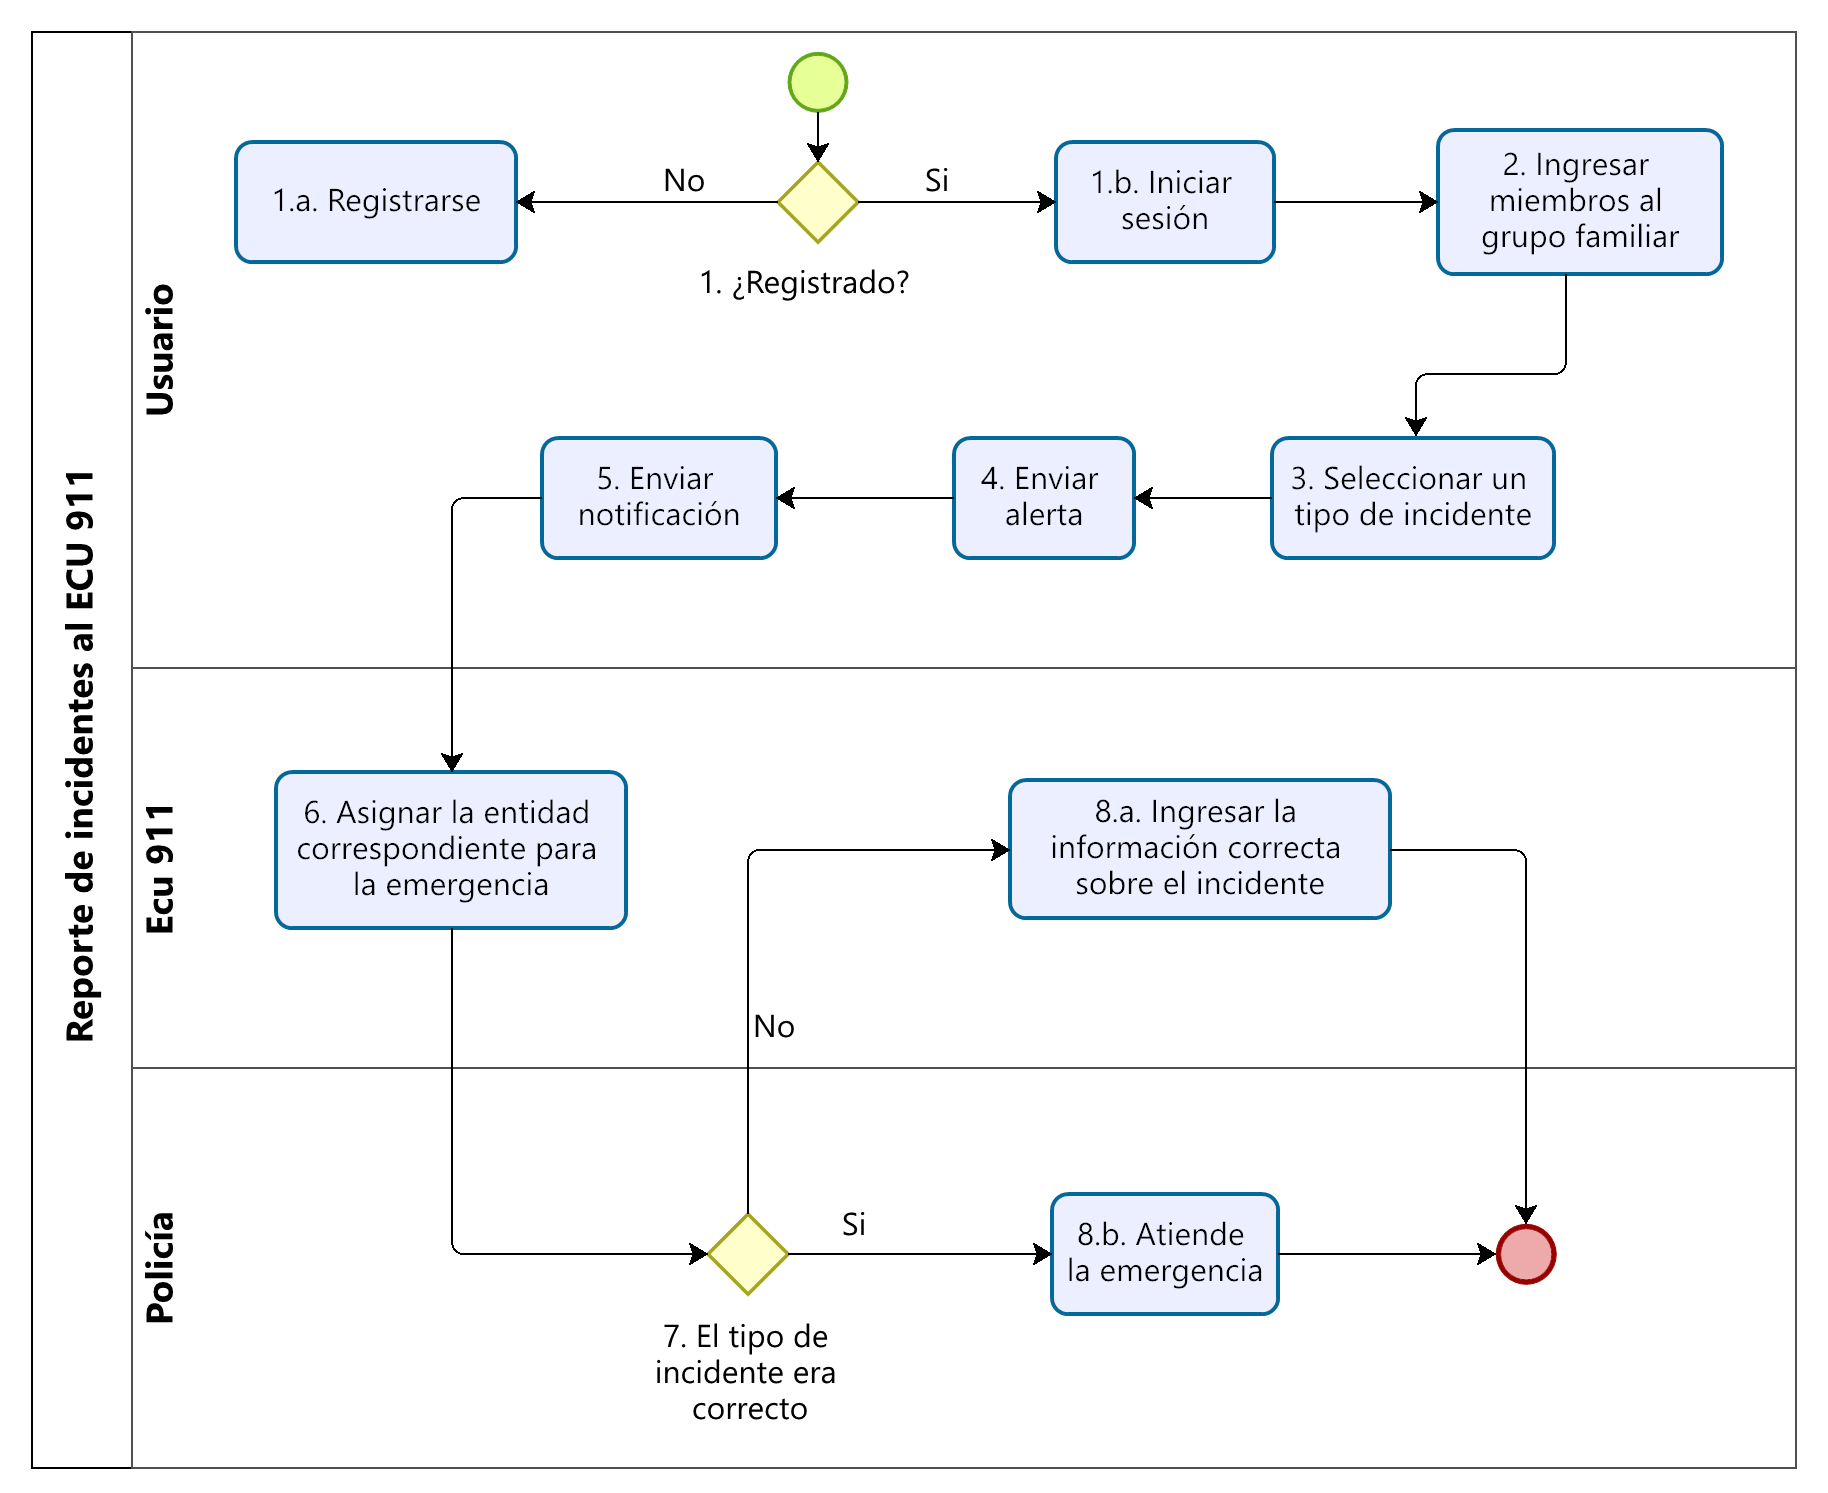
\includegraphics[width=0.8\textwidth]{chapters/III-resultados-y-discusion/resources/images/proceso-propuesto.png}
    \caption{Proceso propuesto de reporte de incidentes al ECU 911.}
    \label{fig:proceso-propuesto}
\end{figure}

\subsubsection{Arquitectura}

El desarrollo del sistema se estructuró en 2 partes fundamentales: la API y La interfaz de usuario, tanto web como móvil.
La interfaz de usuario en el sistema web permite a los administradores gestionar la información de los usuarios y los incidentes
ademas de visualizar la ubicación en tiempo real de los incidentes en un mapa. La interfaz de usuario en el sistema móvil
permite gestionar grupos familiares, enviar alertas de emergencia y visualizar la ubicación en tiempo real de los incidentes de sus
miembros del grupo familiar. El API se encuentra alojada en un servidor web y se encarga de gestionar la conexión entre la base de
datos, los servicios de almacenamiento de información, el servicio de hosting de imágenes, el servicio de web socket y las interfaces
de usuario.

\begin{figure}[H]
    \centering
    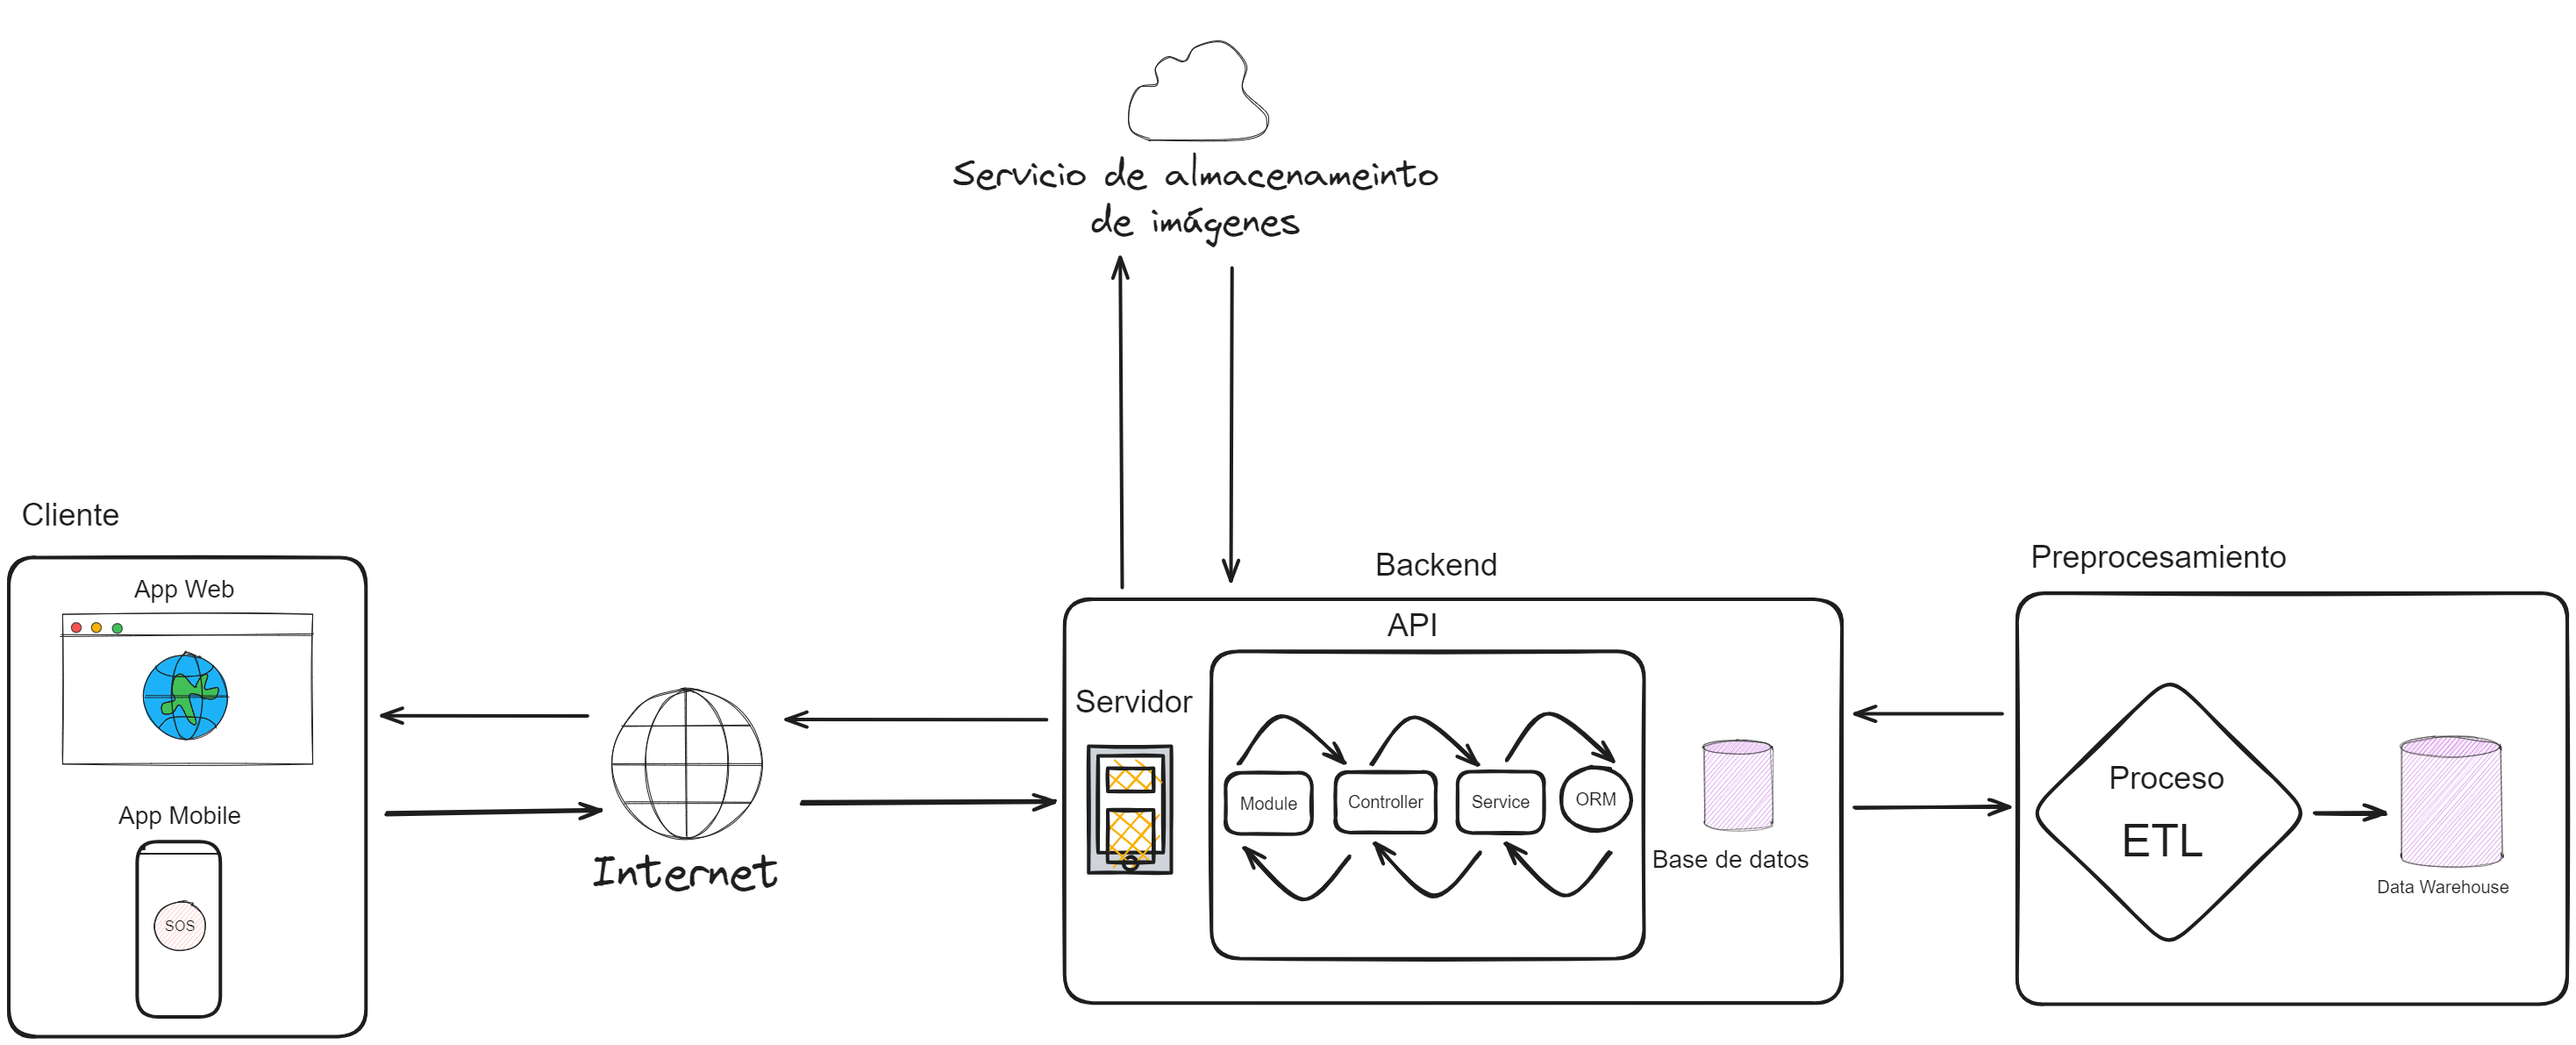
\includegraphics[width=1.1\textwidth]{chapters/III-resultados-y-discusion/resources/images/arquitectura.png}
    \caption{Arquitectura del sistema}
    \label{fig:arquitectura}
\end{figure}


\subsubsection{Prototipado}

En esta etapa de la metodología, se desarrollaron prototipos con el objetivo de identificar y resolver problemas de diseño y funcionalidad.
Esto permite detectar posibles fallos o áreas de mejora antes de la fase de construcción de la aplicación, optimizando así el proceso de
desarrollo y asegurando que el producto final sea más robusto y alineado con los objetivos del proyecto.

El prototipado para el sistema se divide en dos partes: el prototipo de la interfaz de usuario web y el prototipo de la interfaz de usuario móvil.

\subsubsection{Prototipo de la interfaz de usuario web}

En la Figura \ref{fig:prototipo-inicio-sesion-web} se presenta el prototipo de la interfaz de usuario web, donde se muestra la pantalla de inicio de sesión,
el cual se realiza mediante correo y contraseña.

\begin{figure}[H]
    \centering
    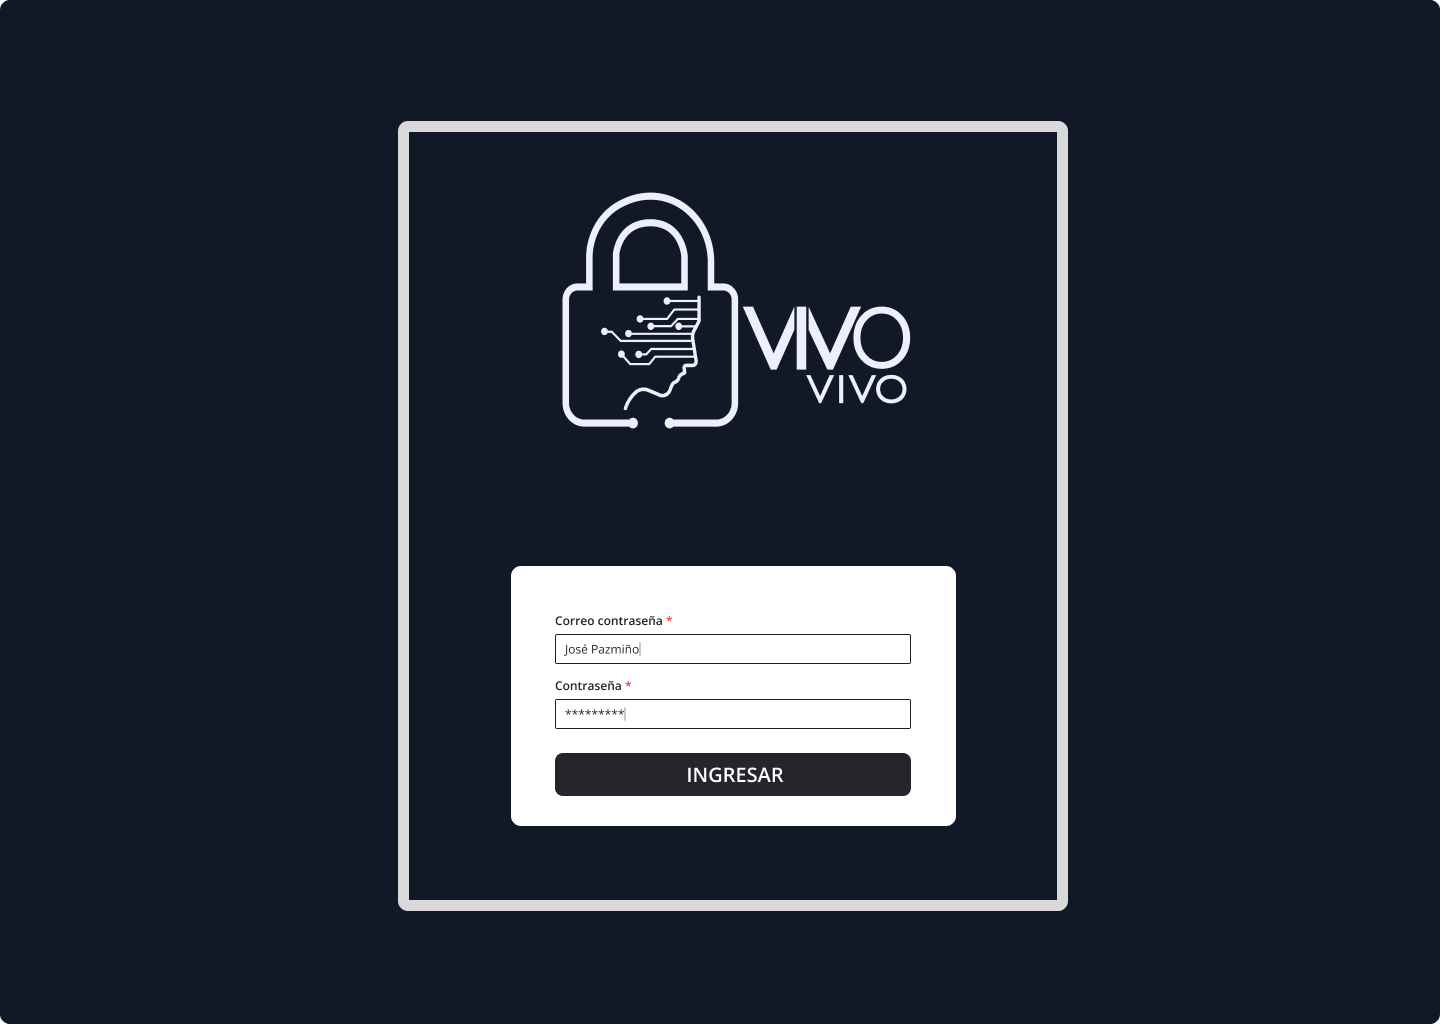
\includegraphics[width=0.6\textwidth]{chapters/III-resultados-y-discusion/resources/images/prototipo-inicio-sesion-web.png}
    \caption{Prototipo de la interfaz de usuario web: Inicio de sesión.}
    \label{fig:prototipo-inicio-sesion-web}
\end{figure}

En la Figura \ref{fig:prototipo-layout-web} se presenta el prototipo de la interfaz de usuario web, donde se muestra el layout de la aplicación web junto
con el menú de navegación y el menú de opciones

\begin{figure}[H]
    \centering
    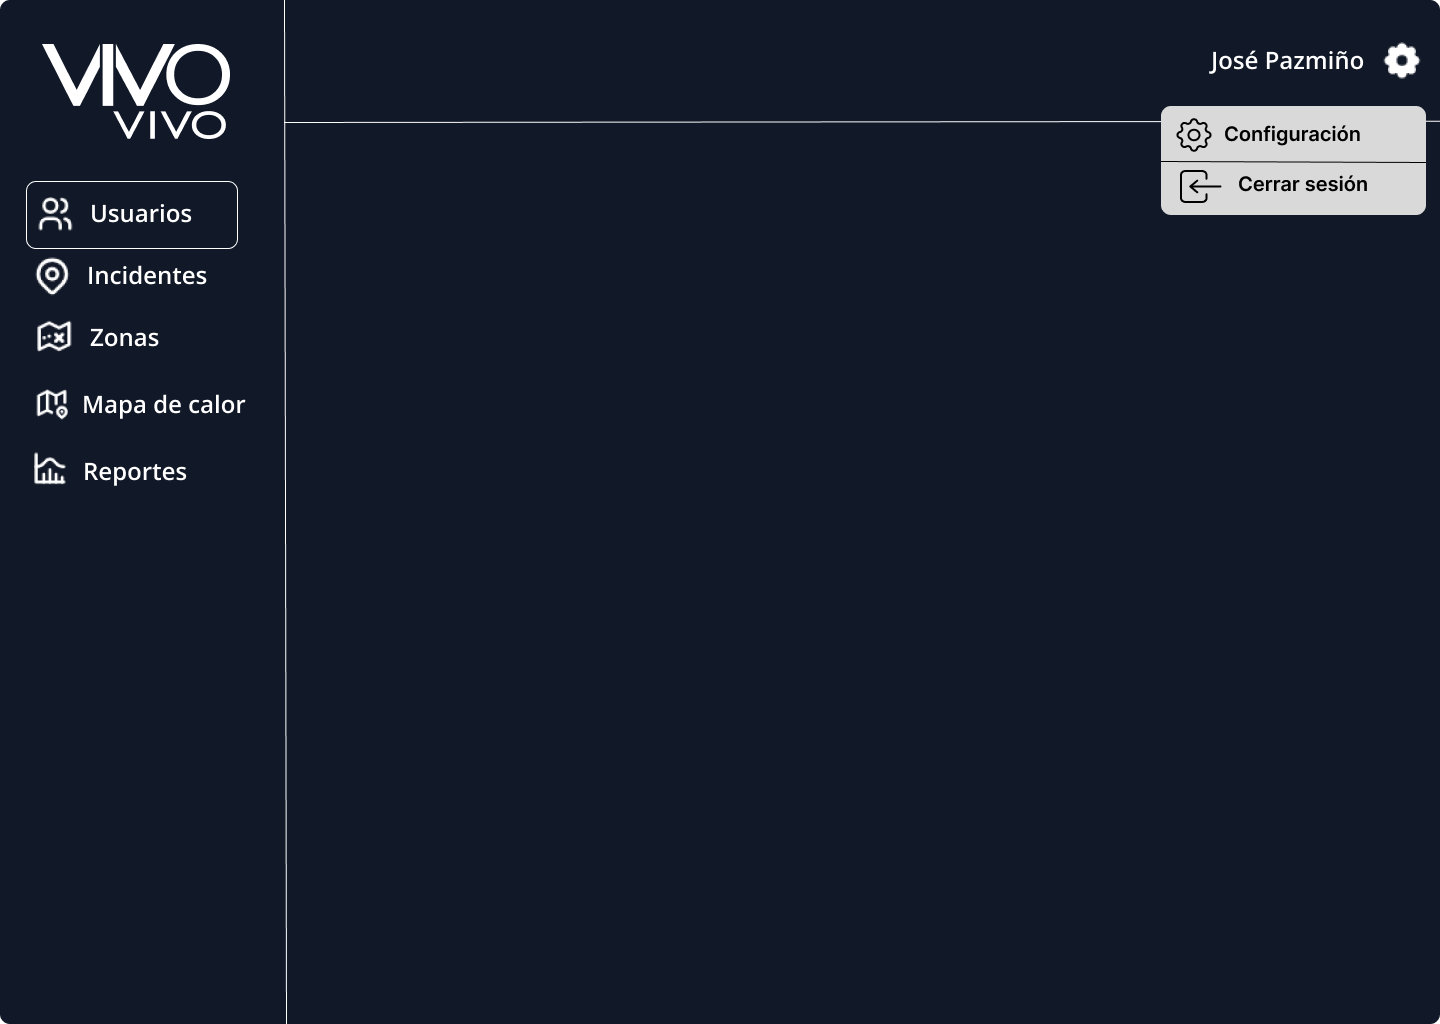
\includegraphics[width=0.6\textwidth]{chapters/III-resultados-y-discusion/resources/images/prototipo-layout-web.png}
    \caption{Prototipo de la interfaz de usuario web: Layout.}
    \label{fig:prototipo-layout-web}
\end{figure}

La gestión de la información en el sistema web se realiza a través de una tabla de entradas, la cual permite al usuario administrador crear, visualizar,
editar y eliminar los registros, así como también aplicar filtros de búsqueda, como se muestra en la Figura \ref{fig:prototipo-tabla-entradas-web}.

\begin{figure}[H]
    \centering
    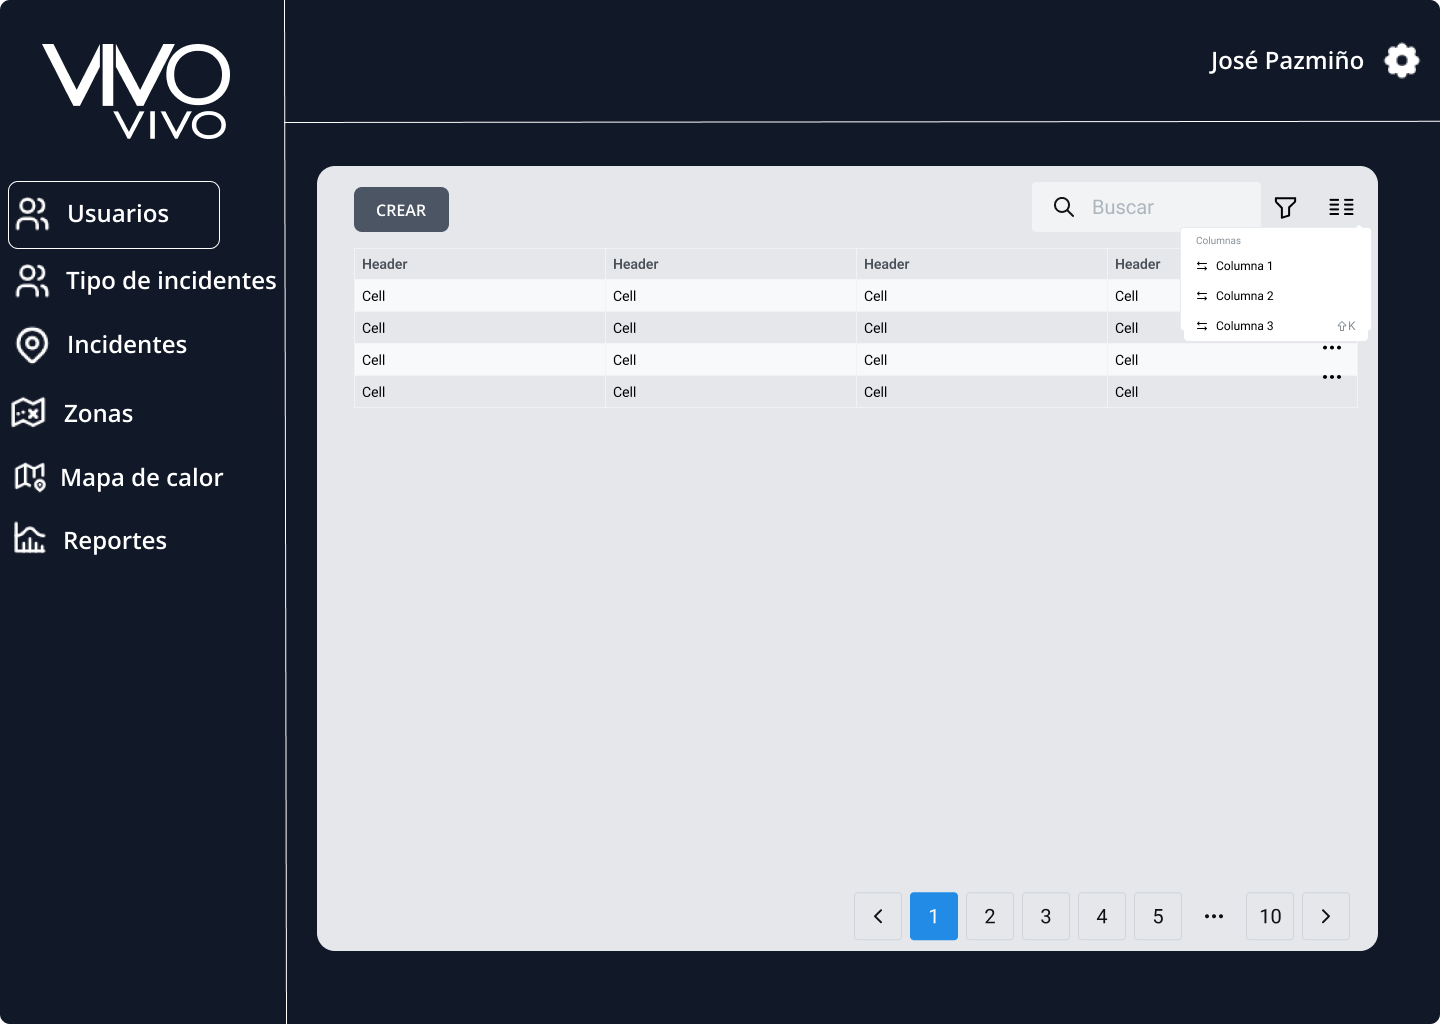
\includegraphics[width=0.6\textwidth]{chapters/III-resultados-y-discusion/resources/images/prototipo-tabla-entradas-web.png}
    \caption{Prototipo de la interfaz de usuario web: Tabla de entradas.}
    \label{fig:prototipo-tabla-entradas-web}
\end{figure}

En la Figura \ref{fig:prototipo-menu-tabla-entradas-web} se muestra el menú de opciones de la tabla de entradas, el cual permite al usuario administrador
realizar acciones como editar y eliminar registros. Al eliminar un registro, se muestra un mensaje de confirmación para ejecutar la acción, como se puede
observar en la Figura \ref{fig:prototipo-mensaje-eliminar-web}

\begin{figure}[H]
    \centering
    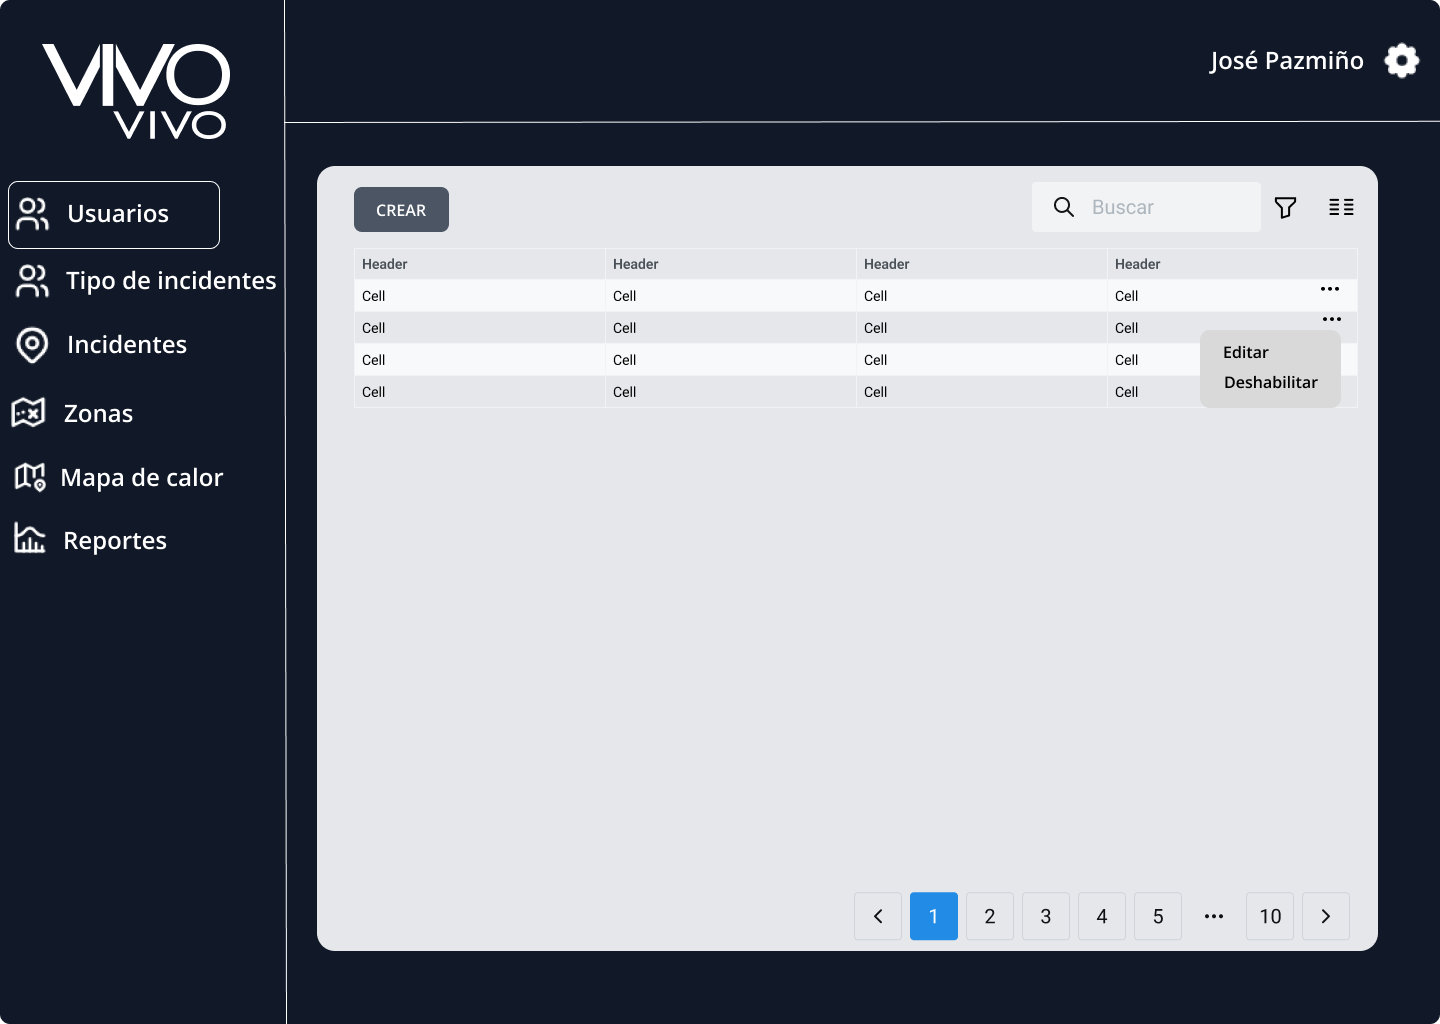
\includegraphics[width=0.6\textwidth]{chapters/III-resultados-y-discusion/resources/images/prototipo-menu-tabla-entradas-web.png}
    \caption{Prototipo de la interfaz de usuario web: Menú de opciones de la tabla de entradas.}
    \label{fig:prototipo-menu-tabla-entradas-web}
\end{figure}

\begin{figure}[H]
    \centering
    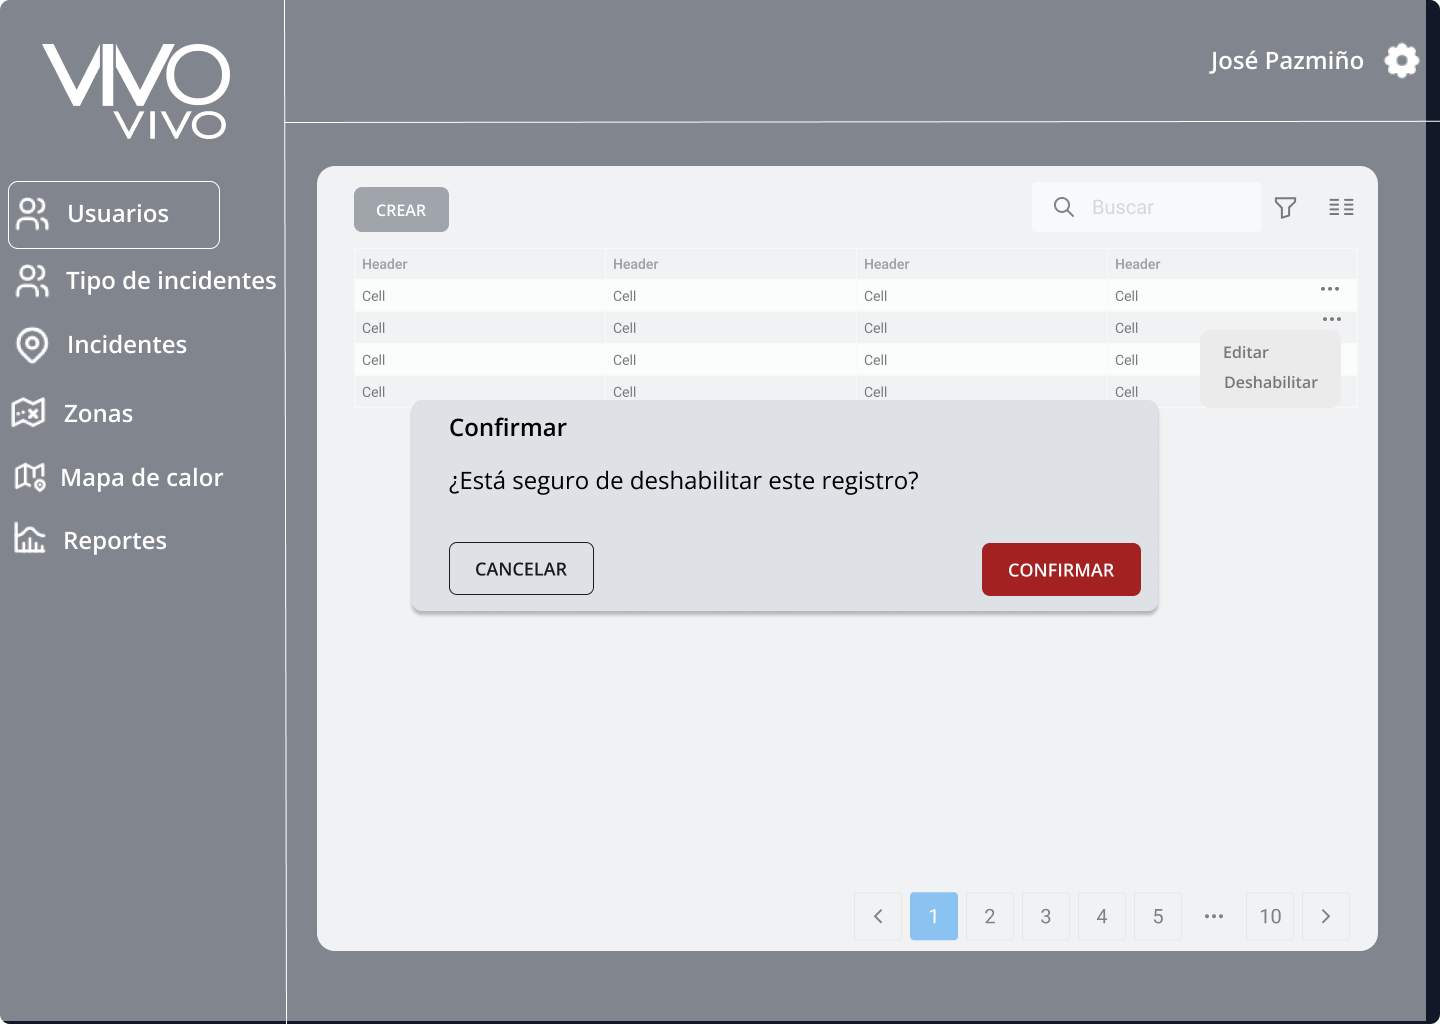
\includegraphics[width=0.6\textwidth]{chapters/III-resultados-y-discusion/resources/images/prototipo-mensaje-eliminar-web.png}
    \caption{Prototipo de la interfaz de usuario web: Mensaje de confirmación para eliminar un registro.}
    \label{fig:prototipo-mensaje-eliminar-web}
\end{figure}

Para la gestión de usuarios en el sistema web, la informaci��n de dichos usuarios se visualizará en una tabla, como se puede observar en la Figura
\ref{fig:prototipo-tabla-usuarios-web}. Se propone un formulario de registro en el cual el usuario administrador puede ingresar la información
necesaria para crear un nuevo usuario, así como actualizar la información de un usuario existente y eliminar un usuario, como se muestra en la Figura
\ref{fig:prototipo-formulario-usuario-web}.

\begin{figure}[H]
    \centering
    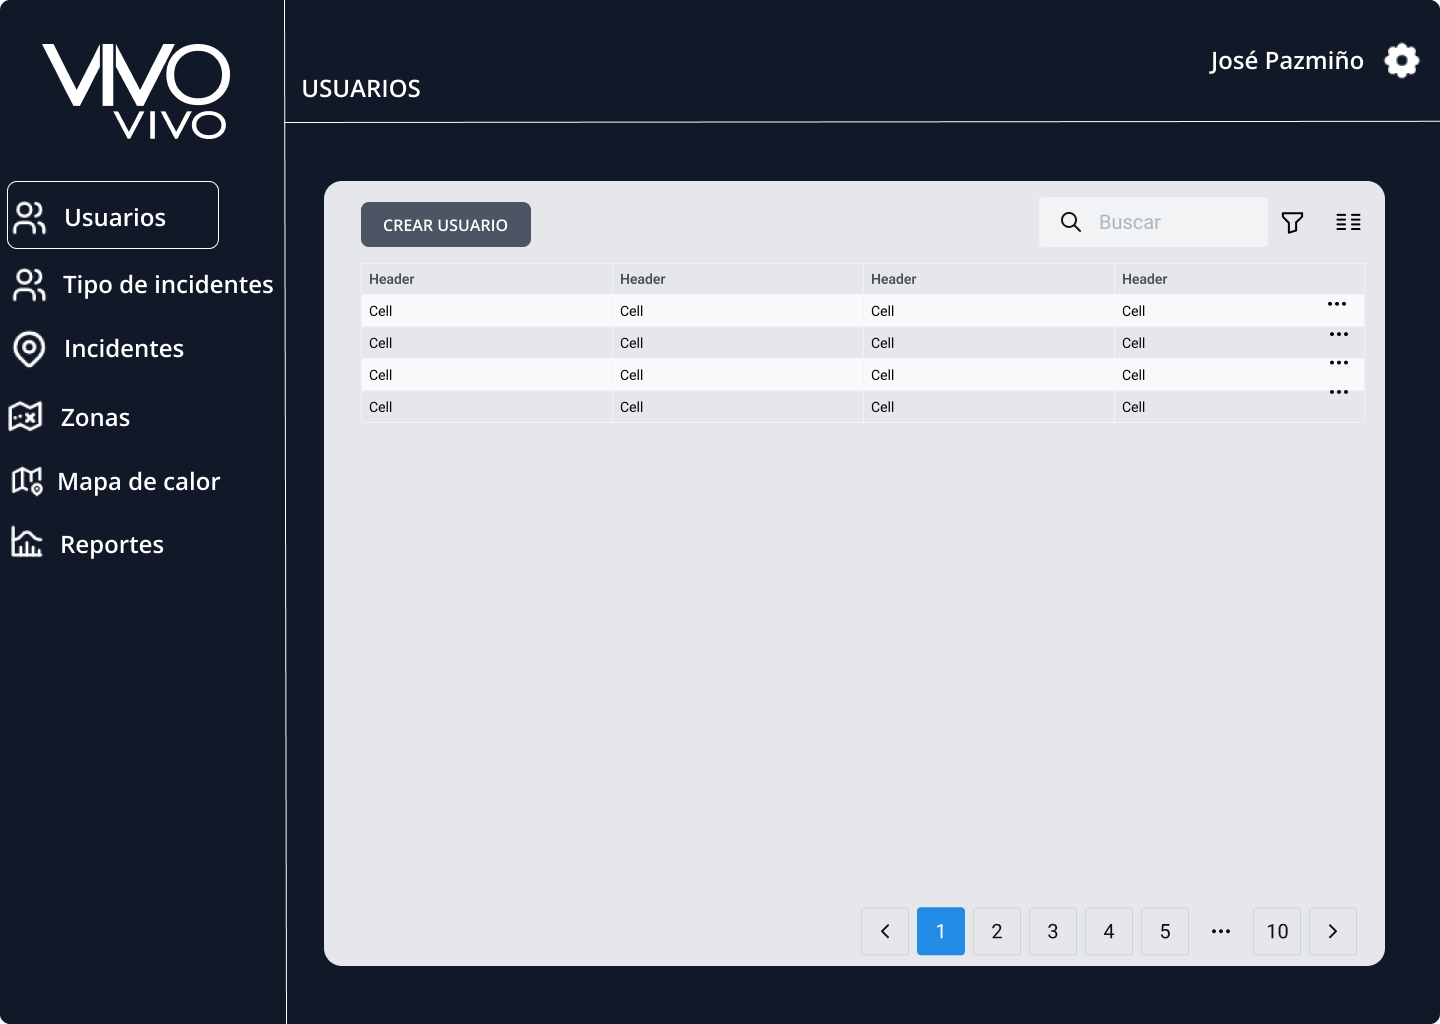
\includegraphics[width=0.6\textwidth]{chapters/III-resultados-y-discusion/resources/images/prototipo-tabla-usuarios-web.png}
    \caption{Prototipo de la interfaz de usuario web: Tabla de usuarios.}
    \label{fig:prototipo-tabla-usuarios-web}
\end{figure}

\begin{figure}[H]
    \centering
    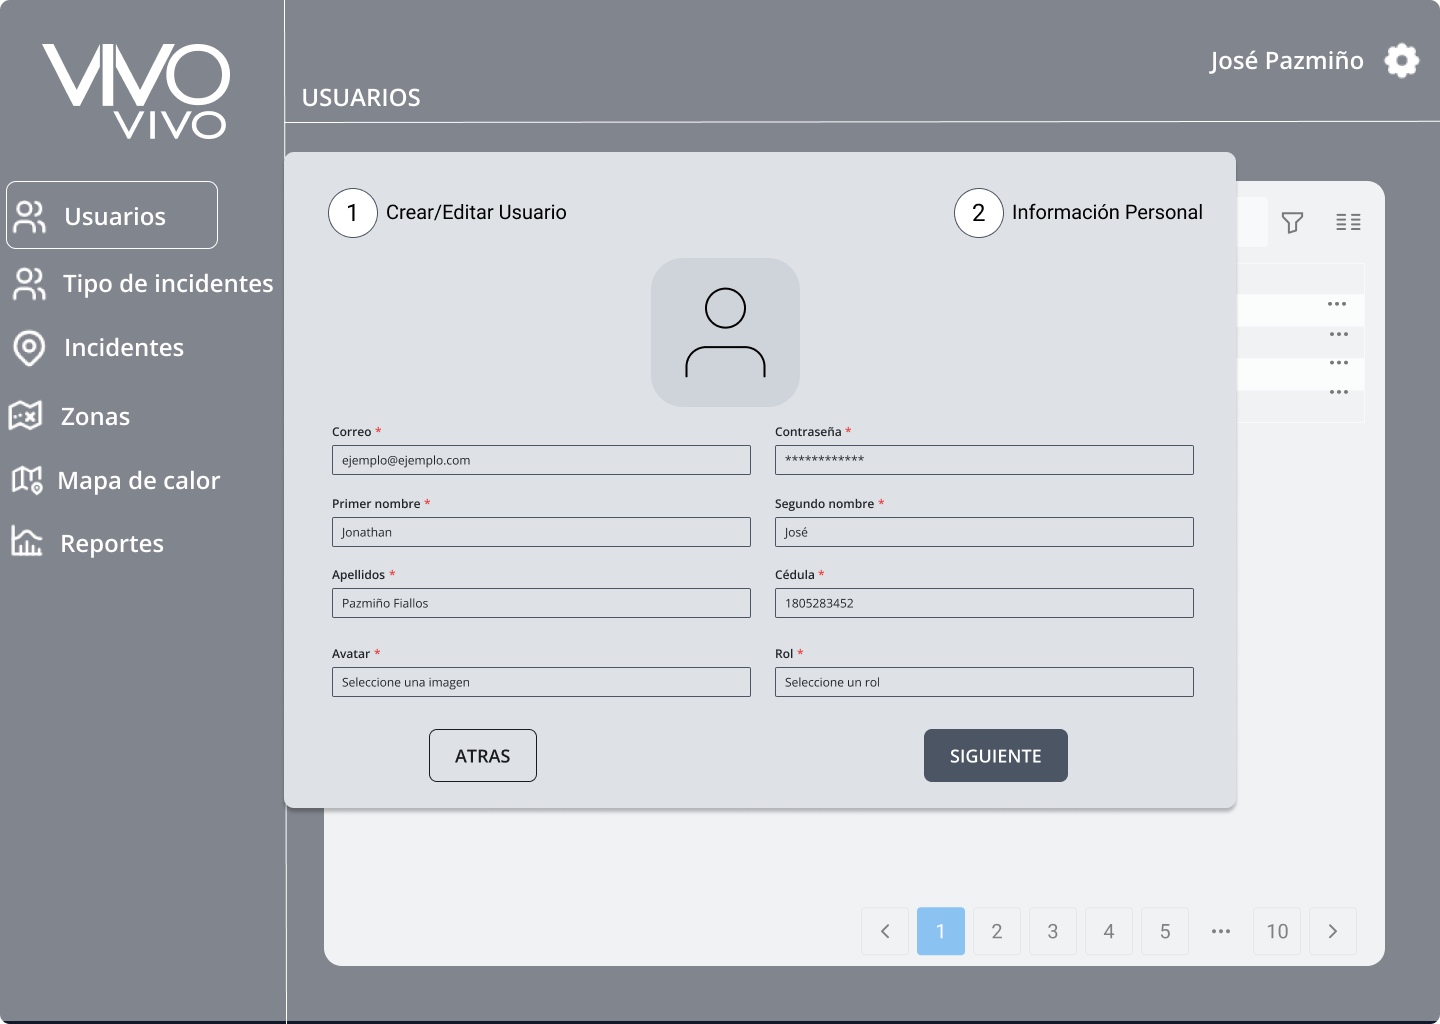
\includegraphics[width=0.6\textwidth]{chapters/III-resultados-y-discusion/resources/images/prototipo-formulario-usuario-web.png}
    \caption{Prototipo de la interfaz de usuario web: Formulario de usuario.}
    \label{fig:prototipo-formulario-usuario-web}
\end{figure}

Para la visualización de la información de los tipos de incidentes en el sistema web, se desarrolló una tabla de entradas, como se muestra en la Figura
\ref{fig:prototipo-tabla-tipos-incidentes-web}. Se propone un formulario de registro en el cual el usuario administrador puede ingresar la información
necesaria para crear un nuevo tipo de incidente, así como actualizar la información de un tipo de incidente existente y eliminar un tipo de incidente,
como se muestra en la Figura \ref{fig:prototipo-formulario-tipo-incidente-web}.

\begin{figure}[H]
    \centering
    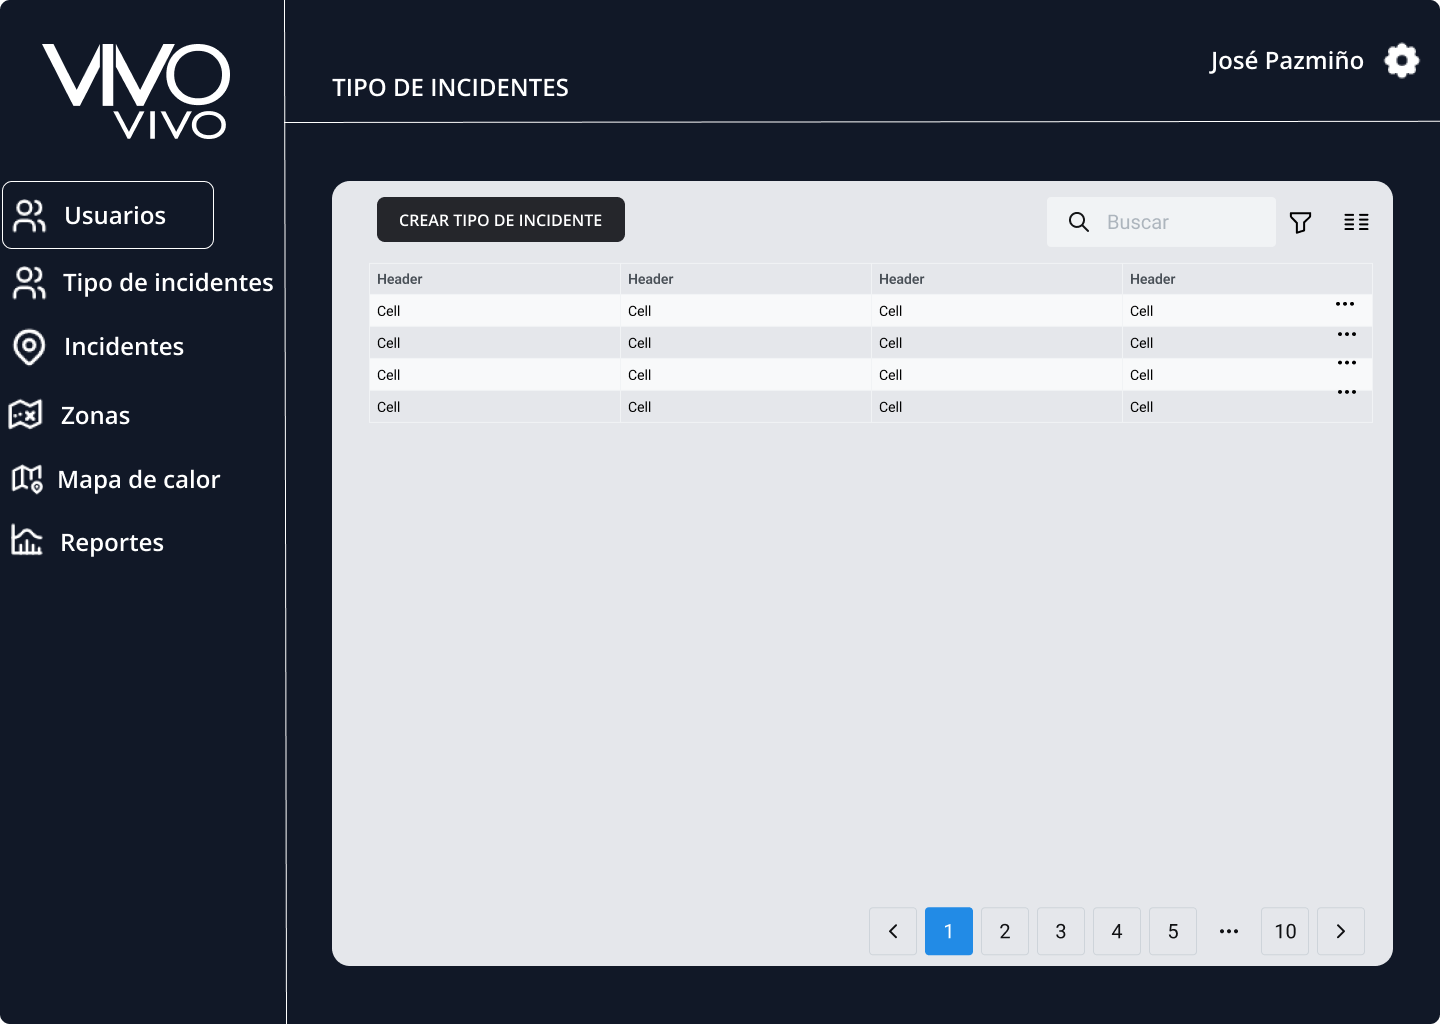
\includegraphics[width=0.6\textwidth]{chapters/III-resultados-y-discusion/resources/images/prototipo-tabla-tipos-incidentes-web.png}
    \caption{Prototipo de la interfaz de usuario web: Tabla de tipos de incidentes.}
    \label{fig:prototipo-tabla-tipos-incidentes-web}
\end{figure}

\begin{figure}[H]
    \centering
    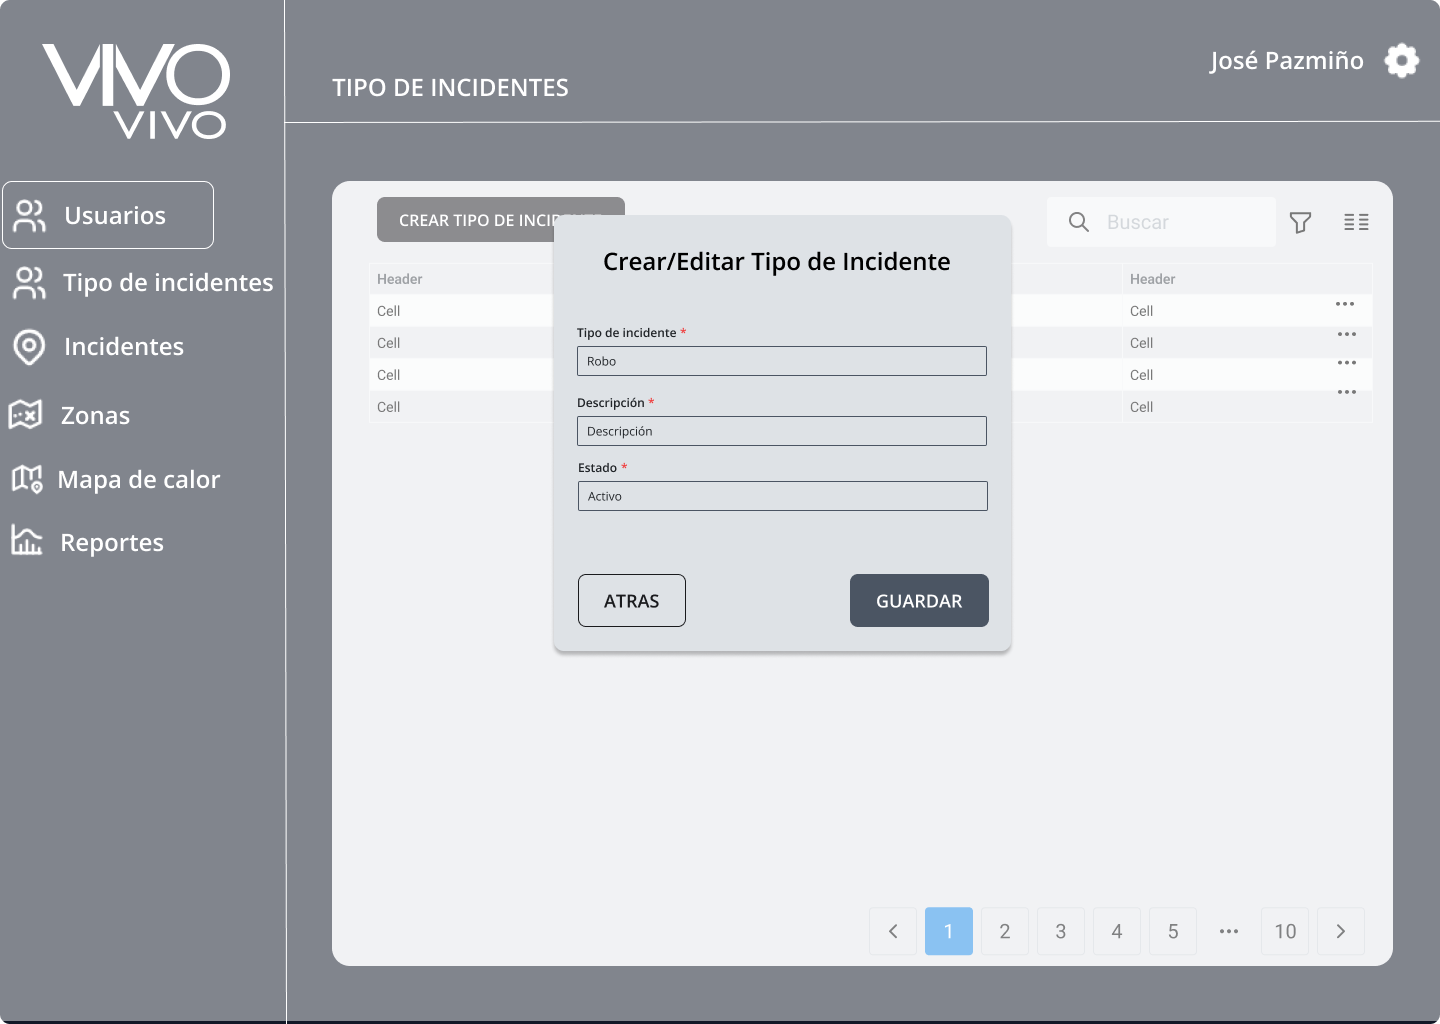
\includegraphics[width=0.6\textwidth]{chapters/III-resultados-y-discusion/resources/images/prototipo-formulario-tipo-incidente-web.png}
    \caption{Prototipo de la interfaz de usuario web: Formulario de tipo de incidente.}
    \label{fig:prototipo-formulario-tipo-incidente-web}
\end{figure}

En la Figura \ref{fig:prototipo-mapa-zonas-de-vigilancia-web} se muestra la pantalla de zonas de vigilancia, la cual permite al usuario administrador
visualizar las zonas de vigilancia mediante polígonos en un mapa interactivo.

\begin{figure}[H]
    \centering
    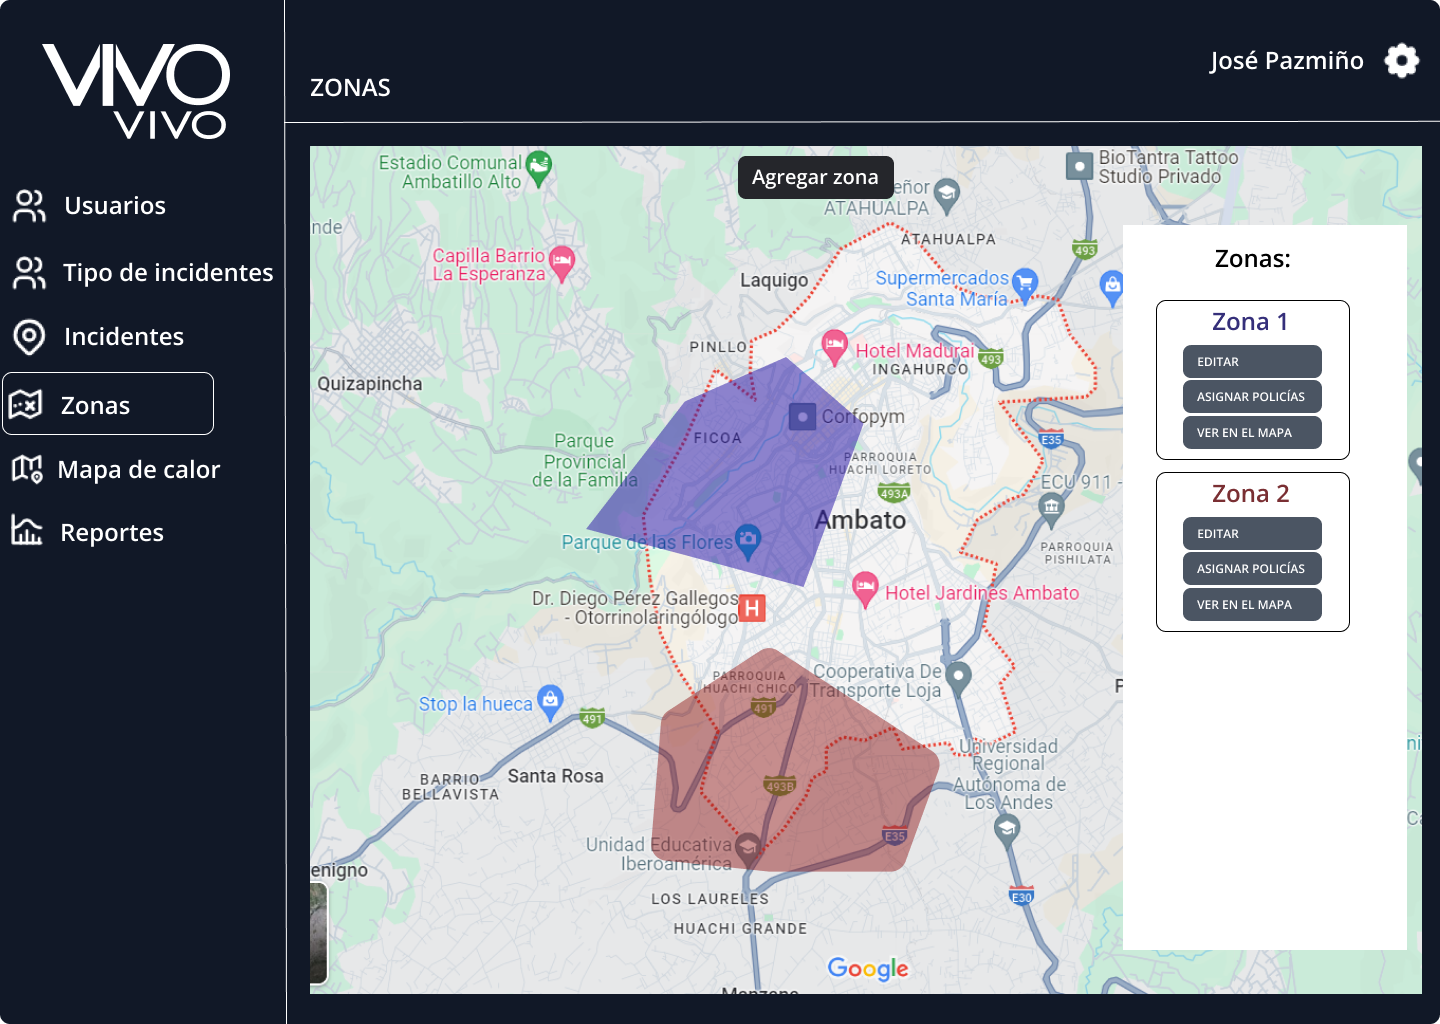
\includegraphics[width=0.6\textwidth]{chapters/III-resultados-y-discusion/resources/images/prototipo-mapa-zonas-de-vigilancia-web.png}
    \caption{Prototipo de la interfaz de usuario web: Mapa de zonas de vigilancia.}
    \label{fig:prototipo-mapa-zonas-de-vigilancia-web}
\end{figure}

Para la creación de zonas de vigilancia, se propone un formulario integrado con el mapa interactivo, el cual permite al usuario administrador
dibujar un polígono en el mapa para definir una zona de vigilancia, como se muestra en la Figura \ref{fig:prototipo-formulario-zona-vigilancia-web}.

\begin{figure}[H]
    \centering
    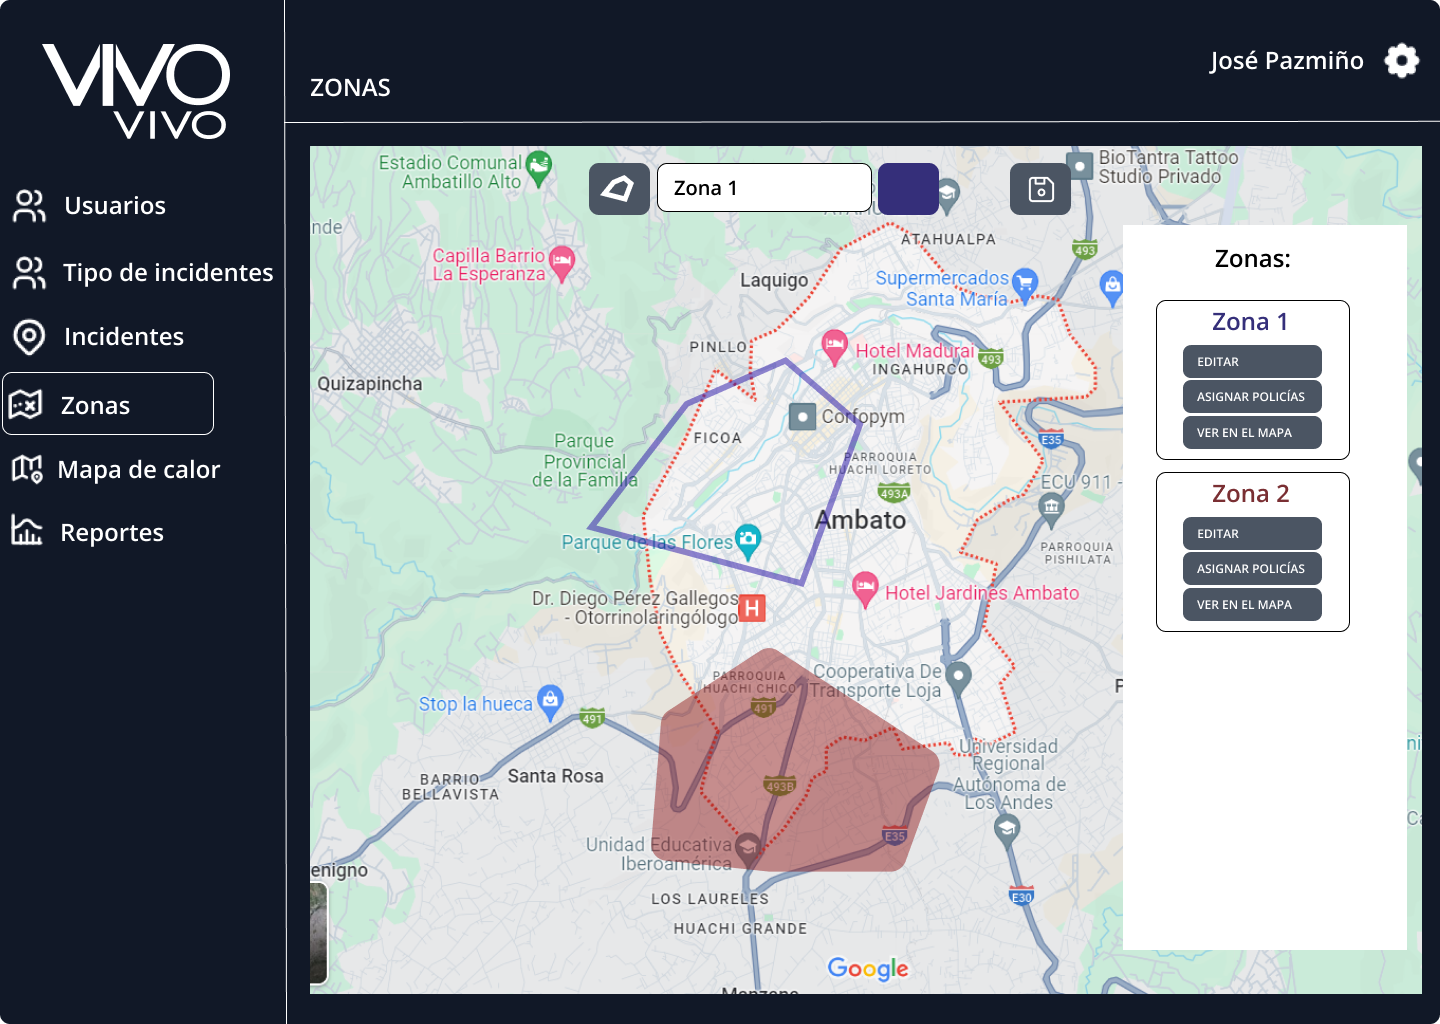
\includegraphics[width=0.6\textwidth]{chapters/III-resultados-y-discusion/resources/images/prototipo-formulario-zona-vigilancia-web.png}
    \caption{Prototipo de la interfaz de usuario web: Formulario de zona de vigilancia.}
    \label{fig:prototipo-formulario-zona-vigilancia-web}
\end{figure}

La pantalla de mapa de incidentes permite al usuario administrador visualizar los incidentes reportados en un mapa interactivo junto con la
ubicación en tiempo real de la víctima, como se muestra en la Figura \ref{fig:prototipo-mapa-incidentes-web}.

\begin{figure}[H]
    \centering
    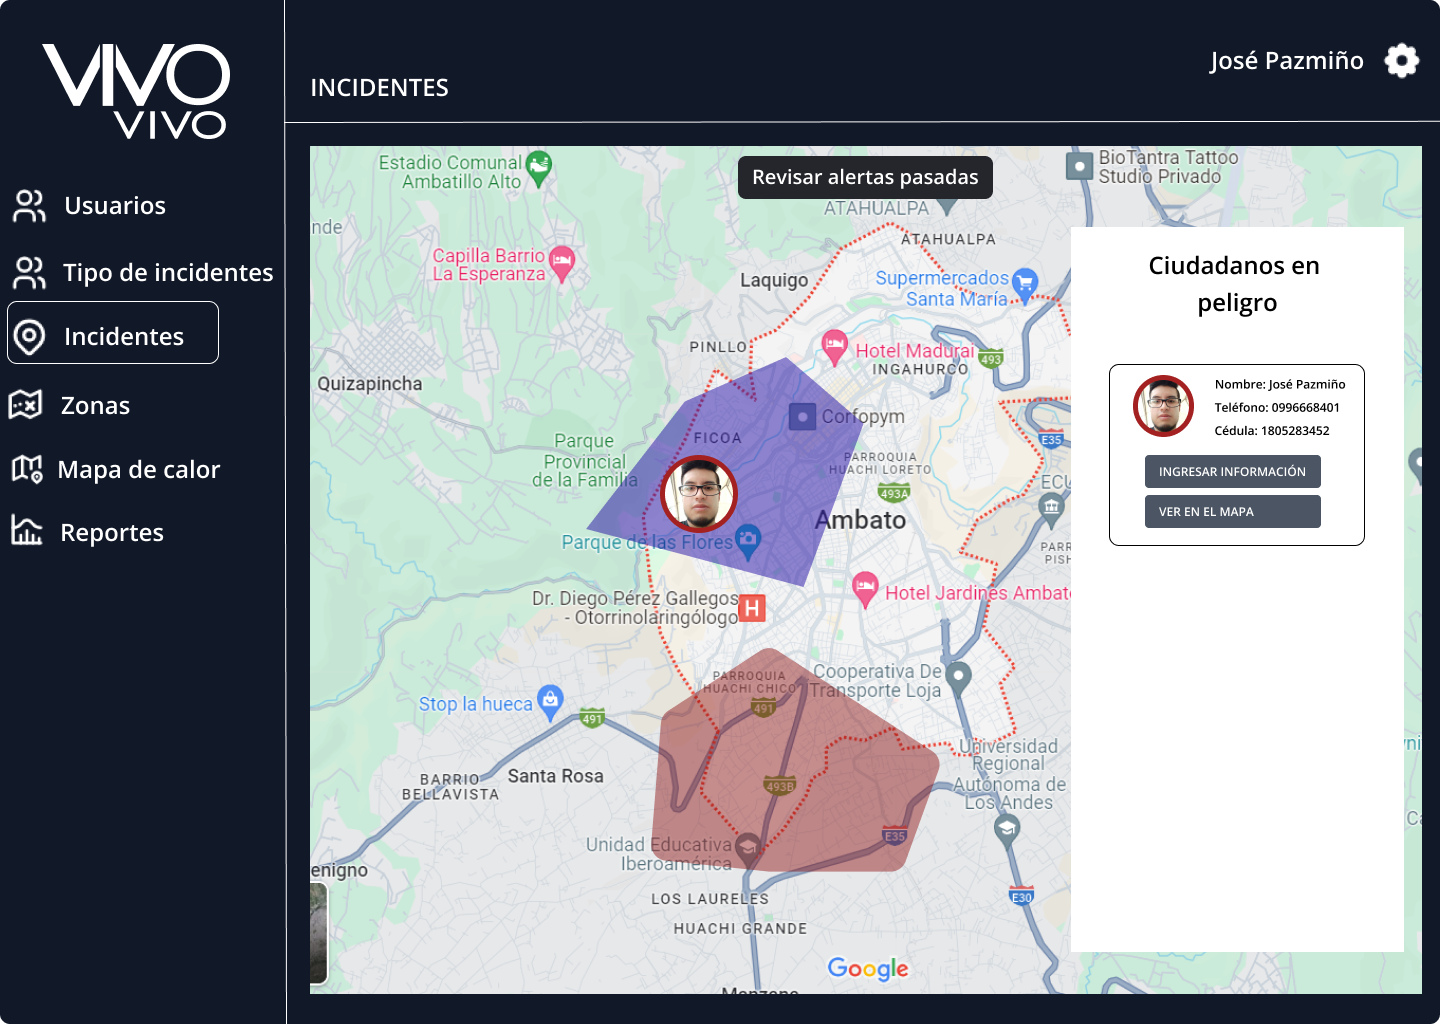
\includegraphics[width=0.6\textwidth]{chapters/III-resultados-y-discusion/resources/images/prototipo-mapa-incidentes-web.png}
    \caption{Prototipo de la interfaz de usuario web: Mapa de incidentes.}
    \label{fig:prototipo-mapa-incidentes-web}
\end{figure}

En la Figura \ref{fig:prototipo-mapa-de-calor-web} se muestra la pantalla de mapa de calor, la cual permite al usuario administrador visualizar
la densidad de incidentes reportados en un mapa interactivo mediante un gradiente de colores, así como filtrar los incidentes por tipo y fecha.

\begin{figure}[H]
    \centering
    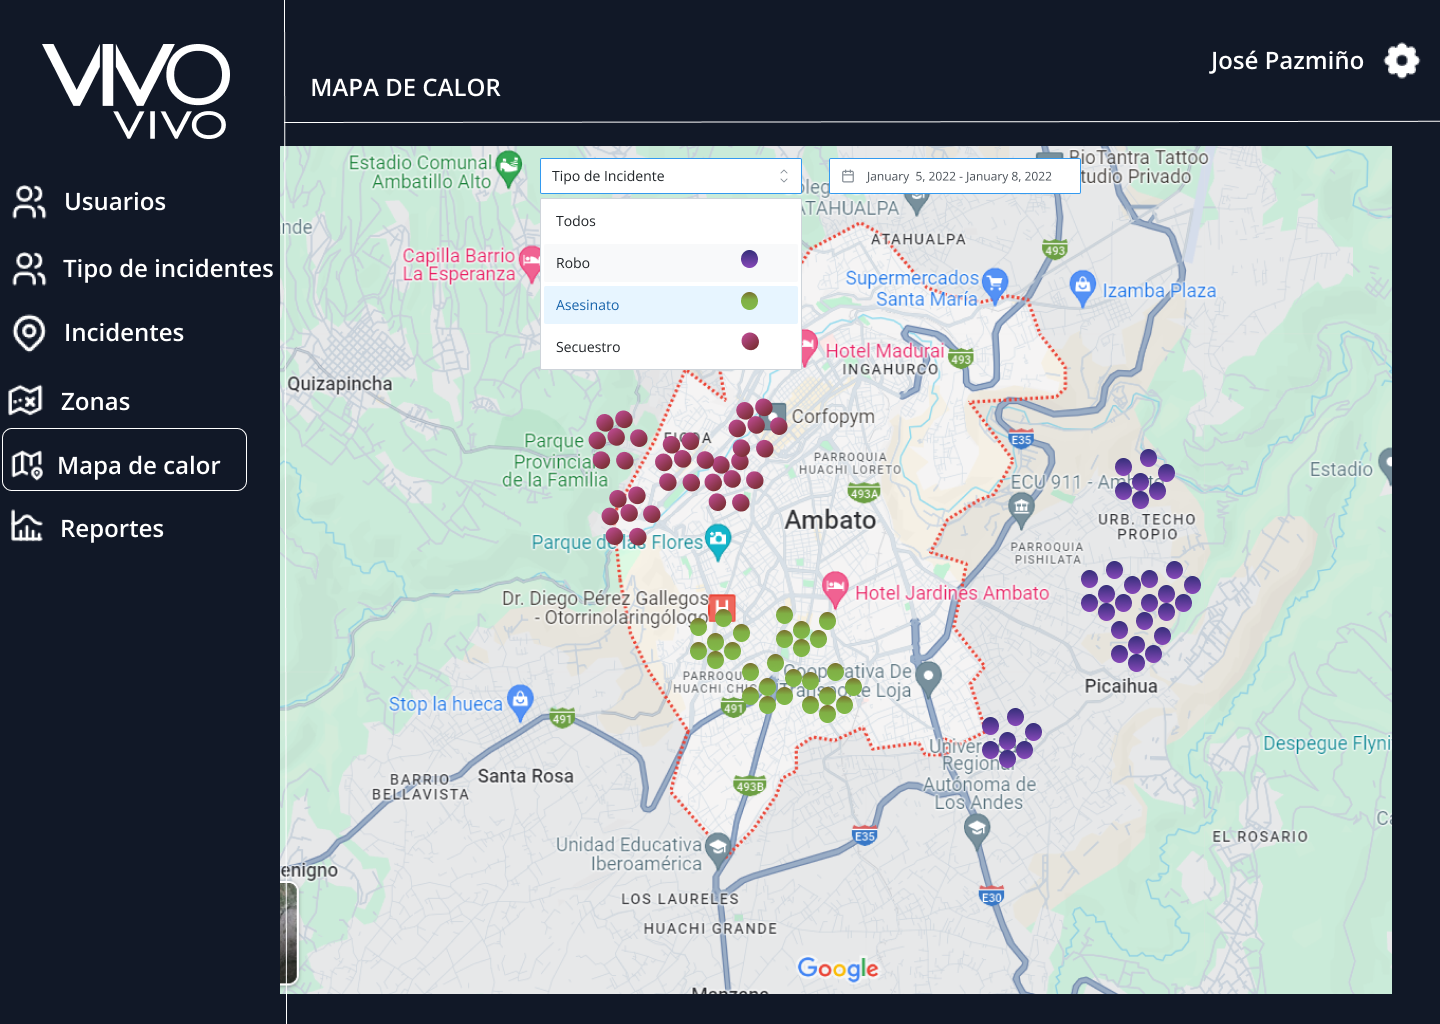
\includegraphics[width=0.6\textwidth]{chapters/III-resultados-y-discusion/resources/images/prototipo-mapa-de-calor-web.png}
    \caption{Prototipo de la interfaz de usuario web: Mapa de calor.}
    \label{fig:prototipo-mapa-de-calor-web}
\end{figure}

En la pantalla de reportería, el usuario administrador puede visualizar gráficos estadísticos de los incidentes reportados, tal como se muestra
en la Figura \ref{fig:prototipo-reporteria-web}.

\begin{figure}[H]
    \centering
    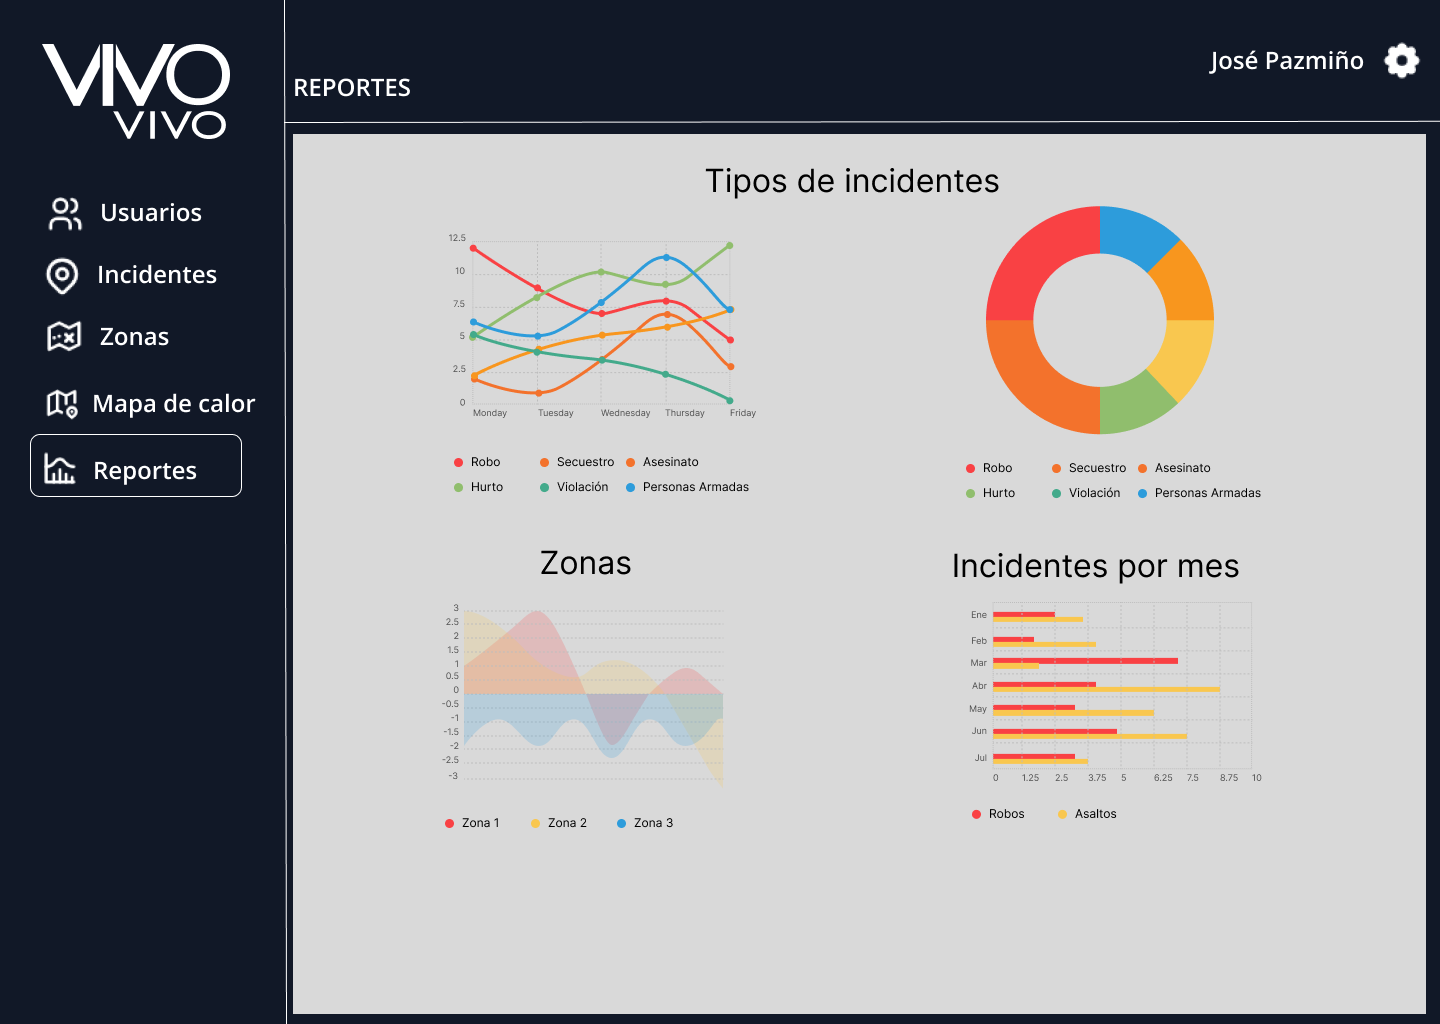
\includegraphics[width=0.6\textwidth]{chapters/III-resultados-y-discusion/resources/images/prototipo-reporteria-web.png}
    \caption{Prototipo de la interfaz de usuario web: Reportería.}
    \label{fig:prototipo-reporteria-web}
\end{figure}

\subsubsection{Prototipo de la interfaz de usuario móvil}
% TODO: REVISAR ORTOGRAFÍA
En la Figura \ref{fig:prototipo-inicio-sesion-mobile} se muestra la pantalla de inicio de sesión en la aplicación móvil, la cual se realiza mediante
el correo y contraseña del usuario.

\begin{figure}[H]
    \centering
    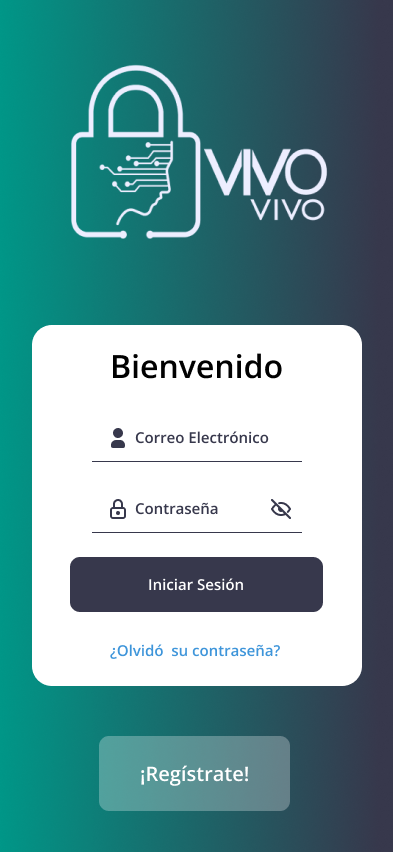
\includegraphics[width=0.3\textwidth]{chapters/III-resultados-y-discusion/resources/images/prototipo-inicio-sesion-mobile.png}
    \caption{Prototipo de la interfaz de usuario móvil: Inicio de sesión.}
    \label{fig:prototipo-inicio-sesion-mobile}
\end{figure}

Para el registro de usuarios se propone un formulario en el cual se ingresan una fotografía, nombres, apellidos, etnia, género, estado civil,
discapacidad en caso de presentarla y dirección, tal como se muestra en la Figura \ref{fig:prototipo-registro-mobile}.

\begin{figure}[H]
    \centering
    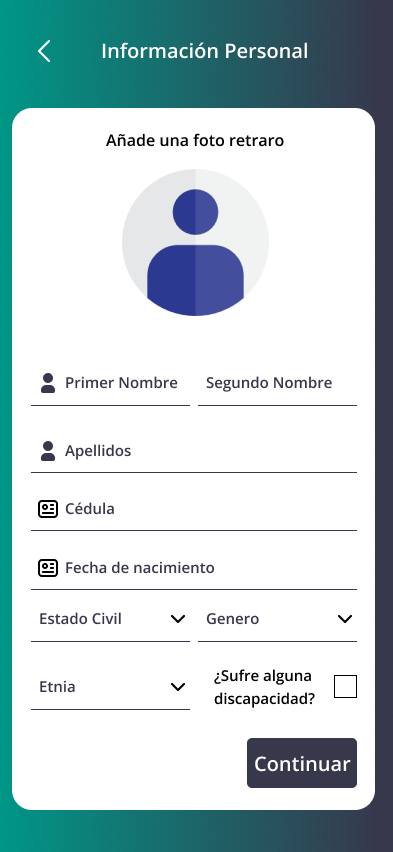
\includegraphics[width=0.3\textwidth]{chapters/III-resultados-y-discusion/resources/images/prototipo-registro-mobile.png}
    \caption{Prototipo de la interfaz de usuario móvil: Registro.}
    \label{fig:prototipo-registro-mobile}
\end{figure}

En la Figura \ref{fig:prototipo-recuperar-contrasena-mobile} se muestra la pantalla de recuperación de contraseña en la aplicación móvil, la cual se realiza
mediante el correo electrónico del usuario.

\begin{figure}[H]
    \centering
    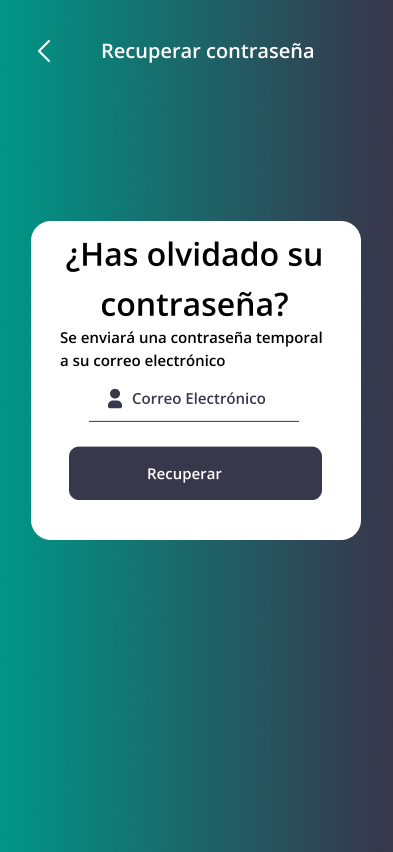
\includegraphics[width=0.3\textwidth]{chapters/III-resultados-y-discusion/resources/images/prototipo-recuperar-contrasena-mobile.png}
    \caption{Prototipo de la interfaz de usuario móvil: Recuperación de contraseña.}
    \label{fig:prototipo-recuperar-contrasena-mobile}
\end{figure}

Para la pantalla de inicio, se propone un botón de pánico que permite al usuario enviar una alerta de emergencia seleccionando el tipo de incidente y
presionando el botón durante 3 segundos para enviar la alerta. En la esquina superior derecha se encuentra el menú de opciones de la aplicación y en la
esquina superior izquierda se encuentra el botón de notificaciones de alertas de emergencia, como se muestra en la Figura \ref{fig:prototipo-inicio-mobile}.

\begin{figure}[H]
    \centering
    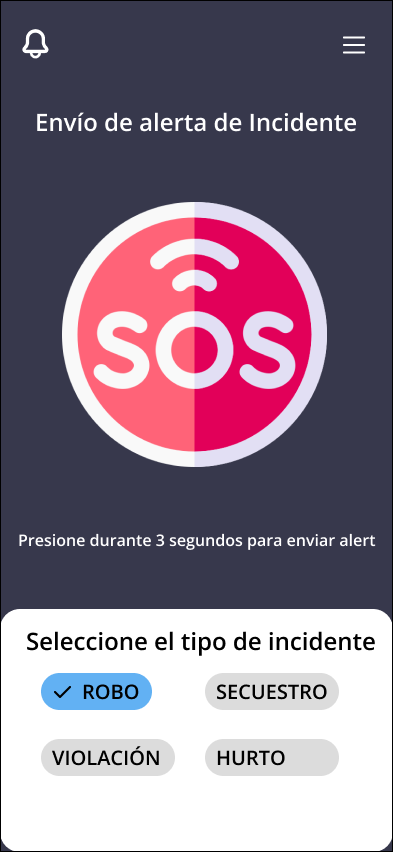
\includegraphics[width=0.3\textwidth]{chapters/III-resultados-y-discusion/resources/images/prototipo-inicio-mobile.png}
    \caption{Prototipo de la interfaz de usuario móvil: Inicio.}
    \label{fig:prototipo-inicio-mobile}
\end{figure}

En la Figura  \ref{fig:prototipo-alertas-mobile} se muestra la pantalla de alertas de emergencia, el usuario puede visualizar las alertas de emergencia
enviadas por los miembros del grupo familiar mediante una lista de alertas con la información de la persona y un botón para visualizar la ubicación
en tiempo real del incidente en un mapa interactivo como se puede observar en la Figura \ref{fig:prototipo-ubicacion-alerta-mobile}.

\begin{figure}[H]
    \centering
    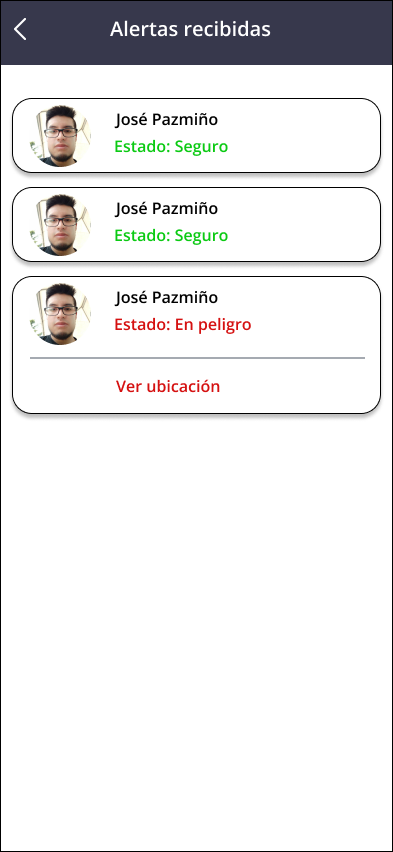
\includegraphics[width=0.3\textwidth]{chapters/III-resultados-y-discusion/resources/images/prototipo-alertas-mobile.png}
    \caption{Prototipo de la interfaz de usuario móvil: Alertas de emergencia.}
    \label{fig:prototipo-alertas-mobile}
\end{figure}

\begin{figure}[H]
    \centering
    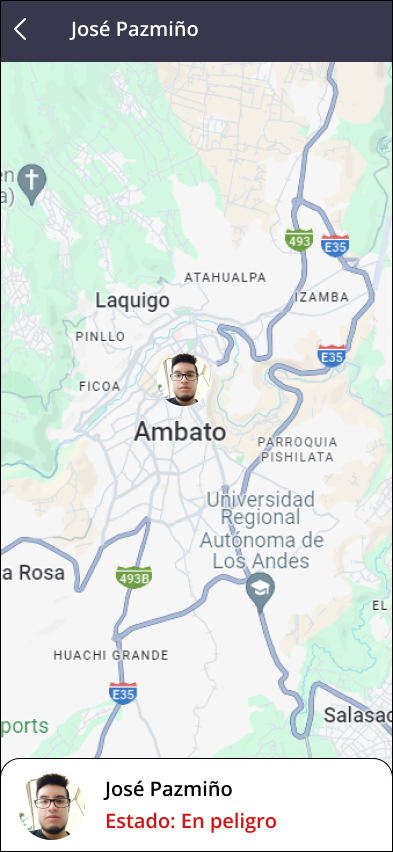
\includegraphics[width=0.3\textwidth]{chapters/III-resultados-y-discusion/resources/images/prototipo-ubicacion-alerta-mobile.png}
    \caption{Prototipo de la interfaz de usuario móvil: Ubicación de alerta.}
    \label{fig:prototipo-ubicacion-alerta-mobile}
\end{figure}

El menú de opciones de la aplicación móvil permite al usuario gestionar su grupo familiar, cambiar su contraseña y cerrar sesión, como se muestra
en la Figura \ref{fig:prototipo-menu-mobile}.

\begin{figure}[H]
    \centering
    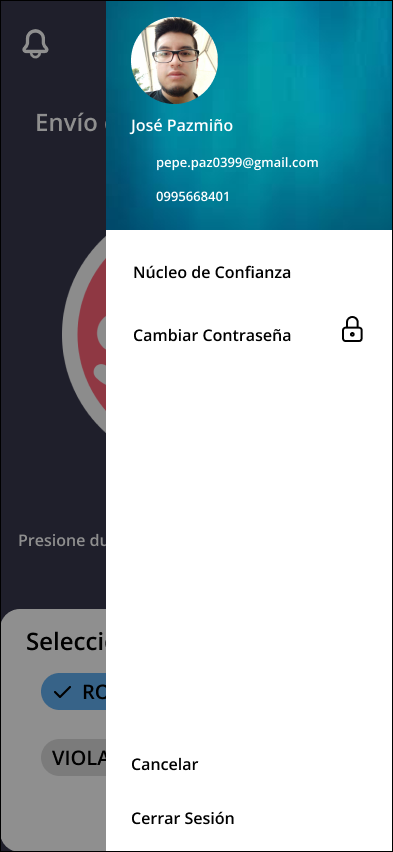
\includegraphics[width=0.3\textwidth]{chapters/III-resultados-y-discusion/resources/images/prototipo-menu-mobile.png}
    \caption{Prototipo de la interfaz de usuario móvil: Menú.}
    \label{fig:prototipo-menu-mobile}
\end{figure}

Para la gestión de grupos familiares, se propone una pantalla en la cual el usuario puede visualizar los miembros de su grupo familiar y agregar
nuevos miembros, como se muestra en la Figura \ref{fig:prototipo-grupo-familiar-mobile}. Al agregar un nuevo miembro, se muestra un formulario
en el cual se puede buscar un usuario por su cédula de identidad y agregarlo al grupo familiar, como se muestra en la Figura \ref{fig:prototipo-agregar-miembro-mobile}.

\begin{figure}[H]
    \centering
    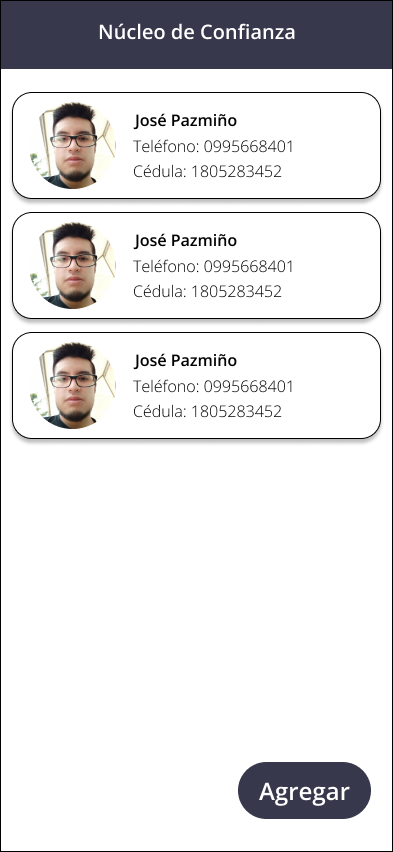
\includegraphics[width=0.3\textwidth]{chapters/III-resultados-y-discusion/resources/images/prototipo-grupo-familiar-mobile.png}
    \caption{Prototipo de la interfaz de usuario móvil: Grupo familiar.}
    \label{fig:prototipo-grupo-familiar-mobile}
\end{figure}

\begin{figure}[H]
    \centering
    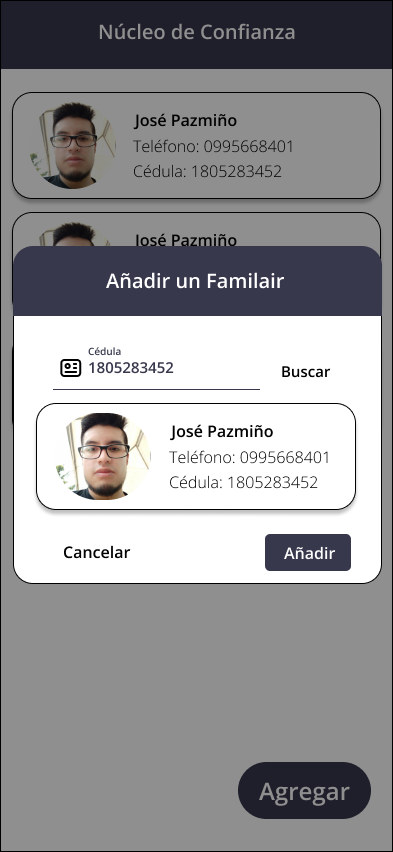
\includegraphics[width=0.3\textwidth]{chapters/III-resultados-y-discusion/resources/images/prototipo-agregar-miembro-mobile.png}
    \caption{Prototipo de la interfaz de usuario móvil: Agregar miembro.}
    \label{fig:prototipo-agregar-miembro-mobile}
\end{figure}

En la Figura \ref{fig:prototipo-cambiar-contrasena-mobile} se muestra la pantalla para cambiar la contraseña en la aplicación móvil. El usuario
debe ingresar su contraseña actual, la nueva contraseña y confirmar la nueva contraseña para realizar el cambio.

\begin{figure}[H]
    \centering
    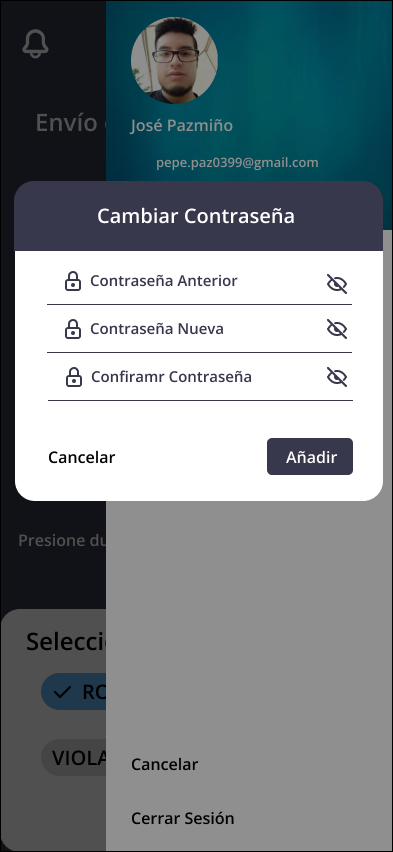
\includegraphics[width=0.3\textwidth]{chapters/III-resultados-y-discusion/resources/images/prototipo-cambiar-contrasena-mobile.png}
    \caption{Prototipo de la interfaz de usuario móvil: Cambiar contraseña.}
    \label{fig:prototipo-cambiar-contrasena-mobile}
\end{figure}

% \subsection{Construcción}

En esta sección se describe la construcción de la propuesta del sistema, la cual se divide en dos partes fundamentales: la API y la interfaz
de usuario.

\subsubsection{API (Backend)}

\paragraph{Dependecias de la API}
Las dependencias utilizadas en la API se gestionaron mediante npm (Node Package Manager), el cual es un gestor de paquetes para el lenguaje
de programación JavaScript, el cual permite instalar, actualizar y eliminar paquetes mediante un archivo de configuración llamado package.json.
En en Anexo \ref{apendix:dependencias-api} muestra el archivo package.json con las dependencias utilizadas en la API.

\paragraph{Configurar variables de entorno de la API}
Para la configuración de las variables de entorno de la API se utilizó un archivo .env, el cual contiene las propiedades de la
aplicación, como la URL de conexión a la base de datos, la configuración para el envío de correos electrónicos, la configuración del servicio de
almacenamiento de imágenes, la configuración del servicio de notificaciones push y la configuración del servicio de Google Maps y el secret key
para la generación de tokens JWT. En el Anexo \ref{apendix:configuracion-env-api} se muestra el archivo .env con las variables de entorno de la API.

\paragraph{Configurción de la seguridad de la API}
Para la configuración de la seguridad de la API, se utilizó una estrategia de autenticación basada en JWT (Json Web Token) y el sistema
de Guards que proporciona NestJS. La estrategia de autenticación JWT se implementó mediante un middleware que verifica la validez del
token JWT en cada solicitud realizada a la API. Este middleware se encarga de extraer el token del encabezado de autorización y verificar
la firma del token con la clave secreta, además de comprobar si el usuario tiene los permisos necesarios para acceder a los recursos
protegidos. En el Anexo \ref{apendix:configuracion-seguridad-api} se muestra la configuración de la seguridad de la API.

\paragraph{Accesso y persistencia de datos}
Para administrar el acceso y la persistencia de datos en la API, se utilizó un ORM (Object-Relational Mapping) llamado PrismaJS, que
emplea un lenguaje de modelado de datos propio para definir las entidades de la aplicación mediante un archivo "schema.prisma", el cual
contiene los modelos y relaciones de la base de datos, como se muestra en el Anexo \ref{apendix:modelo-datos-api}. PrismaJS facilita
la interacción con la base de datos PostgreSQL mediante consultas SQL generadas automáticamente a partir de las operaciones CRUD (Create,
Read, Update, Delete) realizadas en la API, lo que permite mantener una sincronía entre TypeScript y la base de datos. De este modo,
cualquier cambio en el esquema de la base de datos se reflejará automáticamente en el código de la API.

\paragraph{Esquema de la base de datos}
Una vez definidos los modelos en el esquema de prisma se procedió a realizar la migración de la base de datos, para ello se utilizó el
comando \mintinline{text}{npx prisma migrate dev}, el cual crea las tablas en la base de datos PostgreSQL a partir del esquema definido
en el archivo schema.prisma, como se muestra en la Figura \ref{fig:migracion-base-datos}.

\begin{landscape}
    \begin{figure}[H]
        \centering
        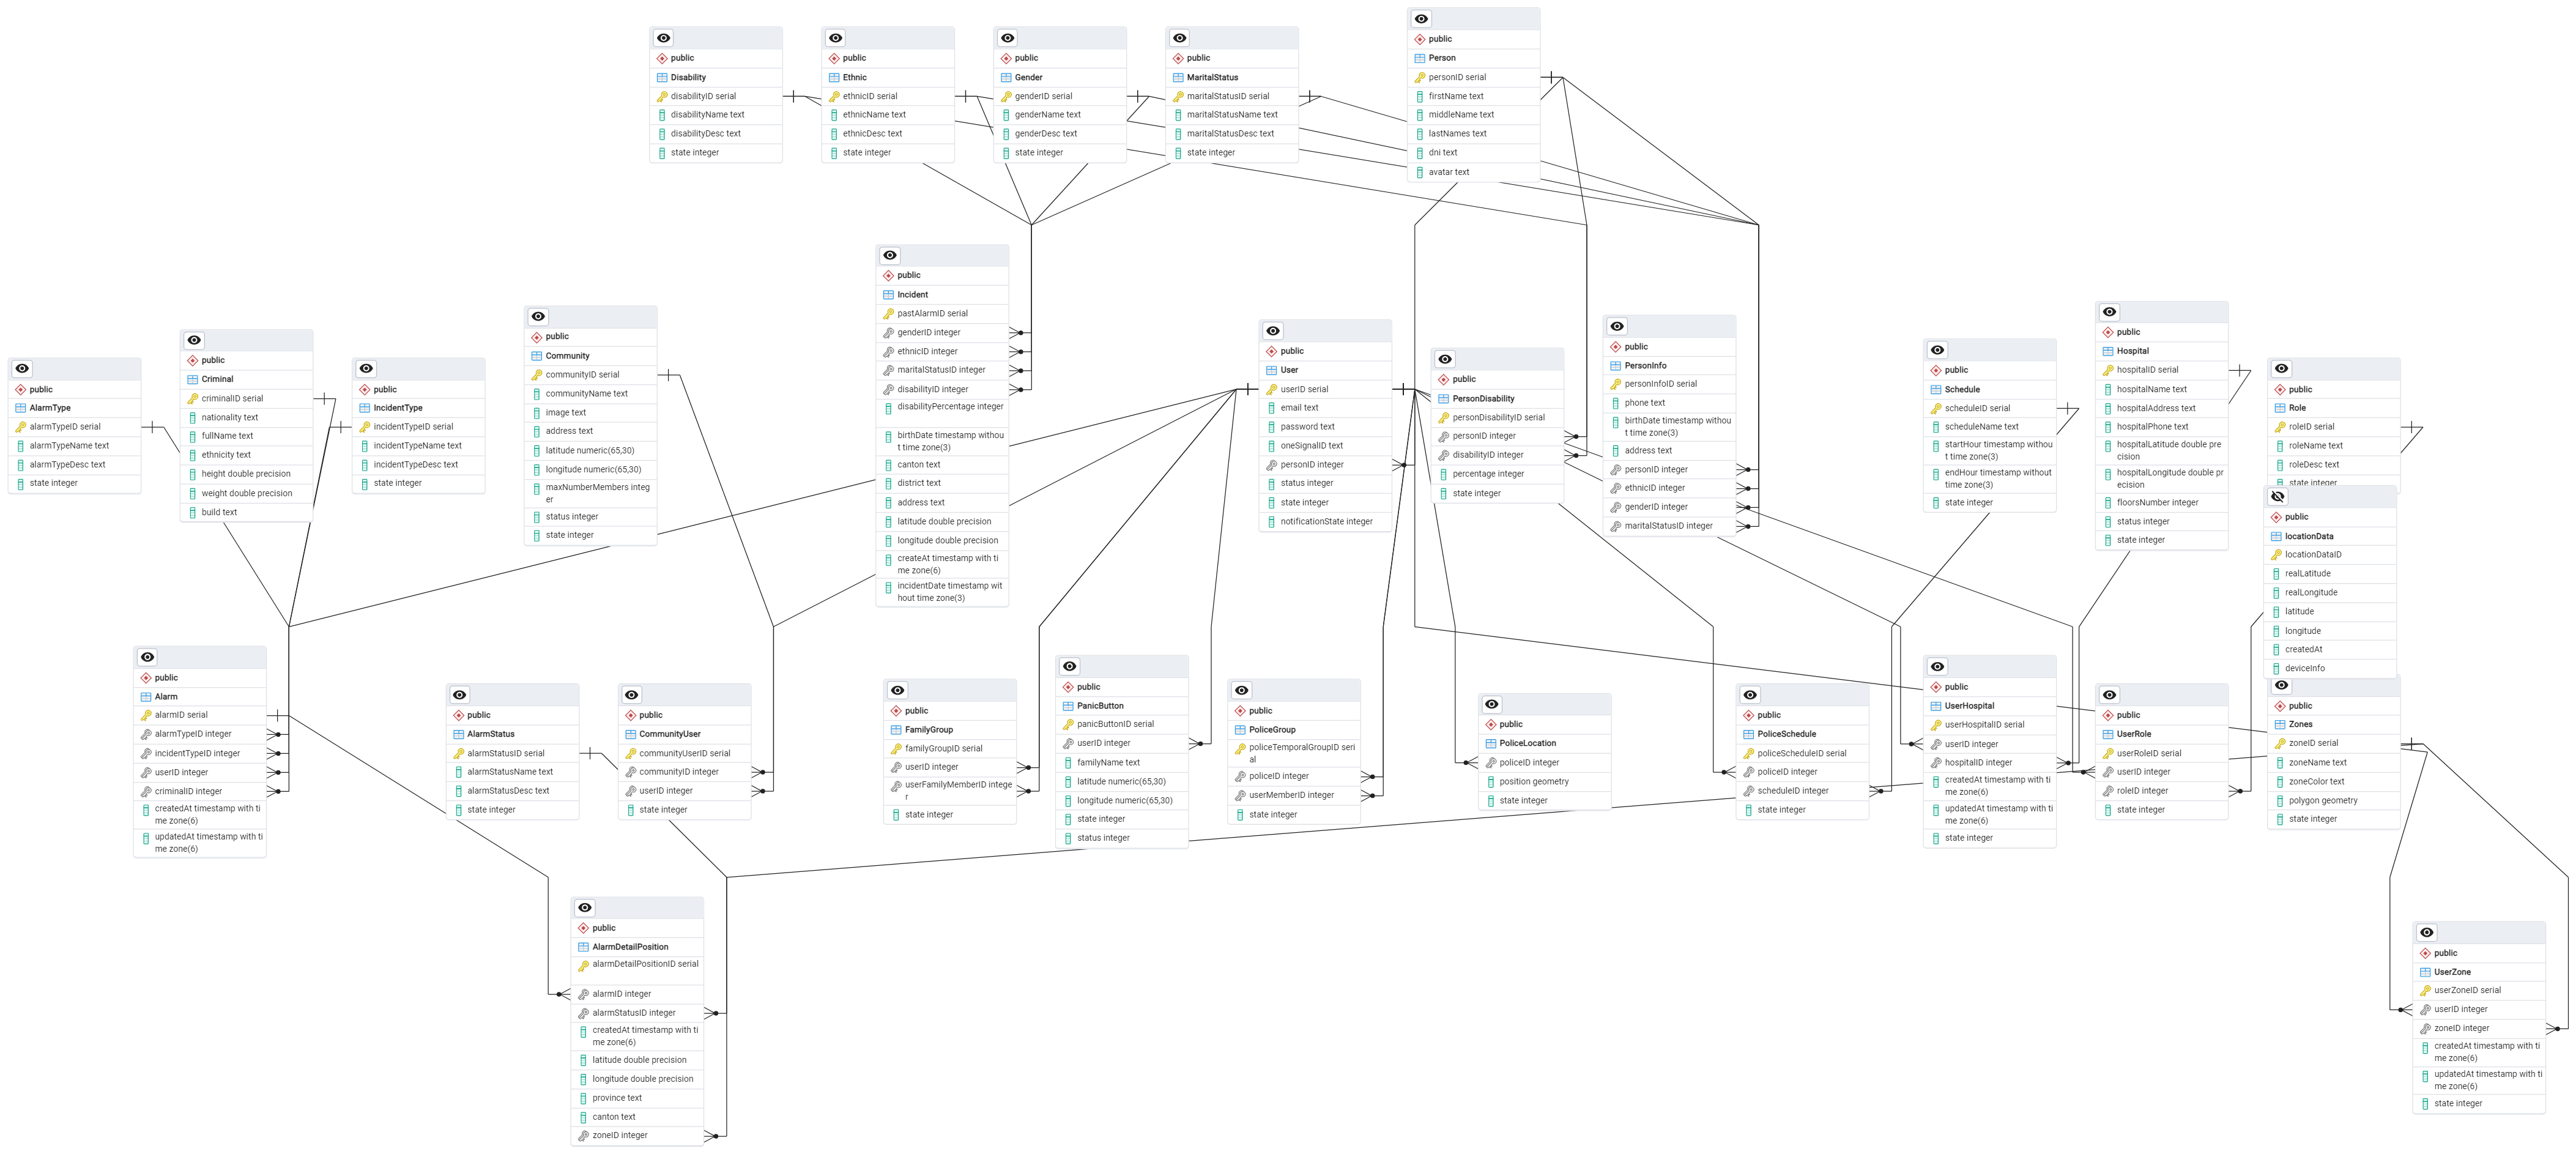
\includegraphics[width=1.7\textwidth]{chapters/III-resultados-y-discusion/resources/images/migracion-base-datos.png}
        \caption{Migración de la base de datos con PrismaJS.}
        \label{fig:migracion-base-datos}
    \end{figure}
\end{landscape}

\paragraph{Validación de datos}
Para la validación de datos en la API, se utilizó la librería class-validator, la cual permite definir reglas de validación mediante
decoradores en las clases de los modelos de datos. Estos decoradores se encargan de validar los datos de entrada en las solicitudes
realizadas a la API, como se muestra en el Anexo \ref{apendix:validacion-datos-api}.

\paragraph{Envío de correos electrónicos}
Para el envío de correos electrónicos en la API se utilizo la librería de nest mailer, la cual trabaja sobre la librería nodemailer
para el envío de correos electrónicos. Para la configuración del servicio de envío de correos se utilizo el SMTP (Simple Mail Transfer
Protocol) de Gmail, este permite enviar correos electrónicos utilizando la cuenta de Gmail del usuario administrador, como se muestra
en el Anexo \ref{apendix:envio-correos-api}.
\bigbreak

Para plantilla de correo electrónico se utilizó el sistema de plantillas de handlebars, el cual permite generar HTML dinámico a partir
de un archivo de plantilla y datos de contexto en formato JSON. En el Anexo \ref{apendix:plantilla-correo-api} se muestra la plantilla
de correo electrónico utilizada para recuperar la contraseña de un usuario.

\paragraph{Configuracion y uso del servicio de almacenamiento de imágenes}
Para el almacenamiento de imágenes en la API se utilizó el servicio de Cloudinary, el cual permite almacenar y gestionar imágenes en la nube.
Cloudinary provee una librería para NodeJS que facilita la subida de imágenes, para la configuración se requiere obtener una api key, api secret
y cloud name, como se muestra en el Anexo \ref{apendix:configuracion-cloudinary-api}.
\bigbreak

Una vez configurado el servicio de Cloudinary, se procedió a implementar la subida de imágenes en la API. Para ello, se creó un servicio
que abstrae la lógica de la librería de Cloudinary y permite subir imágenes a Cloudinary y obtener la URL de la imagen subida, como se
muestra en el Anexo \ref{apendix:subida-imagenes-api}. Este servicio se inyectó en el controlador de la API y se utilizó en el endpoint
de creación de usuarios para subir la fotografía de perfil del usuario, como se muestra en el Anexo \ref{apendix:subida-imagenes-usuario-api}.

\paragraph{Configuración y uso del servicio de notificaciones push}
Para el envío de notificaciones push en la API, se utilizó el servicio de OneSignal, que permite enviar notificaciones a dispositivos
móviles y navegadores web. OneSignal provee una librería para Node.js que facilita el envío de notificaciones push. Para la configuración,
se requiere obtener una app ID y una API key, como se muestra en el Anexo \ref{apendix:configuracion-onesignal-api}.
\bigbreak

Con la configuración realizada, se procedió a implementar una abstracción del API de la librería de OneSignal en un servicio que proporciona
una instancia del cliente para el envío de notificaciones, como se puede visualizar en el Anexo \ref{apendix:configuracion-onesignal-api}. Este servicio
se inyectó en el controlador del módulo de notificaciones push, en el cual se implementó un endpoint para enviar notificaciones a los miembros
del grupo familiar del usuario y a los policías dentro de la zona de emergencia, como se puede observar en el Anexo \ref{apendix:envio-notificaciones-api}.

\paragraph{Modulos}
NestJS permite organizar la aplicación en módulos, los cuales contienen controladores, servicios y dto (Data Transfer Object). Los módulos se encargan
de importar y exportar los componentes de la aplicación, lo que facilita la reutilización de código y la separación de responsabilidades. En el Anexo
\ref{apendix:modulos-api} se muestra la estructura de los módulos de la API.

\paragraph{Controladores}
Los controladores en NestJS son clases que se encargan de gestionar las solicitudes HTTP y devolver una respuesta al cliente. Cada controlador
contiene una serie de métodos que se corresponden con los diferentes endpoints de la API ademas de los decoradores que definen los permisos de
acceso a los recursos protegidos. En el Anexo \ref{apendix:controladores-api} se muestra la estructura de los controladores de la API.

\paragraph{Servicios}
Los servicios en NestJS son clases que contienen la lógica de negocio de la aplicación y se encargan de interactuar con la base de datos y otros
servicios externos. Los servicios se inyectan en los controladores y otros servicios mediante la inyección de dependencias, lo que permite reutilizar
la lógica de negocio en diferentes partes de la aplicación. En el Anexo \ref{apendix:servicios-api} se muestra la estructura de los servicios de la API.

\paragraph{DTO (Data Transfer Object)}
Los DTO en NestJS son clases que se utilizan para transferir datos entre los controladores y los servicios de la aplicación. Los DTO definen la
estructura de los datos que se envían y reciben en las solicitudes HTTP, lo que facilita la validación de datos y la prevención de errores en la
aplicación. En el Anexo \ref{apendix:dto-api} se muestra la estructura de los DTO de la API.

\paragraph{Docuemntación de la API}
Para la documentación de la API se utilizó la librería Swagger, la cual permite generar una documentación interactiva de la API a partir de los
decoradores y comentarios en el código fuente. La documentación de la API se puede visualizar en la ruta /api-docs, como se muestra en la Figura
\ref{fih:documentacion-api}.

\begin{figure}[H]
    \centering
    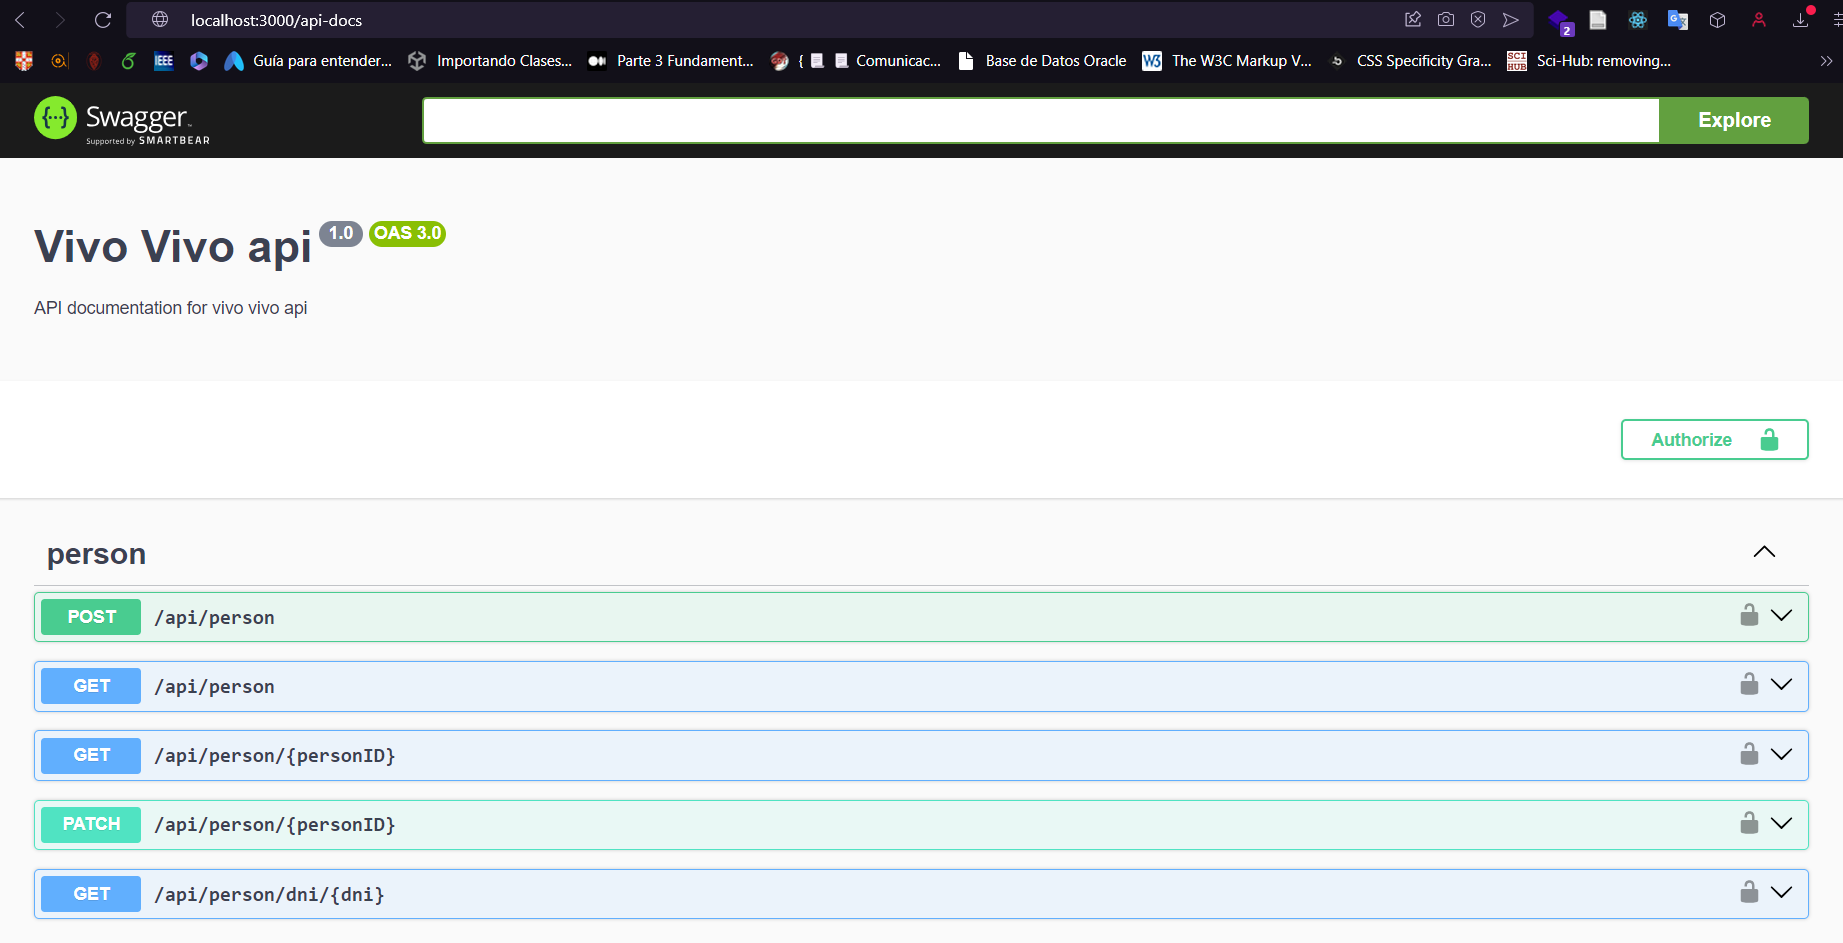
\includegraphics[width=0.8\textwidth]{chapters/III-resultados-y-discusion/resources/images/documentacion-api.png}
    \caption{Documentación de la API con Swagger.}
    \label{fih:documentacion-api}
\end{figure}

\subsubsection{Interfaz de usuario (Frontend)}

\textbf{Sistema web}
\bigbreak

\paragraph{Dependencias del sistema web}
Para crear el proyecto de NextJS se utilizó el comando \mintinline{text}{npx create-next-app@latest}, el cual crea una aplicación de
NextJS con una estructura de carpetas y archivos predefinida. Las dependencias utilizadas en el sistema web se gestionaron mediante
npm y el archivo de configuración package.json. En el Anexo \ref{apendix:dependencias-web} se muestra dependencias utilizadas en el
sistema web.

\paragraph{Configuración de variables de entorno del sistema web}
Para la configuración de las variables de entorno del sistema web se utilizó un archivo .env.local, el cual contiene las propiedades
de la aplicación, como la URL de la API, el api key de Google Maps, la url y secret para la autenticación y la url
para obtener las imágenes de Cloudinary. En el Anexo \ref{apendix:configuracion-env-web} se muestra el archivo .env.local con las
variables de entorno del sistema web.

\paragraph{Configuracion de la aplicación}
En Next.js, la configuración global de la aplicación se realiza mediante Providers y Contexts, los cuales permiten compartir datos y
funcionalidades entre los componentes. En el Anexo \ref{apendix:configuracion-aplicacion-web} se muestra la configuración para los
proveedores de sesión, componentes de UI, notificaciones y gestión de datos en el sistema web.

Las rutas de la aplicación en Next.js se crean mediante el gestor de archivos, el cual permite crear rutas dinámicas y estáticas
siguiendo una estructura "carpeta/page.ts", donde "carpeta" es el nombre de la ruta y "page.ts" es el archivo de la página. En el
Anexo \ref{apendix:rutas-aplicacion-web} se muestra la estructura de las rutas de la aplicación web.

\paragraph{Inicio de sesión}
El inicio de sesión en el sistema web se realiza mediante un formulario en el cual el usuario ingresa su correo electrónico y
contraseña, como se muestra en la Figura \ref{fig:inicio-sesion-web}. Estos campos son validados mediante la librería Zod, la
cual permite definir esquemas de validación para los datos de entrada en los formularios, como se puede observar en el Anexo
\ref{apendix:validacion-datos-web}. Una vez validados los datos, se envía una solicitud POST a la API para autenticar al usuario
y obtener un token JWT, el cual se almacena en la sesión del navegador para mantener la sesión activa, en el Anexo
\ref{apendix:guardar-token-web} se muestra el código para guardar el token en la sesión del navegador.

\begin{figure}[H]
    \centering
    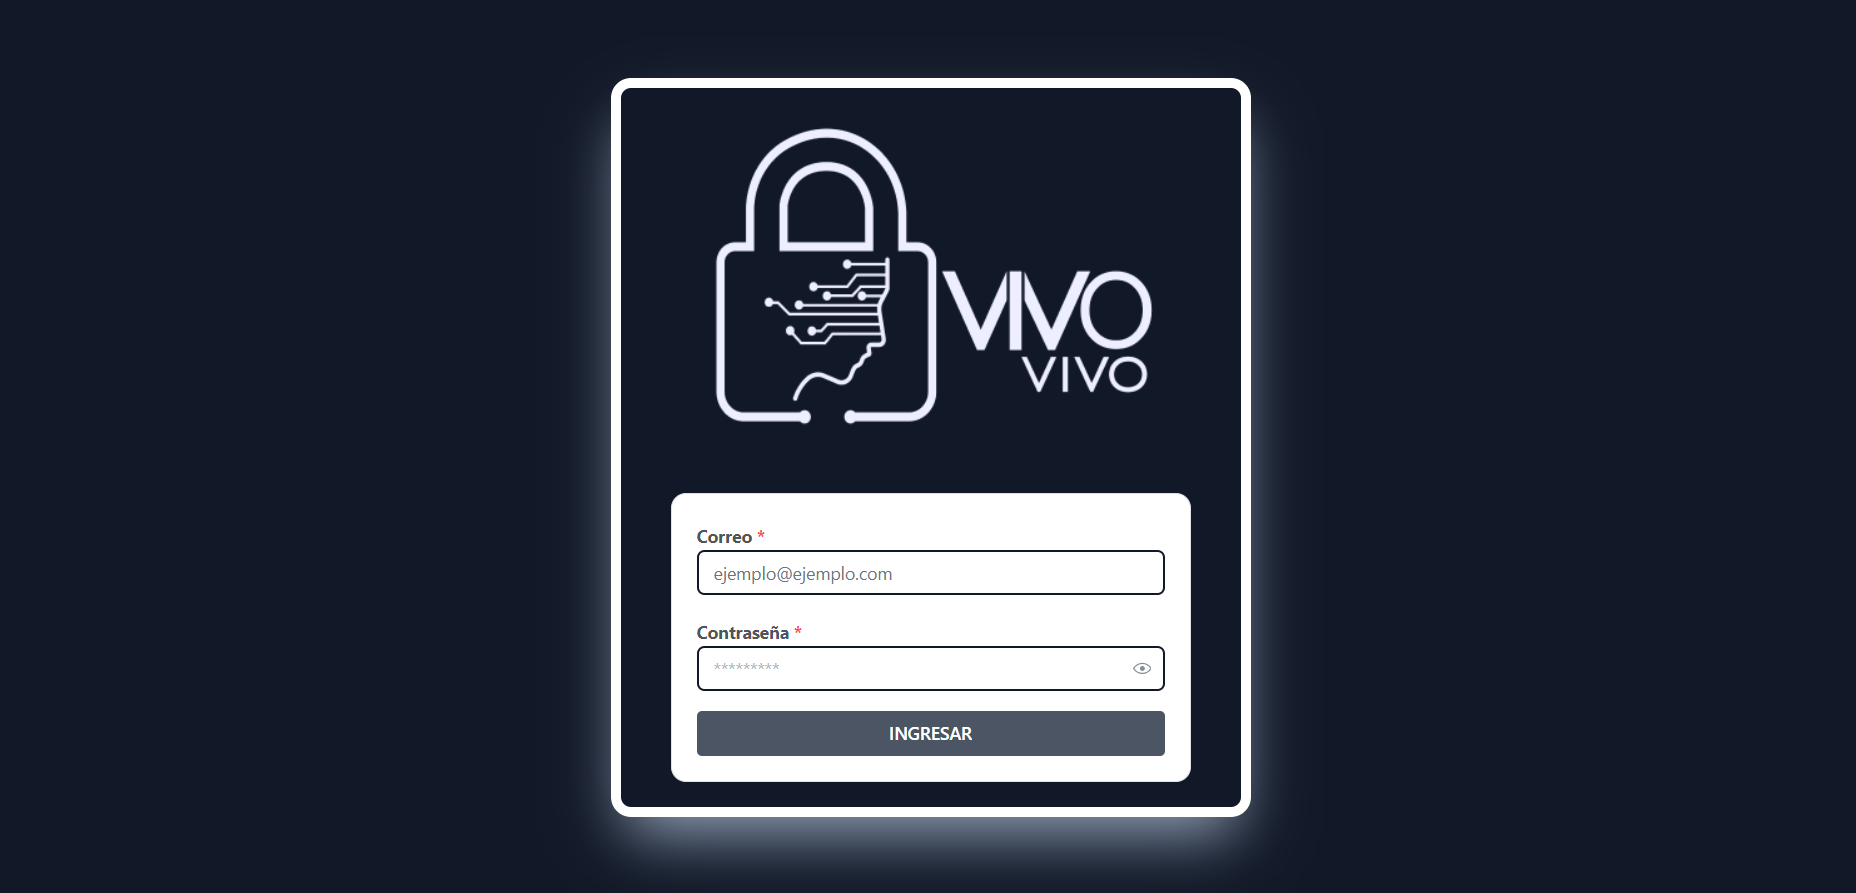
\includegraphics[width=0.8\textwidth]{chapters/III-resultados-y-discusion/resources/images/inicio-sesion-web.png}
    \caption{Inicio de sesión en el sistema web.}
    \label{fig:inicio-sesion-web}
\end{figure}

\paragraph{Menú de usuario}
El menú de usuario en el sistema web permite al usuario administrador acceder a las opciones de la aplicación al hacer clic en
el botón de configuración en la esquina superior derecha de la pantalla. Al hacer esto, se muestra un menú desplegable en el
cual se encuentran las opciones de cambiar contraseña y cerrar sesión, como se muestra en la Figura \ref{fig:menu-usuario-web}.

\begin{figure}[H]
    \centering
    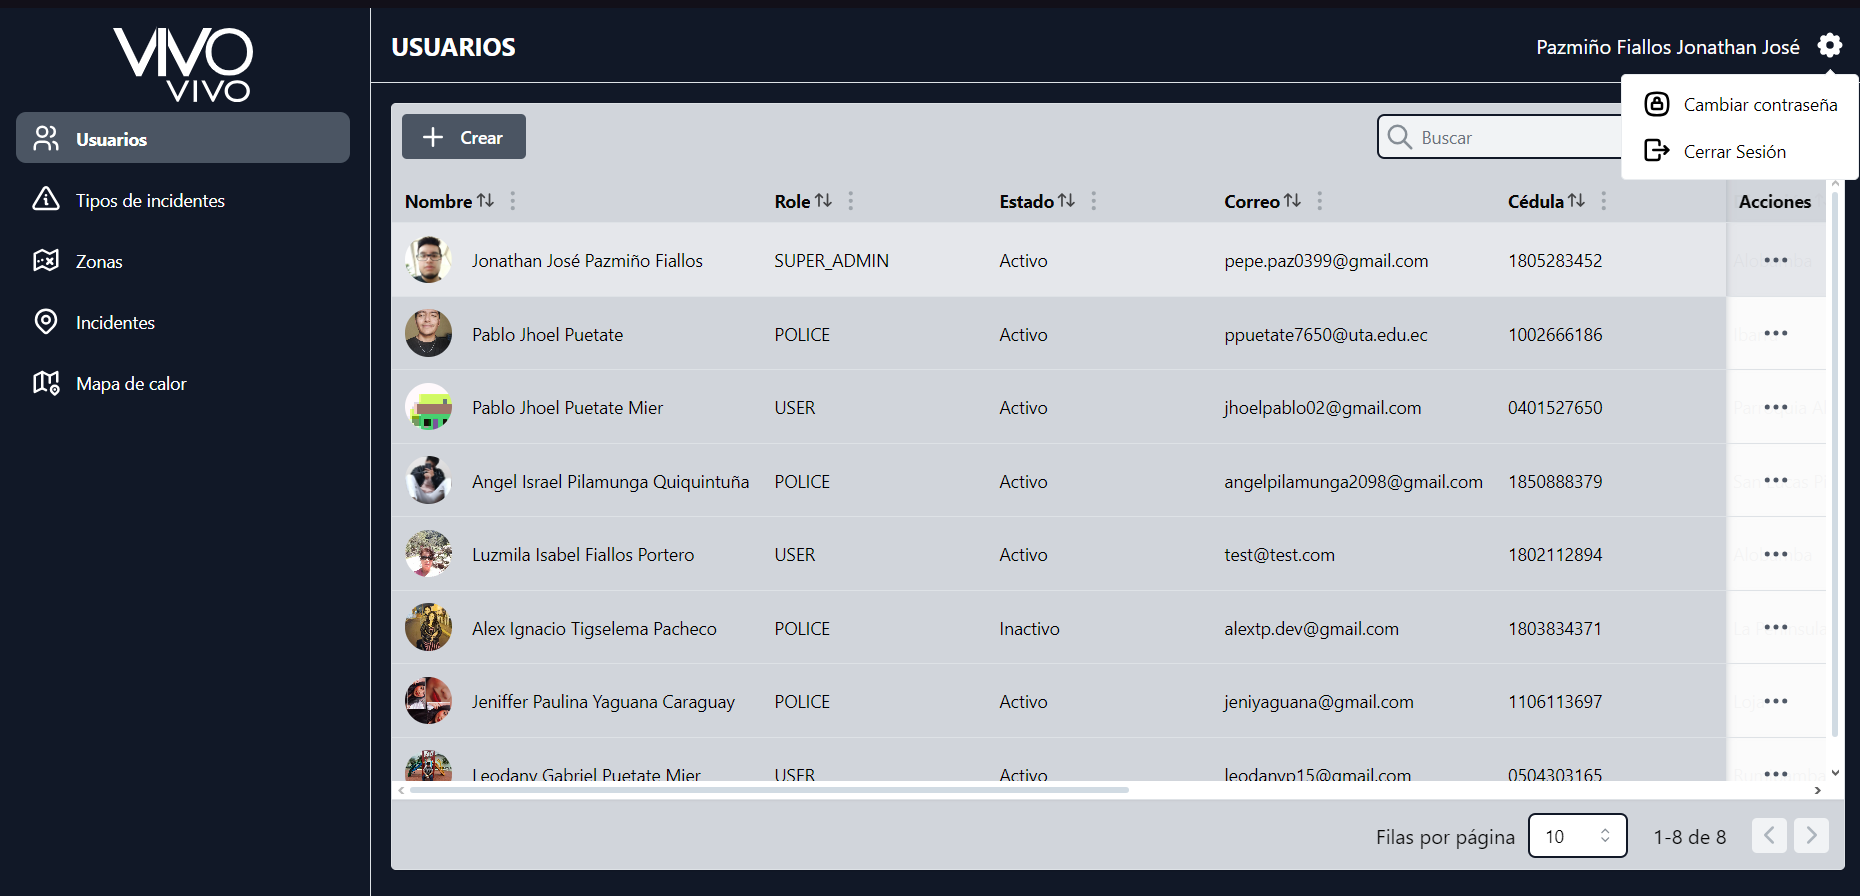
\includegraphics[width=0.8\textwidth]{chapters/III-resultados-y-discusion/resources/images/menu-usuario-web.png}
    \caption{Menú de usuario en el sistema web.}
    \label{fig:menu-usuario-web}
\end{figure}

\paragraph{Gestion de usuarios}
La gestión de usuarios en el sistema web se realiza mediante una tabla de entradas, la cual permite al usuario administrador
visualizar los usuarios registrados en el sistema, como se muestra en la Figura \ref{fig:tabla-usuarios-web}. En esta tabla se
muestran los campos de la información de los usuarios, como la fotografía, nombres, apellidos, correo electrónico, etnia, género,
entre otros. El usuario administrador puede realizar acciones como crear, editar y deshabilitar usuarios, como se puede observar en la Figura
\ref{fig:menu-tabla-usuarios-web}. El formulario de registro de usuarios permite al usuario administrador ingresar la información
necesaria para crear un nuevo usuario, como se puede visualizar en las Figuras \ref{fig:formulario-usuario-web-1} y \ref{fig:formulario-usuario-web-2}.

\begin{figure}[H]
    \centering
    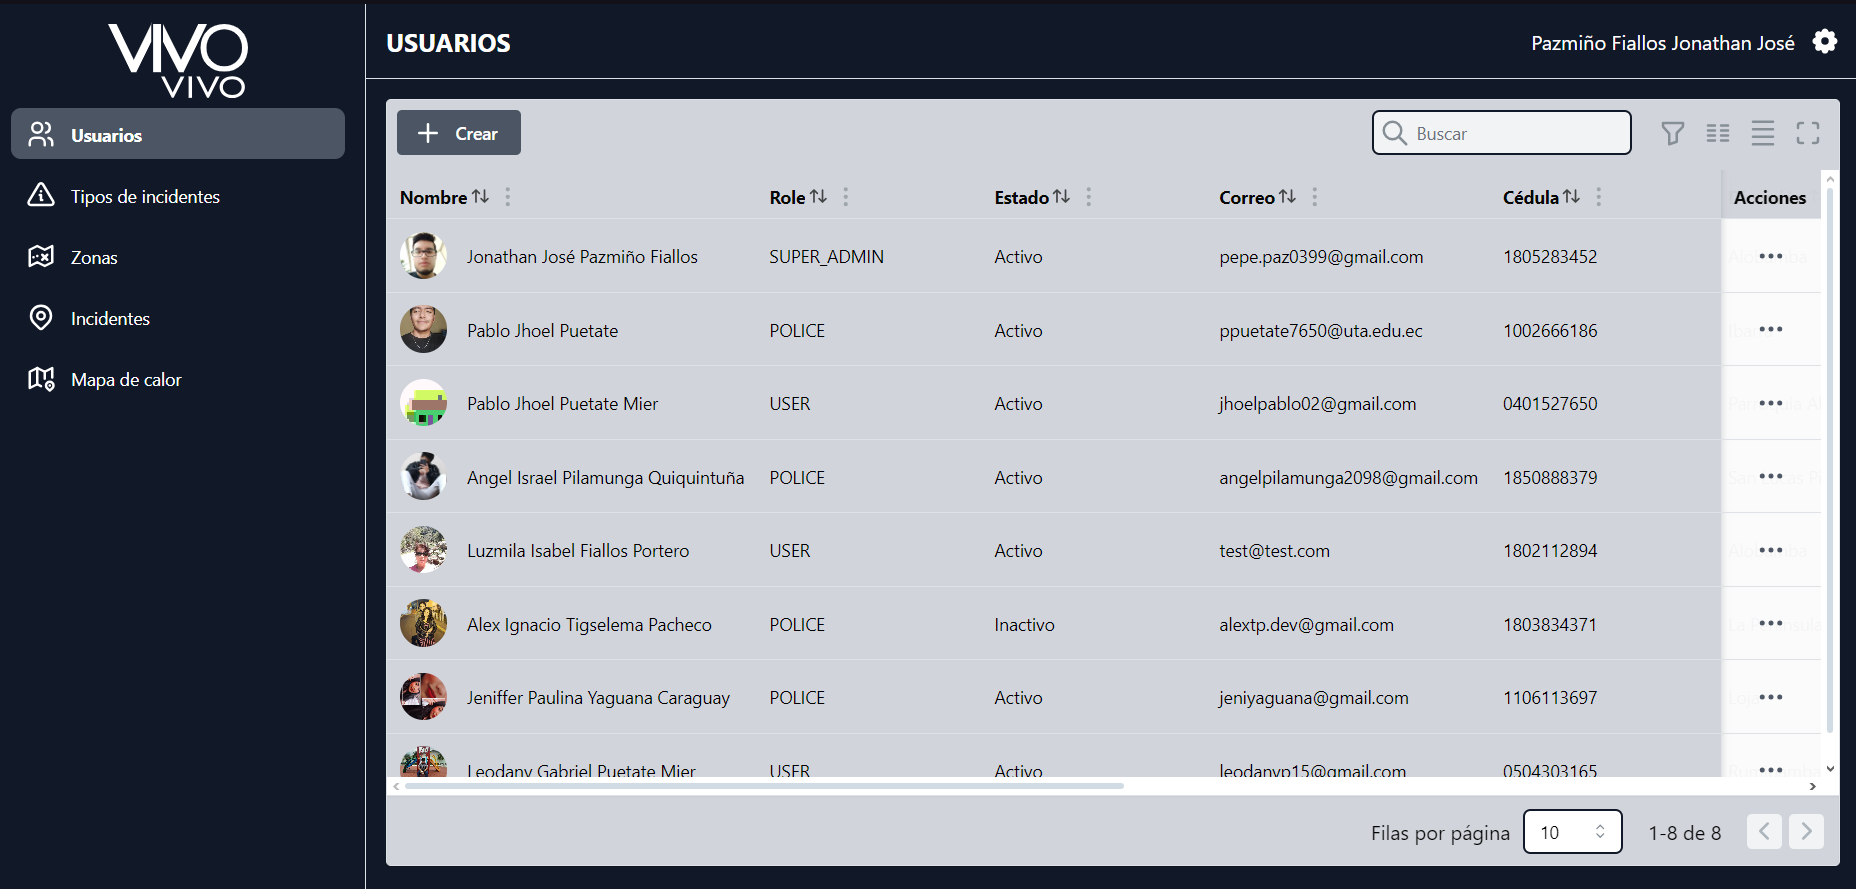
\includegraphics[width=0.8\textwidth]{chapters/III-resultados-y-discusion/resources/images/tabla-usuarios-web.png}
    \caption{Tabla de usuarios en el sistema web.}
    \label{fig:tabla-usuarios-web}
\end{figure}

\begin{figure}[H]
    \centering
    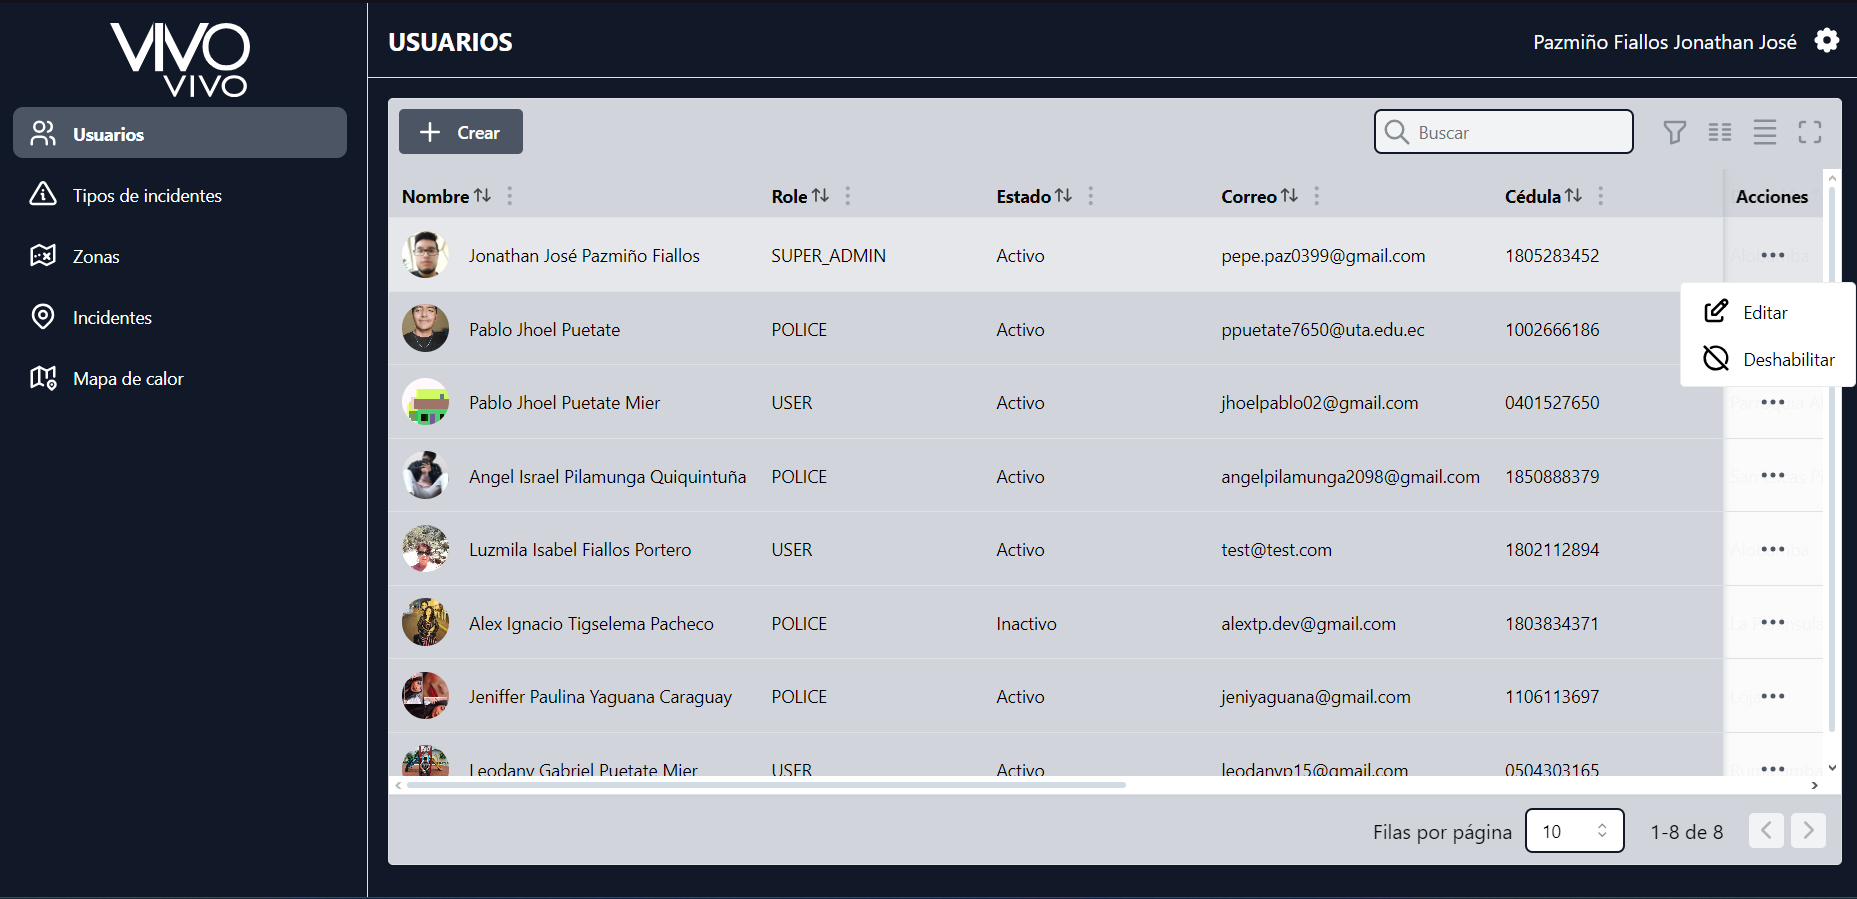
\includegraphics[width=0.8\textwidth]{chapters/III-resultados-y-discusion/resources/images/menu-tabla-usuarios-web.png}
    \caption{Menú de opciones de la tabla de usuarios en el sistema web.}
    \label{fig:menu-tabla-usuarios-web}
\end{figure}

\begin{figure}[H]
    \centering
    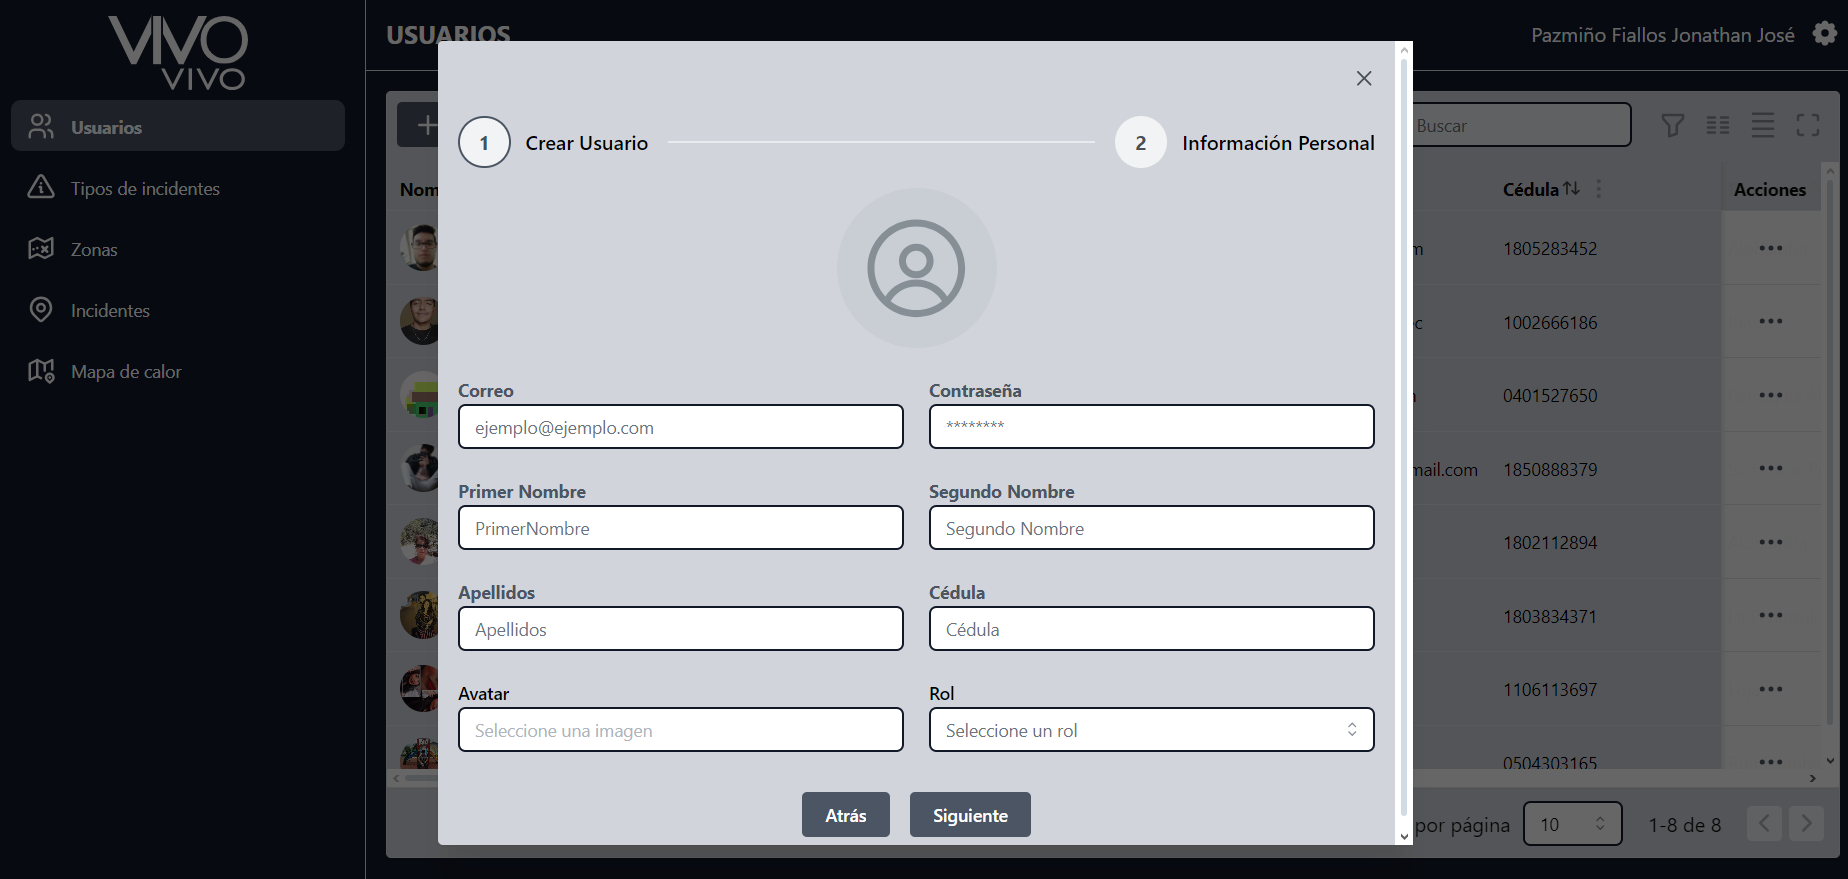
\includegraphics[width=0.8\textwidth]{chapters/III-resultados-y-discusion/resources/images/formulario-usuario-web-1.png}
    \caption{Formulario para crear/editar usuarios en el sistema web (Parte 1).}
    \label{fig:formulario-usuario-web-1}
\end{figure}

\begin{figure}[H]
    \centering
    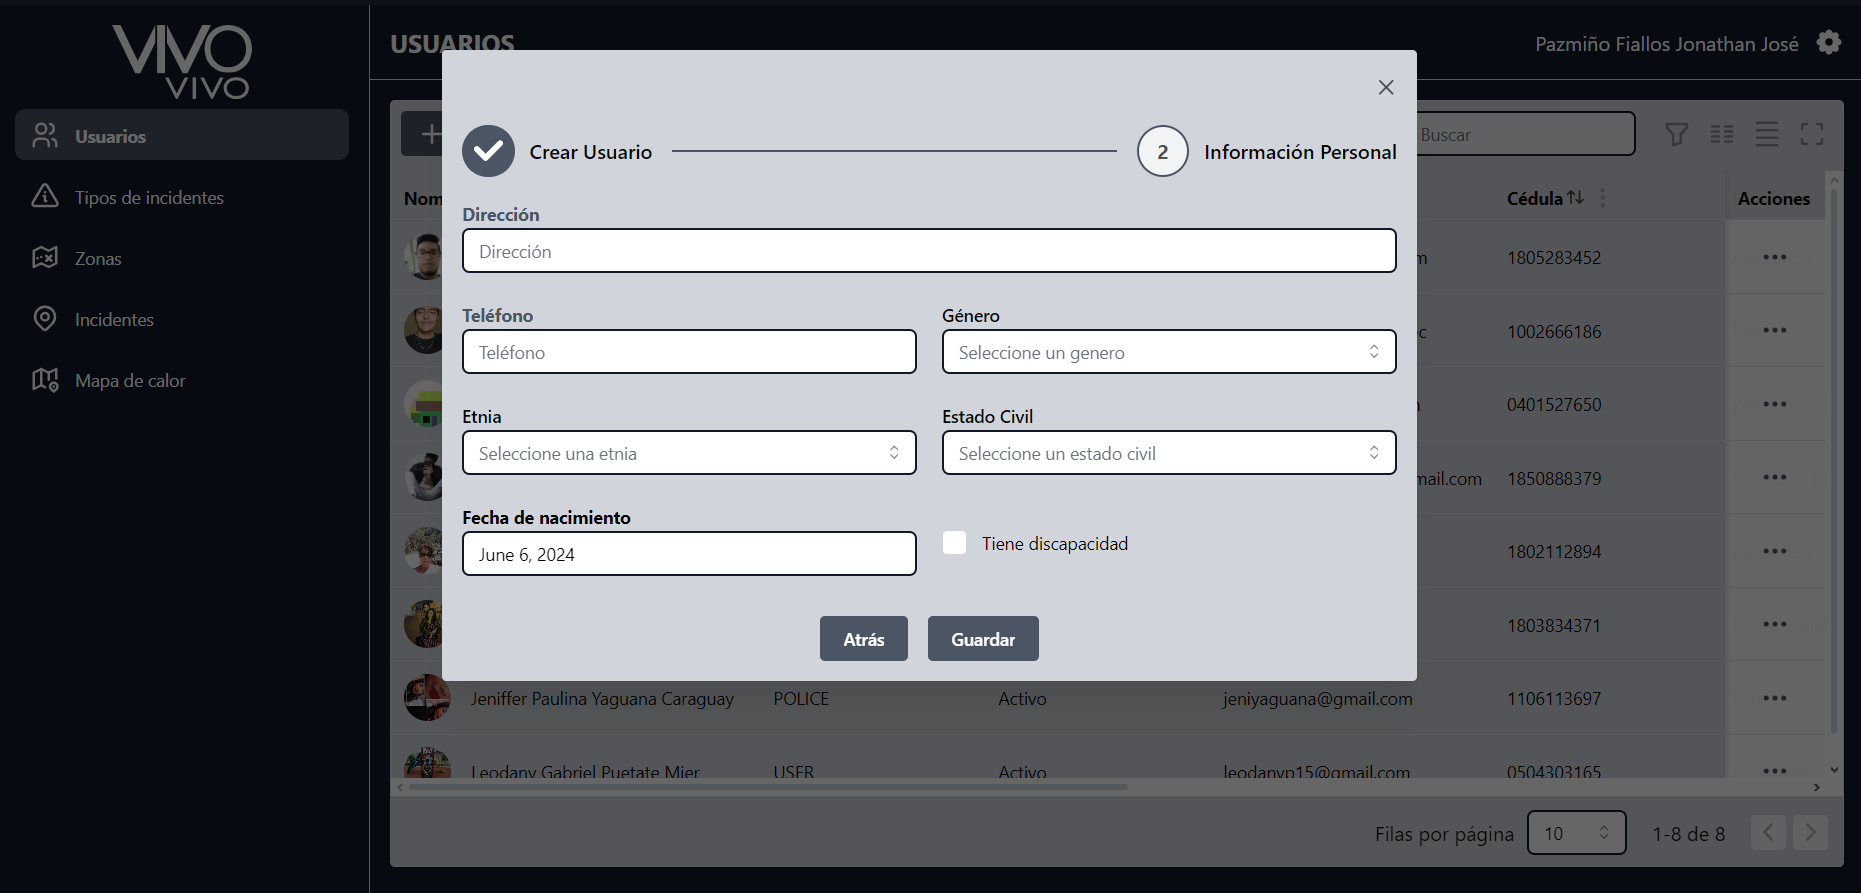
\includegraphics[width=0.8\textwidth]{chapters/III-resultados-y-discusion/resources/images/formulario-usuario-web-2.png}
    \caption{Formulario para crear/editar usuarios en el sistema web (Parte 2).}
    \label{fig:formulario-usuario-web-2}
\end{figure}

La tabla de gestión de usuarios cuenta con varios filtros de búsqueda, los cuales permiten al usuario administrador buscar usuarios por
columnas especificas o por un filtro general, como se muestra en la Figura \ref{fig:filtros-tabla-usuarios-web}.

\begin{figure}[H]
    \centering
    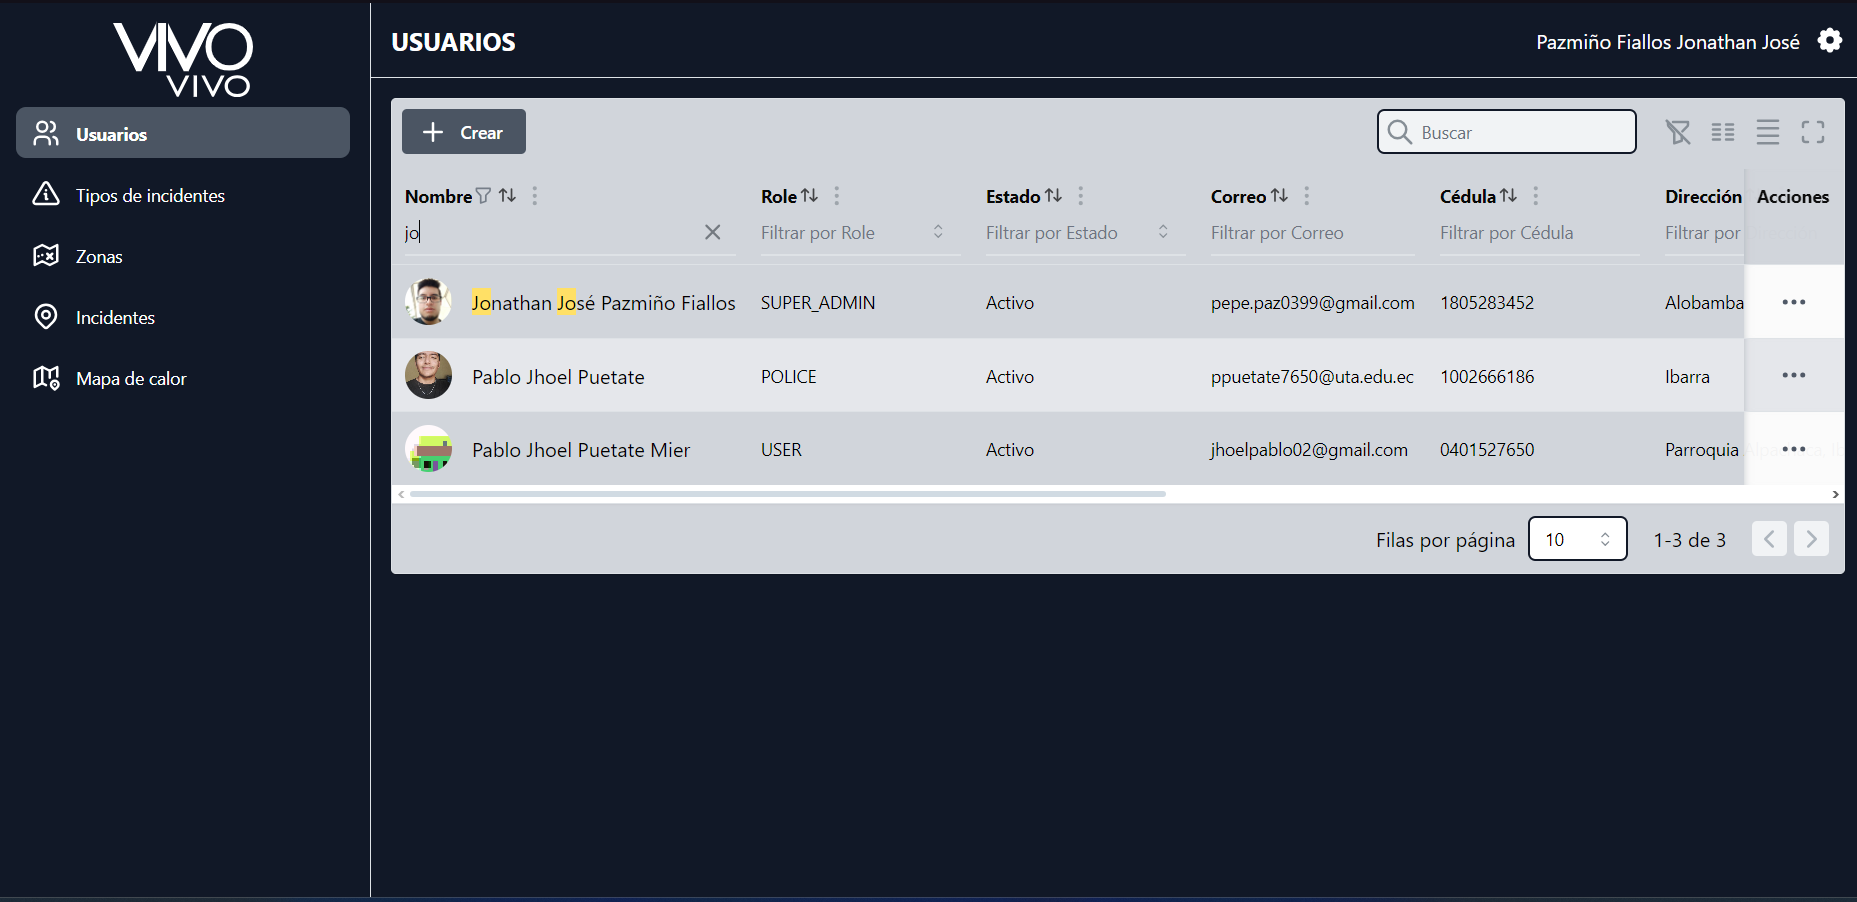
\includegraphics[width=0.8\textwidth]{chapters/III-resultados-y-discusion/resources/images/filtros-tabla-usuarios-web.png}
    \caption{Filtros de búsqueda en la tabla de usuarios en el sistema web.}
    \label{fig:filtros-tabla-usuarios-web}
\end{figure}

\paragraph{Gestión de tipos de incidentes}
La gestión de tipos de incidentes en el sistema web se realiza mediante una tabla de entradas, en la cual el usuario administrador
puede visualizar los tipos de incidentes registrados en el sistema, como se muestra en la Figura \ref{fig:tabla-tipos-incidentes-web}.
En esta tabla se muestran los campos de la información de los tipos de incidentes, como el nombre, descripción y estado. El usuario
administrador puede realizar acciones como crear, editar y deshabilitar tipos de incidentes, como se puede observar en la Figura
\ref{fig:menu-tabla-tipos-incidentes-web}. El formulario de registro de tipos de incidentes permite al usuario administrador ingresar
la información necesaria para crear un nuevo tipo de incidente, como se puede visualizar en la Figura \ref{fig:formulario-tipo-incidente-web}

\begin{figure}[H]
    \centering
    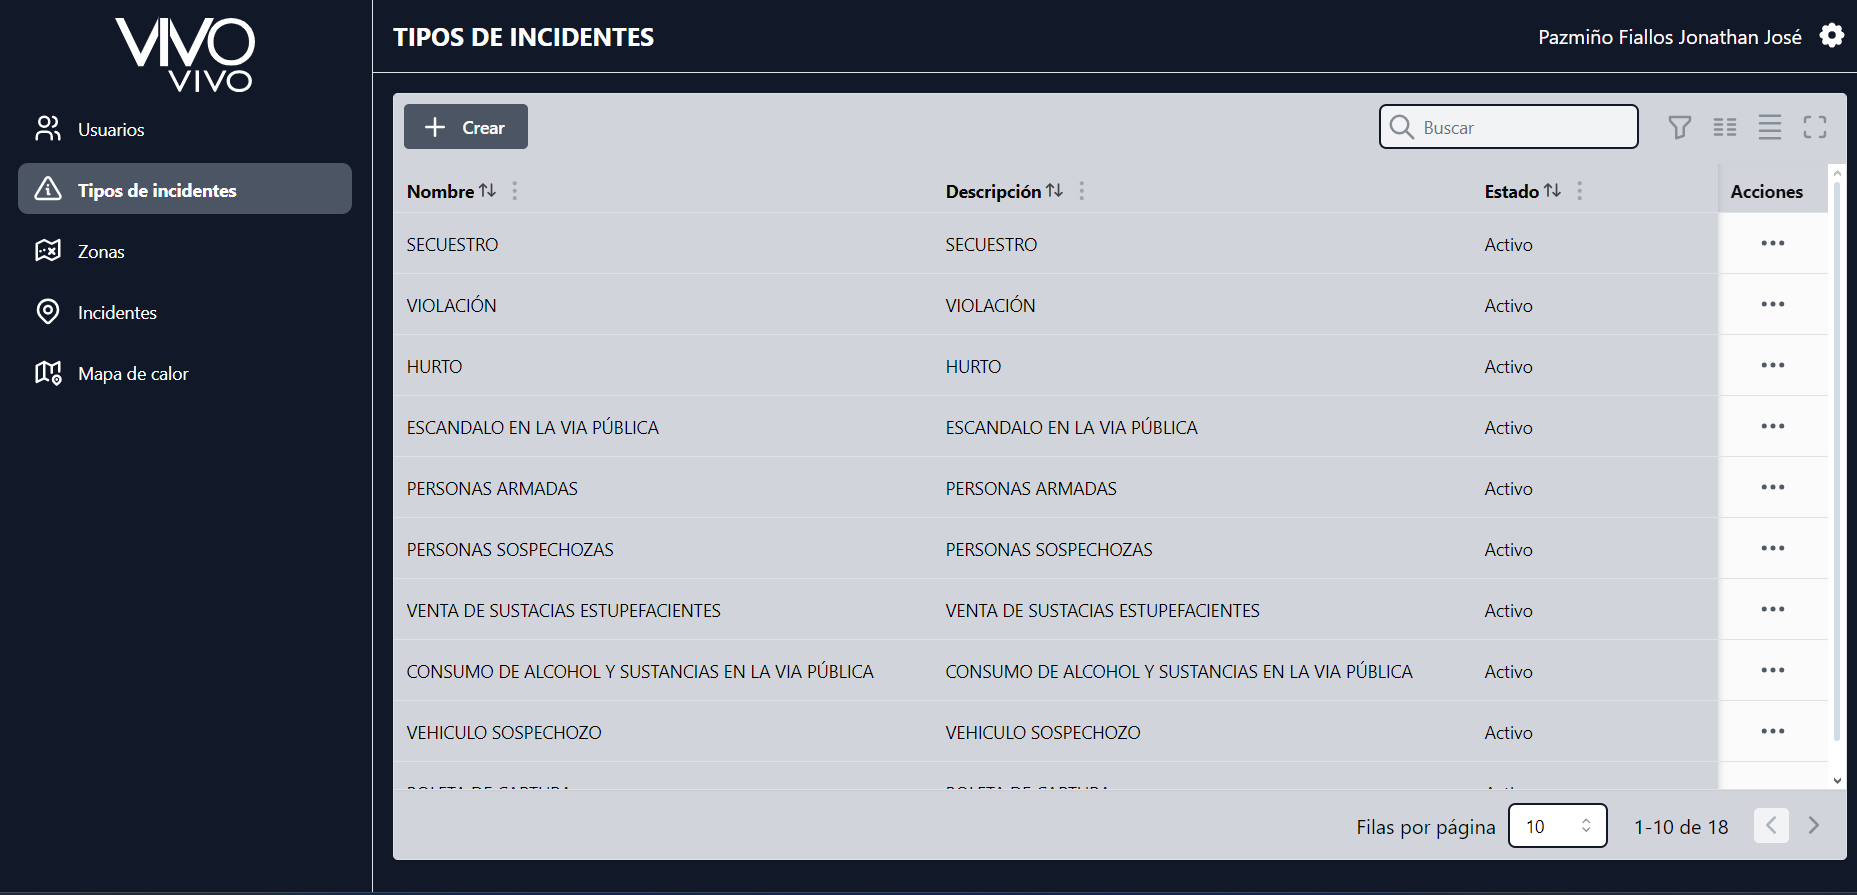
\includegraphics[width=0.8\textwidth]{chapters/III-resultados-y-discusion/resources/images/tabla-tipos-incidentes-web.png}
    \caption{Tabla de tipos de incidentes en el sistema web.}
    \label{fig:tabla-tipos-incidentes-web}
\end{figure}

\begin{figure}[H]
    \centering
    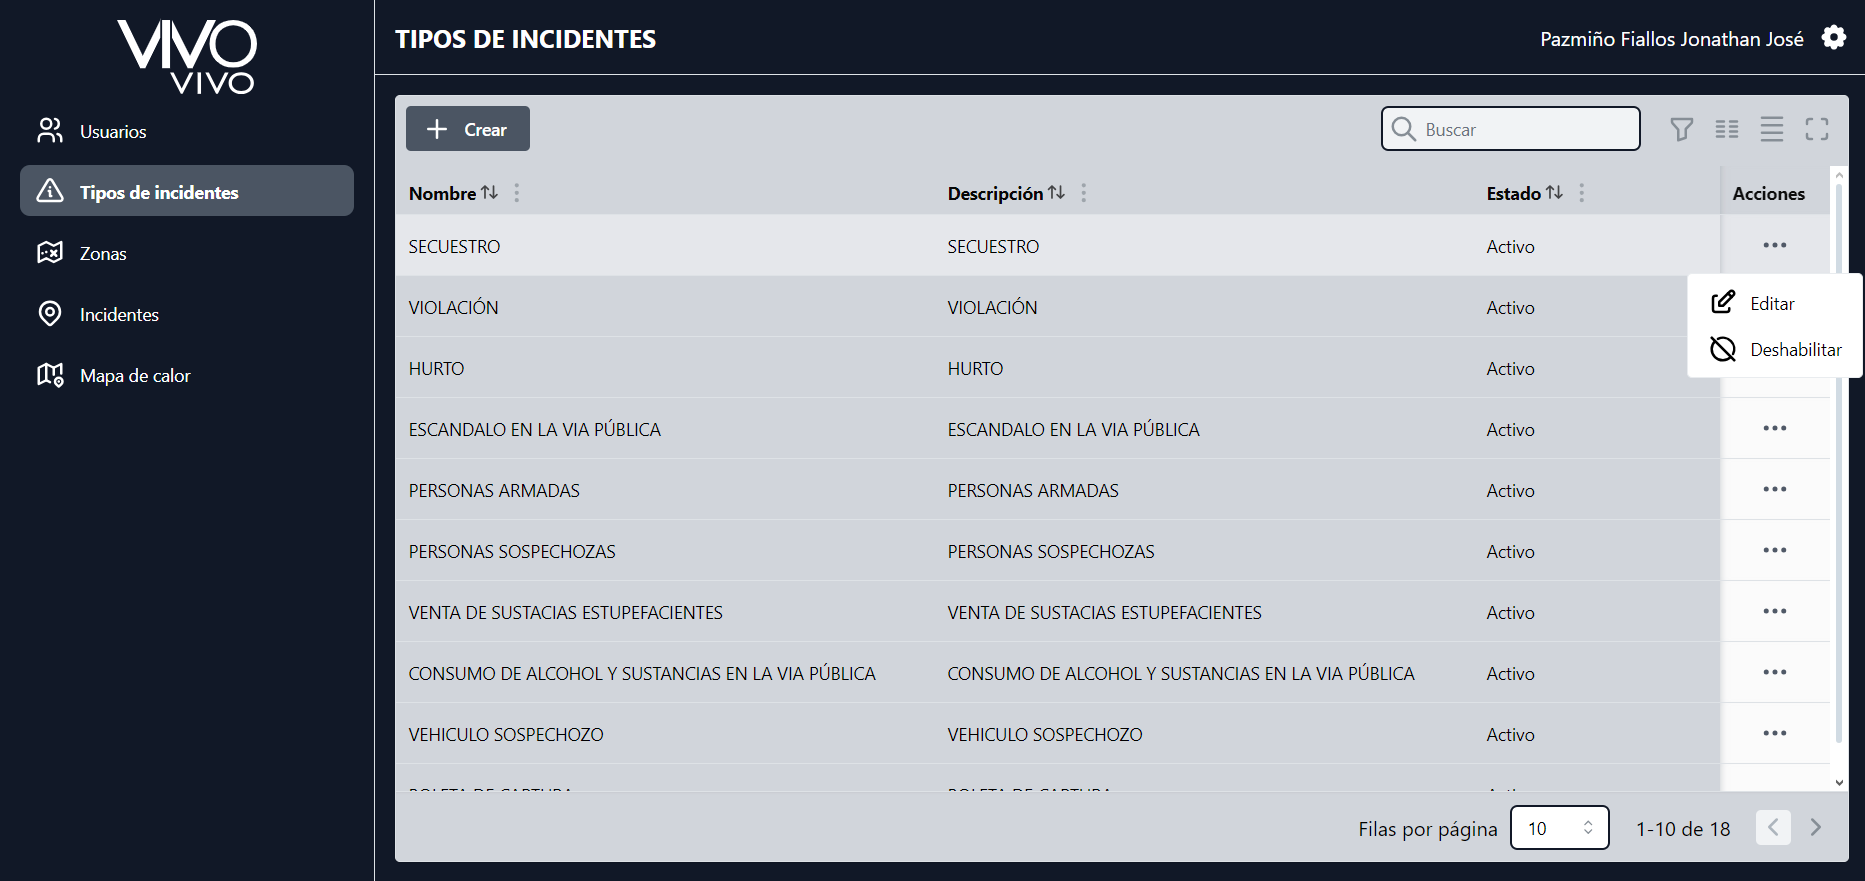
\includegraphics[width=0.8\textwidth]{chapters/III-resultados-y-discusion/resources/images/menu-tabla-tipos-incidentes-web.png}
    \caption{Menú de opciones de la tabla de tipos de incidentes en el sistema web.}
    \label{fig:menu-tabla-tipos-incidentes-web}
\end{figure}

\begin{figure}[H]
    \centering
    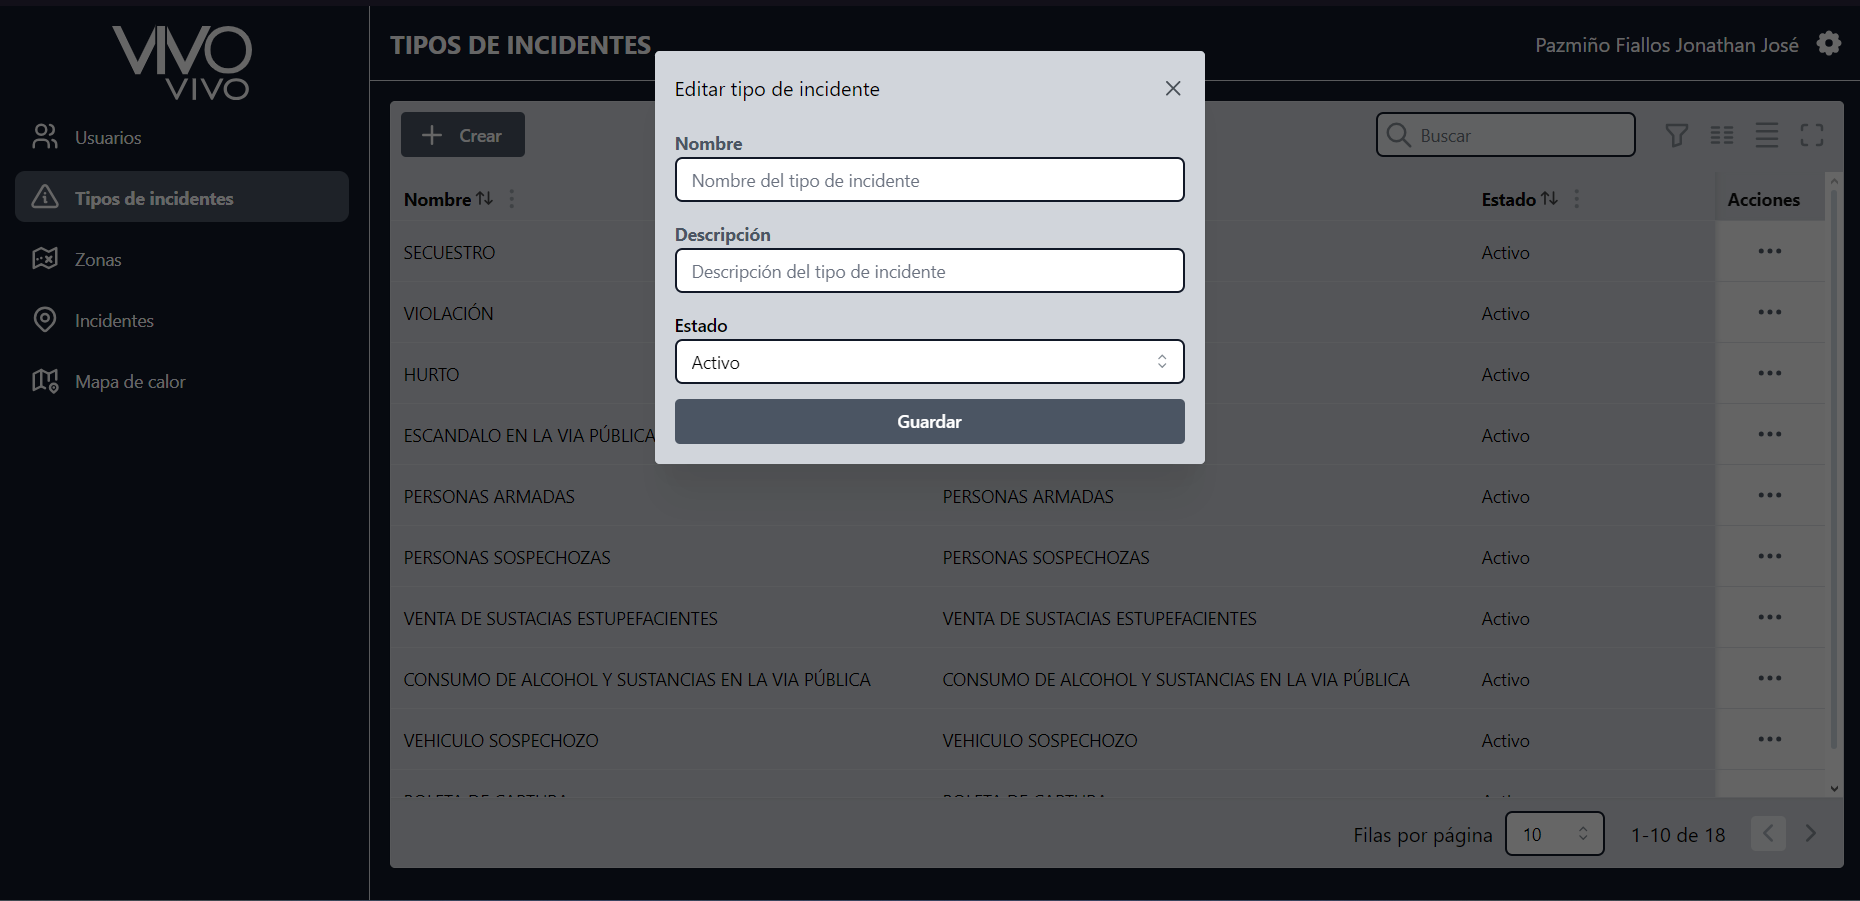
\includegraphics[width=0.8\textwidth]{chapters/III-resultados-y-discusion/resources/images/formulario-tipo-incidente-web.png}
    \caption{Formulario para crear/editar tipos de incidentes en el sistema web.}
    \label{fig:formulario-tipo-incidente-web}
\end{figure}

La tabla de gestión de tipos de incidentes cuenta con varios filtros de búsqueda, los cuales permiten al usuario administrador buscar
tipos de incidentes por columnas especificas o por un filtro general, como se muestra en la Figura \ref{fig:filtros-tabla-tipos-incidentes-web}.

\begin{figure}[H]
    \centering
    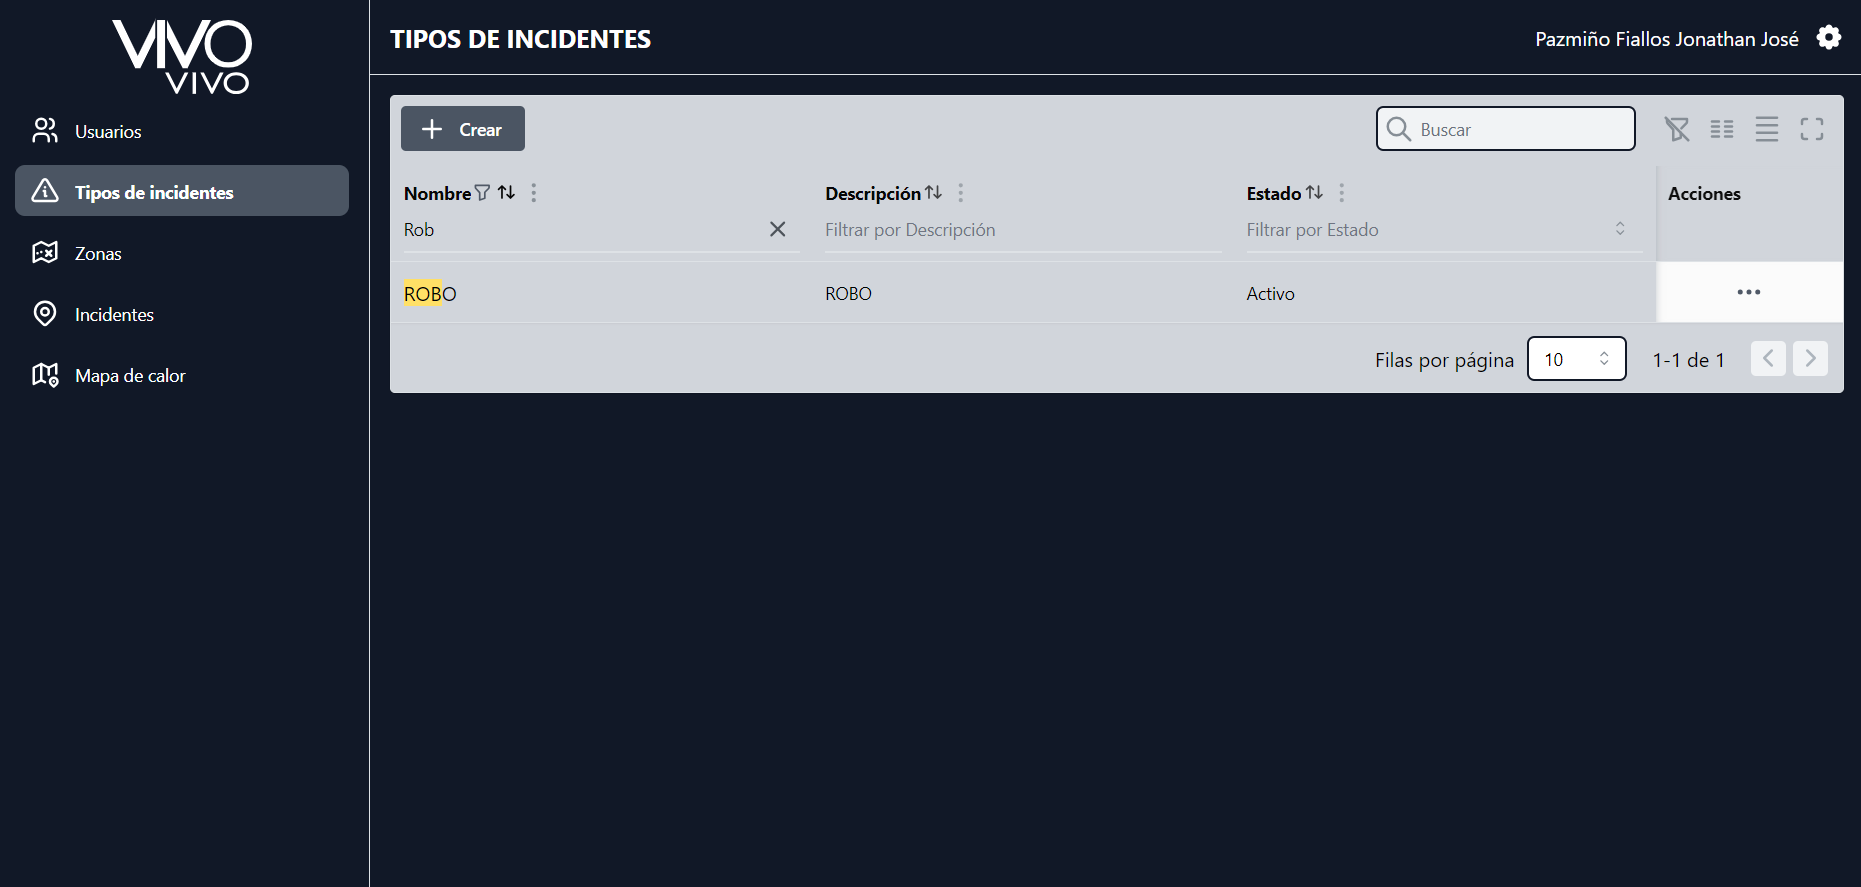
\includegraphics[width=0.8\textwidth]{chapters/III-resultados-y-discusion/resources/images/filtros-tabla-tipos-incidentes-web.png}
    \caption{Filtros de búsqueda en la tabla de tipos de incidentes en el sistema web.}
    \label{fig:filtros-tabla-tipos-incidentes-web}
\end{figure}

\paragraph{Gestión de zonas de vigilancia}

Claro, aquí tienes el texto corregido:

La gestión de zonas de vigilancia en el sistema web se realiza por medio de un mapa interactivo, en el cual el usuario administrador
puede visualizar las zonas de vigilancia mediante polígonos, como se muestra en la Figura \ref{fig:mapa-zonas-vigilancia-web}.
El usuario administrador puede realizar acciones como crear, editar y deshabilitar zonas de vigilancia, como se puede observar en la Figura
\ref{fig:menu-mapa-zonas-vigilancia-web}. El formulario de registro de zonas de vigilancia permite al usuario administrador dibujar
un polígono en el mapa para definir una zona de vigilancia, como se puede visualizar en la Figura \ref{fig:formulario-zona-vigilancia-web}.
Además, el usuario administrador podrá asignar policías a las zonas de vigilancia, como se muestra en la Figura
\ref{fig:asignar-policias-zona-vigilancia-web}.

\begin{figure}[H]
    \centering
    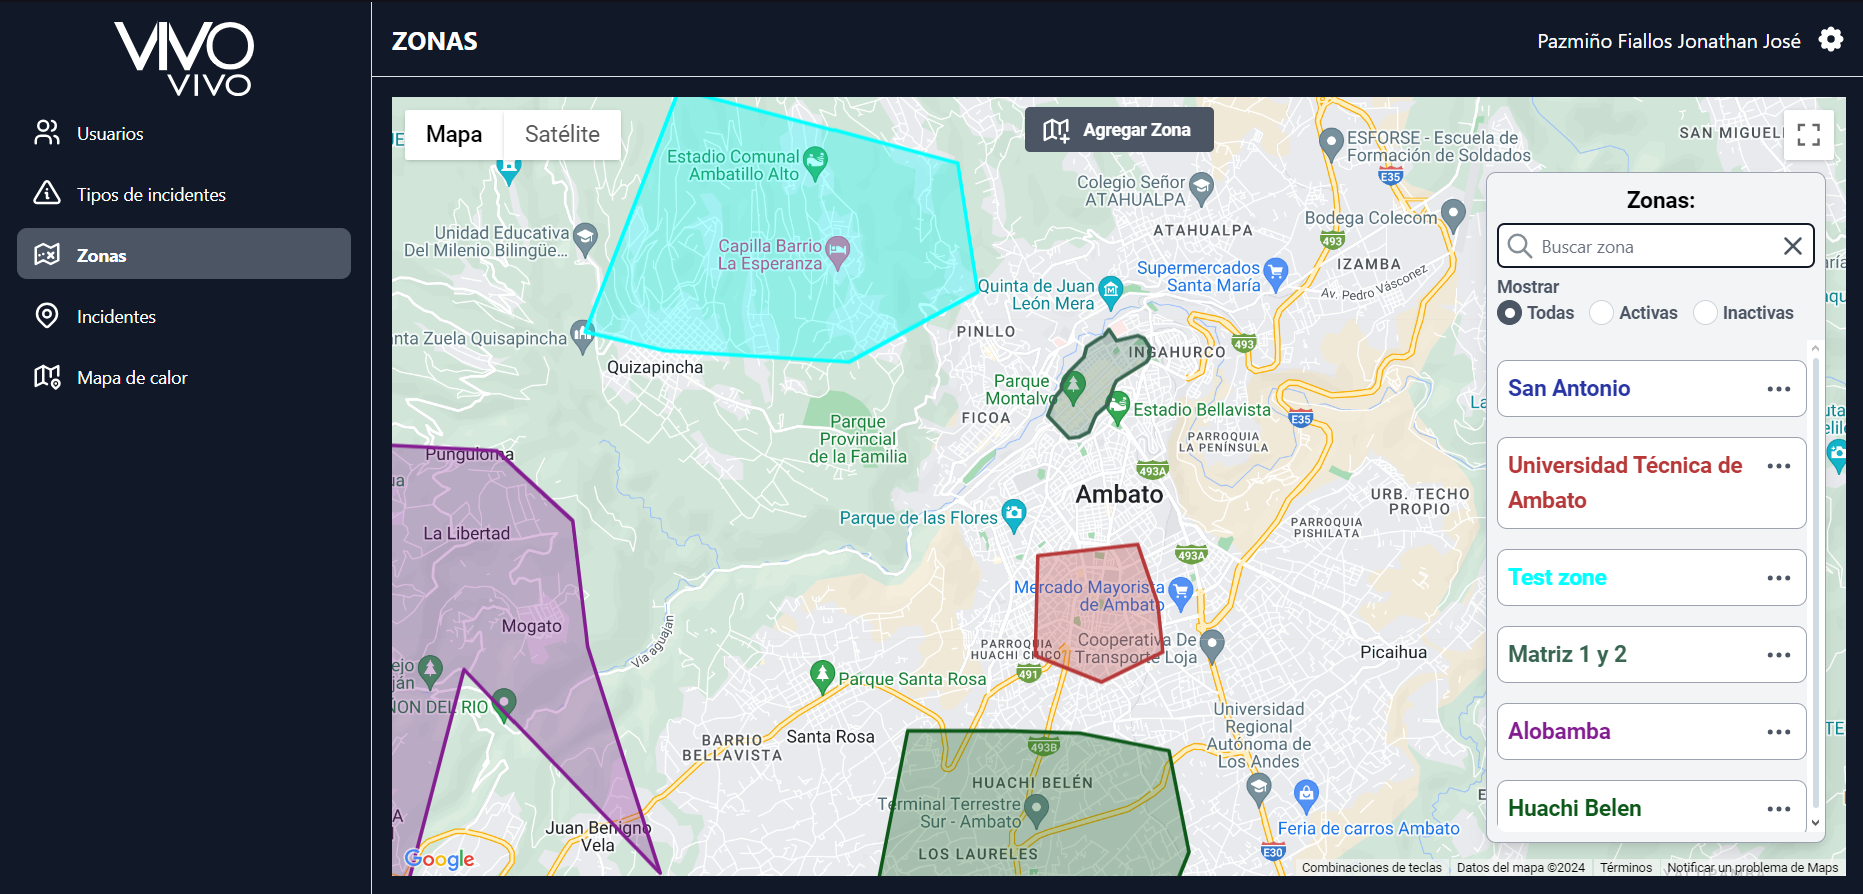
\includegraphics[width=0.8\textwidth]{chapters/III-resultados-y-discusion/resources/images/mapa-zonas-vigilancia-web.png}
    \caption{Mapa de zonas de vigilancia en el sistema web.}
    \label{fig:mapa-zonas-vigilancia-web}
\end{figure}

\begin{figure}[H]
    \centering
    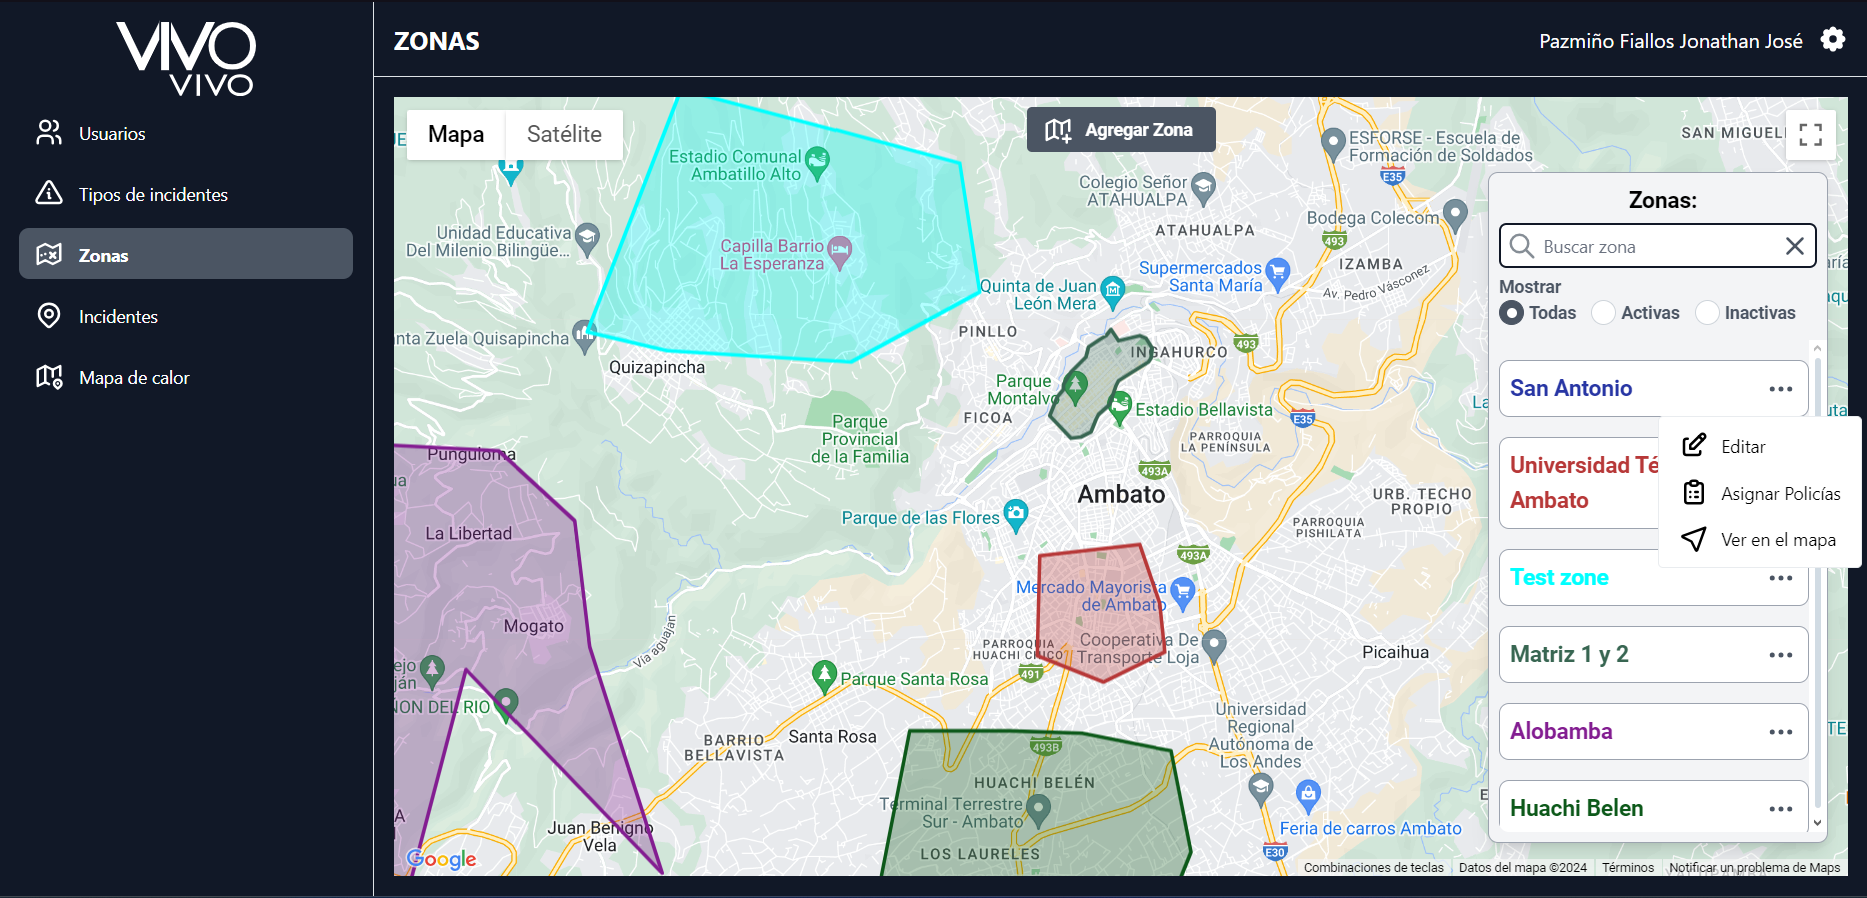
\includegraphics[width=0.8\textwidth]{chapters/III-resultados-y-discusion/resources/images/menu-mapa-zonas-vigilancia-web.png}
    \caption{Menú de opciones del mapa de zonas de vigilancia en el sistema web.}
    \label{fig:menu-mapa-zonas-vigilancia-web}
\end{figure}

\begin{figure}[H]
    \centering
    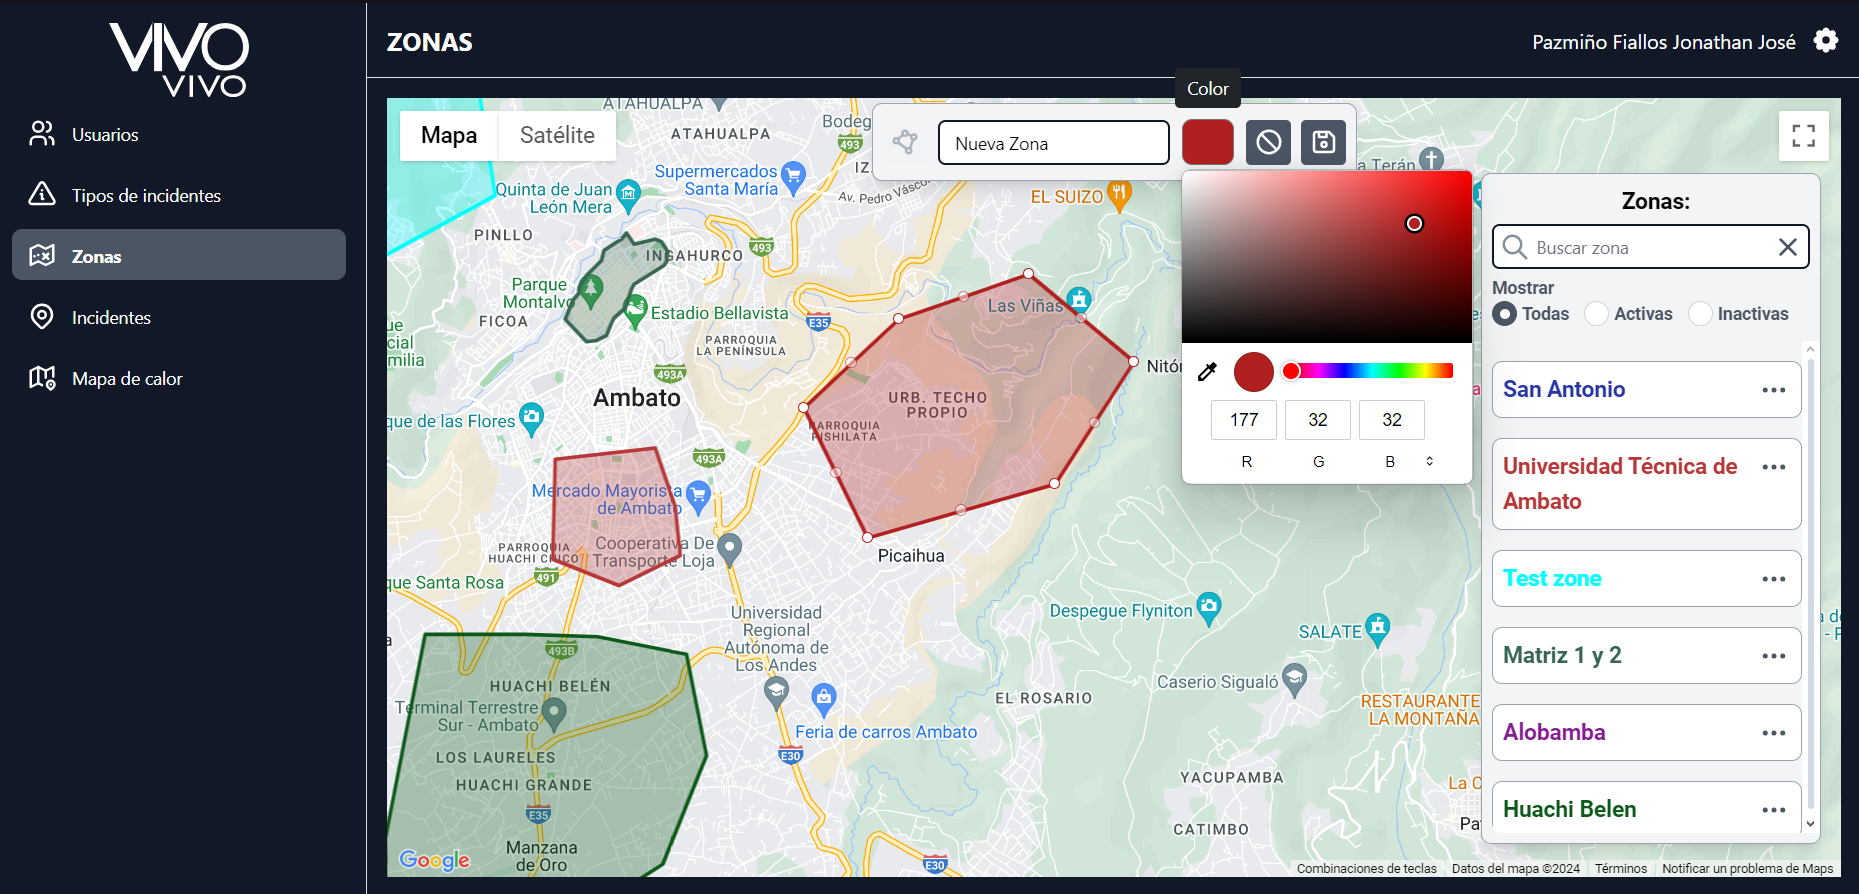
\includegraphics[width=0.8\textwidth]{chapters/III-resultados-y-discusion/resources/images/formulario-zona-vigilancia-web.png}
    \caption{Formulario para crear/editar zonas de vigilancia en el sistema web.}
    \label{fig:formulario-zona-vigilancia-web}
\end{figure}

\begin{figure}[H]
    \centering
    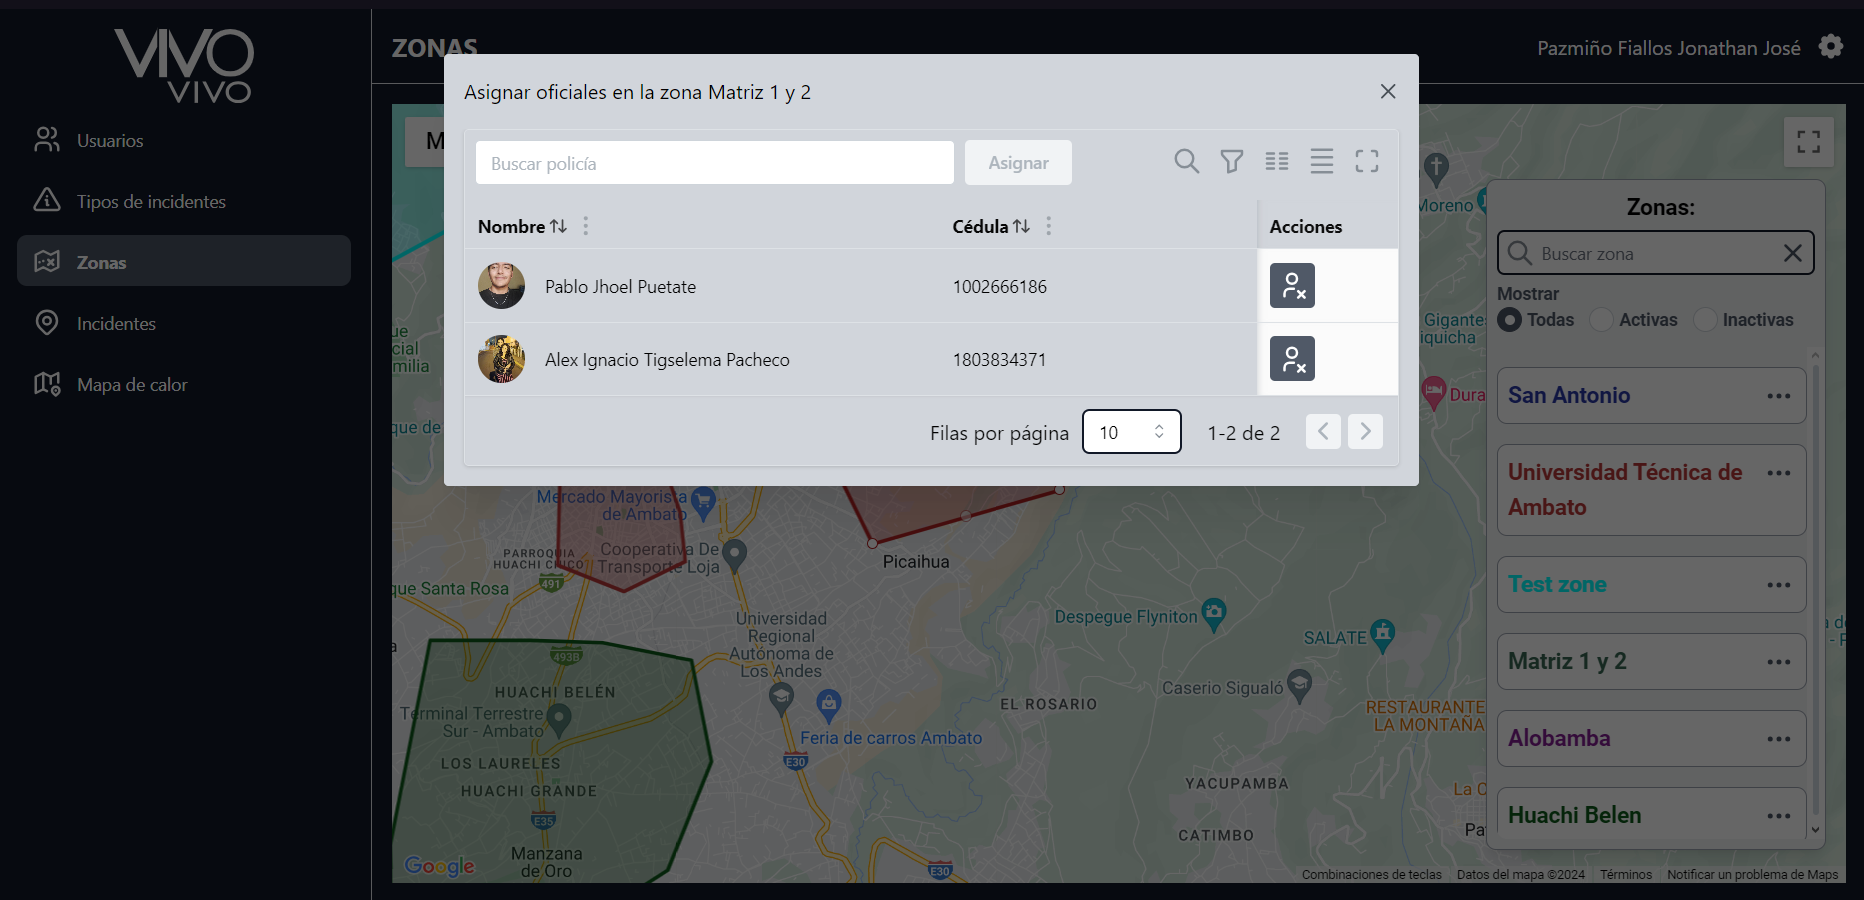
\includegraphics[width=0.8\textwidth]{chapters/III-resultados-y-discusion/resources/images/asignar-policias-zona-vigilancia-web.png}
    \caption{Asignar policías a zonas de vigilancia en el sistema web.}
    \label{fig:asignar-policias-zona-vigilancia-web}
\end{figure}

\paragraph{Gestión de incidentes}
La gestión de incidentes en el sistema web se realiza empleando un mapa interactivo, en el cual el usuario administrador puede visualizar
los incidentes reportados junto con la ubicación en tiempo real de la víctima, así como la ubicación de los policías en la zona de emergencia,
como se muestra en la Figura \ref{fig:mapa-incidentes-web}. El usuario administrador podrá visualizar el tipo de incidente y modificarlo en
caso de ser necesario. Además, podrá visualizar información de la víctima y de los policías asignados, como se puede observar en la Figura
\ref{fig:detalles-incidente-web}.

\begin{figure}[H]
    \centering
    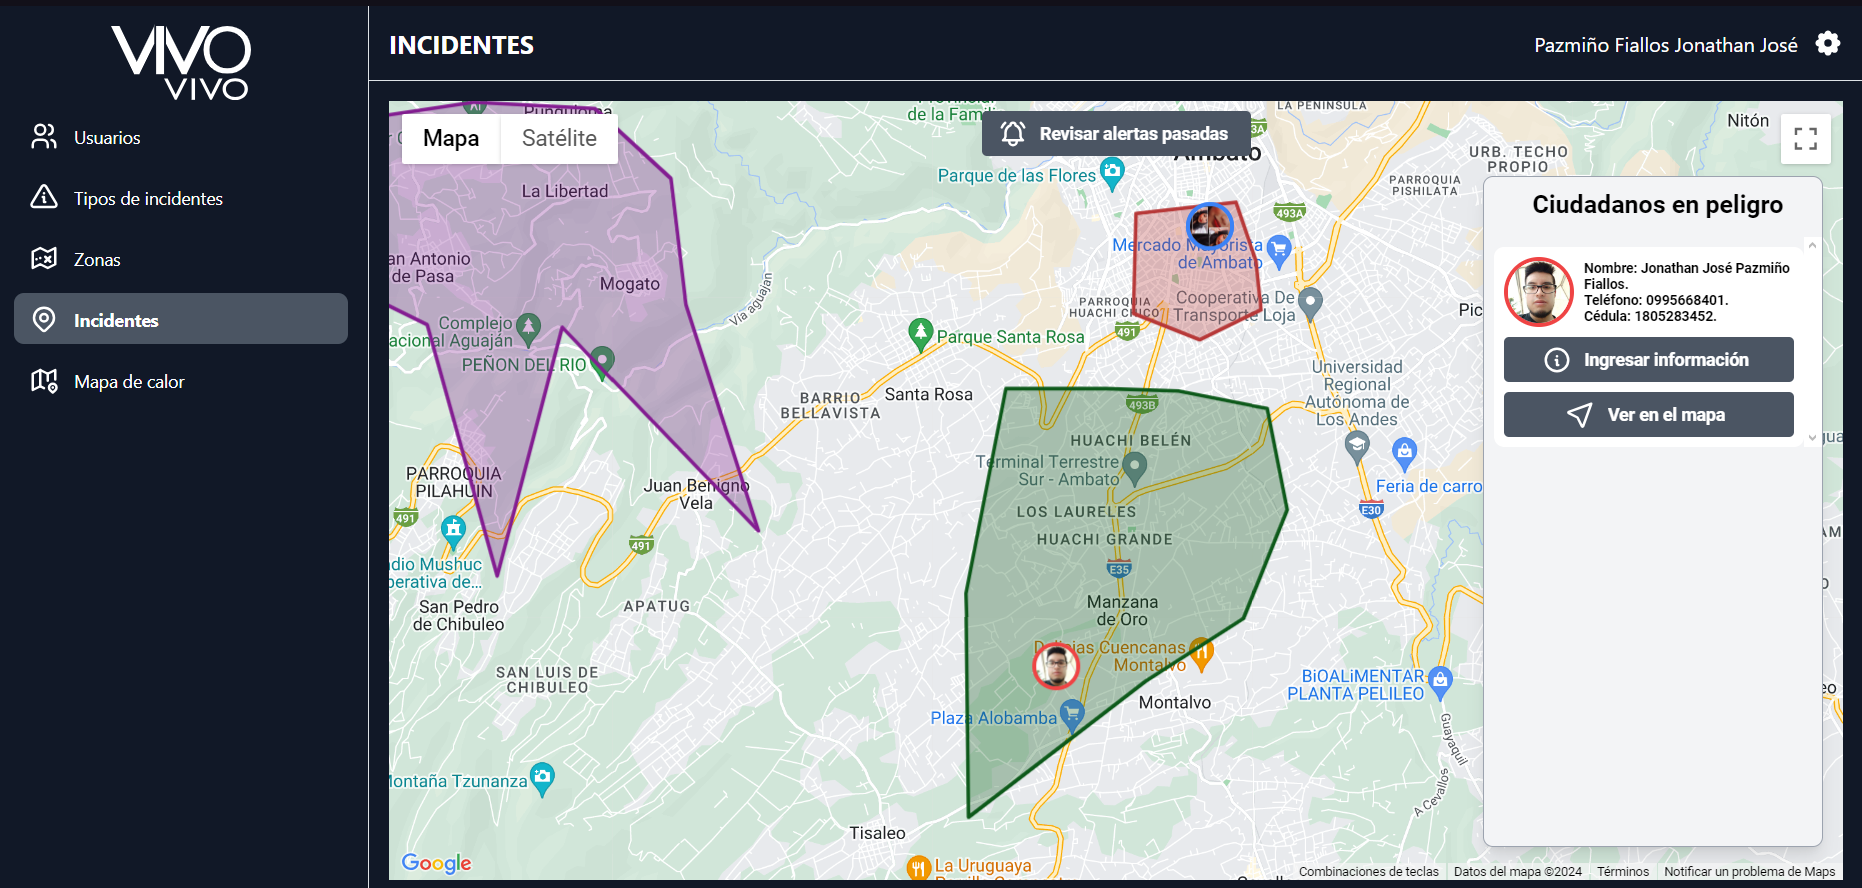
\includegraphics[width=0.8\textwidth]{chapters/III-resultados-y-discusion/resources/images/mapa-incidentes-web.png}
    \caption{Mapa de incidentes en el sistema web.}
    \label{fig:mapa-incidentes-web}
\end{figure}

\begin{figure}[H]
    \centering
    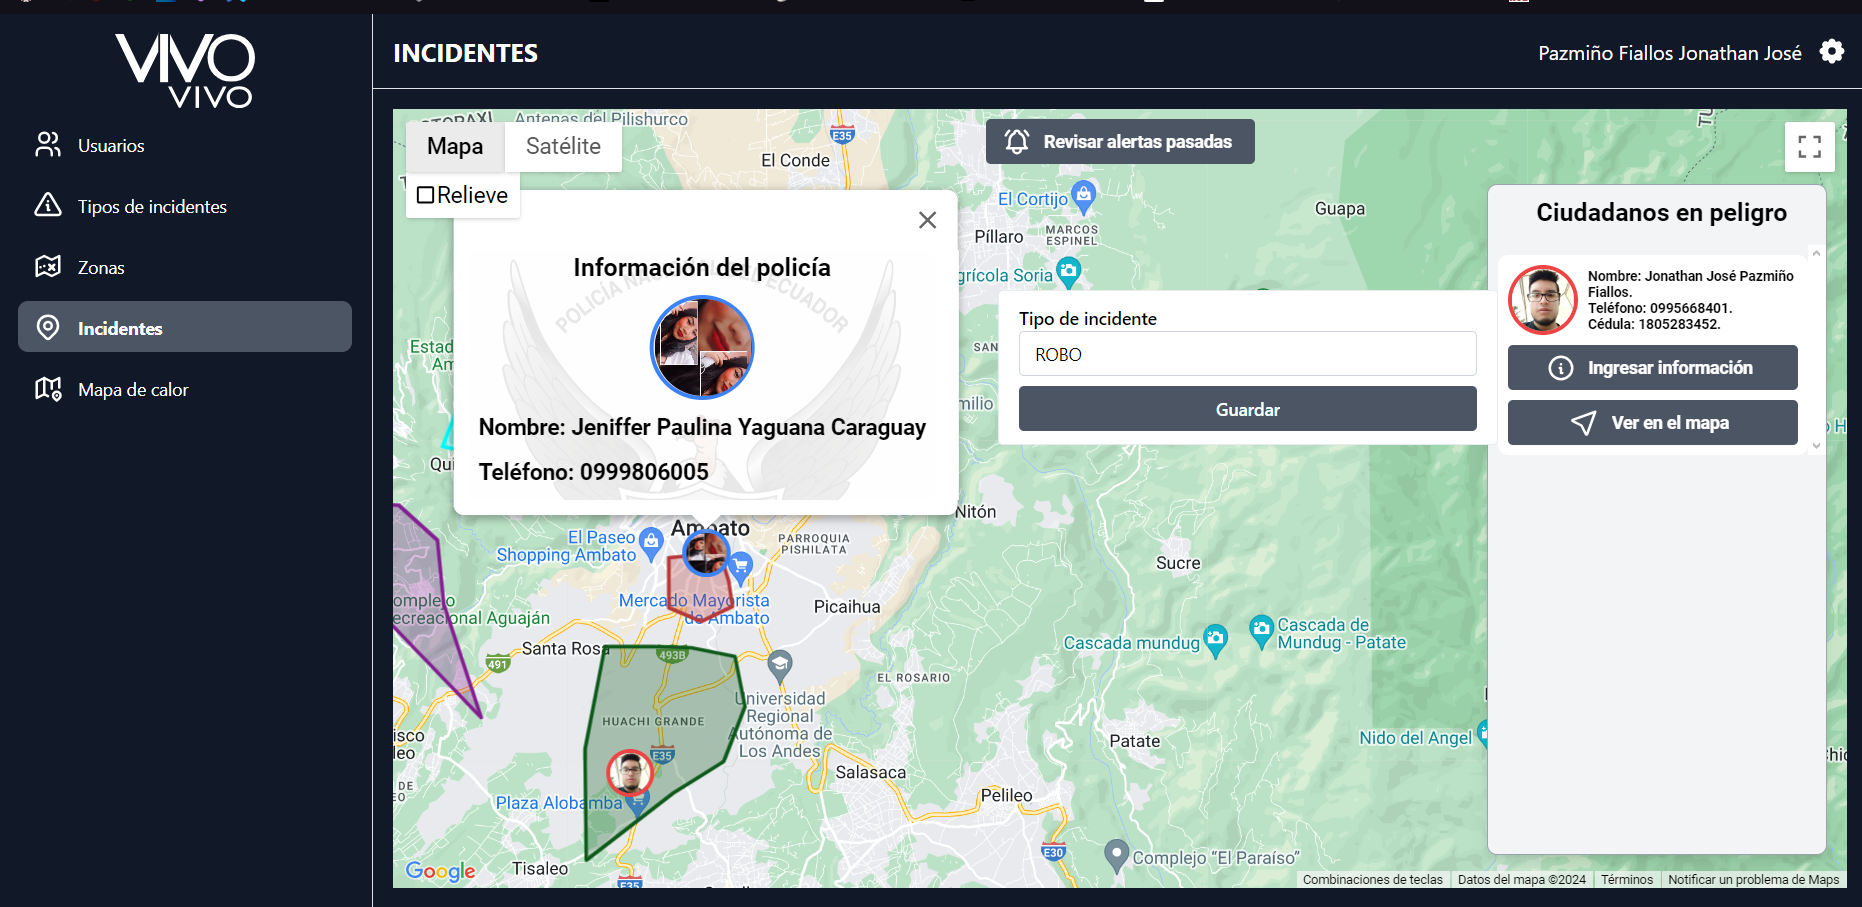
\includegraphics[width=0.8\textwidth]{chapters/III-resultados-y-discusion/resources/images/detalles-incidente-web.png}
    \caption{Detalles de incidente en el sistema web.}
    \label{fig:detalles-incidente-web}
\end{figure}

El usuario administrador podrá revisar las alertas de incidentes pasados mediante una tabla de entradas, en la cual se muestran los
campos de la información de los incidentes, como el tipo de incidente, la fecha y la ubicación, como se muestra en la Figura
\ref{fig:tabla-incidentes-web}.

\begin{figure}[H]
    \centering
    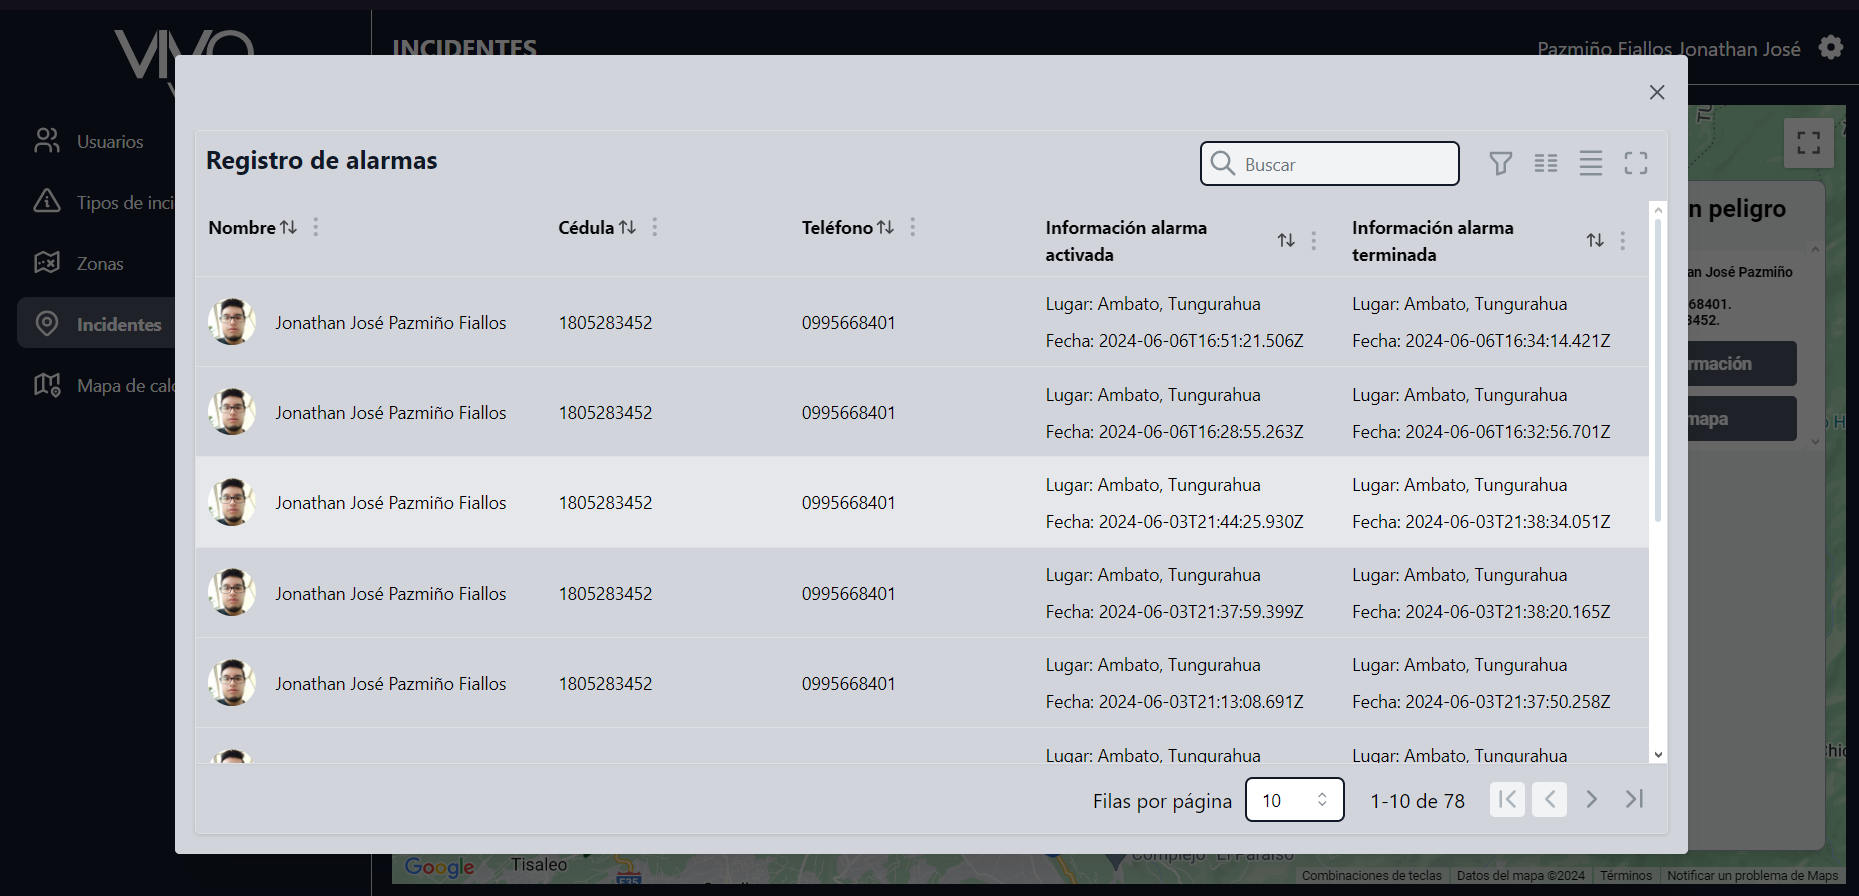
\includegraphics[width=0.8\textwidth]{chapters/III-resultados-y-discusion/resources/images/tabla-incidentes-web.png}
    \caption{Tabla de incidentes en el sistema web.}
    \label{fig:tabla-incidentes-web}
\end{figure}

\paragraph{Mapa de calor}
El mapa de calor en el sistema web permite al usuario administrador visualizar la densidad de incidentes reportados en un mapa
mediante un gradiente de colores, así como filtrar los incidentes por tipo y fecha, como se muestra en la Figura \ref{fig:mapa-de-calor-web}.

\begin{figure}[H]
    \centering
    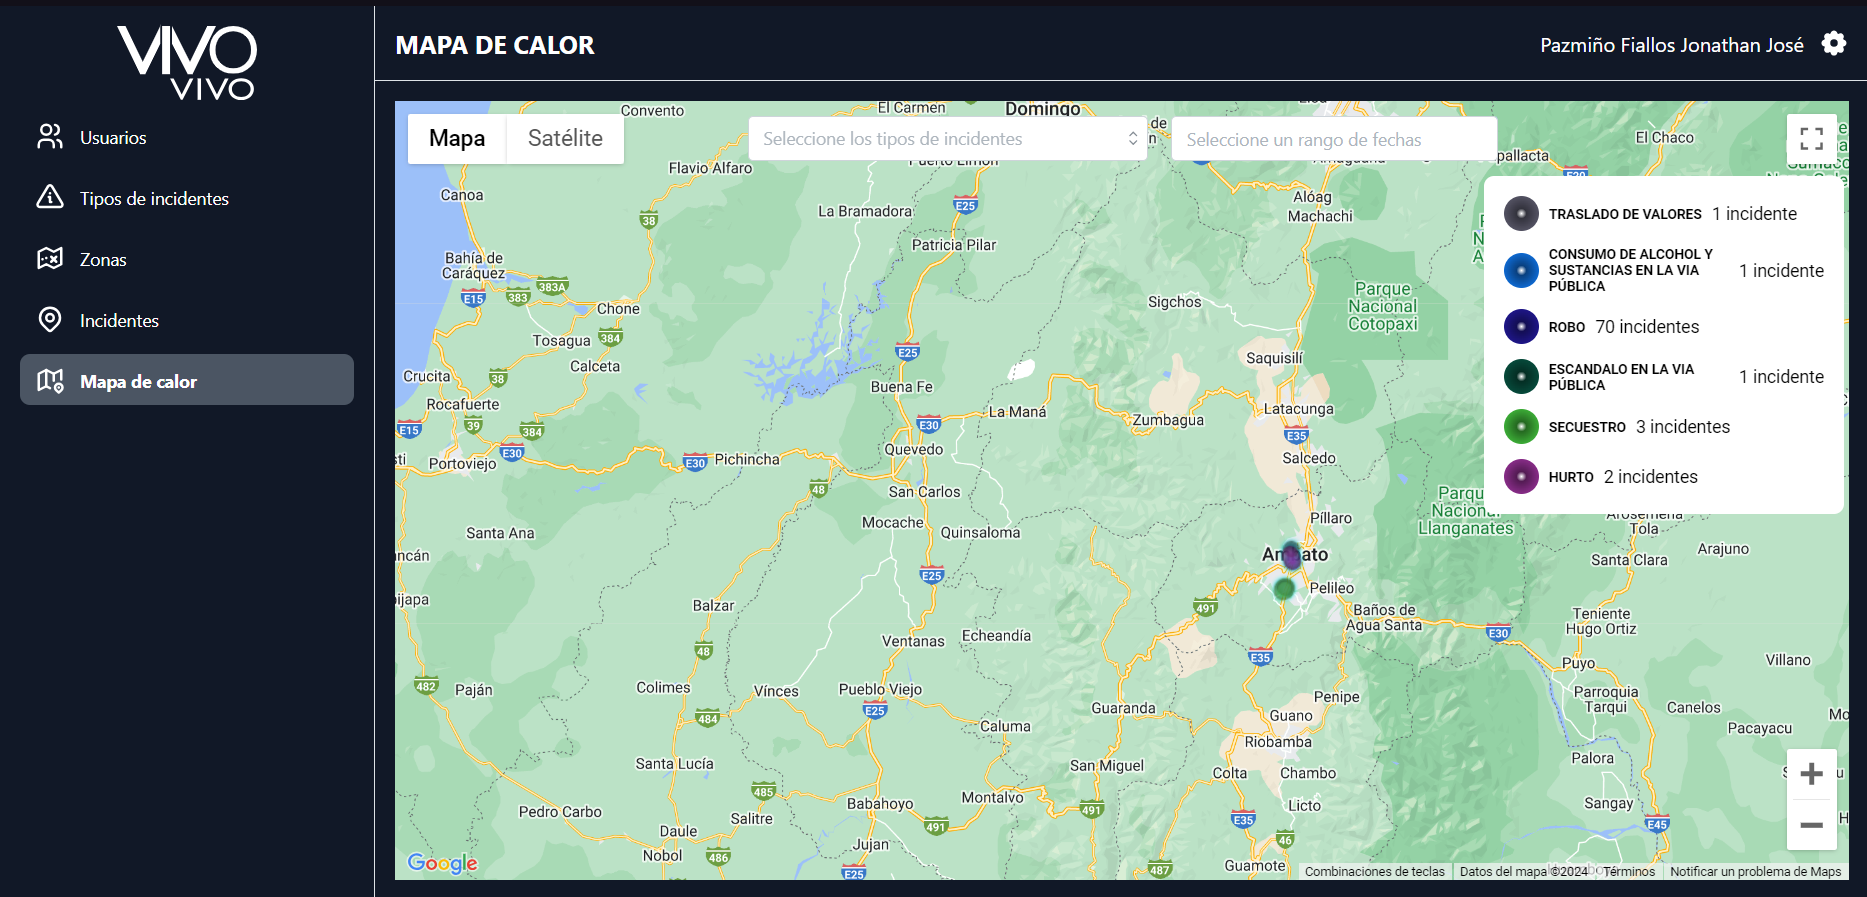
\includegraphics[width=0.8\textwidth]{chapters/III-resultados-y-discusion/resources/images/mapa-de-calor-web.png}
    \caption{Mapa de calor en el sistema web.}
    \label{fig:mapa-de-calor-web}
\end{figure}

\textbf{Aplicación móvil}
\bigbreak

\paragraph{Dependencias de la aplicación móvil}
Para crear el proyecto de Flutter se utilizó el comando \mintinline{text}{flutter create}, el cual crea una aplicación de Flutter con
una estructura de carpetas y archivos predefinida. Las dependencias utilizadas en la aplicación móvil se gestionaron mediante flutter pub
y el archivo de configuración pubspec.yaml. En el Anexo \ref{apendix:dependencias-movil} se muestra las dependencias utilizadas en la
aplicación móvil.

\paragraph{Configuración de variables de entorno de la aplicación móvil}
Para la configuración de las variables de entorno de la aplicación móvil se utilizó un archivo .env, el cual contiene las propiedades de
de la aplicación, como la URL de la API, el api key de Google Maps, el api key de OneSignal y la URL para obtener las imágenes
de Cloudinary. En el Anexo \ref{apendix:configuracion-env-movil} se muestra el archivo .env con las variables de entorno de la aplicación móvil.

\paragraph{Configuración de la aplicación}
En Flutter, la configuración global de la aplicación se realiza mediante Providers y ChangeNotifier, los cuales permiten compartir datos y
funcionalidades entre los widgets. En el Anexo \ref{apendix:configuracion-aplicacion-movil} se muestra la configuración para los
proveedores de sesión, sockets, localización y gestión de datos en la aplicación móvil.

\paragraph{Inicio de sesión}
El inicio de sesión en la aplicación móvil se realiza mediante un formulario en el cual el usuario ingresa su correo electrónico y
contraseña, como se muestra en la Figura \ref{fig:inicio-sesion-movil}. Estas credenciales son enviadas a la API mediante una solicitud
POST para autenticar al usuario y obtener un token JWT, el cual se almacena en el almacenamiento local del dispositivo para mantener
la sesión activa, en el Anexo \ref{apendix:guardar-token-movil} se muestra el código para guardar el token en el almacenamiento local del
dispositivo.

\begin{figure}[H]
    \centering
    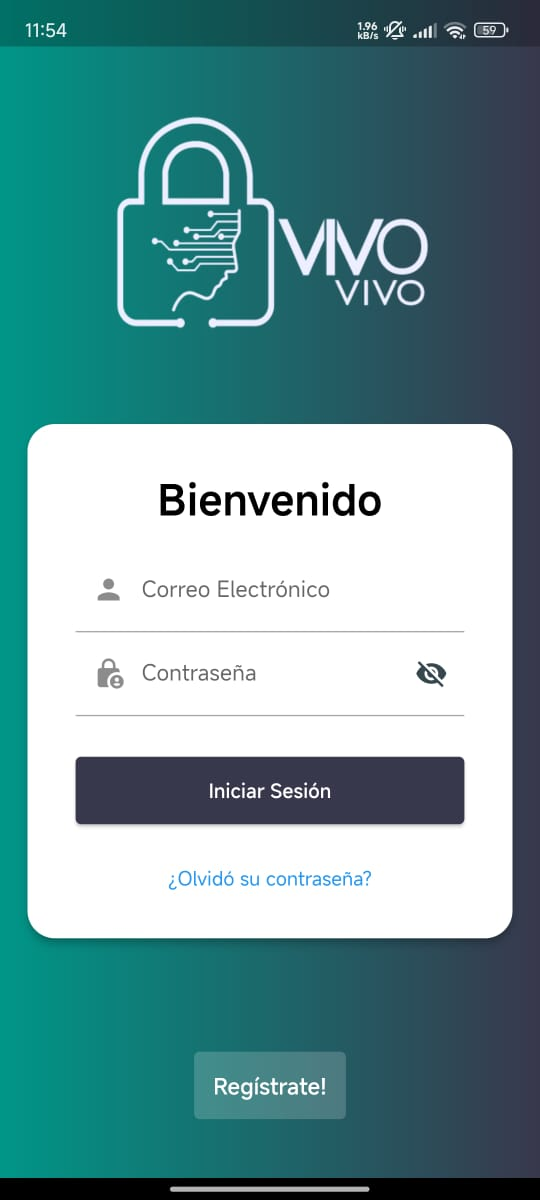
\includegraphics[width=0.3\textwidth]{chapters/III-resultados-y-discusion/resources/images/inicio-sesion-movil.png}
    \caption{Inicio de sesión en la aplicación móvil.}
    \label{fig:inicio-sesion-movil}
\end{figure}

\paragraph{Recuperar contraseña}
La recuperación de contraseña en la aplicación móvil se realiza mediante un formulario en el cual el usuario ingresa su correo electrónico,
como se muestra en la Figura \ref{fig:recuperar-contrasena-movil}. Una vez ingresado el correo electrónico, se envía una contraseña provisional
al correo electrónico del usuario con la cual podrá iniciar sesión y cambiar su contraseña, en la Figura \ref{fig:recuperar-contrasena-email}
se muestra el correo electrónico de recuperación de contraseña.

\begin{figure}[H]
    \centering
    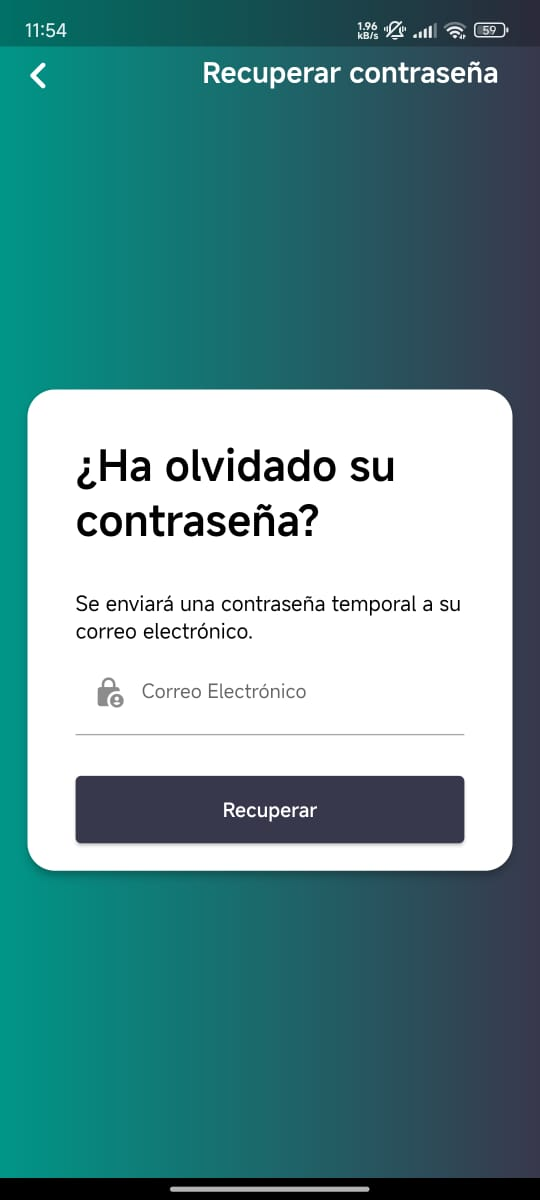
\includegraphics[width=0.3\textwidth]{chapters/III-resultados-y-discusion/resources/images/recuperar-contrasena-movil.png}
    \caption{Recuperar contraseña en la aplicación móvil.}
    \label{fig:recuperar-contrasena-movil}
\end{figure}

\begin{figure}[H]
    \centering
    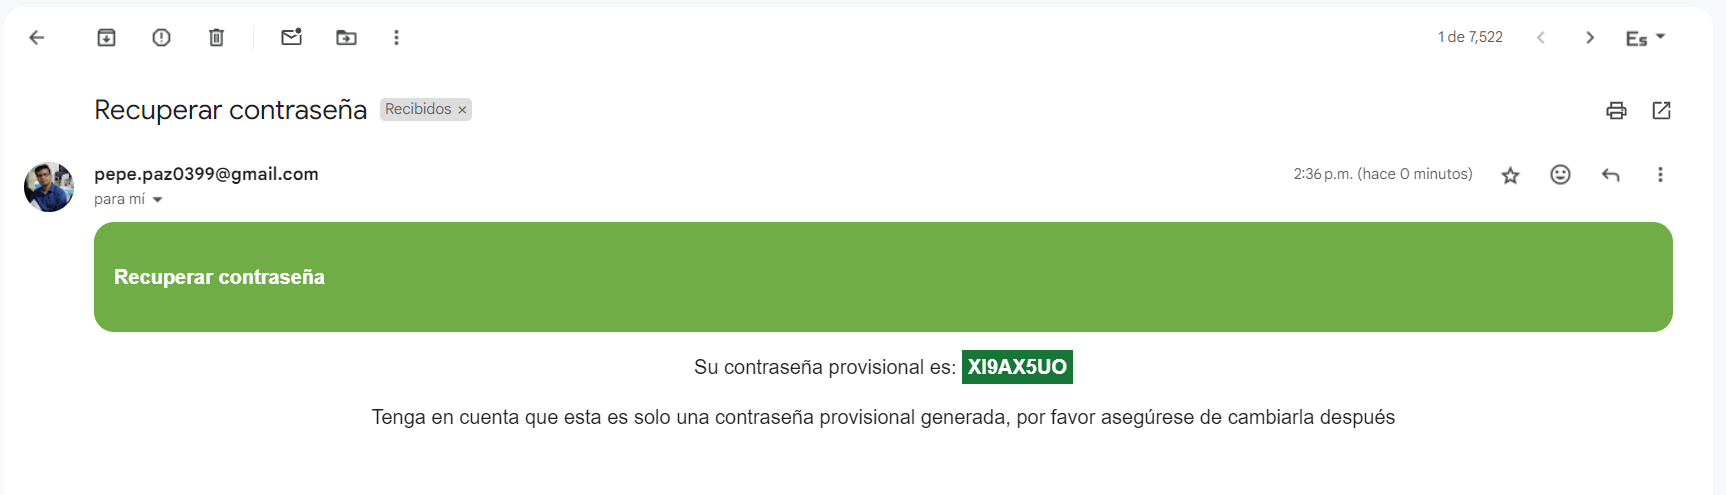
\includegraphics[width=1\textwidth]{chapters/III-resultados-y-discusion/resources/images/recuperar-contrasena-email.png}
    \caption{Correo electrónico de recuperación de contraseña.}
    \label{fig:recuperar-contrasena-email}
\end{figure}

\paragraph{Registro de usuario}
El registro de usuario en la aplicación móvil se realiza mediante un formulario en el cual el usuario ingresa su información personal,
como nombres, apellidos, correo electrónico, contraseña, género, etnia, entre otros, como se muestra en las Figuras \ref{fig:registro-usuario-movil-1}
y \ref{fig:registro-usuario-movil-2}. Para ingresar la dirección del usuario, se utilizó un campo de búsqueda de direcciones que permite
al usuario buscar su dirección en un mapa interactivo y seleccionarla, como se muestra en la Figura \ref{fig:registro-usuario-movil-3}.

\begin{figure}[H]
    \centering
    \includegraphics[width=0.3\textwidth]{chapters/III-resultados-y-discusion/resources/images/registro-usuario-movil-1.png}
    \caption{Registro de usuario en la aplicación móvil (Parte 1).}
    \label{fig:registro-usuario-movil-1}
\end{figure}

\begin{figure}[H]
    \centering
    \includegraphics[width=0.3\textwidth]{chapters/III-resultados-y-discusion/resources/images/registro-usuario-movil-2.png}
    \caption{Registro de usuario en la aplicación móvil (Parte 2).}
    \label{fig:registro-usuario-movil-2}
\end{figure}

\begin{figure}[H]
    \centering
    \includegraphics[width=0.3\textwidth]{chapters/III-resultados-y-discusion/resources/images/registro-usuario-movil-3.png}
    \caption{Registro de usuario en la aplicación móvil (Parte 3).}
    \label{fig:registro-usuario-movil-3}
\end{figure}

\paragraph{Pantalla principal}
La pantalla principal de la aplicación móvil muestra el botón de pánico en la parte central de la pantalla, el cual permite al usuario
enviar una alerta de emergencia a los miembros de su grupo familiar y a los policías en la zona de emergencia presionando el botón
durante 3 segundos, también el usuario puede seleccionar el tipo de incidente mediante un check, como se muestra en la Figura
\ref{fig:pantalla-principal-movil}.

\begin{figure}[H]
    \centering
    \includegraphics[width=0.3\textwidth]{chapters/III-resultados-y-discusion/resources/images/pantalla-principal-movil.png}
    \caption{Pantalla principal de la aplicación móvil.}
    \label{fig:pantalla-principal-movil}
\end{figure}

\paragraph{Menú de usuario}
El menú de usuario en la aplicación móvil permite al usuario acceder a las opciones tales como cambiar contraseña, cerrar sesión y
gestionar el grupo familiar, como se muestra en la Figura \ref{fig:menu-usuario-movil}.

\begin{figure}[H]
    \centering
    \includegraphics[width=0.3\textwidth]{chapters/III-resultados-y-discusion/resources/images/menu-usuario-movil.png}
    \caption{Menú de usuario en la aplicación móvil.}
    \label{fig:menu-usuario-movil}
\end{figure}

\paragraph{Gestión de grupo familiar}
La gestión del grupo familiar en la aplicación móvil se realiza mediante una lista en la cual el usuario podrá visualizar a
los miembros de su grupo familiar, como se muestra en la Figura \ref{fig:grupo-familiar-movil}. El usuario podrá agregar
miembros a su grupo familiar mediante un formulario en el cual ingresará la cédula de identidad del usuario que desee
agregar, como se muestra en la Figura \ref{fig:agregar-miembro-movil}.

\begin{figure}[H]
    \centering
    \includegraphics[width=0.3\textwidth]{chapters/III-resultados-y-discusion/resources/images/grupo-familiar-movil.png}
    \caption{Gestión de grupo familiar en la aplicación móvil.}
    \label{fig:grupo-familiar-movil}
\end{figure}

\begin{figure}[H]
    \centering
    \includegraphics[width=0.3\textwidth]{chapters/III-resultados-y-discusion/resources/images/agregar-miembro-movil.png}
    \caption{Agregar miembro al grupo familiar en la aplicación móvil.}
    \label{fig:agregar-miembro-movil}
\end{figure}

\paragraph{Cambiar contraseña}
La opción de cambiar contraseña en la aplicación móvil permite al usuario modificar su contraseña ingresando la contraseña actual,
la nueva contraseña y la confirmación de la nueva contraseña, como se muestra en la Figura \ref{fig:cambiar-contrasena-movil}.

\begin{figure}[H]
    \centering
    \includegraphics[width=0.3\textwidth]{chapters/III-resultados-y-discusion/resources/images/cambiar-contrasena-movil.png}
    \caption{Cambiar contraseña en la aplicación móvil.}
    \label{fig:cambiar-contrasena-movil}
\end{figure}

\paragraph{Alertas recibidas}
Las alertas recibidas en la aplicación móvil se visualizan mediante una lista en la cual se muestra el estado de cada miembro del
grupo familiar. Cuando un miembro del grupo familiar envía una alerta de emergencia, se muestra una notificación en el dispositivo
del usuario, como se puede observar en la Figura \ref{fig:notificacion-recibida-movil} y el estado del miembro cambia a "En peligro", como se
puede observar en la Figura \ref{fig:alerta-recibida-movil}. El usuario podrá visualizar la ubicación en tiempo real del miembro en
peligro seleccionando el botón "Seguir ubicación", lo cual mostrará la en un mapa la ubicación del miembro en peligro y la ubicación
del usuario, como se muestra en la Figura \ref{fig:seguir-ubicacion-movil}.

\begin{figure}[H]
    \centering
    \includegraphics[width=0.3\textwidth]{chapters/III-resultados-y-discusion/resources/images/notificacion-recibida-movil.png}
    \caption{Notificación de alerta recibida en la aplicación móvil.}
    \label{fig:notificacion-recibida-movil}
\end{figure}

\begin{figure}[H]
    \centering
    \includegraphics[width=0.3\textwidth]{chapters/III-resultados-y-discusion/resources/images/alerta-recibida-movil.png}
    \caption{Alerta recibida en la aplicación móvil.}
    \label{fig:alerta-recibida-movil}
\end{figure}

\begin{figure}[H]
    \centering
    \includegraphics[width=0.3\textwidth]{chapters/III-resultados-y-discusion/resources/images/seguir-ubicacion-movil.png}
    \caption{Seguir ubicación en la aplicación móvil.}
    \label{fig:seguir-ubicacion-movil}
\end{figure}

\textbf{Modelo analítico de BI}
\bigbreak

Para el diseño del modelo analítico de BI se utilizó la metodología Hefesto, ya que esta facilita la construcción de un
Data Warehouse y aporta información útil para mejorar el rendimiento \cite{darioDATAWAREHOUSINGMarco}.

% \paragraph{Carta de diseño para el modelo dimensional}

La carta de diseño para el modelo dimensional se utiliza para describir el proceso de diseño de un modelo dimensional
siguiendo los pasos de la metodología Hefesto. Estos pasos incluyen la selección del proceso de negocio, la declaración
del grano, la identificación de las dimensiones y sus atributos, la identificación de las tablas de hechos y sus métricas,
y el diseño del esquema dimensional. A continuación, se presenta cada uno de estos pasos.

\begin{itemize}
    \item Seleccionar el proceso de negocio:
          \begin{itemize}
              \item Identificar las pregustas del negocio.
              \item Identificar indicadores y perspectivas.
              \item Diseñar el modelo conceptual.
          \end{itemize}
    \item Declarar el grano.
    \item Identificar las dimensiones y sus atributos.
    \item Identificar las tablas de hechos y sus métricas.
    \item Diseñar el esquema dimensional
\end{itemize}

\paragraph{Seleccionar el proceso de negocio}

\paragraph{Preguntas del negocio}

El objetivo principal del sistema de reportería de incidentes delictivos es recolectar y analizar información
sobre los incidentes delictivos reportados a través de un sistema de alarma, así como detalles de los usuarios
y datos geográficos relevantes para apoyar la toma de decisiones de las autoridades policiales.

\paragraph{Identificar indicadores y perspectivas}

\begin{itemize}
    \item Determinar el número de incidentes por tipo de incidente y zona de vigilancia.
    \item Analizar la distribución de incidentes por género, discapacidad, etnia y edad de los usuarios.
    \item Identificar las zonas con mayor número de incidentes para optimizar la vigilancia policial.
\end{itemize}

\begin{longtable}{|p{5cm}|p{5cm}|}
    \caption{Indicadores y perspectivas en base las pregustas de negocio} \label{tab:indicadores-perspectivas} \\

    \hline \multicolumn{1}{|c|}{\textbf{Indicadores}} & \multicolumn{1}{|c|}{\textbf{Perspectivas}}            \\ \hline
    \endfirsthead

    \multicolumn{2}{c}%
    {{\normalfont \tablename\ \thetable{} -- continuación de la página anterior}}                              \\
    \hline \multicolumn{1}{|c|}{\textbf{Indicadores}} & \multicolumn{1}{|c|}{\textbf{Perspectivas}}            \\ \hline
    \endhead

    \hline \multicolumn{2}{|r|}{{Continua en la siguiente página}}                                             \\ \hline
    \endfoot

    \hline \hline
    \endlastfoot
    Número de incidentes                              & Tipo de Alarma                                         \\\hline
    Número de incidentes                              & Tipo de Incidente                                      \\\hline
    Número de incidentes                              & Zona de Vigilancia                                     \\\hline
    Número de incidentes                              & Género, Discapacidad, Etnia, Estado Civil              \\
\end{longtable}

En base a los indicadores y perspectivas identificados, se estableció como KPI principal el número de incidentes
delictivos reportados, ya que este indicador permite medir la frecuencia de los delitos reportados en una determinada
área o periodo de tiempo.

\paragraph{Declarar el grano}

El grano del modelo dimensional es un único incidente delictivo reportado. Esto implica que cada registro en la
tabla de hechos representa un incidente específico.

\paragraph{Identificar las dimensiones y sus atributos}

En las Tablas \ref{tab:dimension-tiempo}, \ref{tab:dimension-usuarios}, \ref{tab:dimension-tipo-de-alarma},
\ref{tab:dimension-tipo-de-incidente} y \ref{tab:dimension-zona-de-vigilancia} se presentan las dimensiones y
sus atributos identificados para el modelo dimensional.

\begin{longtable}{|p{6cm}|p{6cm}|}
    \caption{Dimensión de tiempo con sus atributos} \label{tab:dimension-tiempo}             \\

    \hline \multicolumn{1}{|c|}{\textbf{Campo}} & \multicolumn{1}{|c|}{\textbf{Descripción}} \\ \hline
    \endfirsthead

    \multicolumn{2}{c}%
    {{\normalfont \tablename\ \thetable{} -- continuación de la página anterior}}            \\
    \hline \multicolumn{1}{|c|}{\textbf{Campo}} & \multicolumn{1}{|c|}{\textbf{Descripción}} \\ \hline
    \endhead

    \hline \multicolumn{2}{|r|}{{Continua en la siguiente página}}                           \\ \hline
    \endfoot

    \hline \hline
    \endlastfoot
    fechaID                                     & Identificador único para cada fecha        \\\hline
    fecha                                       & Fecha completa del incidente (YYYY-MM-DD)  \\\hline
    anio                                        & Año en que ocurrió el incidente            \\\hline
    mes                                         & Mes en que ocurrió el incidente            \\\hline
    día                                         & Día en que ocurrió el incidente            \\\hline
    trimestre                                   & Trimestre en que ocurrió el incidente      \\\hline
    semestre                                    & Semestre en que ocurrió el incidente       \\\hline
    hora                                        & Hora en que ocurrió el incidente           \\
\end{longtable}

\begin{longtable}{|p{6cm}|p{6cm}|}
    \caption{Dimensión de usuarios con sus atributos} \label{tab:dimension-usuarios}         \\

    \hline \multicolumn{1}{|c|}{\textbf{Campo}} & \multicolumn{1}{|c|}{\textbf{Descripción}} \\ \hline
    \endfirsthead

    \multicolumn{2}{c}%
    {{\normalfont \tablename\ \thetable{} -- continuación de la página anterior}}            \\
    \hline \multicolumn{1}{|c|}{\textbf{Campo}} & \multicolumn{1}{|c|}{\textbf{Descripción}} \\ \hline
    \endhead

    \hline \multicolumn{2}{|r|}{{Continua en la siguiente página}}                           \\ \hline
    \endfoot

    \hline \hline
    \endlastfoot
    usuarioID                                   & Identificador único del usuario            \\\hline
    género                                      & Género del usuario                         \\\hline
    discapacidad                                & Estado de discapacidad del usuario         \\\hline
    etnia                                       & Etnia del usuario                          \\\hline
    estadoCivil                                 & Estado civil del usuario                   \\\hline
    edad                                        & Edad del usuario                           \\
\end{longtable}

\begin{longtable}{|p{6cm}|p{6cm}|}
    \caption{Dimensión de tipo de alarma con sus atributos} \label{tab:dimension-tipo-de-alarma} \\

    \hline \multicolumn{1}{|c|}{\textbf{Campo}} & \multicolumn{1}{|c|}{\textbf{Descripción}}     \\ \hline
    \endfirsthead

    \multicolumn{2}{c}%
    {{\normalfont \tablename\ \thetable{} -- continuación de la página anterior}}                \\
    \hline \multicolumn{1}{|c|}{\textbf{Campo}} & \multicolumn{1}{|c|}{\textbf{Descripción}}     \\ \hline
    \endhead

    \hline \multicolumn{2}{|r|}{{Continua en la siguiente página}}                               \\ \hline
    \endfoot

    \hline \hline
    \endlastfoot
    tipoAlarmaID                                & Identificador único del tipo de alarma         \\\hline
    nombreTipoAlarma                            & Nombre del tipo de alarma                      \\
\end{longtable}

\begin{longtable}{|p{6cm}|p{6cm}|}
    \caption{Dimensión de tipo de incidente con sus atributos} \label{tab:dimension-tipo-de-incidente} \\

    \hline \multicolumn{1}{|c|}{\textbf{Campo}} & \multicolumn{1}{|c|}{\textbf{Descripción}}           \\ \hline
    \endfirsthead

    \multicolumn{2}{c}%
    {{\normalfont \tablename\ \thetable{} -- continuación de la página anterior}}                      \\
    \hline \multicolumn{1}{|c|}{\textbf{Campo}} & \multicolumn{1}{|c|}{\textbf{Descripción}}           \\ \hline
    \endhead

    \hline \multicolumn{2}{|r|}{{Continua en la siguiente página}}                                     \\ \hline
    \endfoot

    \hline \hline
    \endlastfoot
    tipoIncidenteID                             & Identificador único del tipo de incidente            \\\hline
    nombreTipoIncidente                         & Nombre del tipo de incidente                         \\
\end{longtable}

\begin{longtable}{|p{6cm}|p{6cm}|}
    \caption{Dimensión de zonas de vigilancia con sus atributos} \label{tab:dimension-zonas-vigilancia} \\

    \hline \multicolumn{1}{|c|}{\textbf{Campo}} & \multicolumn{1}{|c|}{\textbf{Descripción}}            \\ \hline
    \endfirsthead

    \multicolumn{2}{c}%
    {{\normalfont \tablename\ \thetable{} -- continuación de la página anterior}}                       \\
    \hline \multicolumn{1}{|c|}{\textbf{Campo}} & \multicolumn{1}{|c|}{\textbf{Descripción}}            \\ \hline
    \endhead

    \hline \multicolumn{2}{|r|}{{Continua en la siguiente página}}                                      \\ \hline
    \endfoot

    \hline \hline
    \endlastfoot
    zonaVigilanciaID                            & Identificador único de la zona de vigilancia          \\\hline
    polígono                                    & Representación geográfica de la zona de vigilancia    \\\hline
    nombreZonaVigilancia                        & Nombre de la zona de vigilancia                       \\
\end{longtable}

\begin{longtable}{|p{6cm}|p{6cm}|}
    \caption{Dimensión de ubicación con sus atributos} \label{tab:dimension-zonas-vigilancia} \\

    \hline \multicolumn{1}{|c|}{\textbf{Campo}} & \multicolumn{1}{|c|}{\textbf{Descripción}}  \\ \hline
    \endfirsthead

    \multicolumn{2}{c}%
    {{\normalfont \tablename\ \thetable{} -- continuación de la página anterior}}             \\
    \hline \multicolumn{1}{|c|}{\textbf{Campo}} & \multicolumn{1}{|c|}{\textbf{Descripción}}  \\ \hline
    \endhead

    \hline \multicolumn{2}{|r|}{{Continua en la siguiente página}}                            \\ \hline
    \endfoot

    \hline \hline
    \endlastfoot
    ubicacionID                                 & Identificador único de la ubicación         \\\hline
    canton                                      & Cantón del lugar del incidente              \\\hline
    ciudad                                      & Ciudad del lugar del incidente              \\
\end{longtable}

\paragraph{Identificar las tablas de hechos y sus métricas}

En la Tabla \ref{tab:hechos-incidentes-delictivos} se presentan los hechos de incidentes delictivos y sus atributos.

\begin{longtable}{|p{6cm}|p{6cm}|}
    \caption{Hechos de incidentes delictivos con sus atributos} \label{tab:hechos-incidentes-delictivos}     \\

    \hline \multicolumn{1}{|c|}{\textbf{Campo}} & \multicolumn{1}{|c|}{\textbf{Descripción}}                 \\ \hline
    \endfirsthead

    \multicolumn{2}{c}%
    {{\normalfont \tablename\ \thetable{} -- continuación de la página anterior}}                            \\
    \hline \multicolumn{1}{|c|}{\textbf{Campo}} & \multicolumn{1}{|c|}{\textbf{Descripción}}                 \\ \hline
    \endhead

    \hline \multicolumn{2}{|r|}{{Continua en la siguiente página}}                                           \\ \hline
    \endfoot

    \hline \hline
    \endlastfoot
    incidenteID                                 & Clave primaria de la tabla de hechos incidentes delictivos \\\hline
    fechaID                                     & Clave foránea a la dimensión de tiempo                     \\\hline
    usuarioID                                   & Clave foránea a la dimensión de usuarios                   \\\hline
    tipoAlarmaID                                & Clave foránea a la dimensión de tipo de alarma             \\\hline
    tipoIncidenteID                             & Clave foránea a la dimensión de tipo de incidente          \\\hline
    zonaVigilanciaID                            & Clave foránea a la dimensión de zonas de vigilancia        \\\hline
    ubicacionID                                 & Clave foránea a la dimensión de ubicación geográfica       \\\hline
    numeroIncidentes                            & Número de incidentes reportados                            \\\hline
\end{longtable}

\paragraph{Esquema dimensional}

En la Figura \ref{fig:esquema-modelo-dimensional} se muestra el esquema del modelo dimensional propuesto para el sistema de reportería de incidentes delictivos.

\begin{figure}[H]
    \centering
    \includegraphics[width=1\textwidth]{chapters/III-resultados-y-discusion/resources/images/esquema-modelo-dimensional.png}
    \caption{Esquema del modelo dimensional para el sistema de reportería de incidentes delictivos}
    \label{fig:esquema-modelo-dimensional}
\end{figure}

\paragraph{Proceso ETL}

Una vez definido el modelo dimensional, se procedió a diseñar el proceso de extracción, transformación y carga (ETL) de los datos.
Para ello, se utilizó la herramienta de ETL de visual studio, la cual permite extraer datos de diferentes fuentes, transformarlos
y cargarlos en el modelo dimensional. En la Figura \ref{fig:etl-bi} se muestra el diseño del proceso ETL para el modelo dimensional.

\begin{figure}[H]
    \centering
    \includegraphics[width=0.8\textwidth]{chapters/III-resultados-y-discusion/resources/images/etl-bi.png}
    \caption{Diseño del proceso ETL para el modelo dimensional.}
    \label{fig:etl-bi}
\end{figure}

El proceso ETL inicia con la limpieza de las tablas que componen el modelo dimensional. Esto se realiza mediante la ejecución de un
script SQL que elimina los registros de las tablas de hechos y dimensiones, como se puede observar en la Figura\ref{fig:limpieza-bi}.
Una vez limpias las tablas, se procede a extraer los datos de las fuentes de datos. En este caso, se utilizó un origen de datos de
ADO.NET para extraer los datos desde PostgreSQL. Además, se utilizó el componente de Data Conversion para convertir los datos a un
formato compatible con el destino en una base de datos de SQL Server. Finalmente, se cargan los datos mediante el componente de OLE
DB Destination, como se puede observar en la Figura \ref{fig:extraccion-bi}.

\begin{figure}[H]
    \centering
    \includegraphics[width=0.8\textwidth]{chapters/III-resultados-y-discusion/resources/images/limpieza-bi.png}
    \caption{Limpieza de las tablas del modelo dimensional.}
    \label{fig:limpieza-bi}
\end{figure}

\begin{figure}[H]
    \centering
    \includegraphics[width=0.8\textwidth]{chapters/III-resultados-y-discusion/resources/images/extraccion-bi.png}
    \caption{Extracción de datos para el modelo dimensional.}
    \label{fig:extraccion-bi}
\end{figure}

Al ejecutar el proceso ETL, se comienza con la extracción siguiendo el flujo de datos definido en el proceso ETL. En caso de no
existir ningún error, el sistema mostrará un mensaje de éxito, como se puede observar en la Figura \ref{fig:exito-bi}.

\begin{figure}[H]
    \centering
    \includegraphics[width=0.8\textwidth]{chapters/III-resultados-y-discusion/resources/images/exito-bi.png}
    \caption{Mensaje de éxito al ejecutar el proceso ETL.}
    \label{fig:exito-bi}
\end{figure}

\pagebreak{Cubo OLAP}
Para la construcción del cubo OLAP se empleó Visual Studio Community 2022, creando un proyecto de Analysis Services. En este
proyecto, se definió la conexión a la base de datos de SQL Server, como se muestra en la Figura \ref{fig:conexion-olap},
se creó un origen de datos, como se puede observar en la Figura \ref{fig:origen-datos-olap}, y se diseñó el cubo OLAP, como se
puede visualizar en la Figura \ref{fig:cubo-olap}.

\begin{figure}[H]
    \centering
    \includegraphics[width=0.8\textwidth]{chapters/III-resultados-y-discusion/resources/images/conexion-olap.png}
    \caption{Conexión a la base de datos de SQL Server en el proyecto de Analysis Services.}
    \label{fig:conexion-olap}
\end{figure}

\begin{figure}[H]
    \centering
    \includegraphics[width=0.8\textwidth]{chapters/III-resultados-y-discusion/resources/images/origen-datos-olap.png}
    \caption{Origen de datos en el proyecto de Analysis Services.}
    \label{fig:origen-datos-olap}
\end{figure}

\begin{figure}[H]
    \centering
    \includegraphics[width=0.8\textwidth]{chapters/III-resultados-y-discusion/resources/images/cubo-olap.png}
    \caption{Diseño del cubo OLAP en el proyecto de Analysis Services.}
    \label{fig:cubo-olap}
\end{figure}

En el origen de datos se definieron campos creados mediante cálculos con nombre que permiten agregar medidas e información
adicional al cubo OLAP, como se puede observar en la Figura \ref{fig:campos-origen-datos-olap}.

\begin{figure}[H]
    \centering
    \includegraphics[width=0.8\textwidth]{chapters/III-resultados-y-discusion/resources/images/campos-origen-datos-olap.png}
    \caption{Campos en el origen de datos del proyecto de Analysis Services.}
    \label{fig:campos-origen-datos-olap}
\end{figure}

En la dimension de tiempo se definieron jerarquías de tiempo que permiten visualizar los datos de forma secuencial en años, meses,
días y horas, como se puede observar en la Figura \ref{fig:dimension-tiempo-olap}.

\begin{figure}[H]
    \centering
    \includegraphics[width=0.8\textwidth]{chapters/III-resultados-y-discusion/resources/images/dimension-tiempo-olap.png}
    \caption{Jerarquías de tiempo en la dimensión de tiempo del proyecto de Analysis Services.}
    \label{fig:dimension-tiempo-olap}
\end{figure}

Una vez definido el cubo OLAP, se procedió a procesarlo para generar las medidas e indicadores definidos en el modelo dimensional, terminado
el proceso de procesamiento se muestra un mensaje de éxito y se muestra el examinador de cubos en el cual se pueden realizar consultas a los
datos del cubo OLAP, como se puede observar en la Figura \ref{fig:exito-olap}.

\begin{figure}[H]
    \centering
    \includegraphics[width=0.8\textwidth]{chapters/III-resultados-y-discusion/resources/images/exito-olap.png}
    \caption{Mensaje de éxito al procesar el cubo OLAP.}
    \label{fig:exito-olap}
\end{figure}

\paragraph{Visualización de datos}
Para la visualización de datos se utilizó Power BI, el cual permite conectar a diferentes fuentes de datos, como SQL Server, Analysis Services,
Excel, entre otros. En este caso se lo conecto al cubo OLAP de Analysis Services, como se muestra en la Figura \ref{fig:conexion-bi}. Una vez
realizada la conexión En Power BI se creó un informe en el cual se visualizan los datos del cubo  mediante gráficos, tablas y mapas de calor
que permiten al usuario analizar la información de forma interactiva, como se muestra en la Figura \ref{fig:informe-bi}.

\begin{figure}[H]
    \centering
    \includegraphics[width=0.8\textwidth]{chapters/III-resultados-y-discusion/resources/images/conexion-bi.png}
    \caption{Conexión al cubo OLAP de Analysis Services en Power BI.}
    \label{fig:conexion-bi}
\end{figure}

\begin{figure}[H]
    \centering
    \includegraphics[width=0.8\textwidth]{chapters/III-resultados-y-discusion/resources/images/informe-bi.png}
    \caption{Informe en Power BI con los datos del cubo OLAP.}
    \label{fig:informe-bi}
\end{figure}

El informe en Power BI cuenta con filtros interactivos que permiten al usuario filtrar los datos por tiempo (Año, Mes, Día, Hora), tipo de
incidente, genero, etnia, estado civil, zona de vigilancia y edad de la víctima, como se puede observar en la Figura \ref{fig:filtros-bi}.

\begin{figure}[H]
    \centering
    \includegraphics[width=0.8\textwidth]{chapters/III-resultados-y-discusion/resources/images/filtros-bi.png}
    \caption{Filtros interactivos en el informe de Power BI.}
    \label{fig:filtros-bi}
\end{figure}

% \subsection{Cierre}
El cierre del desarrollo del sistema se realizo mediante la puesta en producción de la aplicación web, móvil y el API junto al modelo analítico
de BI. Para la puesta en producción de la aplicación web y el API se utilizó Railway, un servicio de alojamiento de aplicaciones web que permite
desplegar aplicaciones de forma sencilla y rápida manejando el proceso de CI/CD al desplegar los sistemas desde su repositorio en GitHub, en las
Figuras \ref{fig:despliegue-web} y \ref{fig:despliegue-api} se muestran los servicios desplegados en Railway.

\begin{figure}[H]
    \centering
    \includegraphics[width=0.8\textwidth]{chapters/III-resultados-y-discusion/resources/images/despliegue-web.png}
    \caption{Despliegue de la aplicación web en Railway.}
    \label{fig:despliegue-web}
\end{figure}

\begin{figure}[H]
    \centering
    \includegraphics[width=0.8\textwidth]{chapters/III-resultados-y-discusion/resources/images/despliegue-api.png}
    \caption{Despliegue del API en Railway.}
    \label{fig:despliegue-api}
\end{figure}

Para la aplicación móvil se creo un archivo APK que permite instalar la aplicación en dispositivos Android, en la Figura \ref{fig:apk-movil}
se muestra el archivo APK generado para la aplicación móvil.

\begin{figure}[H]
    \centering
    \includegraphics[width=0.8\textwidth]{chapters/III-resultados-y-discusion/resources/images/apk-movil.png}
    \caption{Archivo APK de la aplicación móvil.}
    \label{fig:apk-movil}
\end{figure}


Para la puesta en producción del modelo analítico de BI se lo mantuvo en el servidor de SQL Server Analysis Services de forma local, esto
debido a que no se contaba con un servidor de Analysis Services en la nube ni las licencias necesarias para obtener uno.



En base a la metodología XP, es esencial seguir una serie de fases que incluyen la planificación, el diseño, la
codificación y la prueba de la aplicación y lanzamiento. A continuación, se describen cada una de las fases de la
metodología XP:

\begin{itemize}
      \item \textbf{Planificación:} En esta fase, se definen las historias de usuario, definición de roles, tareas,
            estimación de tiempo y el plan de entregas.
      \item \textbf{Diseño:} En esta fase, se realizan las iteraciones de diseño y se crean las tarjetas CRC (Clase
            Responsabilidad Colaboración).
      \item \textbf{Codificación:} En esta fase, se realiza la codificación en base a las historias de usuario.
      \item \textbf{Pruebas:} En esta fase, se aplican las pruebas de aceptación de acuerdo a las historias de usuario.
      \item \textbf{Lanzamiento:} En esta fase, finalizadas las pruebas, se realiza la puesta en producción del sistema
            y se realiza la entrega al cliente
\end{itemize}

\subsection{Fase I: Planificación}
En esta fase el cliente, el equipo de desarrollo y los gerentes acuerdan el orden de implementación de las historias
de usuario y se establecen las entregas de las mismas.

\subsubsection{Grupos de interés (Stakeholders)}

\begin{itemize}
      \item \textbf{Usuarios del aplicativo web:} Usuarios administradores.
      \item \textbf{Usuarios del aplicativo móvil:} Ciudadanos, policías.
      \item \textbf{Desarrollador:} Autor del presente proyecto.
\end{itemize}

\subsubsection{Roles del proyecto}
La distribución de roles es fundamental para una organización eficaz entre los miembros del equipo y el cliente. En este
proyecto, se han establecido los siguientes roles en base a la metodología elegida (XP).

% \begin{longtable}{|p{3cm}|p{5cm}|p{5cm}|}
    \caption{Asignación de roles en el proyecto en base a la metodología XP} \label{tab:roles-proyecto}                                                                                \\

    \hline \multicolumn{1}{|c|}{\textbf{Miembro del equipo}} & \multicolumn{1}{|c|}{\textbf{Rol}} & \multicolumn{1}{|c|}{\textbf{Función}}                                             \\ \hline
    \endfirsthead

    \multicolumn{3}{l}%
    {{\normalfont \tablename\ \thetable{} -- continuación de la página anterior}}                                                                                                      \\
    \hline \multicolumn{1}{|c|}{\textbf{Miembro del equipo}} & \multicolumn{1}{|c|}{\textbf{Rol}} & \multicolumn{1}{|c|}{\textbf{Función}}                                             \\ \hline
    \endhead

    \hline \multicolumn{3}{|r|}{{Continua en la siguiente página}}                                                                                                                     \\ \hline
    \endfoot

    \hline \hline
    \endlastfoot
    José Pazmiño                                             & Programador y encargado de pruebas & Encargado de la planificación, codificación, implementación y pruebas del sistema. \\\hline
    Ing. Hernán Naranjo                                      & Coach                              & Acompañamiento y retroalimentación.                                                \\\hline
    Policía                                                  & Cliente                            & Proporciona los detalles de los requisitos del aplicativo web y móvil.             \\
\end{longtable}

\textbf{Requerimientos de implementación del aplicativo web.}
\bigbreak

En la tabla \ref{tab:requerimientos-xp} se presentan los requerimientos definidos para el desarrollo del proyecto.

\newcounter{reqcounter}
\setcounter{reqcounter}{1}

\begin{longtable}{|p{0.6cm}|p{3cm}|p{6cm}|c|}
    \caption{Definición de requerimientos} \label{tab:requerimientos-xp}                                                                                                                                                                                                                         \\

    \hline \multicolumn{1}{|c|}{\textbf{N°}}    & \multicolumn{1}{|c|}{\textbf{Historia}}            & \multicolumn{1}{|c|}{\textbf{Descripción}}                                                                                                     & \multicolumn{1}{|c|}{\textbf{Prioridad}} \\ \hline
    \endfirsthead

    \multicolumn{4}{c}%
    {{\normalfont \tablename\ \thetable{} -- continuación de la página anterior}}                                                                                                                                                                                                                \\
    \hline \multicolumn{1}{|c|}{\textbf{N°}}    & \multicolumn{1}{|c|}{\textbf{Historia}}            & \multicolumn{1}{|c|}{\textbf{Descripción}}                                                                                                     & \multicolumn{1}{|c|}{\textbf{Prioridad}} \\ \hline
    \endhead

    \hline
    \multicolumn{4}{|c|}{{Continua en la siguiente página}}                                                                                                                                                                                                                                      \\
    \hline
    \endfoot

    \hline
    \endlastfoot

    \multicolumn{4}{|c|}{\textbf{Aplicación web}}                                                                                                                                                                                                                                                \\
    \hline
    \arabic{reqcounter}\stepcounter{reqcounter} & Iniciar sesión                                     & El inicio de sesión se realizará a través de la autenticación del usuario, quien deberá ingresar su correo y contraseña.                       & Alta                                     \\
    \hline
    \arabic{reqcounter}\stepcounter{reqcounter} & Cerrar sesión                                      & El usuario podrá cerrar la sesión en cualquier momento.                                                                                        & Alta                                     \\
    \hline
    \arabic{reqcounter}\stepcounter{reqcounter} & Gestionar usuarios                                 & El administrador podrá crear, visualizar, actualizar y deshabilitar usuarios                                                                   & Alta                                     \\
    \hline
    \arabic{reqcounter}\stepcounter{reqcounter} & Gestionar tipos de incidentes                      & El administrador podrá crear, visualizar, actualizar y deshabilitar tipos de incidentes                                                        & Alta                                     \\
    \hline
    \arabic{reqcounter}\stepcounter{reqcounter} & Gestionar zonas de vigilancia                      & El administrador podrá crear, visualizar, actualizar y deshabilitar tipos de incidentes                                                        & Alta                                     \\
    \hline
    \arabic{reqcounter}\stepcounter{reqcounter} & Asignar policías a las zonas de vigilancia         & El administrador podrá asignar y desasignar miembros de la policías a las zonas de vigilancia                                                  & Alta                                     \\
    \hline
    \arabic{reqcounter}\stepcounter{reqcounter} & Gestionar alertas de incidentes                    & El administrador podrá visualizar mediante un mapa las alertas de emergencia enviadas por los ciudadanos así como su posición en tiempo real   & Alta                                     \\
    \hline
    \arabic{reqcounter}\stepcounter{reqcounter} & Visualizar mapa de calor                           & El administrador podrá visualizar mediante un mapa de calor los incidentes delictivos suscitados en las diferentes zonas                       & Alta                                     \\
    \hline
    % \arabic{reqcounter}\stepcounter{reqcounter} & Visualizar reportes                                & El administrador podrá visualizar informes detallados sobre los incidentes ocurridos, generados mediante BI.                                 & Alta                                     \\
    % \hline
    \multicolumn{4}{|c|}{\textbf{Aplicación móvil}}                                                                                                                                                                                                                                              \\
    \hline
    \arabic{reqcounter}\stepcounter{reqcounter} & Iniciar sesión                                     & El inicio de sesión se realizará a través de la autenticación del usuario, quien deberá ingresar su correo y contraseña.                       & Alta                                     \\
    \hline
    \arabic{reqcounter}\stepcounter{reqcounter} & Cerrar sesión                                      & El usuario podrá cerrar la sesión en cualquier momento.                                                                                        & Alta                                     \\
    \hline
    \arabic{reqcounter}\stepcounter{reqcounter} & Registro de usuario                                & Los usuarios deberán ingresar sus datos y fotografía mediante un formulario.                                                                   & Alta                                     \\
    \hline
    \arabic{reqcounter}\stepcounter{reqcounter} & Cambiar contraseña                                 & El usuario podrá cambiar su contraseña en cualquier momento.                                                                                   & Media                                    \\
    \hline
    \arabic{reqcounter}\stepcounter{reqcounter} & Recuperar contraseña                               & El usuario podrá recuperar su contraseña en caso de olvidarla mediante su correo electrónico.                                                  & Media                                    \\
    \hline
    \arabic{reqcounter}\stepcounter{reqcounter} & Asignar miembros al grupo familiar                 & El usuario podrá Asignar miembros al grupo familiar mediante la cédula de ciudadanía.                                                          & Alta                                     \\
    \hline
    \arabic{reqcounter}\stepcounter{reqcounter} & Enviar alertas de emergencia                       & El usuario podrá enviar alertas de emergencia seleccionando el tipo de incidente y oprimiendo un botón de pánico durante 3 segundos.           & Alta                                     \\
    \hline
    \arabic{reqcounter}\stepcounter{reqcounter} & Visualizar alertas de emergencia de familiares     & El usuario podrá visualizar mediante un mapa las alertas de emergencia enviadas por los sus familiares así como su posición en tiempo real.    & Alta                                     \\
    \hline
    \arabic{reqcounter}\stepcounter{reqcounter} & Visualizar alertas de emergencia de los ciudadanos & El usuario policía podrá visualizar mediante un mapa las alertas de emergencia enviadas por los ciudadanos así como su posición en tiempo real & Alta                                     \\
    \hline
\end{longtable}

Las historias de usuario en base a su prioridad y las necesidades del proyecto, serán implementadas en el siguiente orden:

\setcounter{reqcounter}{1}

\begin{longtable}{|p{0.6cm}|p{3cm}|p{6cm}|c|}
    \caption{Definición de requerimientos} \label{tab:historias-de-usuario}                                                                                                                                                                                                                      \\

    \hline \multicolumn{1}{|c|}{\textbf{N°}}    & \multicolumn{1}{|c|}{\textbf{Historia}}            & \multicolumn{1}{|c|}{\textbf{Descripción}}                                                                                                     & \multicolumn{1}{|c|}{\textbf{Prioridad}} \\ \hline
    \endfirsthead

    \multicolumn{4}{c}%
    {{\normalfont \tablename\ \thetable{} -- continuación de la página anterior}}                                                                                                                                                                                                                \\
    \hline \multicolumn{1}{|c|}{\textbf{N°}}    & \multicolumn{1}{|c|}{\textbf{Historia}}            & \multicolumn{1}{|c|}{\textbf{Descripción}}                                                                                                     & \multicolumn{1}{|c|}{\textbf{Prioridad}} \\ \hline
    \endhead

    \hline \multicolumn{4}{|r|}{{Continua en la siguiente página}}                                                                                                                                                                                                                               \\ \hline
    \endfoot

    \hline \hline
    \endlastfoot
    \arabic{reqcounter}\stepcounter{reqcounter} & Iniciar sesión sistema web                         & El inicio de sesión se realizará a través de la autenticación del usuario, quien deberá ingresar su correo y contraseña.                       & Alta                                     \\
    \hline
    \arabic{reqcounter}\stepcounter{reqcounter} & Cerrar sesión sistema web                          & El usuario podrá cerrar la sesión en cualquier momento.                                                                                        & Alta                                     \\
    \hline
    \arabic{reqcounter}\stepcounter{reqcounter} & Gestionar usuarios                                 & El administrador podrá crear, visualizar, actualizar y deshabilitar usuarios                                                                   & Alta                                     \\
    \hline
    \arabic{reqcounter}\stepcounter{reqcounter} & Gestionar tipos de incidentes                      & El administrador podrá crear, visualizar, actualizar y deshabilitar tipos de incidentes                                                        & Alta                                     \\
    \hline
    \arabic{reqcounter}\stepcounter{reqcounter} & Gestionar zonas de vigilancia                      & El administrador podrá crear, visualizar, actualizar y deshabilitar tipos de incidentes                                                        & Alta                                     \\
    \hline
    \arabic{reqcounter}\stepcounter{reqcounter} & Asignar policías a las zonas de vigilancia         & El administrador podrá asignar y desasignar miembros de la policías a las zonas de vigilancia                                                  & Alta                                     \\
    \hline
    \arabic{reqcounter}\stepcounter{reqcounter} & Gestionar alertas de incidentes                    & El administrador podrá visualizar mediante un mapa las alertas de emergencia enviadas por los ciudadanos así como su posición en tiempo real   & Alta                                     \\
    \hline
    \arabic{reqcounter}\stepcounter{reqcounter} & Visualizar mapa de calor                           & El administrador podrá visualizar mediante un mapa de calor los incidentes delictivos suscitados en las diferentes zonas                       & Alta                                     \\
    \hline
    % \arabic{reqcounter}\stepcounter{reqcounter} & Visualizar reportes                                & El administrador podrá visualizar informes detallados sobre los incidentes ocurridos, generados mediante BI.                                 & Alta                                     \\
    % \hline
    \arabic{reqcounter}\stepcounter{reqcounter} & Iniciar sesión aplicación móvil                    & El inicio de sesión se realizará a través de la autenticación del usuario, quien deberá ingresar su correo y contraseña.                       & Alta                                     \\
    \hline
    \arabic{reqcounter}\stepcounter{reqcounter} & Cerrar sesión aplicación móvil                     & El usuario podrá cerrar la sesión en cualquier momento.                                                                                        & Alta                                     \\
    \hline
    \arabic{reqcounter}\stepcounter{reqcounter} & Registro de usuario                                & Los usuarios deberán ingresar sus datos y fotografía mediante un formulario.                                                                   & Alta                                     \\
    \hline
    \arabic{reqcounter}\stepcounter{reqcounter} & Asignar miembros al grupo familiar                 & El usuario podrá Asignar miembros al grupo familiar mediante la cédula de ciudadanía.                                                          & Alta                                     \\
    \hline
    \arabic{reqcounter}\stepcounter{reqcounter} & Enviar alertas de emergencia                       & El usuario podrá enviar alertas de emergencia seleccionando el tipo de incidente y oprimiendo un botón de pánico durante 3 segundos.           & Alta                                     \\
    \hline
    \arabic{reqcounter}\stepcounter{reqcounter} & Visualizar alertas de emergencia de familiares     & El usuario podrá visualizar mediante un mapa las alertas de emergencia enviadas por los sus familiares así como su posición en tiempo real.    & Alta                                     \\
    \hline
    \arabic{reqcounter}\stepcounter{reqcounter} & Visualizar alertas de emergencia de los ciudadanos & El usuario policía podrá visualizar mediante un mapa las alertas de emergencia enviadas por los ciudadanos así como su posición en tiempo real & Alta                                     \\
    \hline
    \arabic{reqcounter}\stepcounter{reqcounter} & Cambiar contraseña                                 & El usuario podrá cambiar su contraseña en cualquier momento.                                                                                   & Media                                    \\
    \hline
    \arabic{reqcounter}\stepcounter{reqcounter} & Recuperar contraseña                               & El usuario podrá recuperar su contraseña en caso de olvidarla mediante su correo electrónico.                                                  & Media                                    \\
    \hline
    \arabic{reqcounter}\stepcounter{reqcounter} & Desarrollar el modelo analítico de BI              & El administrador podrá visualizar informes detallados sobre los incidentes ocurridos, generados mediante BI.                                   & Media                                    \\
\end{longtable}

Para detallar los requisitos funcionales del sistema se empleará un modelo de historia de usuario, el cual se presenta en la
tabla \ref{tab:modelo-historia-de-usuario}.

% \footnotesize
\begin{longtable}{|p{6.7cm}|p{6.7cm}|}
    \caption{Modelo de historia de usuario} \label{tab:modelo-historia-de-usuario}
    \\
    \hline
    \multicolumn{2}{|c|}{\textbf{Historia de Usuario}}                                                                                                                             \\
    \hline

    \endfirsthead

    \hline
    \endhead

    \hline
    \multicolumn{2}{|c|}{{Continua en la siguiente página}}                                                                                                                        \\
    \hline
    \endfoot

    \hline
    \endlastfoot

    \textbf{Número} <Identificador de la historia>                                        & \textbf{Usuario} <Persona que proporciona la información>                              \\
    \hline
    \multicolumn{2}{|l|}{\textbf{Nombre de la historia} <Título de la historia de usuario> }                                                                                       \\
    \hline
    \textbf{Prioridad en negocio}  <Grado de la necesidad de negocio (Alta, Media, Baja)> & \textbf{Riesgo en desarrollo} <Grado del impacto en caso de fallo (Alta, Media, Baja)> \\
    \hline
    \textbf{Puntos estimados} <Días estimados designados para el desarrollo>              & \textbf{Iteración asignada} <Número de la iteración de la historia>                    \\
    \hline
    \multicolumn{2}{|l|}{\textbf{Programador responsable} <Persona encargada del desarrollo de la historia> }                                                                      \\
    \hline
    \multicolumn{2}{|p{13.4cm}|}{\textbf{Descripción:} <Descripción de la historia>    }                                                                                           \\
    \hline
    \multicolumn{2}{|c|}{\textbf{Criterios de aceptación}}                                                                                                                         \\
    \hline
    \multicolumn{2}{|p{13.4cm}|}{<Se describe las condiciones necesarias que se ejecute cada historia de usuario>}                                                                 \\
    \hline
\end{longtable}
% \normalsize


\begin{longtable}{|p{6.7cm}|p{6.7cm}|}
    \caption{Historia de usuario 1: Iniciar sesión sistema web} \label{tab:historia-1}
    \\
    \hline
    \multicolumn{2}{|c|}{\textbf{Historia de Usuario}}                                                                                                                     \\
    \hline

    \endfirsthead

    \hline
    \endhead

    \hline
    \multicolumn{2}{|c|}{{Continua en la siguiente página}}                                                                                                                \\
    \hline
    \endfoot

    \hline
    \endlastfoot

    \textbf{Número:} 1                                  & \textbf{Usuario:} Usuario administrador                                                                          \\
    \hline
    \multicolumn{2}{|l|}{\textbf{Nombre de la historia:} Iniciar sesión sistema web}                                                                                       \\
    \hline
    \textbf{Prioridad en negocio}  Alta                 & \textbf{Riesgo en desarrollo:} Medio                                                                             \\
    \hline
    \textbf{\textbf{Puntos estimados:}en desarrollo:} 8 & \textbf{Iteración asignada:} 1                                                                                   \\
    \hline
    \multicolumn{2}{|l|}{\textbf{Programador responsable:} José Pazmiño }                                                                                                  \\
    \hline
    \multicolumn{2}{|p{13.4cm}|}{\textbf{Descripción:} Como usuario administrador del sistema web, quiero iniciar sesión en el sistema para acceder a sus funcionalidades} \\
    \hline
    \multicolumn{2}{|c|}{\textbf{Criterios de aceptación}}                                                                                                                 \\
    \hline
    \multicolumn{2}{|p{13.4cm}|}{
    \begin{itemize}[label={},leftmargin=*, nosep]
        \item \textbf{Criterio 1:} Dado que el usuario administrador ingrese su correo y contraseña de forma correcta cuando presione el botón de inicio de sesión, el sistema deberá redirigirlo a la página principal del sistema.
        \item \textbf{Criterio 2:} Dado que el usuario administrador ingrese su correo y contraseña de forma incorrecta cuando presione el botón de inicio de sesión, el sistema deberá mostrar un mensaje de error.
    \end{itemize}
    }                                                                                                                                                                      \\
\end{longtable}


% \begin{figure}[H]
%     \centering
%     \includegraphics[width=0.6\textwidth]{chapters/III-resultados-y-discusion/resources/images/prototipo-inicio-sesion-web.png}
%     \caption{Prototipo de la interfaz de inicio de sesión web}
%     \label{fig:prototipo-inicio-sesion-web}
% \end{figure}


\begin{longtable}{|p{6.7cm}|p{6.7cm}|}
    \caption{Historia de usuario 2: Cerrar sesión sistema web} \label{tab:historia-2}
    \\
    \hline
    \multicolumn{2}{|c|}{\textbf{Historia de Usuario}}                                                                                                       \\
    \hline

    \endfirsthead

    \hline
    \endhead

    \hline
    \multicolumn{2}{|c|}{{Continua en la siguiente página}}                                                                                                  \\
    \hline
    \endfoot

    \hline
    \endlastfoot

    \textbf{Número:} 2                                  & \textbf{Usuario:} Usuario administrador                                                            \\
    \hline
    \multicolumn{2}{|l|}{\textbf{Nombre de la historia:} Cerrar sesión sistema web}                                                                          \\
    \hline
    \textbf{Prioridad en negocio}  Alta                 & \textbf{Riesgo en desarrollo:} Medio                                                               \\
    \hline
    \textbf{\textbf{Puntos estimados:}en desarrollo:} 2 & \textbf{Iteración asignada:} 1                                                                     \\
    \hline
    \multicolumn{2}{|l|}{\textbf{Programador responsable:} José Pazmiño }                                                                                    \\
    \hline
    \multicolumn{2}{|p{13.4cm}|}{\textbf{Descripción:} Como usuario del sistema web, quiero cerrar sesión en el sistema para finalizar mi sesión de trabajo} \\
    \hline
    \multicolumn{2}{|c|}{\textbf{Criterios de aceptación}}                                                                                                   \\
    \hline
    \multicolumn{2}{|p{13.4cm}|}{
    \begin{itemize}[label={},leftmargin=*, nosep]
        \item \textbf{Criterio 1:} Dado que el usuario administrador presione el botón de cerrar sesión desde cualquier página, el sistema deberá redirigirlo a la página de inicio de sesión.
    \end{itemize}
    }                                                                                                                                                        \\
\end{longtable}


% \begin{figure}[H]
%     \centering
%     \includegraphics[width=0.6\textwidth]{chapters/III-resultados-y-discusion/resources/images/prototipo-layout-web.png}
%     \caption{Prototipo de la interfaz para cerrar sesión en el sistema web}
%     \label{fig:prototipo-layout-web}
% \end{figure}


\begin{longtable}{|p{6.7cm}|p{6.7cm}|}
    \caption{Historia de usuario 3: Gestionar usuarios} \label{tab:historia-3}
    \\
    \hline
    \multicolumn{2}{|c|}{\textbf{Historia de Usuario}}                                                                                                          \\
    \hline

    \endfirsthead

    \hline
    \endhead

    \hline
    \multicolumn{2}{|c|}{{Continua en la siguiente página}}                                                                                                     \\
    \hline
    \endfoot

    \hline
    \endlastfoot

    \textbf{Número:} 3                                   & \textbf{Usuario:} Usuario administrador                                                              \\
    \hline
    \multicolumn{2}{|l|}{\textbf{Nombre de la historia:} Gestionar usuarios}                                                                                    \\
    \hline
    \textbf{Prioridad en negocio}  Alta                  & \textbf{Riesgo en desarrollo:} Medio                                                                 \\
    \hline
    \textbf{\textbf{Puntos estimados:}en desarrollo:} 18 & \textbf{Iteración asignada:} 1                                                                       \\
    \hline
    \multicolumn{2}{|l|}{\textbf{Programador responsable:} José Pazmiño }                                                                                       \\
    \hline
    \multicolumn{2}{|p{13.4cm}|}{\textbf{Descripción:} Como usuario administrador, quiero administrar los usuarios que se encuentran registrados en el sistema} \\
    \hline
    \multicolumn{2}{|c|}{\textbf{Criterios de aceptación}}                                                                                                      \\
    \hline
    \multicolumn{2}{|p{13.4cm}|}{
    \begin{itemize}[label={},leftmargin=*, nosep]
        \item \textbf{Criterio 1:} El usuario administrador debe poder visualizar, crear, actualizar y deshabilitar y habilitar usuarios en el sistema.
    \end{itemize}
    }                                                                                                                                                           \\
\end{longtable}


% \begin{figure}[H]
%     \centering
%     \includegraphics[width=0.6\textwidth]{chapters/III-resultados-y-discusion/resources/images/prototipo-menu-tabla-entradas-web.png}
%     \caption{Prototipo de la interfaz para visualizar los usuarios}
%     \label{fig:prototipo-interfaz-usuario-web-3}
% \end{figure}

% \begin{figure}[H]
%     \centering
%     \includegraphics[width=0.6\textwidth]{chapters/III-resultados-y-discusion/resources/images/prototipo-formulario-usuario-web.png}
%     \caption{Prototipo de la interfaz para crear/editar usuario}
%     \label{fig:prototipo-interfaz-usuario-web-4}
% \end{figure}



\begin{longtable}{|p{6.7cm}|p{6.7cm}|}
    \caption{Historia de usuario 4: Gestionar tipos de incidentes} \label{tab:historia-4}
    \\
    \hline
    \multicolumn{2}{|c|}{\textbf{Historia de Usuario}}                                                                                                                     \\
    \hline

    \endfirsthead

    \hline
    \endhead

    \hline
    \multicolumn{2}{|c|}{{Continua en la siguiente página}}                                                                                                                \\
    \hline
    \endfoot

    \hline
    \endlastfoot

    \textbf{Número:} 4                                   & \textbf{Usuario:} Usuario administrador                                                                         \\
    \hline
    \multicolumn{2}{|l|}{\textbf{Nombre de la historia:} Gestionar tipos de incidentes}                                                                                    \\
    \hline
    \textbf{Prioridad en negocio}  Alta                  & \textbf{Riesgo en desarrollo:} Medio                                                                            \\
    \hline
    \textbf{\textbf{Puntos estimados:}en desarrollo:} 13 & \textbf{Iteración asignada:} 1                                                                                  \\
    \hline
    \multicolumn{2}{|l|}{\textbf{Programador responsable:} José Pazmiño }                                                                                                  \\
    \hline
    \multicolumn{2}{|p{13.4cm}|}{\textbf{Descripción:} Como usuario administrador, quiero gestionar los tipos de incidentes para definir las categorías de los incidentes} \\
    \hline
    \multicolumn{2}{|c|}{\textbf{Criterios de aceptación}}                                                                                                                 \\
    \hline
    \multicolumn{2}{|p{13.4cm}|}{
    \begin{itemize}[label={},leftmargin=*, nosep]
        \item \textbf{Criterio 1:} El usuario administrador debe poder visualizar, crear, actualizar y deshabilitar y habilitar tipos de incidentes en el sistema.
    \end{itemize}
    }                                                                                                                                                                      \\
\end{longtable}

% \begin{figure}[H]
%     \centering
%     \includegraphics[width=0.6\textwidth]{chapters/III-resultados-y-discusion/resources/images/prototipo-tabla-tipos-incidentes-web.png}
%     \caption{Prototipo de la interfaz para visualizar los tipos de incidentes}
%     \label{fig:prototipo-interfaz-usuario-web-1}
% \end{figure}

% \begin{figure}[H]
%     \centering
%     \includegraphics[width=0.6\textwidth]{chapters/III-resultados-y-discusion/resources/images/prototipo-formulario-tipo-incidente-web.png}
%     \caption{Prototipo de la interfaz para crear/editar un tipo de incidente}
%     \label{fig:prototipo-interfaz-usuario-web-2}
% \end{figure}


\begin{longtable}{|p{6.7cm}|p{6.7cm}|}
    \caption{Historia de usuario 5: Gestionar zonas de vigilancia} \label{tab:historia-5}
    \\
    \hline
    \multicolumn{2}{|c|}{\textbf{Historia de Usuario}}                                                                                                           \\
    \hline

    \endfirsthead

    \hline
    \endhead

    \hline
    \multicolumn{2}{|c|}{{Continua en la siguiente página}}                                                                                                      \\
    \hline
    \endfoot

    \hline
    \endlastfoot

    \textbf{Número:} 5                                   & \textbf{Usuario:} Usuario administrador                                                               \\
    \hline
    \multicolumn{2}{|l|}{\textbf{Nombre de la historia:} Gestionar zonas de vigilancia}                                                                          \\
    \hline
    \textbf{Prioridad en negocio}  Alta                  & \textbf{Riesgo en desarrollo:} Medio                                                                  \\
    \hline
    \textbf{\textbf{Puntos estimados:}en desarrollo:} 21 & \textbf{Iteración asignada:} 2                                                                        \\
    \hline
    \multicolumn{2}{|l|}{\textbf{Programador responsable:} José Pazmiño }                                                                                        \\
    \hline
    \multicolumn{2}{|p{13.4cm}|}{\textbf{Descripción:} Como usuario administrador, quiero gestionar las zonas de vigilancia para definir las áreas de monitoreo} \\
    \hline
    \multicolumn{2}{|c|}{\textbf{Criterios de aceptación}}                                                                                                       \\
    \hline
    \multicolumn{2}{|p{13.4cm}|}{
    \begin{itemize}[label={},leftmargin=*, nosep]
        \item \textbf{Criterio 1:} El usuario administrador debe poder visualizar, crear, actualizar y deshabilitar y habilitar zonas de vigilancia en el sistema.
    \end{itemize}
    }                                                                                                                                                            \\
\end{longtable}

% \begin{figure}[H]
%     \centering
%     \includegraphics[width=0.6\textwidth]{chapters/III-resultados-y-discusion/resources/images/prototipo-mapa-zonas-de-vigilancia-web.png}
%     \caption{Prototipo de la interfaz para visualizar las zonas de vigilancia}
%     \label{fig:prototipo-interfaz-usuario-web-5}
% \end{figure}

% \begin{figure}[H]
%     \centering
%     \includegraphics[width=0.6\textwidth]{chapters/III-resultados-y-discusion/resources/images/prototipo-formulario-zona-vigilancia-web.png}
%     \caption{Prototipo de la interfaz para crear/editar una zona de vigilancia}
%     \label{fig:prototipo-interfaz-usuario-web-6}
% \end{figure}



\begin{longtable}{|p{6.7cm}|p{6.7cm}|}
    \caption{Historia de usuario 6: Asignar policías a las zonas de vigilancia} \label{tab:historia-6}
    \\
    \hline
    \multicolumn{2}{|c|}{\textbf{Historia de Usuario}}                                                                                                           \\
    \hline

    \endfirsthead

    \hline
    \endhead

    \hline
    \multicolumn{2}{|c|}{{Continua en la siguiente página}}                                                                                                      \\
    \hline
    \endfoot

    \hline
    \endlastfoot

    \textbf{Número:} 6                                   & \textbf{Usuario:} Usuario administrador                                                               \\
    \hline
    \multicolumn{2}{|l|}{\textbf{Nombre de la historia:} Asignar policías a las zonas de vigilancia}                                                             \\
    \hline
    \textbf{Prioridad en negocio}  Alta                  & \textbf{Riesgo en desarrollo:} Medio                                                                  \\
    \hline
    \textbf{\textbf{Puntos estimados:}en desarrollo:} 13 & \textbf{Iteración asignada:} 2                                                                        \\
    \hline
    \multicolumn{2}{|l|}{\textbf{Programador responsable:} José Pazmiño }                                                                                        \\
    \hline
    \multicolumn{2}{|p{13.4cm}|}{\textbf{Descripción:} Como usuario administrador, quiero asignar y desasignar miembros de la policía a las zonas de vigilancia} \\
    \hline
    \multicolumn{2}{|c|}{\textbf{Criterios de aceptación}}                                                                                                       \\
    \hline
    \multicolumn{2}{|p{13.4cm}|}{
    \begin{itemize}[label={},leftmargin=*, nosep]
        \item \textbf{Criterio 1:} El usuario administrador debe poder visualizar, asignar y desasignar miembros de la policía a las zonas de vigilancia en el sistema.
    \end{itemize}
    }                                                                                                                                                            \\
\end{longtable}


% \begin{figure}[H]
%     \centering
%     \includegraphics[width=0.6\textwidth]{chapters/III-resultados-y-discusion/resources/images/prototipo-asignar-policias-zona-vigilancia.png}
%     \caption{Prototipo de la interfaz para asignar/desasignar policías a la zona de vigilancia}
%     \label{fig:prototipo-interfaz-usuario-web-7}
% \end{figure}


\begin{longtable}{|p{6.7cm}|p{6.7cm}|}
    \caption{Historia de usuario 7: Gestionar alertas de incidentes} \label{tab:historia-7}
    \\
    \hline
    \multicolumn{2}{|c|}{\textbf{Historia de Usuario}}                                                                                                                                                           \\
    \hline

    \endfirsthead

    \hline
    \endhead

    \hline
    \multicolumn{2}{|c|}{{Continua en la siguiente página}}                                                                                                                                                      \\
    \hline
    \endfoot

    \hline
    \endlastfoot

    \textbf{Número:} 7                                   & \textbf{Usuario:} Usuario administrador                                                                                                               \\
    \hline
    \multicolumn{2}{|l|}{\textbf{Nombre de la historia:} Gestionar alertas de incidentes}                                                                                                                        \\
    \hline
    \textbf{Prioridad en negocio}  Alta                  & \textbf{Riesgo en desarrollo:} Medio                                                                                                                  \\
    \hline
    \textbf{\textbf{Puntos estimados:}en desarrollo:} 23 & \textbf{Iteración asignada:} 2                                                                                                                        \\
    \hline
    \multicolumn{2}{|l|}{\textbf{Programador responsable:} José Pazmiño }                                                                                                                                        \\
    \hline
    \multicolumn{2}{|p{13.4cm}|}{\textbf{Descripción:} Como usuario administrador, quiero visualizar mediante un mapa las alertas de emergencia enviadas por los ciudadanos así como su posición en tiempo real} \\
    \hline
    \multicolumn{2}{|c|}{\textbf{Criterios de aceptación}}                                                                                                                                                       \\
    \hline
    \multicolumn{2}{|p{13.4cm}|}{
    \begin{itemize}[label={},leftmargin=*, nosep]
        \item \textbf{Criterio 1:} El usuario administrador debe poder visualizar mediante un mapa las alertas de emergencia enviadas por los ciudadanos así como su posición en tiempo real.
    \end{itemize}
    }                                                                                                                                                                                                            \\
\end{longtable}


% \begin{figure}[H]
%     \centering
%     \includegraphics[width=0.6\textwidth]{chapters/III-resultados-y-discusion/resources/images/prototipo-mapa-incidentes-web.png}
%     \caption{Prototipo de la interfaz para visualizar las alertas de incidentes}
%     \label{fig:prototipo-interfaz-usuario-web-8}
% \end{figure}


\begin{longtable}{|p{6.7cm}|p{6.7cm}|}
    \caption{Historia de usuario 8: Visualizar mapa de calor} \label{tab:historia-8}
    \\
    \hline
    \multicolumn{2}{|c|}{\textbf{Historia de Usuario}}                                                                                                                                       \\
    \hline

    \endfirsthead

    \hline
    \endhead

    \hline
    \multicolumn{2}{|c|}{{Continua en la siguiente página}}                                                                                                                                  \\
    \hline
    \endfoot

    \hline
    \endlastfoot

    \textbf{Número:} 8                                   & \textbf{Usuario:} Usuario administrador                                                                                           \\
    \hline
    \multicolumn{2}{|l|}{\textbf{Nombre de la historia:} Visualizar mapa de calor}                                                                                                           \\
    \hline
    \textbf{Prioridad en negocio}  Alta                  & \textbf{Riesgo en desarrollo:} Medio                                                                                              \\
    \hline
    \textbf{\textbf{Puntos estimados:}en desarrollo:} 11 & \textbf{Iteración asignada:} 2                                                                                                    \\
    \hline
    \multicolumn{2}{|l|}{\textbf{Programador responsable:} José Pazmiño }                                                                                                                    \\
    \hline
    \multicolumn{2}{|p{13.4cm}|}{\textbf{Descripción:} Como usuario administrador, quiero visualizar mediante un mapa de calor los incidentes delictivos suscitados en las diferentes zonas} \\
    \hline
    \multicolumn{2}{|c|}{\textbf{Criterios de aceptación}}                                                                                                                                   \\
    \hline
    \multicolumn{2}{|p{13.4cm}|}{
    \begin{itemize}[label={},leftmargin=*, nosep]
        \item \textbf{Criterio 1:} El usuario administrador debe poder visualizar mediante un mapa de calor los incidentes delictivos suscitados en las diferentes zonas.
    \end{itemize}
    }                                                                                                                                                                                        \\
\end{longtable}


% \begin{figure}[H]
%     \centering
%     \includegraphics[width=0.6\textwidth]{chapters/III-resultados-y-discusion/resources/images/prototipo-mapa-de-calor-web.png}
%     \caption{Prototipo de la interfaz para visualizar el mapa de calor}
%     \label{fig:prototipo-interfaz-usuario-web-9}
% \end{figure}


\begin{longtable}{|p{6.7cm}|p{6.7cm}|}
    \caption{Historia de usuario 9: Iniciar sesión aplicación móvil} \label{tab:historia-9}
    \\
    \hline
    \multicolumn{2}{|c|}{\textbf{Historia de Usuario}}                                                                                               \\
    \hline

    \endfirsthead

    \hline
    \endhead

    \hline
    \multicolumn{2}{|c|}{{Continua en la siguiente página}}                                                                                          \\
    \hline
    \endfoot

    \hline
    \endlastfoot

    \textbf{Número:} 9                                  & \textbf{Usuario:} Ciudadano                                                                \\
    \hline
    \multicolumn{2}{|l|}{\textbf{Nombre de la historia:} Iniciar sesión sistema móvil}                                                               \\
    \hline
    \textbf{Prioridad en negocio}  Alta                 & \textbf{Riesgo en desarrollo:} Medio                                                       \\
    \hline
    \textbf{\textbf{Puntos estimados:}en desarrollo:} 8 & \textbf{Iteración asignada:} 3                                                             \\
    \hline
    \multicolumn{2}{|l|}{\textbf{Programador responsable:} José Pazmiño }                                                                            \\
    \hline
    \multicolumn{2}{|p{13.4cm}|}{\textbf{Descripción:} Como ciudadano, quiero iniciar sesión en el sistema móvil para acceder a sus funcionalidades} \\
    \hline
    \multicolumn{2}{|c|}{\textbf{Criterios de aceptación}}                                                                                           \\
    \hline
    \multicolumn{2}{|p{13.4cm}|}{
    \begin{itemize}[label={},leftmargin=*, nosep]
        \item \textbf{Criterio 1:} Dado que el ciudadano ingrese su correo y contraseña de forma correcta cuando presione el botón de inicio de sesión, la aplicación deberá redirigirlo a la pantalla principal de la aplicación.
        \item \textbf{Criterio 2:} Dado que el ciudadano ingrese su correo y contraseña de forma incorrecta cuando presione el botón de inicio de sesión, la aplicación deberá mostrar un mensaje de error.
    \end{itemize}
    }                                                                                                                                                \\
\end{longtable}


% \begin{figure}[H]
%     \centering
%     \includegraphics[width=0.4\textwidth]{chapters/III-resultados-y-discusion/resources/images/prototipo-inicio-sesion-mobile.png}
%     \caption{Prototipo de la interfaz para iniciar sesión en la aplicación móvil}
%     \label{fig:prototipo-interfaz-usuario-web-10}
% \end{figure}


\begin{longtable}{|p{6.7cm}|p{6.7cm}|}
    \caption{Historia de usuario 10: Cerrar sesión aplicación móvil} \label{tab:historia-10}
    \\
    \hline
    \multicolumn{2}{|c|}{\textbf{Historia de Usuario}}                                                                                                  \\
    \hline

    \endfirsthead

    \hline
    \endhead

    \hline
    \multicolumn{2}{|c|}{{Continua en la siguiente página}}                                                                                             \\
    \hline
    \endfoot

    \hline
    \endlastfoot

    \textbf{Número:} 10                                 & \textbf{Usuario:} Ciudadano                                                                   \\
    \hline
    \multicolumn{2}{|l|}{\textbf{Nombre de la historia:} Cerrar sesión aplicación móvil}                                                                \\
    \hline
    \textbf{Prioridad en negocio}  Alta                 & \textbf{Riesgo en desarrollo:} Medio                                                          \\
    \hline
    \textbf{\textbf{Puntos estimados:}en desarrollo:} 4 & \textbf{Iteración asignada:} 3                                                                \\
    \hline
    \multicolumn{2}{|l|}{\textbf{Programador responsable:} José Pazmiño }                                                                               \\
    \hline
    \multicolumn{2}{|p{13.4cm}|}{\textbf{Descripción:} Como ciudadano, quiero cerrar sesión en la aplicación móvil para finalizar mi sesión de trabajo} \\
    \hline
    \multicolumn{2}{|c|}{\textbf{Criterios de aceptación}}                                                                                              \\
    \hline
    \multicolumn{2}{|p{13.4cm}|}{
    \begin{itemize}[label={},leftmargin=*, nosep]
        \item \textbf{Criterio 1:} Dado que el ciudadano presione el botón de cerrar sesión desde cualquier pantalla, la aplicación deberá redirigirlo a la pantalla de inicio de sesión.
    \end{itemize}
    }                                                                                                                                                   \\
\end{longtable}


% \begin{figure}[H]
%     \centering
%     \includegraphics[width=0.4\textwidth]{chapters/III-resultados-y-discusion/resources/images/prototipo-menu-mobile.png}
%     \caption{Prototipo de la interfaz para cerrar sesión en la aplicación móvil}
%     \label{fig:prototipo-interfaz-usuario-web-11}
% \end{figure}



\begin{longtable}{|p{6.7cm}|p{6.7cm}|}
    \caption{Historia de usuario 11: Registro de usuario} \label{tab:historia-11}
    \\
    \hline
    \multicolumn{2}{|c|}{\textbf{Historia de Usuario}}                                                                                \\
    \hline

    \endfirsthead

    \hline
    \endhead

    \hline
    \multicolumn{2}{|c|}{{Continua en la siguiente página}}                                                                           \\
    \hline
    \endfoot

    \hline
    \endlastfoot

    \textbf{Número:} 11                                  & \textbf{Usuario:} Ciudadano                                                \\
    \hline
    \multicolumn{2}{|l|}{\textbf{Nombre de la historia:} Registro de usuario}                                                         \\
    \hline
    \textbf{Prioridad en negocio}  Alta                  & \textbf{Riesgo en desarrollo:} Medio                                       \\
    \hline
    \textbf{\textbf{Puntos estimados:}en desarrollo:} 11 & \textbf{Iteración asignada:} 3                                             \\
    \hline
    \multicolumn{2}{|l|}{\textbf{Programador responsable:} José Pazmiño }                                                             \\
    \hline
    \multicolumn{2}{|p{13.4cm}|}{\textbf{Descripción:} Como ciudadano, quiero ingresar mis datos y fotografía mediante un formulario} \\
    \hline
    \multicolumn{2}{|c|}{\textbf{Criterios de aceptación}}                                                                            \\
    \hline
    \multicolumn{2}{|p{13.4cm}|}{
    \begin{itemize}[label={},leftmargin=*, nosep]
        \item \textbf{Criterio 1:} El ciudadano debe poder ingresar sus datos personales y fotografía mediante un formulario.
    \end{itemize}
    }                                                                                                                                 \\
\end{longtable}


% \begin{figure}[H]
%     \centering
%     \includegraphics[width=0.4\textwidth]{chapters/III-resultados-y-discusion/resources/images/prototipo-registro-mobile.png}
%     \caption{Prototipo de la interfaz para el registro de usuarios en la aplicación móvil}
%     \label{fig:prototipo-interfaz-usuario-web-12}
% \end{figure}


\begin{longtable}{|p{6.7cm}|p{6.7cm}|}
    \caption{Historia de usuario 12: Asignar miembros al grupo familiar} \label{tab:historia-12}
    \\
    \hline
    \multicolumn{2}{|c|}{\textbf{Historia de Usuario}}                                                                                               \\
    \hline

    \endfirsthead

    \hline
    \endhead

    \hline
    \multicolumn{2}{|c|}{{Continua en la siguiente página}}                                                                                          \\
    \hline
    \endfoot

    \hline
    \endlastfoot

    \textbf{Número:} 12                                  & \textbf{Usuario:} Ciudadano                                                               \\
    \hline
    \multicolumn{2}{|l|}{\textbf{Nombre de la historia:} Asignar miembros al grupo familiar}                                                         \\
    \hline
    \textbf{Prioridad en negocio}  Alta                  & \textbf{Riesgo en desarrollo:} Medio                                                      \\
    \hline
    \textbf{\textbf{Puntos estimados:}en desarrollo:} 18 & \textbf{Iteración asignada:} 4                                                            \\
    \hline
    \multicolumn{2}{|l|}{\textbf{Programador responsable:} José Pazmiño }                                                                            \\
    \hline
    \multicolumn{2}{|p{13.4cm}|}{\textbf{Descripción:} Como ciudadano, quiero asignar miembros al grupo familiar para recibir alertas de emergencia} \\
    \hline
    \multicolumn{2}{|c|}{\textbf{Criterios de aceptación}}                                                                                           \\
    \hline
    \multicolumn{2}{|p{13.4cm}|}{
    \begin{itemize}[label={},leftmargin=*, nosep]
        \item \textbf{Criterio 1:} El ciudadano debe poder asignar miembros al grupo familiar para recibir alertas de emergencia.
        \item \textbf{Criterio 2:} El ciudadano debe poder visualizar los miembros asignados al grupo familiar.
              % \item \textbf{Criterio 3:} El ciudadano debe poder desasignar miembros del grupo familiar.
    \end{itemize}
    }                                                                                                                                                \\
\end{longtable}


% \begin{figure}[H]
%     \centering
%     \includegraphics[width=0.4\textwidth]{chapters/III-resultados-y-discusion/resources/images/prototipo-grupo-familiar-mobile.png}
%     \caption{Prototipo de la interfaz para visualizar los miembros del grupo familiar}
%     \label{fig:prototipo-interfaz-usuario-web-13}
% \end{figure}

% \begin{figure}[H]
%     \centering
%     \includegraphics[width=0.4\textwidth]{chapters/III-resultados-y-discusion/resources/images/prototipo-agregar-miembro-mobile.png}
%     \caption{Prototipo de la interfaz para agregar miembros al grupo familiar}
%     \label{fig:prototipo-interfaz-usuario-web-14}
% \end{figure}


\begin{longtable}{|p{6.7cm}|p{6.7cm}|}
    \caption{Historia de usuario 13: Enviar alerta de incidente} \label{tab:historia-13}
    \\
    \hline
    \multicolumn{2}{|c|}{\textbf{Historia de Usuario}}                                                                                                                      \\
    \hline

    \endfirsthead

    \hline
    \endhead

    \hline
    \multicolumn{2}{|c|}{{Continua en la siguiente página}}                                                                                                                 \\
    \hline
    \endfoot

    \hline
    \endlastfoot

    \textbf{Número:} 13                                  & \textbf{Usuario:} Ciudadano                                                                                      \\
    \hline
    \multicolumn{2}{|l|}{\textbf{Nombre de la historia:} Enviar alerta de incidente}                                                                                        \\
    \hline
    \textbf{Prioridad en negocio}  Alta                  & \textbf{Riesgo en desarrollo:} Medio                                                                             \\
    \hline
    \textbf{\textbf{Puntos estimados:}en desarrollo:} 21 & \textbf{Iteración asignada:} 4                                                                                   \\
    \hline
    \multicolumn{2}{|l|}{\textbf{Programador responsable:} José Pazmiño }                                                                                                   \\
    \hline
    \multicolumn{2}{|p{13.4cm}|}{\textbf{Descripción:} Como ciudadano, quiero enviar una alerta de incidente para notificar a las autoridades sobre un incidente delictivo} \\
    \hline
    \multicolumn{2}{|c|}{\textbf{Criterios de aceptación}}                                                                                                                  \\
    \hline
    \multicolumn{2}{|p{13.4cm}|}{
    \begin{itemize}[label={},leftmargin=*, nosep]
        \item \textbf{Criterio 1:} El ciudadano debe poder enviar una alerta de incidente para notificar a sus familiares y entes de control sobre una emergencia.
    \end{itemize}
    }                                                                                                                                                                       \\
\end{longtable}


% \begin{figure}[H]
%     \centering
%     \includegraphics[width=0.4\textwidth]{chapters/III-resultados-y-discusion/resources/images/prototipo-inicio-mobile.png}
%     \caption{Prototipo de la interfaz para enviar una alerta de incidente}
%     \label{fig:prototipo-interfaz-usuario-web-16}
% \end{figure}

% \begin{figure}[H]
%     \centering
%     \includegraphics[width=0.4\textwidth]{chapters/III-resultados-y-discusion/resources/images/prototipo-notificacion-alerta.png}
%     \caption{Prototipo de la interfaz para visualizar la notificación de alerta de incidente}
%     \label{fig:prototipo-interfaz-usuario-web-17}
% \end{figure}


\begin{longtable}{|p{6.7cm}|p{6.7cm}|}
    \caption{Historia de usuario 14: Visualizar alertas de emergencia de familiares} \label{tab:historia-14}
    \\
    \hline
    \multicolumn{2}{|c|}{\textbf{Historia de Usuario}}                                                                                                                                               \\
    \hline

    \endfirsthead

    \hline
    \endhead

    \hline
    \multicolumn{2}{|c|}{{Continua en la siguiente página}}                                                                                                                                          \\
    \hline
    \endfoot

    \hline
    \endlastfoot

    \textbf{Número:} 14                                  & \textbf{Usuario:} Ciudadano                                                                                                               \\
    \hline
    \multicolumn{2}{|l|}{\textbf{Nombre de la historia:} Visualizar alertas de emergencia de familiares}                                                                                             \\
    \hline
    \textbf{Prioridad en negocio}  Alta                  & \textbf{Riesgo en desarrollo:} Medio                                                                                                      \\
    \hline
    \textbf{\textbf{Puntos estimados:}en desarrollo:} 21 & \textbf{Iteración asignada:} 4                                                                                                            \\
    \hline
    \multicolumn{2}{|l|}{\textbf{Programador responsable:} José Pazmiño }                                                                                                                            \\
    \hline
    \multicolumn{2}{|p{13.4cm}|}{\textbf{Descripción:} Como ciudadano, quiero visualizar mediante un mapa las alertas de emergencia enviadas por mis familiares así como su posición en tiempo real} \\
    \hline
    \multicolumn{2}{|c|}{\textbf{Criterios de aceptación}}                                                                                                                                           \\
    \hline
    \multicolumn{2}{|p{13.4cm}|}{
    \begin{itemize}[label={},leftmargin=*, nosep]
        \item \textbf{Criterio 1:} El ciudadano debe poder visualizar mediante un mapa las alertas de emergencia enviadas por los miembros de su grupo familiar así como su posición en tiempo real.
    \end{itemize}
    }                                                                                                                                                                                                \\
\end{longtable}


% \begin{figure}[H]
%     \centering
%     \includegraphics[width=0.4\textwidth]{chapters/III-resultados-y-discusion/resources/images/prototipo-alertas-mobile.png}
%     \caption{Prototipo de la interfaz para visualizar las alertas de emergencia de familiares}
%     \label{fig:prototipo-interfaz-usuario-web-18}
% \end{figure}

% \begin{figure}[H]
%     \centering
%     \includegraphics[width=0.4\textwidth]{chapters/III-resultados-y-discusion/resources/images/prototipo-ubicacion-alerta-mobile.png}
%     \caption{Prototipo de la interfaz para visualizar la ubicación de la alerta de emergencia de un familiar}
%     \label{fig:prototipo-interfaz-usuario-web-19}
% \end{figure}


\begin{longtable}{|p{6.7cm}|p{6.7cm}|}
    \caption{Historia de usuario 15: Visualizar alertas de emergencia de ciudadanos} \label{tab:historia-15}
    \\
    \hline
    \multicolumn{2}{|c|}{\textbf{Historia de Usuario}}                                                                                                                                                                    \\
    \hline

    \endfirsthead

    \hline
    \endhead

    \hline
    \multicolumn{2}{|c|}{{Continua en la siguiente página}}                                                                                                                                                               \\
    \hline
    \endfoot

    \hline
    \endlastfoot

    \textbf{Número:} 15                                  & \textbf{Usuario:} Policía                                                                                                                                      \\
    \hline
    \multicolumn{2}{|l|}{\textbf{Nombre de la historia:} Visualizar alertas de emergencia de ciudadanos}                                                                                                                  \\
    \hline
    \textbf{Prioridad en negocio}  Alta                  & \textbf{Riesgo en desarrollo:} Medio                                                                                                                           \\
    \hline
    \textbf{\textbf{Puntos estimados:}en desarrollo:} 11 & \textbf{Iteración asignada:} 4                                                                                                                                 \\
    \hline
    \multicolumn{2}{|l|}{\textbf{Programador responsable:} José Pazmiño }                                                                                                                                                 \\
    \hline
    \multicolumn{2}{|p{13.4cm}|}{\textbf{Descripción:} Como policía, quiero visualizar mediante un mapa las alertas de emergencia enviadas por los ciudadanos así como su posición en tiempo real y el tipo de incidente} \\
    \hline
    \multicolumn{2}{|c|}{\textbf{Criterios de aceptación}}                                                                                                                                                                \\
    \hline
    \multicolumn{2}{|p{13.4cm}|}{
    \begin{itemize}[label={},leftmargin=*, nosep]
        \item \textbf{Criterio 1:} El policía debe poder visualizar mediante un mapa las alertas de emergencia enviadas por los ciudadanos así como su posición en tiempo real y el tipo de incidente.
    \end{itemize}
    }
    \\
\end{longtable}


% \begin{figure}[H]
%     \centering
%     \includegraphics[width=0.4\textwidth]{chapters/III-resultados-y-discusion/resources/images/prototipo-alertas-policia.png}
%     \caption{Prototipo de la interfaz para visualizar las alertas de emergencia de ciudadanos}
%     \label{fig:prototipo-interfaz-usuario-web-20}
% \end{figure}

% \begin{figure}[H]
%     \centering
%     \includegraphics[width=0.4\textwidth]{chapters/III-resultados-y-discusion/resources/images/prototipo-ubicacion-alerta-policia.png}
%     \caption{Prototipo de la interfaz para visualizar la ubicación de la alerta de emergencia de un ciudadano}
%     \label{fig:prototipo-interfaz-usuario-web-21}
% \end{figure}


\begin{longtable}{|p{6.7cm}|p{6.7cm}|}
    \caption{Historia de usuario 16: Cambiar contraseña} \label{tab:historia-16}
    \\
    \hline
    \multicolumn{2}{|c|}{\textbf{Historia de Usuario}}                                                                                      \\
    \hline

    \endfirsthead

    \hline
    \endhead

    \hline
    \multicolumn{2}{|c|}{{Continua en la siguiente página}}                                                                                 \\
    \hline
    \endfoot

    \hline
    \endlastfoot

    \textbf{Número:} 16                                  & \textbf{Usuario:} Ciudadano                                                      \\
    \hline
    \multicolumn{2}{|l|}{\textbf{Nombre de la historia:} Cambiar contraseña}                                                                \\
    \hline
    \textbf{Prioridad en negocio}  Media                 & \textbf{Riesgo en desarrollo:} Medio                                             \\
    \hline
    \textbf{\textbf{Puntos estimados:}en desarrollo:} 14 & \textbf{Iteración asignada:} 5                                                   \\
    \hline
    \multicolumn{2}{|l|}{\textbf{Programador responsable:} José Pazmiño }                                                                   \\
    \hline
    \multicolumn{2}{|p{13.4cm}|}{\textbf{Descripción:} Como ciudadano, quiero cambiar mi contraseña para mejorar la seguridad de mi cuenta} \\
    \hline
    \multicolumn{2}{|c|}{\textbf{Criterios de aceptación}}                                                                                  \\
    \hline
    \multicolumn{2}{|p{13.4cm}|}{
    \begin{itemize}[label={},leftmargin=*, nosep]
        \item \textbf{Criterio 1:} El ciudadano debe poder cambiar su contraseña para mejorar la seguridad de su cuenta.
    \end{itemize}
    }
    \\
\end{longtable}


% \begin{figure}[H]
%     \centering
%     \includegraphics[width=0.4\textwidth]{chapters/III-resultados-y-discusion/resources/images/prototipo-cambiar-contrasena-mobile.png}
%     \caption{Prototipo de la interfaz para cambiar la contraseña en la aplicación móvil}
%     \label{fig:prototipo-interfaz-usuario-web-22}
% \end{figure}


\begin{longtable}{|p{6.7cm}|p{6.7cm}|}
    \caption{Historia de usuario 17: Recuperar contraseña} \label{tab:historia-17}
    \\
    \hline
    \multicolumn{2}{|c|}{\textbf{Historia de Usuario}}                                                                      \\
    \hline

    \endfirsthead

    \hline
    \endhead

    \hline
    \multicolumn{2}{|c|}{{Continua en la siguiente página}}                                                                 \\
    \hline
    \endfoot

    \hline
    \endlastfoot

    \textbf{Número:} 17                                  & \textbf{Usuario:} Ciudadano                                      \\
    \hline
    \multicolumn{2}{|l|}{\textbf{Nombre de la historia:} Recuperar contraseña}                                              \\
    \hline
    \textbf{Prioridad en negocio}  Media                 & \textbf{Riesgo en desarrollo:} Medio                             \\
    \hline
    \textbf{\textbf{Puntos estimados:}en desarrollo:} 15 & \textbf{Iteración asignada:} 5                                   \\
    \hline
    \multicolumn{2}{|l|}{\textbf{Programador responsable:} José Pazmiño }                                                   \\
    \hline
    \multicolumn{2}{|p{13.4cm}|}{\textbf{Descripción:} Como ciudadano, quiero recuperar mi contraseña en caso de olvidarla} \\
    \hline
    \multicolumn{2}{|c|}{\textbf{Criterios de aceptación}}                                                                  \\
    \hline
    \multicolumn{2}{|p{13.4cm}|}{
    \begin{itemize}[label={},leftmargin=*, nosep]
        \item \textbf{Criterio 1:} El ciudadano debe poder recuperar su contraseña en caso de olvidarla.
    \end{itemize}
    }
    \\
\end{longtable}


% \begin{figure}[H]
%     \centering
%     \includegraphics[width=0.4\textwidth]{chapters/III-resultados-y-discusion/resources/images/prototipo-recuperar-contrasena-mobile.png}
%     \caption{Prototipo de la interfaz para recuperar la contraseña en la aplicación móvil}
%     \label{fig:prototipo-interfaz-usuario-web-23}
% \end{figure}


\begin{longtable}{|p{6.7cm}|p{6.7cm}|}
    \caption{Historia de usuario 18: Desarrollar modelo analítico de BI} \label{tab:historia-18}
    \\
    \hline
    \multicolumn{2}{|c|}{\textbf{Historia de Usuario}}                                                                                           \\
    \hline

    \endfirsthead

    \hline
    \endhead

    \hline
    \multicolumn{2}{|c|}{{Continua en la siguiente página}}                                                                                      \\
    \hline
    \endfoot

    \hline
    \endlastfoot

    \textbf{Número:} 18                                  & \textbf{Usuario:} Administrador                                                       \\
    \hline
    \multicolumn{2}{|l|}{\textbf{Nombre de la historia:} Desarrollar modelo analítico de BI}                                                     \\
    \hline
    \textbf{Prioridad en negocio}  Alta                  & \textbf{Riesgo en desarrollo:} Medio                                                  \\
    \hline
    \textbf{\textbf{Puntos estimados:}en desarrollo:} 41 & \textbf{Iteración asignada:} 5                                                        \\
    \hline
    \multicolumn{2}{|l|}{\textbf{Programador responsable:} José Pazmiño }                                                                        \\
    \hline
    \multicolumn{2}{|p{13.4cm}|}{\textbf{Descripción:} Como administrador, quiero visualizar informes detallados sobre los incidentes ocurridos} \\
    \hline
    \multicolumn{2}{|c|}{\textbf{Criterios de aceptación}}                                                                                       \\
    \hline
    \multicolumn{2}{|p{13.4cm}|}{
    \begin{itemize}[label={},leftmargin=*, nosep]
        \item \textbf{Criterio 1:} El administrador debe poder visualizar informes detallados sobre los incidentes ocurridos.
        \item  \textbf{Criterio 2:} El administrador debe poder la información al realizar al  click en las gráficas.
    \end{itemize}
    }
    \\
\end{longtable}

\begin{landscape}
      \textbf{Estimación de las historias de usuario.}
      \bigbreak

      \setcounter{reqcounter}{1}
\begin{longtable}{|p{1cm}|p{4cm}|p{5cm}|p{2cm}|p{2cm}|p{2cm}|}
    \caption{Estimación de tiempo para las historias de usuario} \label{tab:estimacion-historias-de-usuario}                                                                                                                                                                                                                             \\

    \hline \multicolumn{1}{|c|}{\textbf{N°}}                     & \multicolumn{1}{|c|}{\textbf{Historia de usuario}} & \multicolumn{1}{|c|}{\textbf{Tareas}}                                             & \multicolumn{1}{|c|}{\textbf{Puntos estimados}} & \multicolumn{1}{|c|}{\textbf{Días}} & \multicolumn{1}{|c|}{\textbf{Horas}} \\ \hline
    \endfirsthead

    \multicolumn{6}{c}%
    {{\normalfont \tablename\ \thetable{} -- continuación de la página anterior}}                                                                                                                                                                                                                                                        \\
    \hline \multicolumn{1}{|c|}{\textbf{N°}}                     & \multicolumn{1}{|c|}{\textbf{Historia de usuario}} & \multicolumn{1}{|c|}{\textbf{Tareas}}                                             & \multicolumn{1}{|c|}{\textbf{Puntos estimados}} & \multicolumn{1}{|c|}{\textbf{Días}} & \multicolumn{1}{|c|}{\textbf{Horas}} \\ \hline
    \endhead

    \hline \multicolumn{6}{|r|}{{Continua en la siguiente página}}                                                                                                                                                                                                                                                                       \\ \hline
    \endfoot

    \hline \hline
    \endlastfoot
    \arabic{reqcounter}\stepcounter{reqcounter}                  & Iniciar sesión sistema web                         & Diseño de la base de datos                                                        & 4                                               & 1                                   & 4                                    \\ \cline{3-6}
                                                                 &                                                    & Desarrollo backend para inicio de sesión                                          & 4                                               & 1                                   & 4                                    \\ \cline{3-6}
                                                                 &                                                    & Diseño de la interfaz para iniciar sesión                                         & 4                                               & 1                                   & 4                                    \\ \cline{3-6}
                                                                 &                                                    & Validación y pruebas para inicio de sesión                                        & 4                                               & 1                                   & 4                                    \\ \hline
    \multirow{2}{=}{\arabic{reqcounter}\stepcounter{reqcounter}} & Cerrar sesión sistema web                          & Diseño de la interfaz para cerrar sesión                                          & 1                                               & 1                                   & 1                                    \\ \cline{3-6}
                                                                 &                                                    & Validación y pruebas para cerrar de sesión                                        & 1                                               & 1                                   & 1                                    \\ \hline
    \arabic{reqcounter}\stepcounter{reqcounter}                  & Gestionar usuarios                                 & Diseño de la base de datos para la gestión de usuarios                            & 4                                               & 1                                   & 4                                    \\ \cline{3-6}
                                                                 &                                                    & Desarrollo backend para la gestión de usuarios                                    & 5                                               & 1                                   & 5                                    \\ \cline{3-6}
                                                                 &                                                    & Desarrollo de la interfaz para gestión de usuarios                                & 5                                               & 1                                   & 5                                    \\ \cline{3-6}
                                                                 &                                                    & Validación y pruebas para gestión de usuarios                                     & 4                                               & 1                                   & 4                                    \\ \hline
    \arabic{reqcounter}\stepcounter{reqcounter}                  & Gestionar tipos de incidentes                      & Diseño de la base de datos para la gestión de incidentes                          & 3                                               & 1                                   & 3                                    \\ \cline{3-6}
                                                                 &                                                    & Desarrollo backend para la gestión de incidentes                                  & 3                                               & 1                                   & 3                                    \\ \cline{3-6}
                                                                 &                                                    & Desarrollo de la interfaz para la gestión de incidentes                           & 4                                               & 1                                   & 4                                    \\ \cline{3-6}
                                                                 &                                                    & Validación y pruebas para la gestión de incidentes                                & 3                                               & 1                                   & 3                                    \\ \hline
    \arabic{reqcounter}\stepcounter{reqcounter}                  & Gestionar zonas de vigilancia                      & Diseño de la base de datos para la gestión de zonas de vigilancia                 & 4                                               & 1                                   & 4                                    \\ \cline{3-6}
                                                                 &                                                    & Desarrollo backend para la gestión de zonas de vigilancia                         & 5                                               & 1                                   & 5                                    \\ \cline{3-6}
                                                                 &                                                    & Desarrollo de la interfaz para la gestión de zonas de vigilancia                  & 8                                               & 1                                   & 8                                    \\ \cline{3-6}
                                                                 &                                                    & Validación y pruebas para la gestión de zonas de vigilancia                       & 4                                               & 1                                   & 4                                    \\ \hline
    \arabic{reqcounter}\stepcounter{reqcounter}                  & Asignar policías a las zonas de vigilancia         & Diseño de la base de datos para asignar policías a las zonas de vigilancia        & 3                                               & 1                                   & 3                                    \\ \cline{3-6}
                                                                 &                                                    & Desarrollo backend para asignar policías a las zonas de vigilancia                & 3                                               & 1                                   & 3                                    \\ \cline{3-6}
                                                                 &                                                    & Desarrollo de la interfaz para asignar policías a las zonas de vigilancia         & 4                                               & 1                                   & 4                                    \\ \cline{3-6}
                                                                 &                                                    & Validación y pruebas para asignar policías a las zonas de vigilancia              & 3                                               & 1                                   & 3                                    \\ \hline
    \arabic{reqcounter}\stepcounter{reqcounter}                  & Gestionar alertas de incidentes                    & Diseño de la base de datos para Gestionar alertas de incidentes                   & 5                                               & 1                                   & 5                                    \\ \cline{3-6}
                                                                 &                                                    & Desarrollo backend para Gestionar alertas de incidentes                           & 8                                               & 1                                   & 8                                    \\ \cline{3-6}
                                                                 &                                                    & Desarrollo de la interfaz para Gestionar alertas de incidentes                    & 6                                               & 1                                   & 6                                    \\ \cline{3-6}
                                                                 &                                                    & Validación y pruebas para Gestionar alertas de incidentes                         & 4                                               & 1                                   & 4                                    \\ \hline
    \arabic{reqcounter}\stepcounter{reqcounter}                  & Visualizar mapa de calor                           & Desarrollo backend para Visualizar mapa de calor                                  & 4                                               & 1                                   & 4                                    \\ \cline{3-6}
                                                                 &                                                    & Desarrollo de la interfaz para Visualizar mapa de calor                           & 4                                               & 1                                   & 4                                    \\ \cline{3-6}
                                                                 &                                                    & Validación y pruebas para Visualizar mapa de calor                                & 3                                               & 1                                   & 3                                    \\ \hline
    \arabic{reqcounter}\stepcounter{reqcounter}                  & Iniciar sesión aplicación móvil                    & Desarrollo de la interfaz para iniciar sesión en la aplicación móvil              & 5                                               & 1                                   & 5                                    \\ \cline{3-6}
                                                                 &                                                    & Validación y pruebas para iniciar sesión en la aplicación móvil                   & 3                                               & 1                                   & 3                                    \\ \hline
    \arabic{reqcounter}\stepcounter{reqcounter}                  & Cerrar sesión aplicación móvil                     & Diseño de la interfaz para cerrar sesión en la aplicación móvil                   & 3                                               & 1                                   & 3                                    \\ \cline{3-6}
                                                                 &                                                    & Validación y pruebas para cerrar sesión en la aplicación móvil                    & 1                                               & 1                                   & 1                                    \\ \hline
    \arabic{reqcounter}\stepcounter{reqcounter}                  & Registro de usuario                                & Desarrollo de la interfaz para el registro de usuario en la aplicación móvil      & 8                                               & 1                                   & 8                                    \\ \cline{3-6}
                                                                 &                                                    & Validación y pruebas para el registro de usuario en la aplicación móvil           & 3                                               & 1                                   & 3                                    \\ \hline
    \arabic{reqcounter}\stepcounter{reqcounter}                  & Asignar miembros al grupo familiar                 & Diseño de la base de datos para Asignar miembros al grupo familiar                & 4                                               & 1                                   & 4                                    \\ \cline{3-6}
                                                                 &                                                    & Desarrollo backend para Asignar miembros al grupo familiar                        & 5                                               & 1                                   & 5                                    \\ \cline{3-6}
                                                                 &                                                    & Desarrollo de la interfaz para Asignar miembros al grupo familiar                 & 6                                               & 1                                   & 6                                    \\ \cline{3-6}
                                                                 &                                                    & Validación y pruebas para Asignar miembros al grupo familiar                      & 3                                               & 1                                   & 3                                    \\ \hline
    \arabic{reqcounter}\stepcounter{reqcounter}                  & Enviar alertas de emergencia                       & Diseño de la base de datos para enviar alertas de emergencia                      & 5                                               & 1                                   & 5                                    \\ \cline{3-6}
                                                                 &                                                    & Desarrollo backend para enviar alertas de emergencia                              & 8                                               & 1                                   & 8                                    \\ \cline{3-6}
                                                                 &                                                    & Desarrollo de la interfaz para enviar alertas de emergencia                       & 5                                               & 1                                   & 5                                    \\ \cline{3-6}
                                                                 &                                                    & Validación y pruebas para enviar alertas de emergencia                            & 3                                               & 1                                   & 3                                    \\ \hline
    \arabic{reqcounter}\stepcounter{reqcounter}                  & Visualizar alertas de emergencia de familiares     & Diseño de la base de datos para visualizar alertas de emergencia de familiares    & 5                                               & 1                                   & 5                                    \\ \cline{3-6}
                                                                 &                                                    & Desarrollo backend para visualizar alertas de emergencia de familiares            & 6                                               & 1                                   & 6                                    \\ \cline{3-6}
                                                                 &                                                    & Desarrollo de la interfaz para visualizar alertas de emergencia de familiares     & 7                                               & 1                                   & 7                                    \\ \cline{3-6}
                                                                 &                                                    & Validación y pruebas para visualizar alertas de emergencia de familiares          & 3                                               & 1                                   & 3                                    \\ \hline
    \arabic{reqcounter}\stepcounter{reqcounter}                  & Visualizar alertas de emergencia de los ciudadanos & Desarrollo backend para visualizar alertas de emergencia de los ciudadanos        & 3                                               & 1                                   & 3                                    \\ \cline{3-6}
                                                                 &                                                    & Desarrollo de la interfaz para visualizar alertas de emergencia de los ciudadanos & 5                                               & 1                                   & 5                                    \\ \cline{3-6}
                                                                 &                                                    & Validación y pruebas para visualizar alertas de emergencia de los ciudadanos      & 3                                               & 1                                   & 3                                    \\ \hline
    \arabic{reqcounter}\stepcounter{reqcounter}                  & Cambiar contraseña                                 & Diseño de la base de datos para cambiar contraseña                                & 3                                               & 1                                   & 3                                    \\ \cline{3-6}
                                                                 &                                                    & Desarrollo backend para cambiar contraseña                                        & 3                                               & 1                                   & 3                                    \\ \cline{3-6}
                                                                 &                                                    & Desarrollo de la interfaz para cambiar contraseña                                 & 5                                               & 1                                   & 5                                    \\ \cline{3-6}
                                                                 &                                                    & Validación y pruebas para cambiar contraseña                                      & 3                                               & 1                                   & 3                                    \\ \hline
    \arabic{reqcounter}\stepcounter{reqcounter}                  & Recuperar contraseña                               & Diseño de la base de datos para recuperar contraseña                              & 4                                               & 1                                   & 4                                    \\ \cline{3-6}
                                                                 &                                                    & Desarrollo backend para recuperar contraseña                                      & 4                                               & 1                                   & 4                                    \\ \cline{3-6}
                                                                 &                                                    & Desarrollo de la interfaz para recuperar contraseña                               & 4                                               & 1                                   & 4                                    \\ \cline{3-6}
                                                                 &                                                    & Validación y pruebas para recuperar contraseña                                    & 3                                               & 1                                   & 3                                    \\ \hline
    \arabic{reqcounter}\stepcounter{reqcounter}                  & Desarrollar el modelo analítico de BI              & Seleccionar las preguntas del negocio                                             & 4                                               & 1                                   & 4                                    \\ \cline{3-6}
                                                                 &                                                    & Identificar Indicadores y perspectivas                                            & 3                                               & 1                                   & 3                                    \\ \cline{3-6}
                                                                 &                                                    & Declarar el grano                                                                 & 3                                               & 1                                   & 3                                    \\ \cline{3-6}
                                                                 &                                                    & Identificar las dimensiones y sus atributos                                       & 8                                               & 1                                   & 8                                    \\ \hline
                                                                 &                                                    & Crear esquema dimensional                                                         & 2                                               & 1                                   & 2                                    \\ \hline
                                                                 &                                                    & Realizar el Proceso ETL                                                           & 5                                               & 1                                   & 5                                    \\ \hline
                                                                 &                                                    & Creación del Cubo OLAP                                                            & 5                                               & 1                                   & 5                                    \\ \hline
                                                                 &                                                    & Visualización de datos (Generar reportes)                                         & 16                                              & 2                                   & 15                                   \\ \hline
\end{longtable}
\end{landscape}

\textbf{Plan de entregas}
\bigbreak

Con la finalidad de llevar a cabo las actividades asignadas a cada historia de usuario, se ha establecido un cronograma
que detalla las iteraciones y con su tiempo estimado.

\newcounter{plancounter}
\setcounter{plancounter}{1}
\begin{longtable}{|l|p{4cm}|l|l|l|l|l|l|l|}
    \caption{Asignación de roles en el proyecto en base a la metodología XP} \label{tab:plan-de-entrega}                                                                                                                                                                                                                                                                                   \\

    \hline \multicolumn{1}{|c|}{\textbf{N°}}      & \multicolumn{1}{|c|}{\textbf{Historia de usuario}} & \multicolumn{2}{|c|}{\textbf{Tiempo estimado}} & \multicolumn{5}{|c|}{\textbf{Iteración asignada}}                                                                                                                                                                                \\
    \cline{3-9} \multicolumn{1}{|c|}{\textbf{}}   & \multicolumn{1}{|c|}{\textbf{}}                    & \multicolumn{1}{|c|}{\textbf{Días}}            & \multicolumn{1}{|c|}{\textbf{Horas}}              & \multicolumn{1}{|c|}{\textbf{1}} & \multicolumn{1}{|c|}{\textbf{2}} & \multicolumn{1}{|c|}{\textbf{3}} & \multicolumn{1}{|c|}{\textbf{4}} & \multicolumn{1}{|c|}{\textbf{5}} \\ \hline

    \endfirsthead


    \multicolumn{9}{l}%
    {{\normalfont \tablename\ \thetable{} -- continuación de la página anterior}}                                                                                                                                                                                                                                                                                                          \\
    \hline \multicolumn{1}{|c|}{\textbf{N°}}      & \multicolumn{1}{|c|}{\textbf{Historia de usuario}} & \multicolumn{2}{|c|}{\textbf{Tiempo estimado}} & \multicolumn{5}{|c|}{\textbf{Iteración asignada}}                                                                                                                                                                                \\
    \cline{3-9} \multicolumn{1}{|c|}{\textbf{}}   & \multicolumn{1}{|c|}{\textbf{}}                    & \multicolumn{1}{|c|}{\textbf{Días}}            & \multicolumn{1}{|c|}{\textbf{Horas}}              & \multicolumn{1}{|c|}{\textbf{1}} & \multicolumn{1}{|c|}{\textbf{2}} & \multicolumn{1}{|c|}{\textbf{3}} & \multicolumn{1}{|c|}{\textbf{4}} & \multicolumn{1}{|c|}{\textbf{5}} \\ \hline
    \endhead

    \hline \multicolumn{9}{|r|}{{Continua en la siguiente página}}                                                                                                                                                                                                                                                                                                                         \\ \hline
    \endfoot

    \hline \hline
    \endlastfoot
    \arabic{plancounter}\stepcounter{plancounter} & Iniciar sesión sistema web                         & 1.00                                           & 8                                                 & X                                &                                  &                                  &                                  &                                  \\ \hline
    \arabic{plancounter}\stepcounter{plancounter} & Cerrar sesión sistema web                          & 0.25                                           & 2                                                 & X                                &                                  &                                  &                                  &                                  \\ \hline
    \arabic{plancounter}\stepcounter{plancounter} & Gestionar usuarios                                 & 2.25                                           & 18                                                & X                                &                                  &                                  &                                  &                                  \\ \hline
    \arabic{plancounter}\stepcounter{plancounter} & Gestionar tipos de incidentes                      & 1.63                                           & 13                                                & X                                &                                  &                                  &                                  &                                  \\ \hline
    \arabic{plancounter}\stepcounter{plancounter} & Gestionar zonas de vigilancia                      & 2.63                                           & 21                                                &                                  & X                                &                                  &                                  &                                  \\ \hline
    \arabic{plancounter}\stepcounter{plancounter} & Asignar policías a las zonas de vigilancia         & 1.63                                           & 13                                                &                                  & X                                &                                  &                                  &                                  \\ \hline
    \arabic{plancounter}\stepcounter{plancounter} & Gestionar alertas de incidentes                    & 2.88                                           & 23                                                &                                  & X                                &                                  &                                  &                                  \\ \hline
    \arabic{plancounter}\stepcounter{plancounter} & Visualizar mapa de calor                           & 1.38                                           & 11                                                &                                  & X                                &                                  &                                  &                                  \\ \hline
    \arabic{plancounter}\stepcounter{plancounter} & Iniciar sesión aplicación móvil                    & 1.00                                           & 8                                                 &                                  &                                  & X                                &                                  &                                  \\ \hline
    \arabic{plancounter}\stepcounter{plancounter} & Cerrar sesión aplicación móvil                     & 0.50                                           & 4                                                 &                                  &                                  & X                                &                                  &                                  \\ \hline
    \arabic{plancounter}\stepcounter{plancounter} & Registro de usuario                                & 1.38                                           & 11                                                &                                  &                                  & X                                &                                  &                                  \\ \hline
    \arabic{plancounter}\stepcounter{plancounter} & Asignar miembros al grupo familiar                 & 2.25                                           & 18                                                &                                  &                                  &                                  & X                                &                                  \\ \hline
    \arabic{plancounter}\stepcounter{plancounter} & Enviar alertas de emergencia                       & 2.63                                           & 21                                                &                                  &                                  &                                  & X                                &                                  \\ \hline
    \arabic{plancounter}\stepcounter{plancounter} & Visualizar alertas de emergencia de familiares     & 2.63                                           & 21                                                &                                  &                                  &                                  & X                                &                                  \\ \hline
    \arabic{plancounter}\stepcounter{plancounter} & Visualizar alertas de emergencia de los ciudadanos & 1.38                                           & 11                                                &                                  &                                  &                                  & X                                &                                  \\ \hline
    \arabic{plancounter}\stepcounter{plancounter} & Cambiar contraseña                                 & 1.75                                           & 14                                                &                                  &                                  &                                  &                                  & X                                \\ \hline
    \arabic{plancounter}\stepcounter{plancounter} & Recuperar contraseña                               & 1.88                                           & 15                                                &                                  &                                  &                                  &                                  & X                                \\ \hline
    \arabic{plancounter}\stepcounter{plancounter} & Desarrollar el modelo analítico de BI              & 5.13                                           & 41                                                &                                  &                                  &                                  &                                  & X                                \\
\end{longtable}

\subsection{Fase II: Diseño}

En esta fase se desarrollan las iteraciones, tomando en cuenta que estos son incrementos pequeños y manejables
que se realizan en un corto periodo de tiempo.

\subsubsection{Iteraciones}

Para el desarrollo del presente proyecto se han establecido las siguientes iteraciones:

\paragraph{Iteración 1}

En base a la información establecida en la tabla \ref{tab:plan-de-entrega}, en el primer periodo, el plan de
entrega se divide en 4 historias de usuario, las cuales se detallan a continuación:

\begin{longtable}{|p{1cm}|p{3cm}|l|l|}
    \caption{Historias de usuario Iteración N° 1} \label{tab:historias-primer-periodo}                                                                                                             \\

    \hline \multicolumn{1}{|c|}{\textbf{N°}} & \multicolumn{1}{|c|}{\textbf{Historia de usuario}} & \multicolumn{1}{|c|}{\textbf{Prioridad}} & \multicolumn{1}{|c|}{\textbf{Riesgo en desarrollo}} \\ \hline
    \endfirsthead

    \multicolumn{4}{c}%
    {{\normalfont \tablename\ \thetable{} -- continuación de la página anterior}}                                                                                                                  \\
    \hline \multicolumn{1}{|c|}{\textbf{N°}} & \multicolumn{1}{|c|}{\textbf{Historia de usuario}} & \multicolumn{1}{|c|}{\textbf{Prioridad}} & \multicolumn{1}{|c|}{\textbf{Riesgo en desarrollo}} \\ \hline
    \endhead

    \hline \multicolumn{4}{|r|}{{Continua en la siguiente página}}                                                                                                                                 \\ \hline
    \endfoot

    \hline \hline
    \endlastfoot
    1                                        & Iniciar sesión sistema web                         & Alta                                     & Medio                                               \\\hline
    2                                        & Cerrar sesión sistema web                          & Alta                                     & Medio                                               \\\hline
    3                                        & Gestionar usuarios                                 & Alta                                     & Medio                                               \\\hline
    4                                        & Gestionar tipos de incidentes                      & Alta                                     & Medio                                               \\
\end{longtable}

En la tabla \ref{tab:tareas-i1} se detallan las tareas a realizar en la primera iteración.

\begin{longtable}{|p{0.5cm}|p{2cm}|p{1cm}|p{3cm}|p{1cm}|p{1cm}|}
    \caption{Tareas Iteración N° 1} \label{tab:tareas-i1}                                                                                                                                                                                                                                                                                                                                       \\

    \hline \multicolumn{1}{|c|}{\textbf{N°}} & \multicolumn{1}{|c|}{\textbf{Tarea}}                     & \multicolumn{1}{|C{.15\textwidth}|}{\textbf{Puntos estimados}} & \multicolumn{1}{|c|}{\textbf{Descripción}}                                     & \multicolumn{1}{|C{.15\textwidth}|}{\textbf{Fecha de inicio}} & \multicolumn{1}{|C{.15\textwidth}|}{\textbf{Fecha de finalización}} \\ \hline
    \endfirsthead

    \multicolumn{6}{c}%
    {{\normalfont \tablename\ \thetable{} -- continuación de la página anterior}}                                                                                                                                                                                                                                                                                                               \\
    \hline \multicolumn{1}{|c|}{\textbf{N°}} & \multicolumn{1}{|c|}{\textbf{Tarea}}                     & \multicolumn{1}{|C{.15\textwidth}|}{\textbf{Puntos estimados}} & \multicolumn{1}{|c|}{\textbf{Descripción}}                                     & \multicolumn{1}{|C{.15\textwidth}|}{\textbf{Fecha de inicio}} & \multicolumn{1}{|C{.15\textwidth}|}{\textbf{Fecha de finalización}} \\ \hline
    \endhead

    \hline
    \multicolumn{6}{|c|}{{Continua en la siguiente página}}                                                                                                                                                                                                                                                                                                                                     \\
    \hline
    \endfoot

    \hline
    \endlastfoot

    \multicolumn{6}{|l|}{\textbf{Historia 1. Iniciar sesión sistema web}}                                                                                                                                                                                                                                                                                                                       \\ \hline
    1                                        & Diseño de la base de datos                               & 4                                                              & Crear esquema de la base de datos                                              & 11/03/2024                                                    & 11/03/2024                                                          \\ \hline
    2                                        & Desarrollo backend para inicio de sesión                 & 4                                                              & Implementar servicios y lógica del servidor para el inicio de sesión           & 11/03/2024                                                    & 11/03/2024                                                          \\ \hline
    3                                        & Diseño de la interfaz para iniciar sesión                & 4                                                              & Crear diseño visual de la pantalla de inicio de sesión                         & 12/03/2024                                                    & 12/03/2024                                                          \\ \hline
    4                                        & Validación y pruebas para inicio de sesión               & 4                                                              & Realizar pruebas de aceptación                                                 & 12/03/2024                                                    & 12/03/2024                                                          \\ \hline
    \multicolumn{6}{|l|}{\textbf{Historia 2. Cerrar sesión sistema web}}                                                                                                                                                                                                                                                                                                                        \\ \hline
    1                                        & Diseño de la interfaz para cerrar sesión                 & 1                                                              & Crear diseño visual para el cierre de sesión                                   & 13/03/2024                                                    & 13/03/2024                                                          \\ \hline
    2                                        & Validación y pruebas para cerrar de sesión               & 1                                                              & Realizar pruebas de aceptación                                                 & 13/03/2024                                                    & 13/03/2024                                                          \\ \hline
    \multicolumn{6}{|l|}{\textbf{Historia 3. Gestionar usuarios}}                                                                                                                                                                                                                                                                                                                               \\ \hline
    1                                        & Diseño de la base de datos para la gestión de usuarios   & 4                                                              & Crear esquema de la base de datos para la administración de usuarios           & 13/03/2024                                                    & 13/03/2024                                                          \\ \hline
    2                                        & Desarrollo backend para la gestión de usuarios           & 5                                                              & Implementar servicios y lógica del servidor para la administración de usuarios & 14/03/2024                                                    & 14/03/2024                                                          \\ \hline
    3                                        & Desarrollo de la interfaz para gestión de usuarios       & 5                                                              & Crear diseño visual para la administración de usuarios                         & 15/03/2024                                                    & 15/03/2024                                                          \\ \hline
    4                                        & Validación y pruebas para gestión de usuarios            & 4                                                              & Realizar pruebas de aceptación                                                 & 18/03/2024                                                    & 18/03/2024                                                          \\ \hline
    \multicolumn{6}{|l|}{\textbf{Historia 4. Gestionar tipos de incidentes}}                                                                                                                                                                                                                                                                                                                    \\ \hline
    1                                        & Diseño de la base de datos para la gestión de incidentes & 3                                                              & Crear esquema de la base de datos para la gestión de incidentes                & 18/03/2024                                                    & 18/03/2024                                                          \\ \hline
    2                                        & Desarrollo backend para la gestión de incidentes         & 3                                                              & Implementar servicios y lógica del servidor para la gestión de incidentes      & 19/03/2024                                                    & 19/03/2024                                                          \\ \hline
    3                                        & Desarrollo de la interfaz para la gestión de incidentes  & 4                                                              & Crear diseño visual de la pantalla de incidentes                               & 19/03/2024                                                    & 19/03/2024                                                          \\ \hline
    4                                        & Validación y pruebas para la gestión de incidentes       & 3                                                              & Realizar pruebas de aceptación                                                 & 20/03/2024                                                    & 20/03/2024                                                          \\ \hline
\end{longtable}

En las figuras \ref{fig:prototipo-inicio-sesion-web}, \ref{fig:prototipo-layout-web}, \ref{fig:prototipo-interfaz-usuario-web-3},
\ref{fig:prototipo-interfaz-usuario-web-4}, \ref{fig:prototipo-interfaz-usuario-web-1} y \ref{fig:prototipo-interfaz-usuario-web-2}
se presentan los prototipos de las interfaces de usuario para las historias de usuario definidas en la primera iteración.

\begin{figure}[H]
      \centering
      \includegraphics[width=0.6\textwidth]{chapters/III-resultados-y-discusion/resources/images/prototipo-inicio-sesion-web.png}
      \caption{Prototipo de la interfaz de inicio de sesión web}
      \label{fig:prototipo-inicio-sesion-web}
\end{figure}

\begin{figure}[H]
      \centering
      \includegraphics[width=0.6\textwidth]{chapters/III-resultados-y-discusion/resources/images/prototipo-layout-web.png}
      \caption{Prototipo de la interfaz para cerrar sesión en el sistema web}
      \label{fig:prototipo-layout-web}
\end{figure}

\begin{figure}[H]
      \centering
      \includegraphics[width=0.6\textwidth]{chapters/III-resultados-y-discusion/resources/images/prototipo-menu-tabla-entradas-web.png}
      \caption{Prototipo de la interfaz para visualizar los usuarios}
      \label{fig:prototipo-interfaz-usuario-web-3}
\end{figure}

\begin{figure}[H]
      \centering
      \includegraphics[width=0.6\textwidth]{chapters/III-resultados-y-discusion/resources/images/prototipo-formulario-usuario-web.png}
      \caption{Prototipo de la interfaz para crear/editar usuario}
      \label{fig:prototipo-interfaz-usuario-web-4}
\end{figure}

\begin{figure}[H]
      \centering
      \includegraphics[width=0.6\textwidth]{chapters/III-resultados-y-discusion/resources/images/prototipo-tabla-tipos-incidentes-web.png}
      \caption{Prototipo de la interfaz para visualizar los tipos de incidentes}
      \label{fig:prototipo-interfaz-usuario-web-1}
\end{figure}

\begin{figure}[H]
      \centering
      \includegraphics[width=0.6\textwidth]{chapters/III-resultados-y-discusion/resources/images/prototipo-formulario-tipo-incidente-web.png}
      \caption{Prototipo de la interfaz para crear/editar un tipo de incidente}
      \label{fig:prototipo-interfaz-usuario-web-2}
\end{figure}


\paragraph{Iteración 2}

En base a la información establecida en la tabla \ref{tab:plan-de-entrega}, en el segundo periodo, el plan de
entrega se divide en 4 historias de usuario, las cuales se detallan a continuación:

\begin{longtable}{|p{1cm}|p{3cm}|l|l|}
    \caption{Historias de usuario Iteración N° 2} \label{tab:historias-segundo-periodo}                                                                                                            \\

    \hline \multicolumn{1}{|c|}{\textbf{N°}} & \multicolumn{1}{|c|}{\textbf{Historia de usuario}} & \multicolumn{1}{|c|}{\textbf{Prioridad}} & \multicolumn{1}{|c|}{\textbf{Riesgo en desarrollo}} \\ \hline
    \endfirsthead

    \multicolumn{4}{c}%
    {{\normalfont \tablename\ \thetable{} -- continuación de la página anterior}}                                                                                                                  \\
    \hline \multicolumn{1}{|c|}{\textbf{N°}} & \multicolumn{1}{|c|}{\textbf{Historia de usuario}} & \multicolumn{1}{|c|}{\textbf{Prioridad}} & \multicolumn{1}{|c|}{\textbf{Riesgo en desarrollo}} \\ \hline
    \endhead

    \hline \multicolumn{4}{|r|}{{Continua en la siguiente página}}                                                                                                                                 \\ \hline
    \endfoot

    \hline \hline
    \endlastfoot
    1                                        & Gestionar zonas de vigilancia                      & Alta                                     & Medio                                               \\\hline
    2                                        & Asignar policías a las zonas de vigilancia         & Alta                                     & Medio                                               \\\hline
    3                                        & Gestionar alertas de incidentes                    & Alta                                     & Medio                                               \\\hline
    4                                        & Visualizar mapa de calor                           & Alta                                     & Medio                                               \\
\end{longtable}

En la tabla \ref{tab:tareas-i2} se detallan las tareas a realizar en la segunda iteración.

\begin{longtable}{|p{0.5cm}|p{2cm}|p{1cm}|p{3cm}|p{1cm}|p{1cm}|}
    \caption{Tareas Iteración N° 2} \label{tab:tareas-i2}                                                                                                                                                                                                                                                                                                                                                  \\

    \hline \multicolumn{1}{|c|}{\textbf{N°}} & \multicolumn{1}{|c|}{\textbf{Tarea}}                                       & \multicolumn{1}{|C{.15\textwidth}|}{\textbf{Puntos estimados}} & \multicolumn{1}{|c|}{\textbf{Descripción}}                              & \multicolumn{1}{|C{.15\textwidth}|}{\textbf{Fecha de inicio}} & \multicolumn{1}{|C{.15\textwidth}|}{\textbf{Fecha de finalización}} \\ \hline
    \endfirsthead

    \multicolumn{6}{c}%
    {{\normalfont \tablename\ \thetable{} -- continuación de la página anterior}}                                                                                                                                                                                                                                                                                                                          \\
    \hline \multicolumn{1}{|c|}{\textbf{N°}} & \multicolumn{1}{|c|}{\textbf{Tarea}}                                       & \multicolumn{1}{|C{.15\textwidth}|}{\textbf{Puntos estimados}} & \multicolumn{1}{|c|}{\textbf{Descripción}}                              & \multicolumn{1}{|C{.15\textwidth}|}{\textbf{Fecha de inicio}} & \multicolumn{1}{|C{.15\textwidth}|}{\textbf{Fecha de finalización}} \\ \hline
    \endhead

    \hline
    \multicolumn{6}{|c|}{{Continua en la siguiente página}}                                                                                                                                                                                                                                                                                                                                                \\
    \hline
    \endfoot

    \hline
    \endlastfoot

    \multicolumn{6}{|l|}{\textbf{Historia 1. Gestionar zonas de vigilancia}}                                                                                                                                                                                                                                                                                                                               \\ \hline
    1                                        & Diseño de la base de datos para la gestión de zonas de vigilancia          & 4                                                              & Crear esquema de la base de datos para zonas de vigilancia              & 21/03/2024                                                    & 21/03/2024                                                          \\ \hline
    2                                        & Desarrollo backend para la gestión de zonas de vigilancia                  & 5                                                              & Implementar servicios y lógica del servidor para zonas de vigilancia    & 22/03/2024                                                    & 22/03/2024                                                          \\ \hline
    3                                        & Desarrollo de la interfaz para la gestión de zonas de vigilancia           & 8                                                              & Crear diseño visual para la gestión de zonas de vigilancia              & 25/03/2024                                                    & 26/03/2024                                                          \\ \hline
    4                                        & Validación y pruebas para la gestión de zonas de vigilancia                & 4                                                              & Realizar pruebas de aceptación                                          & 27/03/2024                                                    & 27/03/2024                                                          \\ \hline
    \multicolumn{6}{|l|}{\textbf{Historia 2. Asignar policías a las zonas de vigilancia}}                                                                                                                                                                                                                                                                                                                  \\ \hline
    1                                        & Diseño de la base de datos para asignar policías a las zonas de vigilancia & 3                                                              & Crear esquema de la base de datos para asignación de policías           & 28/03/2024                                                    & 28/03/2024                                                          \\ \hline
    2                                        & Desarrollo backend para asignar policías a las zonas de vigilancia         & 3                                                              & Implementar servicios y lógica del servidor para asignación de policías & 28/03/2024                                                    & 28/03/2024                                                          \\ \hline
    3                                        & Desarrollo de la interfaz para asignar policías a las zonas de vigilancia  & 4                                                              & Crear diseño visual para asignación de policías                         & 29/03/2024                                                    & 29/03/2024                                                          \\ \hline
    4                                        & Validación y pruebas para asignar policías a las zonas de vigilancia       & 3                                                              & Realizar pruebas de aceptación                                          & 01/04/2024                                                    & 01/04/2024                                                          \\ \hline
    \multicolumn{6}{|l|}{\textbf{Historia 3. Gestionar alertas de incidentes}}                                                                                                                                                                                                                                                                                                                            \\ \hline
    1                                        & Diseño de la base de datos para Gestionar alertas de incidentes           & 5                                                              & Crear esquema de la base de datos para alertas de incidentes            & 02/04/2024                                                    & 02/04/2024                                                          \\ \hline
    2                                        & Desarrollo backend para Gestionar alertas de incidentes                   & 8                                                              & Implementar servicios y lógica del servidor para alertas de incidentes  & 03/04/2024                                                    & 04/04/2024                                                          \\ \hline
    3                                        & Desarrollo de la interfaz para Gestionar alertas de incidentes            & 6                                                              & Crear diseño visual para visualización de alertas de incidentes         & 05/04/2024                                                    & 05/04/2024                                                          \\ \hline
    4                                        & Validación y pruebas para Gestionar alertas de incidentes                 & 4                                                              & Realizar pruebas de aceptación                                          & 08/04/2024                                                    & 08/04/2024                                                          \\ \hline
    \multicolumn{6}{|l|}{\textbf{Historia 4. Visualizar mapa de calor}}                                                                                                                                                                                                                                                                                                                                    \\ \hline
    1                                        & Desarrollo backend para visualizar mapa de calor                           & 4                                                              & Implementar servicios y lógica del servidor para el mapa de calor       & 09/04/2024                                                    & 09/04/2024                                                          \\ \hline
    2                                        & Desarrollo de la interfaz para visualizar mapa de calor                    & 4                                                              & Crear diseño visual para visualización del mapa de calor                & 10/04/2024                                                    & 10/04/2024                                                          \\ \hline
    3                                        & Validación y pruebas para visualizar mapa de calor                         & 3                                                              & Realizar pruebas de aceptación                                          & 11/04/2024                                                    & 11/04/2024                                                          \\ \hline
\end{longtable}

En las figuras \ref{fig:prototipo-interfaz-usuario-web-5}, \ref{fig:prototipo-interfaz-usuario-web-6},
\ref{fig:prototipo-interfaz-usuario-web-7}, \ref{fig:prototipo-interfaz-usuario-web-8} y
\ref{fig:prototipo-interfaz-usuario-web-9} se presentan los prototipos de las interfaces de usuario para las
historias de usuario definidas en la segunda iteración.

\begin{figure}[H]
      \centering
      \includegraphics[width=0.6\textwidth]{chapters/III-resultados-y-discusion/resources/images/prototipo-mapa-zonas-de-vigilancia-web.png}
      \caption{Prototipo de la interfaz para visualizar las zonas de vigilancia}
      \label{fig:prototipo-interfaz-usuario-web-5}
\end{figure}

\begin{figure}[H]
      \centering
      \includegraphics[width=0.6\textwidth]{chapters/III-resultados-y-discusion/resources/images/prototipo-formulario-zona-vigilancia-web.png}
      \caption{Prototipo de la interfaz para crear/editar una zona de vigilancia}
      \label{fig:prototipo-interfaz-usuario-web-6}
\end{figure}

\begin{figure}[H]
      \centering
      \includegraphics[width=0.6\textwidth]{chapters/III-resultados-y-discusion/resources/images/prototipo-asignar-policias-zona-vigilancia.png}
      \caption{Prototipo de la interfaz para asignar/desasignar policías a la zona de vigilancia}
      \label{fig:prototipo-interfaz-usuario-web-7}
\end{figure}

\begin{figure}[H]
      \centering
      \includegraphics[width=0.6\textwidth]{chapters/III-resultados-y-discusion/resources/images/prototipo-mapa-incidentes-web.png}
      \caption{Prototipo de la interfaz para visualizar las alertas de incidentes}
      \label{fig:prototipo-interfaz-usuario-web-8}
\end{figure}

\begin{figure}[H]
      \centering
      \includegraphics[width=0.6\textwidth]{chapters/III-resultados-y-discusion/resources/images/prototipo-mapa-de-calor-web.png}
      \caption{Prototipo de la interfaz para visualizar el mapa de calor}
      \label{fig:prototipo-interfaz-usuario-web-9}
\end{figure}

\paragraph{Iteración 3}

En base a la información establecida en la tabla \ref{tab:plan-de-entrega}, en el tercer periodo, el plan de
entrega se divide en 3 historias de usuario, las cuales se detallan a continuación:

\begin{longtable}{|p{1cm}|p{3cm}|l|l|}
    \caption{Historias de usuario Iteración N° 3} \label{tab:historias-tercer-periodo}                                                                                                             \\

    \hline \multicolumn{1}{|c|}{\textbf{N°}} & \multicolumn{1}{|c|}{\textbf{Historia de usuario}} & \multicolumn{1}{|c|}{\textbf{Prioridad}} & \multicolumn{1}{|c|}{\textbf{Riesgo en desarrollo}} \\ \hline
    \endfirsthead

    \multicolumn{4}{c}%
    {{\normalfont \tablename\ \thetable{} -- continuación de la página anterior}}                                                                                                                  \\
    \hline \multicolumn{1}{|c|}{\textbf{N°}} & \multicolumn{1}{|c|}{\textbf{Historia de usuario}} & \multicolumn{1}{|c|}{\textbf{Prioridad}} & \multicolumn{1}{|c|}{\textbf{Riesgo en desarrollo}} \\ \hline
    \endhead

    \hline \multicolumn{4}{|r|}{{Continua en la siguiente página}}                                                                                                                                 \\ \hline
    \endfoot

    \hline \hline
    \endlastfoot
    1                                        & Iniciar sesión aplicación móvil                    & Alta                                     & Medio                                               \\\hline
    2                                        & Cerrar sesión aplicación móvil                     & Alta                                     & Medio                                               \\\hline
    3                                        & Registro de usuario                                & Alta                                     & Medio                                               \\\hline
\end{longtable}

En la tabla \ref{tab:tareas-i3} se detallan las tareas a realizar en la tercera iteración.

\begin{longtable}{|p{0.5cm}|p{2cm}|p{1cm}|p{3cm}|p{1cm}|p{1cm}|}
    \caption{Tareas Iteración N° 3} \label{tab:tareas-i3}                                                                                                                                                                                                                                                                                                                                                        \\

    \hline \multicolumn{1}{|c|}{\textbf{N°}} & \multicolumn{1}{|c|}{\textbf{Tarea}}                                         & \multicolumn{1}{|C{.15\textwidth}|}{\textbf{Puntos estimados}} & \multicolumn{1}{|c|}{\textbf{Descripción}}                                  & \multicolumn{1}{|C{.15\textwidth}|}{\textbf{Fecha de inicio}} & \multicolumn{1}{|C{.15\textwidth}|}{\textbf{Fecha de finalización}} \\ \hline
    \endfirsthead

    \multicolumn{6}{c}%
    {{\normalfont \tablename\ \thetable{} -- continuación de la página anterior}}                                                                                                                                                                                                                                                                                                                                \\
    \hline \multicolumn{1}{|c|}{\textbf{N°}} & \multicolumn{1}{|c|}{\textbf{Tarea}}                                         & \multicolumn{1}{|C{.15\textwidth}|}{\textbf{Puntos estimados}} & \multicolumn{1}{|c|}{\textbf{Descripción}}                                  & \multicolumn{1}{|C{.15\textwidth}|}{\textbf{Fecha de inicio}} & \multicolumn{1}{|C{.15\textwidth}|}{\textbf{Fecha de finalización}} \\ \hline
    \endhead

    \hline
    \multicolumn{6}{|c|}{{Continua en la siguiente página}}                                                                                                                                                                                                                                                                                                                                                      \\
    \hline
    \endfoot

    \hline
    \endlastfoot

    \multicolumn{6}{|l|}{\textbf{Historia 1. Iniciar sesión aplicación móvil}}                                                                                                                                                                                                                                                                                                                                   \\ \hline
    1                                        & Desarrollo de la interfaz para iniciar sesión en la aplicación móvil         & 5                                                              & Crear diseño visual para la pantalla de inicio de sesión en la app móvil    & 12/04/2024                                                    & 12/04/2024                                                          \\ \hline
    2                                        & Validación y pruebas para iniciar sesión en la aplicación móvil              & 3                                                              & Realizar pruebas de aceptación                                              & 15/04/2024                                                    & 15/04/2024                                                          \\ \hline
    \multicolumn{6}{|l|}{\textbf{Historia 2. Cerrar sesión aplicación móvil}}                                                                                                                                                                                                                                                                                                                                    \\ \hline
    1                                        & Diseño de la interfaz para cerrar sesión en la aplicación móvil              & 3                                                              & Crear diseño visual para la pantalla de cierre de sesión en la app móvil    & 16/04/2024                                                    & 16/04/2024                                                          \\ \hline
    2                                        & Validación y pruebas para cerrar sesión en la aplicación móvil               & 1                                                              & Realizar pruebas de aceptación                                              & 17/04/2024                                                    & 17/04/2024                                                          \\ \hline
    \multicolumn{6}{|l|}{\textbf{Historia 3. Registro de usuario }}                                                                                                                                                                                                                                                                                                                                              \\ \hline
    1                                        & Desarrollo de la interfaz para el registro de usuario en la aplicación móvil & 8                                                              & Crear diseño visual para la pantalla de registro de usuario en la app móvil & 18/04/2024                                                    & 19/04/2024                                                          \\ \hline
    2                                        & Validación y pruebas para el registro de usuario en la aplicación móvil      & 3                                                              & Realizar pruebas de aceptación                                              & 22/04/2024                                                    & 22/04/2024                                                          \\ \hline
\end{longtable}

En las figuras \ref{fig:prototipo-inicio-sesion-mobile}, \ref{fig:prototipo-menu-mobile} y
\ref{fig:prototipo-registro-mobile} se presentan los prototipos de las interfaces de usuario para las historias de
usuario definidas en la tercera iteración.

\begin{figure}[H]
      \centering
      \includegraphics[width=0.3\textwidth]{chapters/III-resultados-y-discusion/resources/images/prototipo-inicio-sesion-mobile.png}
      \caption{Prototipo de la interfaz para iniciar sesión en la aplicación móvil}
      \label{fig:prototipo-inicio-sesion-mobile}
\end{figure}

\begin{figure}[H]
      \centering
      \includegraphics[width=0.3\textwidth]{chapters/III-resultados-y-discusion/resources/images/prototipo-menu-mobile.png}
      \caption{Prototipo de la interfaz para cerrar sesión en la aplicación móvil}
      \label{fig:prototipo-menu-mobile}
\end{figure}

\begin{figure}[H]
      \centering
      \includegraphics[width=0.3\textwidth]{chapters/III-resultados-y-discusion/resources/images/prototipo-registro-mobile.png}
      \caption{Prototipo de la interfaz para el registro de usuarios en la aplicación móvil}
      \label{fig:prototipo-registro-mobile}
\end{figure}

\paragraph{Iteración 4}

En base a la información establecida en la tabla \ref{tab:plan-de-entrega}, en el cuarto periodo, el plan de
entrega se divide en 4 historias de usuario, las cuales se detallan a continuación:

\begin{longtable}{|p{1cm}|p{3cm}|l|l|}
    \caption{Historias de usuario Iteración N° 4} \label{tab:historias-cuarto-periodo}                                                                                                             \\

    \hline \multicolumn{1}{|c|}{\textbf{N°}} & \multicolumn{1}{|c|}{\textbf{Historia de usuario}} & \multicolumn{1}{|c|}{\textbf{Prioridad}} & \multicolumn{1}{|c|}{\textbf{Riesgo en desarrollo}} \\ \hline
    \endfirsthead

    \multicolumn{4}{c}%
    {{\normalfont \tablename\ \thetable{} -- continuación de la página anterior}}                                                                                                                  \\
    \hline \multicolumn{1}{|c|}{\textbf{N°}} & \multicolumn{1}{|c|}{\textbf{Historia de usuario}} & \multicolumn{1}{|c|}{\textbf{Prioridad}} & \multicolumn{1}{|c|}{\textbf{Riesgo en desarrollo}} \\ \hline
    \endhead

    \hline \multicolumn{4}{|r|}{{Continua en la siguiente página}}                                                                                                                                 \\ \hline
    \endfoot

    \hline \hline
    \endlastfoot
    1                                        & Asignar miembros al grupo familiar                 & Alta                                     & Medio                                               \\\hline
    2                                        & Enviar alertas de emergencia                       & Alta                                     & Medio                                               \\\hline
    3                                        & Visualizar alertas de emergencia de familiares     & Alta                                     & Medio                                               \\\hline
    4                                        & Visualizar alertas de emergencia de los ciudadanos & Alta                                     & Medio                                               \\
\end{longtable}

En la tabla \ref{tab:tareas-i4} se detallan las tareas a realizar en la cuarta iteración.

\begin{longtable}{|p{0.5cm}|p{2cm}|p{1cm}|p{3cm}|p{1cm}|p{1cm}|}
    \caption{Tareas Iteración N° 4} \label{tab:tareas-i4}                                                                                                                                                                                                                                                                                                                                                                              \\

    \hline \multicolumn{1}{|c|}{\textbf{N°}} & \multicolumn{1}{|c|}{\textbf{Tarea}}                                              & \multicolumn{1}{|C{.15\textwidth}|}{\textbf{Puntos estimados}} & \multicolumn{1}{|c|}{\textbf{Descripción}}                                                   & \multicolumn{1}{|C{.15\textwidth}|}{\textbf{Fecha de inicio}} & \multicolumn{1}{|C{.15\textwidth}|}{\textbf{Fecha de finalización}} \\ \hline
    \endfirsthead

    \multicolumn{6}{c}%
    {{\normalfont \tablename\ \thetable{} -- continuación de la página anterior}}                                                                                                                                                                                                                                                                                                                                                      \\
    \hline \multicolumn{1}{|c|}{\textbf{N°}} & \multicolumn{1}{|c|}{\textbf{Tarea}}                                              & \multicolumn{1}{|C{.15\textwidth}|}{\textbf{Puntos estimados}} & \multicolumn{1}{|c|}{\textbf{Descripción}}                                                   & \multicolumn{1}{|C{.15\textwidth}|}{\textbf{Fecha de inicio}} & \multicolumn{1}{|C{.15\textwidth}|}{\textbf{Fecha de finalización}} \\ \hline
    \endhead

    \hline
    \multicolumn{6}{|c|}{{Continua en la siguiente página}}                                                                                                                                                                                                                                                                                                                                                                            \\
    \hline
    \endfoot

    \hline
    \endlastfoot

    \multicolumn{6}{|l|}{\textbf{Historia 1. Asignar miembros al grupo familiar}}                                                                                                                                                                                                                                                                                                                                                      \\ \hline
    1                                        & Diseño de la base de datos para asignar miembros al grupo familiar                & 4                                                              & Crear esquema de la base de datos para la asignación de miembros al grupo familiar           & 23/04/2024                                                    & 23/04/2024                                                          \\ \hline
    2                                        & Desarrollo backend para asignar miembros al grupo familiar                        & 5                                                              & Implementar servicios y lógica del servidor para la asignación de miembros al grupo familiar & 24/04/2024                                                    & 24/04/2024                                                          \\ \hline
    3                                        & Desarrollo de la interfaz para asignar miembros al grupo familiar                 & 6                                                              & Crear diseño visual para la pantalla de asignación de miembros al grupo familiar             & 25/04/2024                                                    & 26/04/2024                                                          \\ \hline
    4                                        & Validación y pruebas para asignar miembros al grupo familiar                      & 3                                                              & Realizar pruebas de aceptación                                                               & 29/04/2024                                                    & 29/04/2024                                                          \\ \hline

    \multicolumn{6}{|l|}{\textbf{Historia 2. Enviar alertas de emergencia}}                                                                                                                                                                                                                                                                                                                                                            \\ \hline
    1                                        & Diseño de la base de datos para enviar alertas de emergencia                      & 5                                                              & Crear esquema de la base de datos para el envío de alertas                                   & 30/04/2024                                                    & 30/04/2024                                                          \\ \hline
    2                                        & Desarrollo backend para enviar alertas de emergencia                              & 8                                                              & Implementar servicios y lógica del servidor para el envío de alertas                         & 01/05/2024                                                    & 02/05/2024                                                          \\ \hline
    3                                        & Desarrollo de la interfaz para enviar alertas de emergencia                       & 5                                                              & Crear diseño visual para la pantalla de envío de alertas                                     & 03/05/2024                                                    & 03/05/2024                                                          \\ \hline
    4                                        & Validación y pruebas para enviar alertas de emergencia                            & 3                                                              & Realizar pruebas de aceptación                                                               & 06/05/2024                                                    & 06/05/2024                                                          \\ \hline

    \multicolumn{6}{|l|}{\textbf{Historia 3. Visualizar alertas de emergencia de familiares}}                                                                                                                                                                                                                                                                                                                                          \\ \hline
    1                                        & Diseño de la base de datos para visualizar alertas de emergencia de familiares    & 5                                                              & Crear esquema de la base de datos para la visualización de alertas de familiares             & 07/05/2024                                                    & 07/05/2024                                                          \\ \hline
    2                                        & Desarrollo backend para visualizar alertas de emergencia de familiares            & 6                                                              & Implementar servicios y lógica del servidor para la visualización de alertas de familiares   & 08/05/2024                                                    & 09/05/2024                                                          \\ \hline
    3                                        & Desarrollo de la interfaz para visualizar alertas de emergencia de familiares     & 7                                                              & Crear diseño visual para la pantalla de visualización de alertas de familiares               & 10/05/2024                                                    & 13/05/2024                                                          \\ \hline
    4                                        & Validación y pruebas para visualizar alertas de emergencia de familiares          & 3                                                              & Realizar pruebas de aceptación                                                               & 14/05/2024                                                    & 14/05/2024                                                          \\ \hline

    \multicolumn{6}{|l|}{\textbf{Historia 4. Visualizar alertas de emergencia de los ciudadanos}}                                                                                                                                                                                                                                                                                                                                      \\ \hline
    1                                        & Desarrollo backend para visualizar alertas de emergencia de los ciudadanos        & 3                                                              & Implementar servicios y lógica del servidor para la visualización de alertas de ciudadanos   & 15/05/2024                                                    & 15/05/2024                                                          \\ \hline
    2                                        & Desarrollo de la interfaz para visualizar alertas de emergencia de los ciudadanos & 5                                                              & Crear diseño visual para la pantalla de visualización de alertas de ciudadanos               & 16/05/2024                                                    & 16/05/2024                                                          \\ \hline
    3                                        & Validación y pruebas para visualizar alertas de emergencia de los ciudadanos      & 3                                                              & Realizar pruebas de aceptación                                                               & 17/05/2024                                                    & 17/05/2024                                                          \\ \hline
\end{longtable}

En las figuras \ref{fig:prototipo-grupo-familiar-mobile}, \ref{fig:prototipo-agregar-miembro-mobile},
\ref{fig:prototipo-inicio-mobile}, \ref{fig:prototipo-notificacion-alerta}, \ref{fig:prototipo-alertas-mobile},
\ref{fig:prototipo-ubicacion-alerta-mobile}, \ref{fig:prototipo-alertas-policia} y
\ref{fig:prototipo-ubicacion-alerta-policia} se presentan los prototipos de las interfaces de usuario para las
historias de usuario definidas en la cuarta iteración.

\begin{figure}[H]
      \centering
      \includegraphics[width=0.3\textwidth]{chapters/III-resultados-y-discusion/resources/images/prototipo-grupo-familiar-mobile.png}
      \caption{Prototipo de la interfaz para visualizar los miembros del grupo familiar}
      \label{fig:prototipo-grupo-familiar-mobile}
\end{figure}

\begin{figure}[H]
      \centering
      \includegraphics[width=0.3\textwidth]{chapters/III-resultados-y-discusion/resources/images/prototipo-agregar-miembro-mobile.png}
      \caption{Prototipo de la interfaz para agregar miembros al grupo familiar}
      \label{fig:prototipo-agregar-miembro-mobile}
\end{figure}

\begin{figure}[H]
      \centering
      \includegraphics[width=0.3\textwidth]{chapters/III-resultados-y-discusion/resources/images/prototipo-inicio-mobile.png}
      \caption{Prototipo de la interfaz para enviar una alerta de incidente}
      \label{fig:prototipo-inicio-mobile}
\end{figure}

\begin{figure}[H]
      \centering
      \includegraphics[width=0.3\textwidth]{chapters/III-resultados-y-discusion/resources/images/prototipo-notificacion-alerta.png}
      \caption{Prototipo de la interfaz para visualizar la notificación de alerta de incidente}
      \label{fig:prototipo-notificacion-alerta}
\end{figure}

\begin{figure}[H]
      \centering
      \includegraphics[width=0.3\textwidth]{chapters/III-resultados-y-discusion/resources/images/prototipo-alertas-mobile.png}
      \caption{Prototipo de la interfaz para visualizar las alertas de emergencia de familiares}
      \label{fig:prototipo-alertas-mobile}
\end{figure}

\begin{figure}[H]
      \centering
      \includegraphics[width=0.3\textwidth]{chapters/III-resultados-y-discusion/resources/images/prototipo-ubicacion-alerta-mobile.png}
      \caption{Prototipo de la interfaz para visualizar la ubicación de la alerta de emergencia de un familiar}
      \label{fig:prototipo-ubicacion-alerta-mobile}
\end{figure}

\begin{figure}[H]
      \centering
      \includegraphics[width=0.3\textwidth]{chapters/III-resultados-y-discusion/resources/images/prototipo-alertas-policia.png}
      \caption{Prototipo de la interfaz para visualizar las alertas de emergencia de ciudadanos}
      \label{fig:prototipo-alertas-policia}
\end{figure}

\begin{figure}[H]
      \centering
      \includegraphics[width=0.3\textwidth]{chapters/III-resultados-y-discusion/resources/images/prototipo-ubicacion-alerta-policia.png}
      \caption{Prototipo de la interfaz para visualizar la ubicación de la alerta de emergencia de un ciudadano}
      \label{fig:prototipo-ubicacion-alerta-policia}
\end{figure}

\paragraph{Iteración 5}

En base a la información establecida en la tabla \ref{tab:plan-de-entrega}, en el quinto periodo, el plan de
entrega se divide en 3 historias de usuario, las cuales se detallan a continuación:

\begin{longtable}{|p{1cm}|p{3cm}|l|l|}
    \caption{Historias de usuario Iteración N° 5} \label{tab:historias-quinto-periodo}                                                                                                             \\

    \hline \multicolumn{1}{|c|}{\textbf{N°}} & \multicolumn{1}{|c|}{\textbf{Historia de usuario}} & \multicolumn{1}{|c|}{\textbf{Prioridad}} & \multicolumn{1}{|c|}{\textbf{Riesgo en desarrollo}} \\ \hline
    \endfirsthead

    \multicolumn{4}{c}%
    {{\normalfont \tablename\ \thetable{} -- continuación de la página anterior}}                                                                                                                  \\
    \hline \multicolumn{1}{|c|}{\textbf{N°}} & \multicolumn{1}{|c|}{\textbf{Historia de usuario}} & \multicolumn{1}{|c|}{\textbf{Prioridad}} & \multicolumn{1}{|c|}{\textbf{Riesgo en desarrollo}} \\ \hline
    \endhead

    \hline \multicolumn{4}{|r|}{{Continua en la siguiente página}}                                                                                                                                 \\ \hline
    \endfoot

    \hline \hline
    \endlastfoot
    1                                        & Cambiar contraseña                                 & Media                                    & Medio                                               \\\hline
    2                                        & Recuperar contraseña                               & Media                                    & Medio                                               \\\hline
    4                                        & Desarrollar el modelo analítico de BI              & Media                                    & Medio                                               \\
\end{longtable}

En la tabla \ref{tab:tareas-i5} se detallan las tareas a realizar en la quinta iteración.

\begin{longtable}{|p{0.5cm}|p{2cm}|p{1cm}|p{3cm}|p{1cm}|p{1cm}|}
    \caption{Tareas Iteración N° 5} \label{tab:tareas-i5}                                                                                                                                                                                                                                                                                                                                    \\

    \hline \multicolumn{1}{|c|}{\textbf{N°}} & \multicolumn{1}{|c|}{\textbf{Tarea}}                 & \multicolumn{1}{|C{.15\textwidth}|}{\textbf{Puntos estimados}} & \multicolumn{1}{|c|}{\textbf{Descripción}}                                      & \multicolumn{1}{|C{.15\textwidth}|}{\textbf{Fecha de inicio}} & \multicolumn{1}{|C{.15\textwidth}|}{\textbf{Fecha de finalización}} \\ \hline
    \endfirsthead

    \multicolumn{6}{c}%
    {{\normalfont \tablename\ \thetable{} -- continuación de la página anterior}}                                                                                                                                                                                                                                                                                                            \\
    \hline \multicolumn{1}{|c|}{\textbf{N°}} & \multicolumn{1}{|c|}{\textbf{Tarea}}                 & \multicolumn{1}{|C{.15\textwidth}|}{\textbf{Puntos estimados}} & \multicolumn{1}{|c|}{\textbf{Descripción}}                                      & \multicolumn{1}{|C{.15\textwidth}|}{\textbf{Fecha de inicio}} & \multicolumn{1}{|C{.15\textwidth}|}{\textbf{Fecha de finalización}} \\ \hline
    \endhead

    \hline
    \multicolumn{6}{|c|}{{Continua en la siguiente página}}                                                                                                                                                                                                                                                                                                                                  \\
    \hline
    \endfoot

    \hline
    \endlastfoot

    \multicolumn{6}{|l|}{\textbf{Historia 1. Cambiar contraseña}}                                                                                                                                                                                                                                                                                                                            \\ \hline
    1                                        & Diseño de la base de datos para cambiar contraseña   & 3                                                              & Crear esquema de la base de datos para el cambio de contraseñas                 & 20/05/2024                                                    & 20/05/2024                                                          \\ \hline
    2                                        & Desarrollo backend para cambiar contraseña           & 3                                                              & Implementar servicios y lógica del servidor para el cambio de contraseñas       & 21/05/2024                                                    & 21/05/2024                                                          \\ \hline
    3                                        & Desarrollo de la interfaz para cambiar contraseña    & 5                                                              & Crear diseño visual para la pantalla de cambio de contraseñas                   & 22/05/2024                                                    & 22/05/2024                                                          \\ \hline
    4                                        & Validación y pruebas para cambiar contraseña         & 3                                                              & Realizar pruebas de aceptación                                                  & 23/05/2024                                                    & 23/05/2024                                                          \\ \hline

    \multicolumn{6}{|l|}{\textbf{Historia 2. Recuperar contraseña}}                                                                                                                                                                                                                                                                                                                          \\ \hline
    1                                        & Diseño de la base de datos para recuperar contraseña & 4                                                              & Crear esquema de la base de datos para la recuperación de contraseñas           & 24/05/2024                                                    & 24/05/2024                                                          \\ \hline
    2                                        & Desarrollo backend para recuperar contraseña         & 4                                                              & Implementar servicios y lógica del servidor para la recuperación de contraseñas & 27/05/2024                                                    & 27/05/2024                                                          \\ \hline
    3                                        & Desarrollo de la interfaz para recuperar contraseña  & 4                                                              & Crear diseño visual para la pantalla de recuperación de contraseñas             & 28/05/2024                                                    & 28/05/2024                                                          \\ \hline
    4                                        & Validación y pruebas para recuperar contraseña       & 3                                                              & Realizar pruebas de aceptación                                                  & 29/05/2024                                                    & 29/05/2024                                                          \\ \hline

    \multicolumn{6}{|l|}{\textbf{Historia 3. Desarrollar el modelo analítico de BI}}                                                                                                                                                                                                                                                                                                         \\ \hline
    1                                        & Seleccionar las preguntas del negocio                & 4                                                              & Identificar las preguntas clave que el negocio necesita responder               & 30/05/2024                                                    & 30/05/2024                                                          \\ \hline
    2                                        & Identificar indicadores y perspectivas               & 3                                                              & Definir los KPIs y las perspectivas necesarias para el análisis                 & 31/05/2024                                                    & 31/05/2024                                                          \\ \hline
    3                                        & Declarar el grano                                    & 3                                                              & Determinar el nivel de detalle de los datos para el análisis                    & 03/06/2024                                                    & 03/06/2024                                                          \\ \hline
    4                                        & Identificar las dimensiones y sus atributos          & 8                                                              & Especificar las dimensiones de análisis y sus atributos relevantes              & 04/06/2024                                                    & 05/06/2024                                                          \\ \hline
    5                                        & Crear esquema dimensional                            & 3                                                              & Diseñar el esquema dimensional para el modelo de datos                          & 06/06/2024                                                    & 06/06/2024                                                          \\ \hline
    6                                        & Realizar el Proceso ETL                              & 5                                                              & Implementar el proceso de extracción, transformación y carga de datos           & 07/06/2024                                                    & 07/06/2024                                                          \\ \hline
    7                                        & Creación del Cubo OLAP                               & 5                                                              & Desarrollar el cubo OLAP para el análisis multidimensional                      & 10/06/2024                                                    & 10/06/2024                                                          \\ \hline
    8                                        & Visualización de datos (Generar reportes)            & 16                                                             & Crear reportes y dashboards para la visualización de datos                      & 11/06/2024                                                    & 12/06/2024                                                          \\ \hline
\end{longtable}

En las figuras \ref{fig:prototipo-cambiar-contrasena-mobile} y \ref{fig:prototipo-recuperar-contrasena-mobile} se presentan
los prototipos de las interfaces de usuario para las historias de usuario definidas en la quinta iteración.

\begin{figure}[H]
      \centering
      \includegraphics[width=0.3\textwidth]{chapters/III-resultados-y-discusion/resources/images/prototipo-cambiar-contrasena-mobile.png}
      \caption{Prototipo de la interfaz para cambiar la contraseña en la aplicación móvil}
      \label{fig:prototipo-cambiar-contrasena-mobile}
\end{figure}

\begin{figure}[H]
      \centering
      \includegraphics[width=0.3\textwidth]{chapters/III-resultados-y-discusion/resources/images/prototipo-recuperar-contrasena-mobile.png}
      \caption{Prototipo de la interfaz para recuperar la contraseña en la aplicación móvil}
      \label{fig:prototipo-recuperar-contrasena-mobile}
\end{figure}

\subsubsection{Tarjetas CRC}

Durante la ejecución del proyecto, se emplearon tarjetas CRC (Clase, Responsabilidad y Colaboración) para
identificar las responsabilidades y los colaboradores de cada historia de usuario, con el fin de optimizar
el diseño del software.

En la tabla \ref{tab:crc-1} se presenta la tarjeta CRC de la historia de usuario 1, la cual corresponde a la funcionalidad de
iniciar sesión en el sistema web.

\begin{longtable}{|p{5cm}|p{5cm}|}
      \caption{Tarjeta CRC - Historia 1: Iniciar sesión sistema web} \label{tab:crc-1}                       \\

      \hline \multicolumn{2}{|c|}{\textbf{Iniciar sesión sistema web}}                                       \\ \hline
      \hline \multicolumn{1}{|c|}{\textbf{Responsabilidades}} & \multicolumn{1}{|c|}{\textbf{Colaboradores}} \\ \hline
      \endfirsthead

      \multicolumn{2}{c}%
      {{\normalfont \tablename\ \thetable{} -- continuación de la página anterior}}                          \\
      \hline \multicolumn{1}{|c|}{\textbf{Responsabilidades}} & \multicolumn{1}{|c|}{\textbf{Colaboradores}} \\ \hline
      \endhead

      \hline \multicolumn{2}{|r|}{{Continua en la siguiente página}}                                         \\ \hline
      \endfoot

      \hline \hline
      \endlastfoot
      Diseño de la base de datos                              & Usuario                                      \\\hline
      Desarrollo backend para inicio de sesión                & Roles                                        \\\hline
      Diseño de la interfaz para iniciar sesión               &                                              \\\hline
      \multicolumn{2}{|c|}{\textbf{Observaciones:} Ninguna}                                                  \\
\end{longtable}

En la tabla \ref{tab:crc-2} se presenta la tarjeta CRC de la historia de usuario 2, la cual corresponde a la funcionalidad de
cerrar sesión en el sistema web.

\begin{longtable}{|p{5cm}|p{5cm}|}
      \caption{Tarjeta CRC - Historia 2: Cerrar sesión sistema web} \label{tab:crc-2}                        \\

      \hline \multicolumn{2}{|c|}{\textbf{Cerrar sesión sistema web}}                                        \\ \hline
      \hline \multicolumn{1}{|c|}{\textbf{Responsabilidades}} & \multicolumn{1}{|c|}{\textbf{Colaboradores}} \\ \hline
      \endfirsthead

      \multicolumn{2}{c}%
      {{\normalfont \tablename\ \thetable{} -- continuación de la página anterior}}                          \\
      \hline \multicolumn{1}{|c|}{\textbf{Responsabilidades}} & \multicolumn{1}{|c|}{\textbf{Colaboradores}} \\ \hline
      \endhead

      \hline \multicolumn{2}{|r|}{{Continua en la siguiente página}}                                         \\ \hline
      \endfoot

      \hline \hline
      \endlastfoot
      Diseño de la interfaz para cerrar sesión                & Usuario                                      \\\hline
      \multicolumn{2}{|c|}{\textbf{Observaciones:} Ninguna}                                                  \\
\end{longtable}

En la tabla \ref{tab:crc-3} se presenta la tarjeta CRC de la historia de usuario 3, la cual corresponde a la funcionalidad de
gestionar usuarios.

\begin{longtable}{|p{5cm}|p{5cm}|}
      \caption{Tarjeta CRC - Historia 3: Gestionar usuarios} \label{tab:crc-3}                               \\

      \hline \multicolumn{2}{|c|}{\textbf{Gestionar usuarios}}                                               \\ \hline
      \hline \multicolumn{1}{|c|}{\textbf{Responsabilidades}} & \multicolumn{1}{|c|}{\textbf{Colaboradores}} \\ \hline
      \endfirsthead

      \multicolumn{2}{c}%
      {{\normalfont \tablename\ \thetable{} -- continuación de la página anterior}}                          \\
      \hline \multicolumn{1}{|c|}{\textbf{Responsabilidades}} & \multicolumn{1}{|c|}{\textbf{Colaboradores}} \\ \hline
      \endhead

      \hline \multicolumn{2}{|r|}{{Continua en la siguiente página}}                                         \\ \hline
      \endfoot

      \hline \hline
      \endlastfoot
      Diseño de la base de datos para la gestión de usuarios  & Usuario                                      \\\hline
      Desarrollo backend para la gestión de usuarios          & Roles                                        \\\hline
      Desarrollo de la interfaz para gestión de usuarios      &                                              \\\hline
      \multicolumn{2}{|c|}{\textbf{Observaciones:} Ninguna}                                                  \\
\end{longtable}

En la tabla \ref{tab:crc-4} se presenta la tarjeta CRC de la historia de usuario 4, la cual corresponde a la funcionalidad de
gestionar tipos de incidentes.

\begin{longtable}{|p{5cm}|p{5cm}|}
      \caption{Tarjeta CRC - Historia 4: Gestionar tipos de incidentes} \label{tab:crc-4}                     \\

      \hline \multicolumn{2}{|c|}{\textbf{Gestionar tipos de incidentes}}                                     \\ \hline
      \hline \multicolumn{1}{|c|}{\textbf{Responsabilidades}}  & \multicolumn{1}{|c|}{\textbf{Colaboradores}} \\ \hline
      \endfirsthead

      \multicolumn{2}{c}%
      {{\normalfont \tablename\ \thetable{} -- continuación de la página anterior}}                           \\
      \hline \multicolumn{1}{|c|}{\textbf{Responsabilidades}}  & \multicolumn{1}{|c|}{\textbf{Colaboradores}} \\ \hline
      \endhead

      \hline \multicolumn{2}{|r|}{{Continua en la siguiente página}}                                          \\ \hline
      \endfoot

      \hline \hline
      \endlastfoot
      Diseño de la base de datos para la gestión de incidentes & Tipo de incidente                            \\\hline
      Desarrollo backend para la gestión de incidentes         & Policía                                      \\\hline
      Desarrollo de la interfaz para la gestión de incidentes  &                                              \\\hline
      \multicolumn{2}{|c|}{\textbf{Observaciones:} Ninguna}                                                   \\
\end{longtable}

En la tabla \ref{tab:crc-5} se presenta la tarjeta CRC de la historia de usuario 5, la cual corresponde a la funcionalidad de
gestionar zonas de vigilancia.

\begin{longtable}{|p{5cm}|p{5cm}|}
      \caption{Tarjeta CRC - Historia 5: Gestionar zonas de vigilancia} \label{tab:crc-5}                              \\

      \hline \multicolumn{2}{|c|}{\textbf{Gestionar zonas de vigilancia}}                                              \\ \hline
      \hline \multicolumn{1}{|c|}{\textbf{Responsabilidades}}           & \multicolumn{1}{|c|}{\textbf{Colaboradores}} \\ \hline
      \endfirsthead

      \multicolumn{2}{c}%
      {{\normalfont \tablename\ \thetable{} -- continuación de la página anterior}}                                    \\
      \hline \multicolumn{1}{|c|}{\textbf{Responsabilidades}}           & \multicolumn{1}{|c|}{\textbf{Colaboradores}} \\ \hline
      \endhead

      \hline \multicolumn{2}{|r|}{{Continua en la siguiente página}}                                                   \\ \hline
      \endfoot

      \hline \hline
      \endlastfoot
      Diseño de la base de datos para la gestión de zonas de vigilancia & Zonas de vigilancia                          \\\hline
      Desarrollo backend para la gestión de zonas de vigilancia         & Policía                                      \\\hline
      Desarrollo de la interfaz para la gestión de zonas de vigilancia  &                                              \\\hline
      \multicolumn{2}{|c|}{\textbf{Observaciones:} Ninguna}                                                            \\
\end{longtable}

En la tabla \ref{tab:crc-6} se presenta la tarjeta CRC de la historia de usuario 6, la cual corresponde a la funcionalidad de
asignar policías a las zonas de vigilancia.

\begin{longtable}{|p{5cm}|p{5cm}|}
      \caption{Tarjeta CRC - Historia 6: Asignar policías a las zonas de vigilancia} \label{tab:crc-6}                          \\

      \hline \multicolumn{2}{|c|}{\textbf{Asignar policías a las zonas de vigilancia}}                                          \\ \hline
      \hline \multicolumn{1}{|c|}{\textbf{Responsabilidades}}                    & \multicolumn{1}{|c|}{\textbf{Colaboradores}} \\ \hline
      \endfirsthead

      \multicolumn{2}{c}%
      {{\normalfont \tablename\ \thetable{} -- continuación de la página anterior}}                                             \\
      \hline \multicolumn{1}{|c|}{\textbf{Responsabilidades}}                    & \multicolumn{1}{|c|}{\textbf{Colaboradores}} \\ \hline
      \endhead

      \hline \multicolumn{2}{|r|}{{Continua en la siguiente página}}                                                            \\ \hline
      \endfoot

      \hline \hline
      \endlastfoot
      Diseño de la base de datos para asignar policías a las zonas de vigilancia & Zonas de vigilancia                          \\\hline
      Desarrollo backend para asignar policías a las zonas de vigilancia         & Policía                                      \\\hline
      Desarrollo de la interfaz para asignar policías a las zonas de vigilancia  & Zonas de vigilancia                          \\\hline
      \multicolumn{2}{|c|}{\textbf{Observaciones:} Ninguna}                                                                     \\
\end{longtable}

En la tabla \ref{tab:crc-7} se presenta la tarjeta CRC de la historia de usuario 7, la cual corresponde a la funcionalidad de
gestionar alertas de incidentes.

\begin{longtable}{|p{5cm}|p{5cm}|}
      \caption{Tarjeta CRC - Historia 7: Gestionar alertas de incidentes} \label{tab:crc-7}                          \\

      \hline \multicolumn{2}{|c|}{\textbf{Gestionar alertas de incidentes}}                                          \\ \hline
      \hline \multicolumn{1}{|c|}{\textbf{Responsabilidades}}         & \multicolumn{1}{|c|}{\textbf{Colaboradores}} \\ \hline
      \endfirsthead

      \multicolumn{2}{c}%
      {{\normalfont \tablename\ \thetable{} -- continuación de la página anterior}}                                  \\
      \hline \multicolumn{1}{|c|}{\textbf{Responsabilidades}}         & \multicolumn{1}{|c|}{\textbf{Colaboradores}} \\ \hline
      \endhead

      \hline \multicolumn{2}{|r|}{{Continua en la siguiente página}}                                                 \\ \hline
      \endfoot

      \hline \hline
      \endlastfoot
      Diseño de la base de datos para Gestionar alertas de incidentes & Tipo de incidente                            \\\hline
      Desarrollo backend para Gestionar alertas de incidentes         & Policía                                      \\\hline
      Desarrollo de la interfaz para Gestionar alertas de incidentes  &                                              \\\hline
      \multicolumn{2}{|c|}{\textbf{Observaciones:} Ninguna}                                                          \\
\end{longtable}

En la tabla \ref{tab:crc-8} se presenta la tarjeta CRC de la historia de usuario 8, la cual corresponde a la funcionalidad de
visualizar mapa de calor.

\begin{longtable}{|p{5cm}|p{5cm}|}
      \caption{Tarjeta CRC - Historia 8: Visualizar mapa de calor} \label{tab:crc-8}                         \\

      \hline \multicolumn{2}{|c|}{\textbf{Visualizar mapa de calor}}                                         \\ \hline
      \hline \multicolumn{1}{|c|}{\textbf{Responsabilidades}} & \multicolumn{1}{|c|}{\textbf{Colaboradores}} \\ \hline
      \endfirsthead

      \multicolumn{2}{c}%
      {{\normalfont \tablename\ \thetable{} -- continuación de la página anterior}}                          \\
      \hline \multicolumn{1}{|c|}{\textbf{Responsabilidades}} & \multicolumn{1}{|c|}{\textbf{Colaboradores}} \\ \hline
      \endhead

      \hline \multicolumn{2}{|r|}{{Continua en la siguiente página}}                                         \\ \hline
      \endfoot

      \hline \hline
      \endlastfoot
      Desarrollo backend para visualizar mapa de calor        & Zonas de vigilancia                          \\\hline
      Desarrollo de la interfaz para visualizar mapa de calor &                                              \\\hline
      \multicolumn{2}{|c|}{\textbf{Observaciones:} Ninguna}                                                  \\
\end{longtable}

En la tabla \ref{tab:crc-9} se presenta la tarjeta CRC de la historia de usuario 9, la cual corresponde a la funcionalidad de
iniciar sesión en la aplicación móvil.

\begin{longtable}{|p{5cm}|p{5cm}|}
      \caption{Tarjeta CRC - Historia 9: Iniciar sesión aplicación móvil} \label{tab:crc-9}                               \\

      \hline \multicolumn{2}{|c|}{\textbf{Iniciar sesión aplicación móvil}}                                               \\ \hline
      \hline \multicolumn{1}{|c|}{\textbf{Responsabilidades}}              & \multicolumn{1}{|c|}{\textbf{Colaboradores}} \\ \hline
      \endfirsthead

      \multicolumn{2}{c}%
      {{\normalfont \tablename\ \thetable{} -- continuación de la página anterior}}                                       \\
      \hline \multicolumn{1}{|c|}{\textbf{Responsabilidades}}              & \multicolumn{1}{|c|}{\textbf{Colaboradores}} \\ \hline
      \endhead

      \hline \multicolumn{2}{|r|}{{Continua en la siguiente página}}                                                      \\ \hline
      \endfoot

      \hline \hline
      \endlastfoot
      Desarrollo de la interfaz para iniciar sesión en la aplicación móvil & Usuario                                      \\\hline
      \multicolumn{2}{|c|}{\textbf{Observaciones:} Ninguna}                                                               \\
\end{longtable}

En la tabla \ref{tab:crc-10} se presenta la tarjeta CRC de la historia de usuario 10, la cual corresponde a la funcionalidad de
cerrar sesión en la aplicación móvil.

\begin{longtable}{|p{5cm}|p{5cm}|}
      \caption{Tarjeta CRC - Historia 10: Cerrar sesión aplicación móvil} \label{tab:crc-10}                         \\

      \hline \multicolumn{2}{|c|}{\textbf{Cerrar sesión aplicación móvil}}                                           \\ \hline
      \hline \multicolumn{1}{|c|}{\textbf{Responsabilidades}}         & \multicolumn{1}{|c|}{\textbf{Colaboradores}} \\ \hline
      \endfirsthead

      \multicolumn{2}{c}%
      {{\normalfont \tablename\ \thetable{} -- continuación de la página anterior}}                                  \\
      \hline \multicolumn{1}{|c|}{\textbf{Responsabilidades}}         & \multicolumn{1}{|c|}{\textbf{Colaboradores}} \\ \hline
      \endhead

      \hline \multicolumn{2}{|r|}{{Continua en la siguiente página}}                                                 \\ \hline
      \endfoot

      \hline \hline
      \endlastfoot
      Diseño de la interfaz para cerrar sesión en la aplicación móvil & Usuario                                      \\\hline
      \multicolumn{2}{|c|}{\textbf{Observaciones:} Ninguna}                                                          \\
\end{longtable}

En la tabla \ref{tab:crc-11} se presenta la tarjeta CRC de la historia de usuario 11, la cual corresponde a la funcionalidad de
registro de usuario.

\begin{longtable}{|p{5cm}|p{5cm}|}
      \caption{Tarjeta CRC - Historia 11: Registro de usuario} \label{tab:crc-11}                                                 \\

      \hline \multicolumn{2}{|c|}{\textbf{Registro de usuario}}                                                                   \\ \hline
      \hline \multicolumn{1}{|c|}{\textbf{Responsabilidades}}                      & \multicolumn{1}{|c|}{\textbf{Colaboradores}} \\ \hline
      \endfirsthead

      \multicolumn{2}{c}%
      {{\normalfont \tablename\ \thetable{} -- continuación de la página anterior}}                                               \\
      \hline \multicolumn{1}{|c|}{\textbf{Responsabilidades}}                      & \multicolumn{1}{|c|}{\textbf{Colaboradores}} \\ \hline
      \endhead

      \hline \multicolumn{2}{|r|}{{Continua en la siguiente página}}                                                              \\ \hline
      \endfoot

      \hline \hline
      \endlastfoot
      Desarrollo de la interfaz para el registro de usuario en la aplicación móvil & Usuario                                      \\
      \multicolumn{2}{|c|}{\textbf{Observaciones:} Ninguna}                                                                       \\
\end{longtable}

En la tabla \ref{tab:crc-12} se presenta la tarjeta CRC de la historia de usuario 12, la cual corresponde a la funcionalidad de
asignar miembros al grupo familiar.

\begin{longtable}{|p{5cm}|p{5cm}|}
      \caption{Tarjeta CRC - Historia 12: Asignar miembros al grupo familiar} \label{tab:crc-12}                        \\

      \hline \multicolumn{2}{|c|}{\textbf{Asignar miembros al grupo familiar}}                                          \\ \hline
      \hline \multicolumn{1}{|c|}{\textbf{Responsabilidades}}            & \multicolumn{1}{|c|}{\textbf{Colaboradores}} \\ \hline
      \endfirsthead

      \multicolumn{2}{c}%
      {{\normalfont \tablename\ \thetable{} -- continuación de la página anterior}}                                     \\
      \hline \multicolumn{1}{|c|}{\textbf{Responsabilidades}}            & \multicolumn{1}{|c|}{\textbf{Colaboradores}} \\ \hline
      \endhead

      \hline \multicolumn{2}{|r|}{{Continua en la siguiente página}}                                                    \\ \hline
      \endfoot

      \hline \hline
      \endlastfoot
      Diseño de la base de datos para asignar miembros al grupo familiar & Grupo familiar                               \\\hline
      Desarrollo backend para asignar miembros al grupo familiar         & Usuario, Roles                               \\\hline
      Desarrollo de la interfaz para asignar miembros al grupo familiar  &                                              \\\hline
      \multicolumn{2}{|c|}{\textbf{Observaciones:} Ninguna}                                                             \\
\end{longtable}

En la tabla \ref{tab:crc-13} se presenta la tarjeta CRC de la historia de usuario 13, la cual corresponde a la funcionalidad de
enviar alertas de emergencia.

\begin{longtable}{|p{5cm}|p{5cm}|}
      \caption{Tarjeta CRC - Historia 13: Enviar alertas de emergencia} \label{tab:crc-13}                        \\

      \hline \multicolumn{2}{|c|}{\textbf{Enviar alertas de emergencia}}                                          \\ \hline
      \hline \multicolumn{1}{|c|}{\textbf{Responsabilidades}}      & \multicolumn{1}{|c|}{\textbf{Colaboradores}} \\ \hline
      \endfirsthead

      \multicolumn{2}{c}%
      {{\normalfont \tablename\ \thetable{} -- continuación de la página anterior}}                               \\
      \hline \multicolumn{1}{|c|}{\textbf{Responsabilidades}}      & \multicolumn{1}{|c|}{\textbf{Colaboradores}} \\ \hline
      \endhead

      \hline \multicolumn{2}{|r|}{{Continua en la siguiente página}}                                              \\ \hline
      \endfoot

      \hline \hline
      \endlastfoot
      Diseño de la base de datos para enviar alertas de emergencia & Alarma                                       \\\hline
      Desarrollo backend para enviar alertas de emergencia         & Policía                                      \\\hline
      Desarrollo de la interfaz para enviar alertas de emergencia  & Usuario                                      \\\hline
      \multicolumn{2}{|c|}{\textbf{Observaciones:} Ninguna}                                                       \\
\end{longtable}

En la tabla \ref{tab:crc-14} se presenta la tarjeta CRC de la historia de usuario 14, la cual corresponde a la funcionalidad de
visualizar alertas de emergencia de familiares.

\begin{longtable}{|p{5cm}|p{5cm}|}
      \caption{Tarjeta CRC - Historia 14: Visualizar alertas de emergencia de familiares} \label{tab:crc-14}                        \\

      \hline \multicolumn{2}{|c|}{\textbf{Visualizar alertas de emergencia de familiares}}                                          \\ \hline
      \hline \multicolumn{1}{|c|}{\textbf{Responsabilidades}}                        & \multicolumn{1}{|c|}{\textbf{Colaboradores}} \\ \hline
      \endfirsthead

      \multicolumn{2}{c}%
      {{\normalfont \tablename\ \thetable{} -- continuación de la página anterior}}                                                 \\
      \hline \multicolumn{1}{|c|}{\textbf{Responsabilidades}}                        & \multicolumn{1}{|c|}{\textbf{Colaboradores}} \\ \hline
      \endhead

      \hline \multicolumn{2}{|r|}{{Continua en la siguiente página}}                                                                \\ \hline
      \endfoot

      \hline \hline
      \endlastfoot
      Diseño de la base de datos para visualizar alertas de emergencia de familiares & Grupo familiar                               \\\hline
      Desarrollo backend para visualizar alertas de emergencia de familiares         & Usuario                                      \\\hline
      Desarrollo de la interfaz para visualizar alertas de emergencia de familiares  &                                              \\\hline
      \multicolumn{2}{|c|}{\textbf{Observaciones:} Ninguna}                                                                         \\
\end{longtable}

En la tabla \ref{tab:crc-15} se presenta la tarjeta CRC de la historia de usuario 15, la cual corresponde a la funcionalidad de
visualizar alertas de emergencia de los ciudadanos.

\begin{longtable}{|p{5cm}|p{5cm}|}
      \caption{Tarjeta CRC - Historia 15: Visualizar alertas de emergencia de los ciudadanos} \label{tab:crc-15}                       \\

      \hline \multicolumn{2}{|c|}{\textbf{Visualizar alertas de emergencia de los ciudadanos}}                                         \\ \hline
      \hline \multicolumn{1}{|c|}{\textbf{Responsabilidades}}                           & \multicolumn{1}{|c|}{\textbf{Colaboradores}} \\ \hline
      \endfirsthead

      \multicolumn{2}{c}%
      {{\normalfont \tablename\ \thetable{} -- continuación de la página anterior}}                                                    \\
      \hline \multicolumn{1}{|c|}{\textbf{Responsabilidades}}                           & \multicolumn{1}{|c|}{\textbf{Colaboradores}} \\ \hline
      \endhead

      \hline \multicolumn{2}{|r|}{{Continua en la siguiente página}}                                                                   \\ \hline
      \endfoot

      \hline \hline
      \endlastfoot
      Desarrollo backend para visualizar alertas de emergencia de los ciudadanos        & Alarma                                       \\\hline
      Desarrollo de la interfaz para visualizar alertas de emergencia de los ciudadanos & Usuario                                      \\\hline
      \multicolumn{2}{|c|}{\textbf{Observaciones:} Ninguna}                                                                            \\
\end{longtable}

En la tabla \ref{tab:crc-16} se presenta la tarjeta CRC de la historia de usuario 16, la cual corresponde a la funcionalidad de
cambiar contraseña.

\begin{longtable}{|p{5cm}|p{5cm}|}
      \caption{Tarjeta CRC - Historia 16: Cambiar contraseña} \label{tab:crc-16}                             \\

      \hline \multicolumn{2}{|c|}{\textbf{Cambiar contraseña}}                                               \\ \hline
      \hline \multicolumn{1}{|c|}{\textbf{Responsabilidades}} & \multicolumn{1}{|c|}{\textbf{Colaboradores}} \\ \hline
      \endfirsthead

      \multicolumn{2}{c}%
      {{\normalfont \tablename\ \thetable{} -- continuación de la página anterior}}                          \\
      \hline \multicolumn{1}{|c|}{\textbf{Responsabilidades}} & \multicolumn{1}{|c|}{\textbf{Colaboradores}} \\ \hline
      \endhead

      \hline \multicolumn{2}{|r|}{{Continua en la siguiente página}}                                         \\ \hline
      \endfoot

      \hline \hline
      \endlastfoot
      Diseño de la base de datos para cambiar contraseña      & Usuario                                      \\\hline
      Desarrollo backend para cambiar contraseña              &                                              \\\hline
      Desarrollo de la interfaz para cambiar contraseña       &                                              \\\hline
      \multicolumn{2}{|c|}{\textbf{Observaciones:} Ninguna}                                                  \\
\end{longtable}

En la tabla \ref{tab:crc-17} se presenta la tarjeta CRC de la historia de usuario 17, la cual corresponde a la funcionalidad de
recuperar contraseña.

\begin{longtable}{|p{5cm}|p{5cm}|}
      \caption{Tarjeta CRC - Historia 17: Recuperar contraseña} \label{tab:crc-17}                           \\

      \hline \multicolumn{2}{|c|}{\textbf{Recuperar contraseña}}                                             \\ \hline
      \hline \multicolumn{1}{|c|}{\textbf{Responsabilidades}} & \multicolumn{1}{|c|}{\textbf{Colaboradores}} \\ \hline
      \endfirsthead

      \multicolumn{2}{c}%
      {{\normalfont \tablename\ \thetable{} -- continuación de la página anterior}}                          \\
      \hline \multicolumn{1}{|c|}{\textbf{Responsabilidades}} & \multicolumn{1}{|c|}{\textbf{Colaboradores}} \\ \hline
      \endhead

      \hline \multicolumn{2}{|r|}{{Continua en la siguiente página}}                                         \\ \hline
      \endfoot

      \hline \hline
      \endlastfoot
      Diseño de la base de datos para recuperar contraseña    & Usuario                                      \\\hline
      Desarrollo backend para recuperar contraseña            &                                              \\\hline
      Desarrollo de la interfaz para recuperar contraseña     &                                              \\\hline
      \multicolumn{2}{|c|}{\textbf{Observaciones:} Ninguna}                                                  \\
\end{longtable}

En la tabla \ref{tab:crc-18} se presenta la tarjeta CRC de la historia de usuario 18, la cual corresponde a la funcionalidad de
desarrollar el modelo analítico de BI.

\begin{longtable}{|p{5cm}|p{5cm}|}
      \caption{Tarjeta CRC - Historia 18: Desarrollar el modelo analítico de BI} \label{tab:crc-18}          \\

      \hline \multicolumn{2}{|c|}{\textbf{Desarrollar el modelo analítico de BI}}                            \\ \hline
      \hline \multicolumn{1}{|c|}{\textbf{Responsabilidades}} & \multicolumn{1}{|c|}{\textbf{Colaboradores}} \\ \hline
      \endfirsthead

      \multicolumn{2}{c}%
      {{\normalfont \tablename\ \thetable{} -- continuación de la página anterior}}                          \\
      \hline \multicolumn{1}{|c|}{\textbf{Responsabilidades}} & \multicolumn{1}{|c|}{\textbf{Colaboradores}} \\ \hline
      \endhead

      \hline \multicolumn{2}{|r|}{{Continua en la siguiente página}}                                         \\ \hline
      \endfoot

      \hline \hline
      \endlastfoot
      Seleccionar las preguntas del negocio                   & Usuario                                      \\\hline
      Identificar indicadores y perspectivas                  &                                              \\\hline
      Declarar el grano                                       &                                              \\\hline
      Identificar las dimensiones y sus atributos             &                                              \\\hline
      Crear esquema dimensional                               &                                              \\\hline
      Realizar el Proceso ETL                                 &                                              \\\hline
      Creación del Cubo OLAP                                  &                                              \\\hline
      Visualización de datos (Generar reportes)               &                                              \\\hline
      \multicolumn{2}{|c|}{\textbf{Observaciones:} Ninguna}                                                  \\
\end{longtable}

\begin{landscape}
      \subsubsection{Diseño modelo de base de datos}
      \begin{figure}[H]
            \centering
            \includegraphics[width=1.7\textwidth]{chapters/III-resultados-y-discusion/resources/images/migracion-base-datos.png}
            \caption{Esquema de la base de datos}
            \label{fig:migracion-base-datos}
      \end{figure}
\end{landscape}

\subsection{Fase III: Codificación}

En esta sección se describe la construcción de la propuesta del sistema, la cual se divide en dos partes fundamentales: la API y la interfaz
de usuario.

\subsubsection{Configuración API (Backend)}

\paragraph{Dependecias de la API}
Las dependencias utilizadas en la API se gestionaron mediante npm (Node Package Manager), el cual es un gestor de paquetes para el lenguaje
de programación JavaScript, el cual permite instalar, actualizar y eliminar paquetes mediante un archivo de configuración llamado package.json.
En en Anexo \ref{apendix:dependencias-api} muestra el archivo package.json con las dependencias utilizadas en la API.

\paragraph{Configurar variables de entorno de la API}
Para la configuración de las variables de entorno de la API se utilizó un archivo .env, el cual contiene las propiedades de la
aplicación, como la URL de conexión a la base de datos, la configuración para el envío de correos electrónicos, la configuración del servicio de
almacenamiento de imágenes, la configuración del servicio de notificaciones push y la configuración del servicio de Google Maps y el secret key
para la generación de tokens JWT. En el Anexo \ref{apendix:configuracion-env-api} se muestra el archivo .env con las variables de entorno de la API.

\paragraph{Configurción de la seguridad de la API}
Para la configuración de la seguridad de la API, se utilizó una estrategia de autenticación basada en JWT (Json Web Token) y el sistema
de Guards que proporciona NestJS. La estrategia de autenticación JWT se implementó mediante un middleware que verifica la validez del
token JWT en cada solicitud realizada a la API. Este middleware se encarga de extraer el token del encabezado de autorización y verificar
la firma del token con la clave secreta, además de comprobar si el usuario tiene los permisos necesarios para acceder a los recursos
protegidos. En el Anexo \ref{apendix:configuracion-seguridad-api} se muestra la configuración de la seguridad de la API.

\paragraph{Accesso y persistencia de datos}
Para administrar el acceso y la persistencia de datos en la API, se utilizó un ORM (Object-Relational Mapping) llamado PrismaJS, que
emplea un lenguaje de modelado de datos propio para definir las entidades de la aplicación mediante un archivo "schema.prisma", el cual
contiene los modelos y relaciones de la base de datos, como se muestra en el Anexo \ref{apendix:modelo-datos-api}. PrismaJS facilita
la interacción con la base de datos PostgreSQL mediante consultas SQL generadas automáticamente a partir de las operaciones CRUD (Create,
Read, Update, Delete) realizadas en la API, lo que permite mantener una sincronía entre TypeScript y la base de datos. De este modo,
cualquier cambio en el esquema de la base de datos se reflejará automáticamente en el código de la API.

% \paragraph{Esquema de la base de datos}
% Una vez definidos los modelos en el esquema de prisma se procedió a realizar la migración de la base de datos, para ello se utilizó el
% comando "npx prisma migrate dev", el cual crea las tablas en la base de datos PostgreSQL a partir del esquema definido
% en el archivo schema.prisma, como se muestra en la Figura \ref{fig:migracion-base-datos}.

% \begin{landscape}
%     \begin{figure}[H]
%         \centering
%         \includegraphics[width=1.7\textwidth]{chapters/III-resultados-y-discusion/resources/images/migracion-base-datos.png}
%         \caption{Migración de la base de datos con PrismaJS.}
%         \label{fig:migracion-base-datos}
%     \end{figure}
% \end{landscape}

\paragraph{Validación de datos}
Para la validación de datos en la API, se utilizó la librería class-validator, la cual permite definir reglas de validación mediante
decoradores en las clases de los modelos de datos. Estos decoradores se encargan de validar los datos de entrada en las solicitudes
realizadas a la API, como se muestra en el Anexo \ref{apendix:validacion-datos-api}.

\paragraph{Envío de correos electrónicos}
Para el envío de correos electrónicos en la API se utilizó la librería de nest mailer, la cual trabaja sobre la librería nodemailer
para el envío de correos electrónicos. Para la configuración del servicio de envío de correos se utilizó el SMTP (Simple Mail Transfer
Protocol) de Gmail, este permite enviar correos electrónicos utilizando la cuenta de Gmail del usuario administrador, como se muestra
en el Anexo \ref{apendix:envio-correos-api}.
\bigbreak

Para plantilla de correo electrónico se utilizó el sistema de plantillas de handlebars, el cual permite generar HTML dinámico a partir
de un archivo de plantilla y datos de contexto en formato JSON. En el Anexo \ref{apendix:plantilla-correo-api} se muestra la plantilla
de correo electrónico utilizada para recuperar la contraseña de un usuario.

\paragraph{Configuración y uso del servicio de almacenamiento de imágenes}
Para el almacenamiento de imágenes en la API se utilizó el servicio de Cloudinary, el cual permite almacenar y gestionar imágenes en la nube.
Cloudinary provee una librería para NodeJS que facilita la subida de imágenes, para la configuración se requiere obtener una api key, api secret
y cloud name, como se muestra en el Anexo \ref{apendix:configuracion-cloudinary-api}.
\bigbreak

Una vez configurado el servicio de Cloudinary, se procedió a implementar la subida de imágenes en la API. Para ello, se creó un servicio
que abstrae la lógica de la librería de Cloudinary y permite subir imágenes a Cloudinary y obtener la URL de la imagen subida, como se
muestra en el Anexo \ref{apendix:subida-imagenes-api}. Este servicio se inyectó en el controlador de la API y se utilizó en el endpoint
de creación de usuarios para subir la fotografía de perfil del usuario, como se muestra en el Anexo \ref{apendix:subida-imagenes-usuario-api}.

\paragraph{Configuración y uso del servicio de notificaciones push}
Para el envío de notificaciones push en la API, se utilizó el servicio de OneSignal, que permite enviar notificaciones a dispositivos
móviles y navegadores web. OneSignal provee una librería para Node.js que facilita el envío de notificaciones push. Para la configuración,
se requiere obtener una app ID y una API key, como se muestra en el Anexo \ref{apendix:configuracion-onesignal-api}.
\bigbreak

Con la configuración realizada, se procedió a implementar una abstracción del API de la librería de OneSignal en un servicio que proporciona
una instancia del cliente para el envío de notificaciones, como se puede visualizar en el Anexo \ref{apendix:configuracion-onesignal-api}. Este servicio
se inyectó en el controlador del módulo de notificaciones push, en el cual se implementó un endpoint para enviar notificaciones a los miembros
del grupo familiar del usuario y a los policías dentro de la zona de emergencia, como se puede observar en el Anexo \ref{apendix:envio-notificaciones-api}.

\paragraph{Modulos}
NestJS permite organizar la aplicación en módulos, los cuales contienen controladores, servicios y dto (Data Transfer Object). Los módulos se encargan
de importar y exportar los componentes de la aplicación, lo que facilita la reutilización de código y la separación de responsabilidades. En el Anexo
\ref{apendix:modulos-api} se muestra la estructura de los módulos de la API.

\paragraph{Controladores}
Los controladores en NestJS son clases que se encargan de gestionar las solicitudes HTTP y devolver una respuesta al cliente. Cada controlador
contiene una serie de métodos que se corresponden con los diferentes endpoints de la API además de los decoradores que definen los permisos de
acceso a los recursos protegidos. En el Anexo \ref{apendix:controladores-api} se muestra la estructura de los controladores de la API.

\paragraph{Servicios}
Los servicios en NestJS son clases que contienen la lógica de negocio de la aplicación y se encargan de interactuar con la base de datos y otros
servicios externos. Los servicios se inyectan en los controladores y otros servicios mediante la inyección de dependencias, lo que permite reutilizar
la lógica de negocio en diferentes partes de la aplicación. En el Anexo \ref{apendix:servicios-api} se muestra la estructura de los servicios de la API.

\paragraph{DTO (Data Transfer Object)}
Los DTO en NestJS son clases que se utilizan para transferir datos entre los controladores y los servicios de la aplicación. Los DTO definen la
estructura de los datos que se envían y reciben en las solicitudes HTTP, lo que facilita la validación de datos y la prevención de errores en la
aplicación. En el Anexo \ref{apendix:dto-api} se muestra la estructura de los DTO de la API.

\paragraph{Documentación de la API}
Para la documentación de la API se utilizó la librería Swagger, la cual permite generar una documentación interactiva de la API a partir de los
decoradores y comentarios en el código fuente. La documentación de la API se puede visualizar en la ruta /api-docs, como se muestra en la Figura
\ref{fih:documentacion-api}.

\begin{figure}[H]
    \centering
    \includegraphics[width=0.8\textwidth]{chapters/III-resultados-y-discusion/resources/images/documentacion-api.png}
    \caption{Documentación de la API con Swagger.}
    \label{fih:documentacion-api}
\end{figure}

\subsubsection{Configuración Interfaz de usuario (Frontend)}

\textbf{Sistema web}
\bigbreak

\paragraph{Dependencias del sistema web}
Para crear el proyecto de NextJS se utilizó el comando "npx create-next-app@latest", el cual crea una aplicación de
NextJS con una estructura de carpetas y archivos predefinida. Las dependencias utilizadas en el sistema web se gestionaron mediante
npm y el archivo de configuración package.json. En el Anexo \ref{apendix:dependencias-web} se muestra dependencias utilizadas en el
sistema web.

\paragraph{Configuración de variables de entorno del sistema web}
Para la configuración de las variables de entorno del sistema web se utilizó un archivo .env.local, el cual contiene las propiedades
de la aplicación, como la URL de la API, el api key de Google Maps, la url y secret para la autenticación y la url
para obtener las imágenes de Cloudinary. En el Anexo \ref{apendix:configuracion-env-web} se muestra el archivo .env.local con las
variables de entorno del sistema web.

\paragraph{Configuración de la aplicación}
En Next.js, la configuración global de la aplicación se realiza mediante Providers y Contexts, los cuales permiten compartir datos y
funcionalidades entre los componentes. En el Anexo \ref{apendix:configuracion-aplicacion-web} se muestra la configuración para los
proveedores de sesión, componentes de UI, notificaciones y gestión de datos en el sistema web.

Las rutas de la aplicación en Next.js se crean mediante el gestor de archivos, el cual permite crear rutas dinámicas y estáticas
siguiendo una estructura "carpeta/page.ts", donde "carpeta" es el nombre de la ruta y "page.ts" es el archivo de la página. En el
Anexo \ref{apendix:rutas-aplicacion-web} se muestra la estructura de las rutas de la aplicación web.


\textbf{Aplicación móvil}
\bigbreak

\paragraph{Dependencias de la aplicación móvil}
Para crear el proyecto de Flutter se utilizó el comando "flutter create", el cual crea una aplicación de Flutter con
una estructura de carpetas y archivos predefinida. Las dependencias utilizadas en la aplicación móvil se gestionaron mediante flutter pub
y el archivo de configuración pubspec.yaml. En el Anexo \ref{apendix:dependencias-movil} se muestra las dependencias utilizadas en la
aplicación móvil.

\paragraph{Configuración de variables de entorno de la aplicación móvil}
Para la configuración de las variables de entorno de la aplicación móvil se utilizó un archivo .env, el cual contiene las propiedades de
de la aplicación, como la URL de la API, el api key de Google Maps, el api key de OneSignal y la URL para obtener las imágenes
de Cloudinary. En el Anexo \ref{apendix:configuracion-env-movil} se muestra el archivo .env con las variables de entorno de la aplicación móvil.

\paragraph{Configuración de la aplicación}
En Flutter, la configuración global de la aplicación se realiza mediante Providers y ChangeNotifier, los cuales permiten compartir datos y
funcionalidades entre los widgets. En el Anexo \ref{apendix:configuracion-aplicacion-movil} se muestra la configuración para los
proveedores de sesión, sockets, localización y gestión de datos en la aplicación móvil.

\subsubsection{Iteración N°1}

En base a las historias de usuario definidas en la iteración N°1 de la Tabla \ref{tab:historias-primer-periodo} se procedió a la implementación
de las funcionalidades del sistema.

\paragraph{Inicio de sesión sistema web}
El inicio de sesión en el sistema web se realiza mediante un formulario en el cual el usuario ingresa su correo electrónico y
contraseña, como se muestra en la Figura \ref{fig:inicio-sesion-web}. Estos campos son validados mediante la librería Zod, la
cual permite definir esquemas de validación para los datos de entrada en los formularios, como se puede observar en el Anexo
\ref{apendix:validacion-datos-web}. Una vez validados los datos, se envía una solicitud POST a la API para autenticar al usuario
y obtener un token JWT, el cual se almacena en la sesión del navegador para mantener la sesión activa, en el Anexo
\ref{apendix:guardar-token-web} se muestra el código para guardar el token en la sesión del navegador.

\begin{figure}[H]
    \centering
    \includegraphics[width=0.8\textwidth]{chapters/III-resultados-y-discusion/resources/images/inicio-sesion-web.png}
    \caption{Inicio de sesión en el sistema web.}
    \label{fig:inicio-sesion-web}
\end{figure}

% \paragraph{Menú de usuario}
% El menú de usuario en el sistema web permite al usuario administrador acceder a las opciones de la aplicación al hacer clic en
% el botón de configuración en la esquina superior derecha de la pantalla. Al hacer esto, se muestra un menú desplegable en el
% cual se encuentran las opciones de cambiar contraseña y cerrar sesión, como se muestra en la Figura \ref{fig:menu-usuario-web}.

% \begin{figure}[H]
%     \centering
%     \includegraphics[width=0.8\textwidth]{chapters/III-resultados-y-discusion/resources/images/menu-usuario-web.png}
%     \caption{Menú de usuario en el sistema web.}
%     \label{fig:menu-usuario-web}
% \end{figure}

\paragraph{Cerrar sesión sistema web}
El cierre de sesión en el sistema web se realiza al hacer clic en la opción de cerrar sesión en el menú de usuario, como se muestra
en la Figura \ref{fig:menu-usuario-web}. En este menú también se encuentra la opción de cambiar contraseña, la cual permite al usuario
administrador cambiar su contraseña de acceso al sistema web.

\begin{figure}[H]
    \centering
    \includegraphics[width=0.8\textwidth]{chapters/III-resultados-y-discusion/resources/images/menu-usuario-web.png}
    \caption{Menú de usuario en el sistema web.}
    \label{fig:menu-usuario-web}
\end{figure}

\paragraph{Gestión de usuarios}
La gestión de usuarios en el sistema web se realiza mediante una tabla de entradas, la cual permite al usuario administrador
visualizar los usuarios registrados en el sistema, como se muestra en la Figura \ref{fig:tabla-usuarios-web}. En esta tabla se
muestran los campos de la información de los usuarios, como la fotografía, nombres, apellidos, correo electrónico, etnia, género,
entre otros.

\begin{figure}[H]
    \centering
    \includegraphics[width=0.8\textwidth]{chapters/III-resultados-y-discusion/resources/images/tabla-usuarios-web.png}
    \caption{Tabla de usuarios en el sistema web.}
    \label{fig:tabla-usuarios-web}
\end{figure}

El usuario administrador puede realizar acciones como crear, editar y deshabilitar usuarios, como se puede observar en la Figura
\ref{fig:menu-tabla-usuarios-web}.

\begin{figure}[H]
    \centering
    \includegraphics[width=0.8\textwidth]{chapters/III-resultados-y-discusion/resources/images/menu-tabla-usuarios-web.png}
    \caption{Menú de opciones de la tabla de usuarios en el sistema web.}
    \label{fig:menu-tabla-usuarios-web}
\end{figure}

El formulario de registro de usuarios permite al usuario administrador ingresar la información
necesaria para crear un nuevo usuario, como se puede visualizar en las Figuras \ref{fig:formulario-usuario-web-1} y
\ref{fig:formulario-usuario-web-2}.

\begin{figure}[H]
    \centering
    \includegraphics[width=0.8\textwidth]{chapters/III-resultados-y-discusion/resources/images/formulario-usuario-web-1.png}
    \caption{Formulario para crear/editar usuarios en el sistema web (Parte 1).}
    \label{fig:formulario-usuario-web-1}
\end{figure}

\begin{figure}[H]
    \centering
    \includegraphics[width=0.8\textwidth]{chapters/III-resultados-y-discusion/resources/images/formulario-usuario-web-2.png}
    \caption{Formulario para crear/editar usuarios en el sistema web (Parte 2).}
    \label{fig:formulario-usuario-web-2}
\end{figure}

La tabla de gestión de usuarios cuenta con varios filtros de búsqueda, los cuales permiten al usuario administrador buscar usuarios por
columnas especificas o por un filtro general, como se muestra en la Figura \ref{fig:filtros-tabla-usuarios-web}.

\begin{figure}[H]
    \centering
    \includegraphics[width=0.8\textwidth]{chapters/III-resultados-y-discusion/resources/images/filtros-tabla-usuarios-web.png}
    \caption{Filtros de búsqueda en la tabla de usuarios en el sistema web.}
    \label{fig:filtros-tabla-usuarios-web}
\end{figure}

\paragraph{Gestión de tipos de incidentes}
La gestión de tipos de incidentes en el sistema web se realiza mediante una tabla de entradas, en la cual el usuario administrador
puede visualizar los tipos de incidentes registrados en el sistema, como se muestra en la Figura \ref{fig:tabla-tipos-incidentes-web}.
En esta tabla se muestran los campos de la información de los tipos de incidentes, como el nombre, descripción y estado.

\begin{figure}[H]
    \centering
    \includegraphics[width=0.8\textwidth]{chapters/III-resultados-y-discusion/resources/images/tabla-tipos-incidentes-web.png}
    \caption{Tabla de tipos de incidentes en el sistema web.}
    \label{fig:tabla-tipos-incidentes-web}
\end{figure}

El usuario administrador puede realizar acciones como crear, editar y deshabilitar tipos de incidentes, como se puede observar en la Figura
\ref{fig:menu-tabla-tipos-incidentes-web}.

\begin{figure}[H]
    \centering
    \includegraphics[width=0.8\textwidth]{chapters/III-resultados-y-discusion/resources/images/menu-tabla-tipos-incidentes-web.png}
    \caption{Menú de opciones de la tabla de tipos de incidentes en el sistema web.}
    \label{fig:menu-tabla-tipos-incidentes-web}
\end{figure}

El formulario de registro de tipos de incidentes permite al usuario administrador ingresar
la información necesaria para crear un nuevo tipo de incidente, como se puede visualizar en la Figura \ref{fig:formulario-tipo-incidente-web}.

\begin{figure}[H]
    \centering
    \includegraphics[width=0.8\textwidth]{chapters/III-resultados-y-discusion/resources/images/formulario-tipo-incidente-web.png}
    \caption{Formulario para crear/editar tipos de incidentes en el sistema web.}
    \label{fig:formulario-tipo-incidente-web}
\end{figure}

La tabla de gestión de tipos de incidentes cuenta con varios filtros de búsqueda, los cuales permiten al usuario administrador buscar
tipos de incidentes por columnas especificas o por un filtro general, como se muestra en la Figura \ref{fig:filtros-tabla-tipos-incidentes-web}.

\begin{figure}[H]
    \centering
    \includegraphics[width=0.8\textwidth]{chapters/III-resultados-y-discusion/resources/images/filtros-tabla-tipos-incidentes-web.png}
    \caption{Filtros de búsqueda en la tabla de tipos de incidentes en el sistema web.}
    \label{fig:filtros-tabla-tipos-incidentes-web}
\end{figure}

\subsubsection{Iteración N°2}

En base a las historias de usuario definidas en la iteración N°2 de la Tabla \ref{tab:historias-segundo-periodo}, se procedió a la implementación
de las funcionalidades del sistema.

\paragraph{Gestión de zonas de vigilancia}

La gestión de zonas de vigilancia en el sistema web se realiza por medio de un mapa interactivo, en el cual el usuario administrador
puede visualizar las zonas de vigilancia mediante polígonos, como se muestra en la Figura \ref{fig:mapa-zonas-vigilancia-web}.

\begin{figure}[H]
    \centering
    \includegraphics[width=0.8\textwidth]{chapters/III-resultados-y-discusion/resources/images/mapa-zonas-vigilancia-web.png}
    \caption{Mapa de zonas de vigilancia en el sistema web.}
    \label{fig:mapa-zonas-vigilancia-web}
\end{figure}

El usuario administrador puede realizar acciones como crear, editar y deshabilitar zonas de vigilancia, como se puede observar en la Figura
\ref{fig:menu-mapa-zonas-vigilancia-web}.

\begin{figure}[H]
    \centering
    \includegraphics[width=0.8\textwidth]{chapters/III-resultados-y-discusion/resources/images/menu-mapa-zonas-vigilancia-web.png}
    \caption{Menú de opciones del mapa de zonas de vigilancia en el sistema web.}
    \label{fig:menu-mapa-zonas-vigilancia-web}
\end{figure}

El formulario de registro de zonas de vigilancia permite al usuario administrador dibujar un polígono en el mapa para definir una
zona de vigilancia, como se puede visualizar en la Figura \ref{fig:formulario-zona-vigilancia-web}.

\begin{figure}[H]
    \centering
    \includegraphics[width=0.8\textwidth]{chapters/III-resultados-y-discusion/resources/images/formulario-zona-vigilancia-web.png}
    \caption{Formulario para crear/editar zonas de vigilancia en el sistema web.}
    \label{fig:formulario-zona-vigilancia-web}
\end{figure}

\paragraph{Asignar policías a las zonas de vigilancia}
El usuario administrador podrá asignar policías a las zonas de vigilancia seleccionado la opción "Asignar policías" en el menú de opciones
de la zona de vigilancia, esto abrirá un modal en el cual el usuario administrador podrá seleccionar los policías que desea asignar a la
zona de vigilancia, como se muestra en la Figura \ref{fig:asignar-policias-zona-vigilancia-web}.

\begin{figure}[H]
    \centering
    \includegraphics[width=0.8\textwidth]{chapters/III-resultados-y-discusion/resources/images/asignar-policias-zona-vigilancia-web.png}
    \caption{Asignar policías a zonas de vigilancia en el sistema web.}
    \label{fig:asignar-policias-zona-vigilancia-web}
\end{figure}

\paragraph{Gestionar alertas de incidentes}
La gestión de incidentes en el sistema web se realiza empleando un mapa interactivo, en el cual el usuario administrador puede visualizar
los incidentes reportados junto con la ubicación en tiempo real de la víctima, así como la ubicación de los policías en la zona de emergencia,
como se muestra en la Figura \ref{fig:mapa-incidentes-web}.

\begin{figure}[H]
    \centering
    \includegraphics[width=0.8\textwidth]{chapters/III-resultados-y-discusion/resources/images/mapa-incidentes-web.png}
    \caption{Mapa de incidentes en el sistema web.}
    \label{fig:mapa-incidentes-web}
\end{figure}

El usuario administrador podrá visualizar el tipo de incidente y modificarlo en caso de ser necesario. Además, podrá
visualizar información de la víctima y de los policías asignados, como se puede observar en la Figura \ref{fig:detalles-incidente-web}.

\begin{figure}[H]
    \centering
    \includegraphics[width=0.8\textwidth]{chapters/III-resultados-y-discusion/resources/images/detalles-incidente-web.png}
    \caption{Detalles de incidente en el sistema web.}
    \label{fig:detalles-incidente-web}
\end{figure}

El usuario administrador podrá revisar las alertas de incidentes pasados mediante una tabla de entradas, en la cual se muestran los
campos de la información de los incidentes, como el tipo de incidente, la fecha y la ubicación, como se muestra en la Figura
\ref{fig:tabla-incidentes-web}.

\begin{figure}[H]
    \centering
    \includegraphics[width=0.8\textwidth]{chapters/III-resultados-y-discusion/resources/images/tabla-incidentes-web.png}
    \caption{Tabla de incidentes en el sistema web.}
    \label{fig:tabla-incidentes-web}
\end{figure}

\paragraph{Mapa de calor}
El mapa de calor en el sistema web permite al usuario administrador visualizar la densidad de incidentes reportados en un mapa
mediante un gradiente de colores, así como filtrar los incidentes por tipo y fecha, como se muestra en la Figura \ref{fig:mapa-de-calor-web}.

\begin{figure}[H]
    \centering
    \includegraphics[width=0.8\textwidth]{chapters/III-resultados-y-discusion/resources/images/mapa-de-calor-web.png}
    \caption{Mapa de calor en el sistema web.}
    \label{fig:mapa-de-calor-web}
\end{figure}

\subsubsection{Iteración N°3}

En base a las historias de usuario definidas en la iteración N°3 de la Tabla \ref{tab:historias-tercer-periodo}, se procedió a la implementación
de las funcionalidades del sistema.

\paragraph{Inicio de sesión aplicación móvil}
El inicio de sesión en la aplicación móvil se realiza mediante un formulario en el cual el usuario ingresa su correo electrónico y
contraseña, como se muestra en la Figura \ref{fig:inicio-sesion-movil}. Estas credenciales son enviadas a la API mediante una solicitud
POST para autenticar al usuario y obtener un token JWT, el cual se almacena en el almacenamiento local del dispositivo para mantener
la sesión activa, en el Anexo \ref{apendix:guardar-token-movil} se muestra el código para guardar el token en el almacenamiento local del
dispositivo.

\begin{figure}[H]
    \centering
    \includegraphics[width=0.3\textwidth]{chapters/III-resultados-y-discusion/resources/images/inicio-sesion-movil.png}
    \caption{Inicio de sesión en la aplicación móvil.}
    \label{fig:inicio-sesion-movil}
\end{figure}

\paragraph{Cerrar sesión aplicación móvil}

El cierre de sesión en la aplicación móvil se realiza al hacer clic en la opción de cerrar sesión en el menú de usuario, como se muestra
en la Figura \ref{fig:menu-usuario-movil}. En este menú también se encuentra la opción de cambiar contraseña, la cual permite al usuario
cambiar su contraseña de acceso a la aplicación móvil y la opción de gestionar el grupo familiar.

\begin{figure}[H]
    \centering
    \includegraphics[width=0.3\textwidth]{chapters/III-resultados-y-discusion/resources/images/menu-usuario-movil.png}
    \caption{Menú de usuario en la aplicación móvil.}
    \label{fig:menu-usuario-movil}
\end{figure}

\paragraph{Registro de usuario}
El registro de usuario en la aplicación móvil se realiza mediante un formulario en el cual el usuario ingresa su información personal,
como nombres, apellidos, correo electrónico, contraseña, género, etnia, entre otros, como se muestra en las Figuras \ref{fig:registro-usuario-movil-1}
y \ref{fig:registro-usuario-movil-2}.

\begin{figure}[H]
    \centering
    \includegraphics[width=0.3\textwidth]{chapters/III-resultados-y-discusion/resources/images/registro-usuario-movil-1.png}
    \caption{Registro de usuario en la aplicación móvil (Parte 1).}
    \label{fig:registro-usuario-movil-1}
\end{figure}

\begin{figure}[H]
    \centering
    \includegraphics[width=0.3\textwidth]{chapters/III-resultados-y-discusion/resources/images/registro-usuario-movil-2.png}
    \caption{Registro de usuario en la aplicación móvil (Parte 2).}
    \label{fig:registro-usuario-movil-2}
\end{figure}

Para ingresar la dirección del usuario, se utilizó un campo de búsqueda de direcciones que permite
al usuario buscar su dirección en un mapa interactivo y seleccionarla, como se muestra en la Figura \ref{fig:registro-usuario-movil-3}.

\begin{figure}[H]
    \centering
    \includegraphics[width=0.3\textwidth]{chapters/III-resultados-y-discusion/resources/images/registro-usuario-movil-3.png}
    \caption{Registro de usuario en la aplicación móvil (Parte 3).}
    \label{fig:registro-usuario-movil-3}
\end{figure}

\subsubsection{Iteración N°4}

En base a las historias de usuario definidas en la iteración N°4 de la Tabla \ref{tab:historias-cuarto-periodo}, se
procedió a la implementación de las funcionalidades del sistema.

\paragraph{Gestión de grupo familiar}
La gestión del grupo familiar en la aplicación móvil se realiza mediante una lista en la cual el usuario podrá visualizar a
los miembros de su grupo familiar, como se muestra en la Figura \ref{fig:grupo-familiar-movil}.

\begin{figure}[H]
    \centering
    \includegraphics[width=0.3\textwidth]{chapters/III-resultados-y-discusion/resources/images/grupo-familiar-movil.png}
    \caption{Gestión de grupo familiar en la aplicación móvil.}
    \label{fig:grupo-familiar-movil}
\end{figure}

El usuario podrá agregar miembros a su grupo familiar mediante un formulario en el cual ingresará la cédula de identidad
del usuario que desee agregar, como se muestra en la Figura \ref{fig:agregar-miembro-movil}.

\begin{figure}[H]
    \centering
    \includegraphics[width=0.3\textwidth]{chapters/III-resultados-y-discusion/resources/images/agregar-miembro-movil.png}
    \caption{Agregar miembro al grupo familiar en la aplicación móvil.}
    \label{fig:agregar-miembro-movil}
\end{figure}

\paragraph{Envió de alertas de emergencia}
En la pantalla principal de la aplicación móvil muestra el botón de pánico en la parte central de la pantalla, el cual permite al usuario
enviar una alerta de emergencia a los miembros de su grupo familiar y a los policías en la zona de emergencia presionando el botón
durante 3 segundos, también el usuario puede seleccionar el tipo de incidente mediante un check, como se muestra en la Figura
\ref{fig:pantalla-principal-movil}.

\begin{figure}[H]
    \centering
    \includegraphics[width=0.3\textwidth]{chapters/III-resultados-y-discusion/resources/images/pantalla-principal-movil.png}
    \caption{Pantalla principal de la aplicación móvil.}
    \label{fig:pantalla-principal-movil}
\end{figure}

\paragraph{Visualizar alertas de emergencia de familiares}
Las alertas recibidas en la aplicación móvil se visualizan mediante una lista en la cual se muestra el estado de cada miembro del
grupo familiar. Cuando un miembro del grupo familiar envía una alerta de emergencia, se muestra una notificación en el dispositivo
del usuario, como se puede observar en la Figura \ref{fig:notificacion-recibida-movil}.

\begin{figure}[H]
    \centering
    \includegraphics[width=0.3\textwidth]{chapters/III-resultados-y-discusion/resources/images/notificacion-recibida-movil.png}
    \caption{Notificación de alerta recibida en la aplicación móvil.}
    \label{fig:notificacion-recibida-movil}
\end{figure}

Una vez enviada la alerta el estado del miembro del grupo familiar cambia a "En peligro", como se puede observar en la Figura
\ref{fig:alerta-recibida-movil}.

\begin{figure}[H]
    \centering
    \includegraphics[width=0.3\textwidth]{chapters/III-resultados-y-discusion/resources/images/alerta-recibida-movil.png}
    \caption{Alerta recibida en la aplicación móvil.}
    \label{fig:alerta-recibida-movil}
\end{figure}

El usuario podrá visualizar la ubicación en tiempo real del miembro en peligro seleccionando el botón "Seguir ubicación",
lo cual mostrará la en un mapa la ubicación del miembro en peligro y la ubicación del usuario junto al radio de error obtenido
mediante el análisis de la precisión de la ubicación realizado en la Sección \ref{sec:analisis-precision-datos-georreferenciados},
como se muestra en la Figura \ref{fig:seguir-ubicacion-movil}.

\begin{figure}[H]
    \centering
    \includegraphics[width=0.3\textwidth]{chapters/III-resultados-y-discusion/resources/images/seguir-ubicacion-movil.png}
    \caption{Seguir ubicación en la aplicación móvil.}
    \label{fig:seguir-ubicacion-movil}
\end{figure}

\paragraph{Visualizar alertas de emergencia de los ciudadanos}

Las alertas recibidas en la aplicación móvil del policía se visualizan mediante una lista en la cual se muestra el estado de cada
ciudadano que envió una alerta de emergencia. Cuando un ciudadano envía una alerta de emergencia, se muestra una notificación en el
dispositivo del policía, como se puede observar en la Figura \ref{fig:notificacion-recibida-movil-policia}.

\begin{figure}[H]
    \centering
    \includegraphics[width=0.3\textwidth]{chapters/III-resultados-y-discusion/resources/images/notificacion-recibida-policia.jpeg}
    \caption{Notificación de alerta recibida en la aplicación móvil del policía.}
    \label{fig:notificacion-recibida-movil-policia}
\end{figure}

Una vez enviada la alerta el estado del ciudadano cambia a "En peligro", como se puede observar en la Figura \ref{fig:alerta-recibida-movil-policia}.

\begin{figure}[H]
    \centering
    \includegraphics[width=0.3\textwidth]{chapters/III-resultados-y-discusion/resources/images/alerta-recibida-policia.png}
    \caption{Alerta recibida en la aplicación móvil del policía.}
    \label{fig:alerta-recibida-movil-policia}
\end{figure}

El policía podrá visualizar la ubicación en tiempo real del ciudadano en peligro seleccionando el botón "Seguir ubicación",
lo cual mostrará la en un mapa la ubicación del ciudadano en peligro y la ubicación del policía junto al radio de error obtenido
mediante el análisis de la precisión de la ubicación realizado en la Sección \ref{sec:analisis-precision-datos-georreferenciados},
como se muestra en la Figura \ref{fig:seguir-ubicacion-movil-policia}.

\begin{figure}[H]
    \centering
    \includegraphics[width=0.3\textwidth]{chapters/III-resultados-y-discusion/resources/images/seguir-ubicacion-policia.png}
    \caption{Seguir ubicación en la aplicación móvil del policía.}
    \label{fig:seguir-ubicacion-movil-policia}
\end{figure}

\subsubsection{Iteración N°5}

En base a las historias de usuario definidas en la iteración N°5 de la Tabla \ref{tab:historias-quinto-periodo}, se procedió a la implementación
de las funcionalidades del sistema.

\paragraph{Cambiar contraseña}
La opción de cambiar contraseña en la aplicación móvil permite al usuario modificar su contraseña ingresando la contraseña actual,
la nueva contraseña y la confirmación de la nueva contraseña, como se muestra en la Figura \ref{fig:cambiar-contrasena-movil}.

\begin{figure}[H]
    \centering
    \includegraphics[width=0.3\textwidth]{chapters/III-resultados-y-discusion/resources/images/cambiar-contrasena-movil.png}
    \caption{Cambiar contraseña en la aplicación móvil.}
    \label{fig:cambiar-contrasena-movil}
\end{figure}

\paragraph{Recuperar contraseña}
La recuperación de contraseña en la aplicación móvil se realiza mediante un formulario en el cual el usuario ingresa su correo electrónico,
como se muestra en la Figura \ref{fig:recuperar-contrasena-movil}.

\begin{figure}[H]
    \centering
    \includegraphics[width=0.3\textwidth]{chapters/III-resultados-y-discusion/resources/images/recuperar-contrasena-movil.png}
    \caption{Recuperar contraseña en la aplicación móvil.}
    \label{fig:recuperar-contrasena-movil}
\end{figure}

Una vez ingresado el correo electrónico, se envía una contraseña provisional al correo electrónico del usuario con la cual
podrá iniciar sesión y cambiar su contraseña, en la Figura \ref{fig:recuperar-contrasena-email} se muestra el correo electrónico
de recuperación de contraseña.

\begin{figure}[H]
    \centering
    \includegraphics[width=1\textwidth]{chapters/III-resultados-y-discusion/resources/images/recuperar-contrasena-email.png}
    \caption{Correo electrónico de recuperación de contraseña.}
    \label{fig:recuperar-contrasena-email}
\end{figure}

\textbf{Modelo analítico de BI}
\bigbreak

Para el diseño del modelo analítico de BI se utilizó la metodología Hefesto, ya que esta facilita la construcción de un
Data Warehouse y aporta información útil para mejorar el rendimiento \cite{darioDATAWAREHOUSINGMarco2018}.

% \paragraph{Carta de diseño para el modelo dimensional}

La carta de diseño para el modelo dimensional se utiliza para describir el proceso de diseño de un modelo dimensional
siguiendo los pasos de la metodología Hefesto. Estos pasos incluyen la selección del proceso de negocio, la declaración
del grano, la identificación de las dimensiones y sus atributos, la identificación de las tablas de hechos y sus métricas,
y el diseño del esquema dimensional. A continuación, se presenta cada uno de estos pasos.

\begin{itemize}
    \item Seleccionar el proceso de negocio:
          \begin{itemize}
              \item Identificar las pregustas del negocio.
              \item Identificar indicadores y perspectivas.
              \item Diseñar el modelo conceptual.
          \end{itemize}
    \item Declarar el grano.
    \item Identificar las dimensiones y sus atributos.
    \item Identificar las tablas de hechos y sus métricas.
    \item Diseñar el esquema dimensional
\end{itemize}

\paragraph{Seleccionar el proceso de negocio}

\paragraph{Preguntas del negocio}

El objetivo principal del sistema de reportería de incidentes delictivos es recolectar y analizar información
sobre los incidentes delictivos reportados a través de un sistema de alarma, así como detalles de los usuarios
y datos geográficos relevantes para apoyar la toma de decisiones de las autoridades policiales.

\paragraph{Identificar indicadores y perspectivas}

\begin{itemize}
    \item Determinar el número de incidentes por tipo de incidente y zona de vigilancia.
    \item Analizar la distribución de incidentes por género, discapacidad, etnia y edad de los usuarios.
    \item Identificar las zonas con mayor número de incidentes para optimizar la vigilancia policial.
\end{itemize}

\begin{longtable}{|p{5cm}|p{5cm}|}
    \caption{Indicadores y perspectivas en base las pregustas de negocio} \label{tab:indicadores-perspectivas} \\

    \hline \multicolumn{1}{|c|}{\textbf{Indicadores}} & \multicolumn{1}{|c|}{\textbf{Perspectivas}}            \\ \hline
    \endfirsthead

    \multicolumn{2}{c}%
    {{\normalfont \tablename\ \thetable{} -- continuación de la página anterior}}                              \\
    \hline \multicolumn{1}{|c|}{\textbf{Indicadores}} & \multicolumn{1}{|c|}{\textbf{Perspectivas}}            \\ \hline
    \endhead

    \hline \multicolumn{2}{|r|}{{Continua en la siguiente página}}                                             \\ \hline
    \endfoot

    \hline \hline
    \endlastfoot
    Número de incidentes                              & Tipo de Alarma                                         \\\hline
    Número de incidentes                              & Tipo de Incidente                                      \\\hline
    Número de incidentes                              & Zona de Vigilancia                                     \\\hline
    Número de incidentes                              & Género, Discapacidad, Etnia, Estado Civil              \\
\end{longtable}

En base a los indicadores y perspectivas identificados, se estableció como KPI principal el número de incidentes
delictivos reportados, ya que este indicador permite medir la frecuencia de los delitos reportados en una determinada
área o periodo de tiempo.

\paragraph{Declarar el grano}

El grano del modelo dimensional es un único incidente delictivo reportado. Esto implica que cada registro en la
tabla de hechos representa un incidente específico.

\paragraph{Identificar las dimensiones y sus atributos}

En las Tablas \ref{tab:dimension-tiempo}, \ref{tab:dimension-usuarios}, \ref{tab:dimension-tipo-de-alarma},
\ref{tab:dimension-tipo-de-incidente} y \ref{tab:dimension-zona-de-vigilancia} se presentan las dimensiones y
sus atributos identificados para el modelo dimensional.

\begin{longtable}{|p{6cm}|p{6cm}|}
    \caption{Dimensión de tiempo con sus atributos} \label{tab:dimension-tiempo}             \\

    \hline \multicolumn{1}{|c|}{\textbf{Campo}} & \multicolumn{1}{|c|}{\textbf{Descripción}} \\ \hline
    \endfirsthead

    \multicolumn{2}{c}%
    {{\normalfont \tablename\ \thetable{} -- continuación de la página anterior}}            \\
    \hline \multicolumn{1}{|c|}{\textbf{Campo}} & \multicolumn{1}{|c|}{\textbf{Descripción}} \\ \hline
    \endhead

    \hline \multicolumn{2}{|r|}{{Continua en la siguiente página}}                           \\ \hline
    \endfoot

    \hline \hline
    \endlastfoot
    fechaID                                     & Identificador único para cada fecha        \\\hline
    fecha                                       & Fecha completa del incidente (YYYY-MM-DD)  \\\hline
    anio                                        & Año en que ocurrió el incidente            \\\hline
    mes                                         & Mes en que ocurrió el incidente            \\\hline
    día                                         & Día en que ocurrió el incidente            \\\hline
    trimestre                                   & Trimestre en que ocurrió el incidente      \\\hline
    semestre                                    & Semestre en que ocurrió el incidente       \\\hline
    hora                                        & Hora en que ocurrió el incidente           \\
\end{longtable}

\begin{longtable}{|p{6cm}|p{6cm}|}
    \caption{Dimensión de usuarios con sus atributos} \label{tab:dimension-usuarios}         \\

    \hline \multicolumn{1}{|c|}{\textbf{Campo}} & \multicolumn{1}{|c|}{\textbf{Descripción}} \\ \hline
    \endfirsthead

    \multicolumn{2}{c}%
    {{\normalfont \tablename\ \thetable{} -- continuación de la página anterior}}            \\
    \hline \multicolumn{1}{|c|}{\textbf{Campo}} & \multicolumn{1}{|c|}{\textbf{Descripción}} \\ \hline
    \endhead

    \hline \multicolumn{2}{|r|}{{Continua en la siguiente página}}                           \\ \hline
    \endfoot

    \hline \hline
    \endlastfoot
    usuarioID                                   & Identificador único del usuario            \\\hline
    género                                      & Género del usuario                         \\\hline
    discapacidad                                & Estado de discapacidad del usuario         \\\hline
    etnia                                       & Etnia del usuario                          \\\hline
    estadoCivil                                 & Estado civil del usuario                   \\\hline
    edad                                        & Edad del usuario                           \\
\end{longtable}

\begin{longtable}{|p{6cm}|p{6cm}|}
    \caption{Dimensión de tipo de alarma con sus atributos} \label{tab:dimension-tipo-de-alarma} \\

    \hline \multicolumn{1}{|c|}{\textbf{Campo}} & \multicolumn{1}{|c|}{\textbf{Descripción}}     \\ \hline
    \endfirsthead

    \multicolumn{2}{c}%
    {{\normalfont \tablename\ \thetable{} -- continuación de la página anterior}}                \\
    \hline \multicolumn{1}{|c|}{\textbf{Campo}} & \multicolumn{1}{|c|}{\textbf{Descripción}}     \\ \hline
    \endhead

    \hline \multicolumn{2}{|r|}{{Continua en la siguiente página}}                               \\ \hline
    \endfoot

    \hline \hline
    \endlastfoot
    tipoAlarmaID                                & Identificador único del tipo de alarma         \\\hline
    nombreTipoAlarma                            & Nombre del tipo de alarma                      \\
\end{longtable}

\begin{longtable}{|p{6cm}|p{6cm}|}
    \caption{Dimensión de tipo de incidente con sus atributos} \label{tab:dimension-tipo-de-incidente} \\

    \hline \multicolumn{1}{|c|}{\textbf{Campo}} & \multicolumn{1}{|c|}{\textbf{Descripción}}           \\ \hline
    \endfirsthead

    \multicolumn{2}{c}%
    {{\normalfont \tablename\ \thetable{} -- continuación de la página anterior}}                      \\
    \hline \multicolumn{1}{|c|}{\textbf{Campo}} & \multicolumn{1}{|c|}{\textbf{Descripción}}           \\ \hline
    \endhead

    \hline \multicolumn{2}{|r|}{{Continua en la siguiente página}}                                     \\ \hline
    \endfoot

    \hline \hline
    \endlastfoot
    tipoIncidenteID                             & Identificador único del tipo de incidente            \\\hline
    nombreTipoIncidente                         & Nombre del tipo de incidente                         \\
\end{longtable}

\begin{longtable}{|p{6cm}|p{6cm}|}
    \caption{Dimensión de zonas de vigilancia con sus atributos} \label{tab:dimension-zonas-vigilancia} \\

    \hline \multicolumn{1}{|c|}{\textbf{Campo}} & \multicolumn{1}{|c|}{\textbf{Descripción}}            \\ \hline
    \endfirsthead

    \multicolumn{2}{c}%
    {{\normalfont \tablename\ \thetable{} -- continuación de la página anterior}}                       \\
    \hline \multicolumn{1}{|c|}{\textbf{Campo}} & \multicolumn{1}{|c|}{\textbf{Descripción}}            \\ \hline
    \endhead

    \hline \multicolumn{2}{|r|}{{Continua en la siguiente página}}                                      \\ \hline
    \endfoot

    \hline \hline
    \endlastfoot
    zonaVigilanciaID                            & Identificador único de la zona de vigilancia          \\\hline
    polígono                                    & Representación geográfica de la zona de vigilancia    \\\hline
    nombreZonaVigilancia                        & Nombre de la zona de vigilancia                       \\
\end{longtable}

\begin{longtable}{|p{6cm}|p{6cm}|}
    \caption{Dimensión de ubicación con sus atributos} \label{tab:dimension-zonas-vigilancia} \\

    \hline \multicolumn{1}{|c|}{\textbf{Campo}} & \multicolumn{1}{|c|}{\textbf{Descripción}}  \\ \hline
    \endfirsthead

    \multicolumn{2}{c}%
    {{\normalfont \tablename\ \thetable{} -- continuación de la página anterior}}             \\
    \hline \multicolumn{1}{|c|}{\textbf{Campo}} & \multicolumn{1}{|c|}{\textbf{Descripción}}  \\ \hline
    \endhead

    \hline \multicolumn{2}{|r|}{{Continua en la siguiente página}}                            \\ \hline
    \endfoot

    \hline \hline
    \endlastfoot
    ubicacionID                                 & Identificador único de la ubicación         \\\hline
    canton                                      & Cantón del lugar del incidente              \\\hline
    ciudad                                      & Ciudad del lugar del incidente              \\
\end{longtable}

\paragraph{Identificar las tablas de hechos y sus métricas}

En la Tabla \ref{tab:hechos-incidentes-delictivos} se presentan los hechos de incidentes delictivos y sus atributos.

\begin{longtable}{|p{6cm}|p{6cm}|}
    \caption{Hechos de incidentes delictivos con sus atributos} \label{tab:hechos-incidentes-delictivos}     \\

    \hline \multicolumn{1}{|c|}{\textbf{Campo}} & \multicolumn{1}{|c|}{\textbf{Descripción}}                 \\ \hline
    \endfirsthead

    \multicolumn{2}{c}%
    {{\normalfont \tablename\ \thetable{} -- continuación de la página anterior}}                            \\
    \hline \multicolumn{1}{|c|}{\textbf{Campo}} & \multicolumn{1}{|c|}{\textbf{Descripción}}                 \\ \hline
    \endhead

    \hline \multicolumn{2}{|r|}{{Continua en la siguiente página}}                                           \\ \hline
    \endfoot

    \hline \hline
    \endlastfoot
    incidenteID                                 & Clave primaria de la tabla de hechos incidentes delictivos \\\hline
    fechaID                                     & Clave foránea a la dimensión de tiempo                     \\\hline
    usuarioID                                   & Clave foránea a la dimensión de usuarios                   \\\hline
    tipoAlarmaID                                & Clave foránea a la dimensión de tipo de alarma             \\\hline
    tipoIncidenteID                             & Clave foránea a la dimensión de tipo de incidente          \\\hline
    zonaVigilanciaID                            & Clave foránea a la dimensión de zonas de vigilancia        \\\hline
    ubicacionID                                 & Clave foránea a la dimensión de ubicación geográfica       \\\hline
    numeroIncidentes                            & Número de incidentes reportados                            \\\hline
\end{longtable}

\paragraph{Esquema dimensional}

En la Figura \ref{fig:esquema-modelo-dimensional} se muestra el esquema del modelo dimensional propuesto para el sistema de reportería de incidentes delictivos.

\begin{figure}[H]
    \centering
    \includegraphics[width=1\textwidth]{chapters/III-resultados-y-discusion/resources/images/esquema-modelo-dimensional.png}
    \caption{Esquema del modelo dimensional para el sistema de reportería de incidentes delictivos}
    \label{fig:esquema-modelo-dimensional}
\end{figure}

\paragraph{Proceso ETL}

Una vez definido el modelo dimensional, se procedió a diseñar el proceso de extracción, transformación y carga (ETL) de los datos.
Para ello, se utilizó la herramienta de ETL de visual studio, la cual permite extraer datos de diferentes fuentes, transformarlos
y cargarlos en el modelo dimensional. En la Figura \ref{fig:etl-bi} se muestra el diseño del proceso ETL para el modelo dimensional.

\begin{figure}[H]
    \centering
    \includegraphics[width=0.8\textwidth]{chapters/III-resultados-y-discusion/resources/images/etl-bi.png}
    \caption{Diseño del proceso ETL para el modelo dimensional.}
    \label{fig:etl-bi}
\end{figure}

El proceso ETL inicia con la limpieza de las tablas que componen el modelo dimensional. Esto se realiza mediante la ejecución de un
script SQL que elimina los registros de las tablas de hechos y dimensiones, como se puede observar en la Figura\ref{fig:limpieza-bi}.
Una vez limpias las tablas, se procede a extraer los datos de las fuentes de datos. En este caso, se utilizó un origen de datos de
ADO.NET para extraer los datos desde PostgreSQL. Además, se utilizó el componente de Data Conversion para convertir los datos a un
formato compatible con el destino en una base de datos de SQL Server. Finalmente, se cargan los datos mediante el componente de OLE
DB Destination, como se puede observar en la Figura \ref{fig:extraccion-bi}.

\begin{figure}[H]
    \centering
    \includegraphics[width=0.8\textwidth]{chapters/III-resultados-y-discusion/resources/images/limpieza-bi.png}
    \caption{Limpieza de las tablas del modelo dimensional.}
    \label{fig:limpieza-bi}
\end{figure}

\begin{figure}[H]
    \centering
    \includegraphics[width=0.8\textwidth]{chapters/III-resultados-y-discusion/resources/images/extraccion-bi.png}
    \caption{Extracción de datos para el modelo dimensional.}
    \label{fig:extraccion-bi}
\end{figure}

Al ejecutar el proceso ETL, se comienza con la extracción siguiendo el flujo de datos definido en el proceso ETL. En caso de no
existir ningún error, el sistema mostrará un mensaje de ��xito, como se puede observar en la Figura \ref{fig:exito-bi}.

\begin{figure}[H]
    \centering
    \includegraphics[width=0.8\textwidth]{chapters/III-resultados-y-discusion/resources/images/exito-bi.png}
    \caption{Mensaje de éxito al ejecutar el proceso ETL.}
    \label{fig:exito-bi}
\end{figure}

\paragraph{Cubo OLAP}
Para la construcción del cubo OLAP se empleó Visual Studio Community 2022, creando un proyecto de Analysis Services.

\begin{figure}[H]
    \centering
    \includegraphics[width=0.8\textwidth]{chapters/III-resultados-y-discusion/resources/images/conexion-olap.png}
    \caption{Conexión a la base de datos de SQL Server en el proyecto de Analysis Services.}
    \label{fig:conexion-olap}
\end{figure}

En este proyecto, se definió la conexión a la base de datos de SQL Server, como se muestra en la Figura \ref{fig:conexion-olap},
se creó un origen de datos, como se puede observar en la Figura \ref{fig:origen-datos-olap}.

\begin{figure}[H]
    \centering
    \includegraphics[width=0.8\textwidth]{chapters/III-resultados-y-discusion/resources/images/origen-datos-olap.png}
    \caption{Origen de datos en el proyecto de Analysis Services.}
    \label{fig:origen-datos-olap}
\end{figure}

Una vez configurada la conexión a la base de datos, se procedió a diseñar el cubo OLAP, definiendo las medidas e indicadores
del modelo dimensional, como se puede observar en la Figura \ref{fig:cubo-olap}.

\begin{figure}[H]
    \centering
    \includegraphics[width=0.8\textwidth]{chapters/III-resultados-y-discusion/resources/images/cubo-olap.png}
    \caption{Diseño del cubo OLAP en el proyecto de Analysis Services.}
    \label{fig:cubo-olap}
\end{figure}

En el origen de datos se definieron campos creados mediante cálculos con nombre que permiten agregar medidas e información
adicional al cubo OLAP, como se puede observar en la Figura \ref{fig:campos-origen-datos-olap}.

\begin{figure}[H]
    \centering
    \includegraphics[width=0.8\textwidth]{chapters/III-resultados-y-discusion/resources/images/campos-origen-datos-olap.png}
    \caption{Campos en el origen de datos del proyecto de Analysis Services.}
    \label{fig:campos-origen-datos-olap}
\end{figure}

En la dimensión de tiempo se definieron jerarquías de tiempo que permiten visualizar los datos de forma secuencial en años, meses,
días y horas, como se puede observar en la Figura \ref{fig:dimension-tiempo-olap}.

\begin{figure}[H]
    \centering
    \includegraphics[width=0.8\textwidth]{chapters/III-resultados-y-discusion/resources/images/dimension-tiempo-olap.png}
    \caption{Jerarquías de tiempo en la dimensión de tiempo del proyecto de Analysis Services.}
    \label{fig:dimension-tiempo-olap}
\end{figure}

Una vez definido el cubo OLAP, se procedió a procesarlo para generar las medidas e indicadores definidos en el modelo dimensional, terminado
el proceso de procesamiento se muestra un mensaje de éxito y se muestra el examinador de cubos en el cual se pueden realizar consultas a los
datos del cubo OLAP, como se puede observar en la Figura \ref{fig:exito-olap}.

\begin{figure}[H]
    \centering
    \includegraphics[width=0.8\textwidth]{chapters/III-resultados-y-discusion/resources/images/exito-olap.png}
    \caption{Mensaje de éxito al procesar el cubo OLAP.}
    \label{fig:exito-olap}
\end{figure}

\paragraph{Visualización de datos}
Para la visualización de datos se utilizó Power BI, el cual permite conectar a diferentes fuentes de datos, como SQL Server, Analysis Services,
Excel, entre otros. En este caso se lo conecto al cubo OLAP de Analysis Services, como se muestra en la Figura \ref{fig:conexion-bi}. Una vez
realizada la conexión En Power BI se creó un informe en el cual se visualizan los datos del cubo  mediante gráficos, tablas y mapas de calor
que permiten al usuario analizar la información de forma interactiva, como se muestra en la Figura \ref{fig:informe-bi}.

\begin{figure}[H]
    \centering
    \includegraphics[width=0.8\textwidth]{chapters/III-resultados-y-discusion/resources/images/conexion-bi.png}
    \caption{Conexión al cubo OLAP de Analysis Services en Power BI.}
    \label{fig:conexion-bi}
\end{figure}

% preguntas del negocio
% \begin{itemize}
%     \item Determinar el número de incidentes por tipo de incidente y zona de vigilancia.
%     \item Analizar la distribución de incidentes por género, discapacidad, etnia y edad de los usuarios.
%     \item Identificar las zonas con mayor número de incidentes para optimizar la vigilancia policial.
% \end{itemize}


Se generaron dos tipos de informes en Power BI, el primero representa la información general de los incidentes reportados, con información
que muestra el número de incidentes por tipo de incidente, zona de vigilancia, género, discapacidad, etnia y edad de los usuarios, como se
puede observar en la Figura \ref{fig:informe-bi}.

\begin{figure}[H]
    \centering
    \includegraphics[width=0.8\textwidth]{chapters/III-resultados-y-discusion/resources/images/informe-bi.png}
    \caption{Informe en Power BI con los datos del cubo OLAP.}
    \label{fig:informe-bi}
\end{figure}

Al realizar click sobre un gráfico, tabla o mapa, los demás elementos del informe se actualizan automáticamente para mostrar la información
relacionada con el elemento seleccionado, permitiendo al usuario filtrar los datos de forma interactiva, como se puede observar en la Figura
\ref{fig:informe-bi-filtro}.

\begin{figure}[H]
    \centering
    \includegraphics[width=0.8\textwidth]{chapters/III-resultados-y-discusion/resources/images/informe-bi-filtro.png}
    \caption{Informe en Power BI con los datos filtrados.}
    \label{fig:informe-bi-filtro}
\end{figure}

El segundo informe en Power BI se centra en la información de forma georreferenciada, mostrando la cantidad de incidentes reportados
en un mapa interactivo en el cual se visualiza las zonas de vigilancia y la cantidad de incidentes reportados en cada una, como se puede
observar en la Figura \ref{fig:informe-bi-2}.
\bigbreak

Este informe también muestra uh mapa de calor de las zonas con mayor densidad de incidentes por hora del día, así como información demográfica
de los usuarios que reportaron los incidentes, como género y edad, así como la distribución de los incidentes por año y mes.

\begin{figure}[H]
    \centering
    \includegraphics[width=0.8\textwidth]{chapters/III-resultados-y-discusion/resources/images/informe-bi-geo.png}
    \caption{Informe en Power BI con los datos del cubo OLAP.}
    \label{fig:informe-bi-2}
\end{figure}

En este informe, al igual que en el anterior, se pueden realizar un filtrado de los datos de forma interactiva al hacer clic sobre un gráfico,
tabla o mapa, los demás elementos del informe se actualizan automáticamente para mostrar la información relacionada con el elemento seleccionado,
como se puede observar en la Figura \ref{fig:informe-bi-geo-filtro}.

\begin{figure}[H]
    \centering
    \includegraphics[width=0.8\textwidth]{chapters/III-resultados-y-discusion/resources/images/informe-bi-geo-filtro.png}
    \caption{Informe en Power BI con los datos filtrados.}
    \label{fig:informe-bi-geo-filtro}
\end{figure}

La información mostrada en estos reportes permite responder a las preguntas del negocio planteadas en la sección anterior, como determinar
el número de incidentes por tipo de incidente y zona de vigilancia, analizar la distribución de incidentes por género, discapacidad, etnia
y edad de los usuarios, e identificar las zonas con mayor número de incidentes para optimizar la vigilancia policial.


% El informe en Power BI cuenta con filtros interactivos que permiten al usuario filtrar los datos por tiempo (Año, Mes, Día, Hora), tipo de
% incidente, genero, etnia, estado civil, zona de vigilancia y edad de la víctima, como se puede observar en la Figura \ref{fig:filtros-bi}.

% \begin{figure}[H]
%     \centering
%     \includegraphics[width=0.8\textwidth]{chapters/III-resultados-y-discusion/resources/images/filtros-bi.png}
%     \caption{Filtros interactivos en el informe de Power BI.}
%     \label{fig:filtros-bi}
% \end{figure}

\subsection{Fase IV: Pruebas}

En esta fase se realizaron las pruebas de aceptación en base a las historias de usuario definidas en la fase
de planificación. En la tabla \ref{tab:modelo-prueba-de-aceptacion} se presenta el modelo de pruebas de aceptación
que será utilizado para validar los criterios de aceptación de las historias de usuario.

\begin{longtable}{|p{6.7cm}|p{6.7cm}|}
    \caption{Modelo de prueba de aceptación} \label{tab:modelo-prueba-de-aceptacion}
    \\
    \hline
    \multicolumn{2}{|c|}{\textbf{Prueba de aceptación}}                                                                                                                                \\
    \hline

    \endfirsthead

    \hline
    \endhead

    \hline
    \multicolumn{2}{|c|}{{Continua en la siguiente página}}                                                                                                                            \\
    \hline
    \endfoot

    \hline
    \endlastfoot
    \multicolumn{1}{|p{6.7cm}|}{\textbf{Número} <Número de la prueba de aceptación> } & \multicolumn{1}{|p{6.7cm}|}{\textbf{Historia de usuario:} <Número de la historia de usuario>}  \\
    \hline
    \multicolumn{2}{|p{13.4cm}|}{\textbf{Nombre de la historia:} <Título de la historia de usuario> }                                                                                  \\
    \hline
    \multicolumn{2}{|p{13.4cm}|}{\textbf{Descripción:}  <Se describe con lenguaje natural sobre lo que debe hacer cada historia>}                                                      \\
    \hline
    \multicolumn{2}{|p{13.4cm}|}{\textbf{Condiciones de ejecución:} <Se especifican las condiciones necesarias que deben estar satisfechas para llevar a cabo la historia de usuario>} \\
    \hline
    \multicolumn{2}{|p{13.4cm}|}{\textbf{Entrada/pasos de ejecución:} <Descripción de las acciones que el usuario lleva a cabo para completar la historia de usuario>}                 \\
    \hline
    \multicolumn{2}{|p{13.4cm}|}{\textbf{Resultado esperado:} <Descripción del resultado esperado según los criterios de aceptación establecidos para la historia de usuario>}         \\
    \hline
    \multicolumn{2}{|p{13.4cm}|}{\textbf{Evaluación de prueba:} <Resultado final de la prueba>}                                                                                        \\
    \hline
\end{longtable}


\subsubsection{Pruebas de aceptación}

A continuación, se presentan las pruebas de aceptación realizadas en la fase de pruebas.

\begin{longtable}{|p{6.7cm}|p{6.7cm}|}
    \caption{Prueba de aceptación 1: Iniciar sesión sistema web} \label{tab:prueba-1}
    \\
    \hline
    \multicolumn{2}{|c|}{\textbf{Prueba de aceptación}}                                                                                                                                                      \\
    \hline

    \endfirsthead

    \hline
    \endhead

    \hline
    \multicolumn{2}{|c|}{{Continua en la siguiente página}}                                                                                                                                                  \\
    \hline
    \endfoot

    \hline
    \endlastfoot
    \multicolumn{1}{|p{6.7cm}|}{\textbf{Número} 1 } & \multicolumn{1}{|p{6.7cm}|}{\textbf{Historia de usuario:} 1}                                                                                           \\
    \hline
    \multicolumn{2}{|p{13.4cm}|}{\textbf{Nombre de la historia:} Iniciar sesión sistema web }                                                                                                                \\
    \hline
    \multicolumn{2}{|p{13.4cm}|}{\textbf{Descripción:} Como usuario administrador del sistema web, quiero iniciar sesión en el sistema para acceder a sus funcionalidades}                                   \\
    \hline
    \multicolumn{2}{|p{13.4cm}|}{\textbf{Condiciones de ejecución:} Ser un usuario administrador}                                                                                                            \\
    \hline
    \multicolumn{2}{|p{13.4cm}|}{\textbf{Entrada/pasos de ejecución:} El usuario debe ingresar sus credenciales de acceso}                                                                                   \\
    \hline
    \multicolumn{2}{|p{13.4cm}|}{\textbf{Resultado esperado:} Dado que el usuario ingrese su correo y contraseña y seleccione ingresar, entonces el sistema web le permitirá ingresar a sus funcionalidades} \\
    \hline
    \multicolumn{2}{|p{13.4cm}|}{\textbf{Evaluación de prueba:} Satisfactoria}                                                                                                                               \\
    \hline
\end{longtable}


\begin{longtable}{|p{6.7cm}|p{6.7cm}|}
    \caption{Prueba de aceptación 2: Cerrar sesión sistema web} \label{tab:prueba-2}
    \\
    \hline
    \multicolumn{2}{|c|}{\textbf{Prueba de aceptación}}                                                                                                                                \\
    \hline

    \endfirsthead

    \hline
    \endhead

    \hline
    \multicolumn{2}{|c|}{{Continua en la siguiente página}}                                                                                                                            \\
    \hline
    \endfoot

    \hline
    \endlastfoot
    \multicolumn{1}{|p{6.7cm}|}{\textbf{Número} 2 } & \multicolumn{1}{|p{6.7cm}|}{\textbf{Historia de usuario:} 2}                                                                     \\
    \hline
    \multicolumn{2}{|p{13.4cm}|}{\textbf{Nombre de la historia:} Cerrar sesión sistema web }                                                                                           \\
    \hline
    \multicolumn{2}{|p{13.4cm}|}{\textbf{Descripción:}  Como usuario del sistema web, quiero cerrar sesión en el sistema para finalizar mi sesión de trabajo}                          \\
    \hline
    \multicolumn{2}{|p{13.4cm}|}{\textbf{Condiciones de ejecución:} Ser un usuario administrador y acceder al sistema}                                                                 \\
    \hline
    \multicolumn{2}{|p{13.4cm}|}{\textbf{Entrada/pasos de ejecución:} El usuario debe seleccionar la opción "cerrar sesión" en el menú de opciones}                                    \\
    \hline
    \multicolumn{2}{|p{13.4cm}|}{\textbf{Resultado esperado:} Dado que el usuario seleccione la opción "cerrar sesión", entonces el sistema debe redirigirlo a la pantalla de ingreso} \\
    \hline
    \multicolumn{2}{|p{13.4cm}|}{\textbf{Evaluación de prueba:} Satisfactoria}                                                                                                         \\
    \hline
\end{longtable}


\begin{longtable}{|p{6.7cm}|p{6.7cm}|}
    \caption{Prueba de aceptación 3: Gestionar usuarios} \label{tab:prueba-3}
    \\
    \hline
    \multicolumn{2}{|c|}{\textbf{Prueba de aceptación}}                                                                                                              \\
    \hline

    \endfirsthead

    \hline
    \endhead

    \hline
    \multicolumn{2}{|c|}{{Continua en la siguiente página}}                                                                                                          \\
    \hline
    \endfoot

    \hline
    \endlastfoot
    \multicolumn{1}{|p{6.7cm}|}{\textbf{Número} 3 } & \multicolumn{1}{|p{6.7cm}|}{\textbf{Historia de usuario:} 3}                                                   \\
    \hline
    \multicolumn{2}{|p{13.4cm}|}{\textbf{Nombre de la historia:} Gestionar usuarios }                                                                                \\
    \hline
    \multicolumn{2}{|p{13.4cm}|}{\textbf{Descripción:} Como usuario administrador, quiero administrar los usuarios que se encuentran registrados en el sistema}      \\
    \hline
    \multicolumn{2}{|p{13.4cm}|}{\textbf{Condiciones de ejecución:} Ser un usuario administrador}                                                                    \\
    \hline
    \multicolumn{2}{|p{13.4cm}|}{\textbf{Entrada/pasos de ejecución:} El usuario administrador debe haber accedido al sistema e ingresar en la pantalla de usuarios} \\
    \hline
    \multicolumn{2}{|p{13.4cm}|}{\textbf{Resultado esperado:} Dado que el usuario administrador ingrese a la pantalla de usuarios, cuando quiera ingresar,
    modificar o deshabilitar un usuario, entonces el sistema permitirá la actualización de la información en la base de datos}                                       \\
    \hline
    \multicolumn{2}{|p{13.4cm}|}{\textbf{Evaluación de prueba:} Satisfactoria}                                                                                       \\
    \hline
\end{longtable}


\begin{longtable}{|p{6.7cm}|p{6.7cm}|}
    \caption{Prueba de aceptación 4: Gestionar tipos de incidentes} \label{tab:prueba-4}
    \\
    \hline
    \multicolumn{2}{|c|}{\textbf{Prueba de aceptación}}                                                                                                                         \\
    \hline

    \endfirsthead

    \hline
    \endhead

    \hline
    \multicolumn{2}{|c|}{{Continua en la siguiente página}}                                                                                                                     \\
    \hline
    \endfoot

    \hline
    \endlastfoot
    \multicolumn{1}{|p{6.7cm}|}{\textbf{Número} 4 } & \multicolumn{1}{|p{6.7cm}|}{\textbf{Historia de usuario:} 4}                                                              \\
    \hline
    \multicolumn{2}{|p{13.4cm}|}{\textbf{Nombre de la historia:} Gestionar tipos de incidentes }                                                                                \\
    \hline
    \multicolumn{2}{|p{13.4cm}|}{\textbf{Descripción:} Como usuario administrador, quiero gestionar los tipos de incidentes para definir las categorías de los incidentes}      \\
    \hline
    \multicolumn{2}{|p{13.4cm}|}{\textbf{Condiciones de ejecución:} Ser un usuario administrador}                                                                               \\
    \hline
    \multicolumn{2}{|p{13.4cm}|}{\textbf{Entrada/pasos de ejecución:} El usuario administrador debe haber accedido al sistema e ingresar en la pantalla de tipos de incidentes} \\
    \hline
    \multicolumn{2}{|p{13.4cm}|}{\textbf{Resultado esperado:} Dado que el usuario administrador ingrese a la pantalla de tipos de incidentes, cuando quiera visualizar,
    crear, actualizar, deshabilitar o habilitar un tipo de incidente, entonces el sistema permitirá la actualización de la información en la base de datos}                     \\
    \hline
    \multicolumn{2}{|p{13.4cm}|}{\textbf{Evaluación de prueba:} Satisfactoria}                                                                                                  \\
    \hline
\end{longtable}


\begin{longtable}{|p{6.7cm}|p{6.7cm}|}
    \caption{Prueba de aceptación 5: Gestionar zonas de vigilancia} \label{tab:prueba-5}
    \\
    \hline
    \multicolumn{2}{|c|}{\textbf{Prueba de aceptación}}                                                                                                                         \\
    \hline

    \endfirsthead

    \hline
    \endhead

    \hline
    \multicolumn{2}{|c|}{{Continua en la siguiente página}}                                                                                                                     \\
    \hline
    \endfoot

    \hline
    \endlastfoot
    \multicolumn{1}{|p{6.7cm}|}{\textbf{Número} 5 } & \multicolumn{1}{|p{6.7cm}|}{\textbf{Historia de usuario:} 5}                                                              \\
    \hline
    \multicolumn{2}{|p{13.4cm}|}{\textbf{Nombre de la historia:} Gestionar zonas de vigilancia }                                                                                \\
    \hline
    \multicolumn{2}{|p{13.4cm}|}{\textbf{Descripción:} Como usuario administrador, quiero gestionar las zonas de vigilancia para definir las áreas de monitoreo}                \\
    \hline
    \multicolumn{2}{|p{13.4cm}|}{\textbf{Condiciones de ejecución:} Ser un usuario administrador}                                                                               \\
    \hline
    \multicolumn{2}{|p{13.4cm}|}{\textbf{Entrada/pasos de ejecución:} El usuario administrador debe haber accedido al sistema e ingresar en la pantalla de zonas de vigilancia} \\
    \hline
    \multicolumn{2}{|p{13.4cm}|}{\textbf{Resultado esperado:} Dado que el usuario administrador ingrese a la pantalla de zonas de vigilancia, cuando quiera visualizar, crear,
    actualizar, deshabilitar o habilitar una zona de vigilancia, entonces el sistema permitirá la actualización de la información en la base de datos}                          \\
    \hline
    \multicolumn{2}{|p{13.4cm}|}{\textbf{Evaluación de prueba:} Satisfactoria}                                                                                                  \\
    \hline
\end{longtable}


\begin{longtable}{|p{6.7cm}|p{6.7cm}|}
    \caption{Prueba de aceptación 6: Asignar policías a las zonas de vigilancia} \label{tab:prueba-6}
    \\
    \hline
    \multicolumn{2}{|c|}{\textbf{Prueba de aceptación}}                                                                                                                                                                                                                                                                                                        \\
    \hline

    \endfirsthead

    \hline
    \endhead

    \hline
    \multicolumn{2}{|c|}{{Continua en la siguiente página}}                                                                                                                                                                                                                                                                                                    \\
    \hline
    \endfoot

    \hline
    \endlastfoot
    \multicolumn{1}{|p{6.7cm}|}{\textbf{Número} 6 } & \multicolumn{1}{|p{6.7cm}|}{\textbf{Historia de usuario:} 6}                                                                                                                                                                                                                                             \\
    \hline
    \multicolumn{2}{|p{13.4cm}|}{\textbf{Nombre de la historia:} Asignar policías a las zonas de vigilancia }                                                                                                                                                                                                                                                  \\
    \hline
    \multicolumn{2}{|p{13.4cm}|}{\textbf{Descripción:} Como usuario administrador, quiero asignar y desasignar miembros de la policía a las zonas de vigilancia}                                                                                                                                                                                               \\
    \hline
    \multicolumn{2}{|p{13.4cm}|}{\textbf{Condiciones de ejecución:} Ser un usuario administrador}                                                                                                                                                                                                                                                              \\
    \hline
    \multicolumn{2}{|p{13.4cm}|}{\textbf{Entrada/pasos de ejecución:} El usuario administrador debe haber accedido al sistema e ingresar en la pantalla de asignación de policías a zonas de vigilancia}                                                                                                                                                       \\
    \hline
    \multicolumn{2}{|p{13.4cm}|}{\textbf{Resultado esperado:} Dado que el usuario administrador ingrese a la pantalla de asignación de policías a zonas de vigilancia, cuando quiera visualizar, asignar o desasignar un miembro de la policía a una zona de vigilancia, entonces el sistema permitirá la actualización de la información en la base de datos} \\
    \hline
    \multicolumn{2}{|p{13.4cm}|}{\textbf{Evaluación de prueba:} Satisfactoria}                                                                                                                                                                                                                                                                                 \\
    \hline
\end{longtable}


\begin{longtable}{|p{6.7cm}|p{6.7cm}|}
    \caption{Prueba de aceptación 7: Gestionar alertas de incidentes} \label{tab:prueba-7}
    \\
    \hline
    \multicolumn{2}{|c|}{\textbf{Prueba de aceptación}}                                                                                                                                                                                                                                                                            \\
    \hline

    \endfirsthead

    \hline
    \endhead

    \hline
    \multicolumn{2}{|c|}{{Continua en la siguiente página}}                                                                                                                                                                                                                                                                        \\
    \hline
    \endfoot

    \hline
    \endlastfoot
    \multicolumn{1}{|p{6.7cm}|}{\textbf{Número} 7 } & \multicolumn{1}{|p{6.7cm}|}{\textbf{Historia de usuario:} 7}                                                                                                                                                                                                                 \\
    \hline
    \multicolumn{2}{|p{13.4cm}|}{\textbf{Nombre de la historia:} Gestionar alertas de incidentes }                                                                                                                                                                                                                                 \\
    \hline
    \multicolumn{2}{|p{13.4cm}|}{\textbf{Descripción:} Como usuario administrador, quiero visualizar mediante un mapa las alertas de emergencia enviadas por los ciudadanos así como su posición en tiempo real}                                                                                                                   \\
    \hline
    \multicolumn{2}{|p{13.4cm}|}{\textbf{Condiciones de ejecución:} Ser un usuario administrador}                                                                                                                                                                                                                                  \\
    \hline
    \multicolumn{2}{|p{13.4cm}|}{\textbf{Entrada/pasos de ejecución:} El usuario administrador debe haber accedido al sistema e ingresar en la pantalla de visualización de alertas de incidentes}                                                                                                                                 \\
    \hline
    \multicolumn{2}{|p{13.4cm}|}{\textbf{Resultado esperado:} Dado que el usuario administrador ingrese a la pantalla de visualización de alertas de incidentes, cuando quiera visualizar las alertas de emergencia en un mapa junto con su posición en tiempo real, entonces el sistema mostrará dicha información correctamente} \\
    \hline
    \multicolumn{2}{|p{13.4cm}|}{\textbf{Evaluación de prueba:} Satisfactoria}                                                                                                                                                                                                                                                     \\
    \hline
\end{longtable}


\begin{longtable}{|p{6.7cm}|p{6.7cm}|}
    \caption{Prueba de aceptación 8: Visualizar mapa de calor} \label{tab:prueba-8}
    \\
    \hline
    \multicolumn{2}{|c|}{\textbf{Prueba de aceptación}}                                                                                                                                                                                                                                                                             \\
    \hline

    \endfirsthead

    \hline
    \endhead

    \hline
    \multicolumn{2}{|c|}{{Continua en la siguiente página}}                                                                                                                                                                                                                                                                         \\
    \hline
    \endfoot

    \hline
    \endlastfoot
    \multicolumn{1}{|p{6.7cm}|}{\textbf{Número} 8 } & \multicolumn{1}{|p{6.7cm}|}{\textbf{Historia de usuario:} 8}                                                                                                                                                                                                                  \\
    \hline
    \multicolumn{2}{|p{13.4cm}|}{\textbf{Nombre de la historia:} Visualizar mapa de calor }                                                                                                                                                                                                                                         \\
    \hline
    \multicolumn{2}{|p{13.4cm}|}{\textbf{Descripción:} Como usuario administrador, quiero visualizar mediante un mapa de calor los incidentes delictivos suscitados en las diferentes zonas}                                                                                                                                        \\
    \hline
    \multicolumn{2}{|p{13.4cm}|}{\textbf{Condiciones de ejecución:} Ser un usuario administrador}                                                                                                                                                                                                                                   \\
    \hline
    \multicolumn{2}{|p{13.4cm}|}{\textbf{Entrada/pasos de ejecución:} El usuario administrador debe haber accedido al sistema e ingresar en la pantalla de visualización del mapa de calor de incidentes delictivos}                                                                                                                \\
    \hline
    \multicolumn{2}{|p{13.4cm}|}{\textbf{Resultado esperado:} Dado que el usuario administrador ingrese a la pantalla de visualización del mapa de calor, cuando quiera visualizar los incidentes delictivos en un mapa mediante un mapa de calor, entonces el sistema mostrará dicha información de manera clara y representativa} \\
    \hline
    \multicolumn{2}{|p{13.4cm}|}{\textbf{Evaluación de prueba:} Satisfactoria}                                                                                                                                                                                                                                                      \\
    \hline
\end{longtable}


\begin{longtable}{|p{6.7cm}|p{6.7cm}|}
    \caption{Prueba de aceptación 9: Iniciar sesión aplicación móvil} \label{tab:prueba-9}
    \\
    \hline
    \multicolumn{2}{|c|}{\textbf{Prueba de aceptación}}                                                                                                                                                                                                                                                                                               \\
    \hline

    \endfirsthead

    \hline
    \endhead

    \hline
    \multicolumn{2}{|c|}{{Continua en la siguiente página}}                                                                                                                                                                                                                                                                                           \\
    \hline
    \endfoot

    \hline
    \endlastfoot
    \multicolumn{1}{|p{6.7cm}|}{\textbf{Número} 9 } & \multicolumn{1}{|p{6.7cm}|}{\textbf{Historia de usuario:} 9}                                                                                                                                                                                                                                    \\
    \hline
    \multicolumn{2}{|p{13.4cm}|}{\textbf{Nombre de la historia:} Iniciar sesión aplicación móvil }                                                                                                                                                                                                                                                    \\
    \hline
    \multicolumn{2}{|p{13.4cm}|}{\textbf{Descripción:} Como ciudadano, quiero iniciar sesión en el sistema móvil para acceder a sus funcionalidades}                                                                                                                                                                                                  \\
    \hline
    \multicolumn{2}{|p{13.4cm}|}{\textbf{Condiciones de ejecución:} Ser un ciudadano con cuenta registrada en el sistema móvil}                                                                                                                                                                                                                       \\
    \hline
    \multicolumn{2}{|p{13.4cm}|}{\textbf{Entrada/pasos de ejecución:} El ciudadano ingresa su correo electrónico y contraseña en la pantalla de inicio de sesión del sistema móvil}                                                                                                                                                                   \\
    \hline
    \multicolumn{2}{|p{13.4cm}|}{\textbf{Resultado esperado:} Dado que el ciudadano ingrese correctamente su correo y contraseña y presione el botón de inicio de sesión, la aplicación lo redirigirá a la pantalla principal del sistema móvil. En caso de ingresar incorrectamente los datos, la aplicación mostrará un mensaje de error adecuado.} \\
    \hline
    \multicolumn{2}{|p{13.4cm}|}{\textbf{Evaluación de prueba:} Satisfactoria}                                                                                                                                                                                                                                                                        \\
    \hline
\end{longtable}


\begin{longtable}{|p{6.7cm}|p{6.7cm}|}
    \caption{Prueba de aceptación 10: Cerrar sesión aplicación móvil} \label{tab:prueba-10}
    \\
    \hline
    \multicolumn{2}{|c|}{\textbf{Prueba de aceptación}}                                                                                                                                                                             \\
    \hline

    \endfirsthead

    \hline
    \endhead

    \hline
    \multicolumn{2}{|c|}{{Continua en la siguiente página}}                                                                                                                                                                         \\
    \hline
    \endfoot

    \hline
    \endlastfoot
    \multicolumn{1}{|p{6.7cm}|}{\textbf{Número} 10 } & \multicolumn{1}{|p{6.7cm}|}{\textbf{Historia de usuario:} 10}                                                                                                                \\
    \hline
    \multicolumn{2}{|p{13.4cm}|}{\textbf{Nombre de la historia:} Cerrar sesión aplicación móvil }                                                                                                                                   \\
    \hline
    \multicolumn{2}{|p{13.4cm}|}{\textbf{Descripción:} Como ciudadano, quiero cerrar sesión en la aplicación móvil para finalizar mi sesión de trabajo}                                                                             \\
    \hline
    \multicolumn{2}{|p{13.4cm}|}{\textbf{Condiciones de ejecución:} Ser un ciudadano con sesión iniciada en la aplicación móvil}                                                                                                    \\
    \hline
    \multicolumn{2}{|p{13.4cm}|}{\textbf{Entrada/pasos de ejecución:} El ciudadano presiona el botón de cerrar sesión desde cualquier pantalla de la aplicación móvil}                                                              \\
    \hline
    \multicolumn{2}{|p{13.4cm}|}{\textbf{Resultado esperado:} Dado que el ciudadano presione el botón de cerrar sesión, la aplicación lo redirigirá a la pantalla de inicio de sesión, finalizando correctamente su sesión activa.} \\
    \hline
    \multicolumn{2}{|p{13.4cm}|}{\textbf{Evaluación de prueba:} Satisfactoria}                                                                                                                                                      \\
    \hline
\end{longtable}


\begin{longtable}{|p{6.7cm}|p{6.7cm}|}
    \caption{Prueba de aceptación 11: Registro de usuario} \label{tab:prueba-11}
    \\
    \hline
    \multicolumn{2}{|c|}{\textbf{Prueba de aceptación}}                                                                                                                                                                                                                                                             \\
    \hline

    \endfirsthead

    \hline
    \endhead

    \hline
    \multicolumn{2}{|c|}{{Continua en la siguiente página}}                                                                                                                                                                                                                                                         \\
    \hline
    \endfoot

    \hline
    \endlastfoot
    \multicolumn{1}{|p{6.7cm}|}{\textbf{Número} 11 } & \multicolumn{1}{|p{6.7cm}|}{\textbf{Historia de usuario:} 11}                                                                                                                                                                                                \\
    \hline
    \multicolumn{2}{|p{13.4cm}|}{\textbf{Nombre de la historia:} Registro de usuario }                                                                                                                                                                                                                              \\
    \hline
    \multicolumn{2}{|p{13.4cm}|}{\textbf{Descripción:} Como ciudadano, quiero ingresar mis datos y fotografía mediante un formulario}                                                                                                                                                                               \\
    \hline
    \multicolumn{2}{|p{13.4cm}|}{\textbf{Condiciones de ejecución:} Ser un ciudadano que desea registrarse en el sistema}                                                                                                                                                                                           \\
    \hline
    \multicolumn{2}{|p{13.4cm}|}{\textbf{Entrada/pasos de ejecución:}
    \begin{enumerate}[label=\arabic*.]
        \item El ciudadano accede a la pantalla de registro en la aplicación móvil.
        \item Ingresa sus datos personales (nombre, correo electrónico, etc.) y selecciona una fotografía.
        \item Completa y envía el formulario de registro.
    \end{enumerate}
    }                                                                                                                                                                                                                                                                                                               \\
    \hline
    \multicolumn{2}{|p{13.4cm}|}{\textbf{Resultado esperado:} Dado que el ciudadano complete y envíe el formulario de registro con sus datos personales y fotografía, el sistema deberá almacenar correctamente la información en la base de datos, permitiendo así el registro exitoso del usuario en el sistema.} \\
    \hline
    \multicolumn{2}{|p{13.4cm}|}{\textbf{Evaluación de prueba:} Satisfactoria}                                                                                                                                                                                                                                      \\
    \hline
\end{longtable}


\begin{longtable}{|p{6.7cm}|p{6.7cm}|}
    \caption{Prueba de aceptación 12: Asignar miembros al grupo familiar} \label{tab:prueba-12}
    \\
    \hline
    \multicolumn{2}{|c|}{\textbf{Prueba de aceptación}}                                                                                                                                                                                                                                                           \\
    \hline

    \endfirsthead

    \hline
    \endhead

    \hline
    \multicolumn{2}{|c|}{{Continua en la siguiente página}}                                                                                                                                                                                                                                                       \\
    \hline
    \endfoot

    \hline
    \endlastfoot
    \multicolumn{1}{|p{6.7cm}|}{\textbf{Número} 12 } & \multicolumn{1}{|p{6.7cm}|}{\textbf{Historia de usuario:} 12}                                                                                                                                                                                              \\
    \hline
    \multicolumn{2}{|p{13.4cm}|}{\textbf{Nombre de la historia:} Asignar miembros al grupo familiar }                                                                                                                                                                                                             \\
    \hline
    \multicolumn{2}{|p{13.4cm}|}{\textbf{Descripción:} Como ciudadano, quiero asignar miembros al grupo familiar para recibir alertas de emergencia}                                                                                                                                                              \\
    \hline
    \multicolumn{2}{|p{13.4cm}|}{\textbf{Condiciones de ejecución:} Ser un ciudadano registrado en el sistema y tener acceso a la funcionalidad de gestión de grupo familiar}                                                                                                                                     \\
    \hline
    \multicolumn{2}{|p{13.4cm}|}{\textbf{Entrada/pasos de ejecución:}
    \begin{enumerate}[label=\arabic*.]
        \item El ciudadano accede a la pantalla de gestión de grupo familiar en la aplicación móvil.
        \item Selecciona la opción para añadir un nuevo miembro al grupo.
        \item Ingresa los datos del nuevo miembro (nombre, correo electrónico, etc.).
        \item Confirma la asignación del nuevo miembro.
    \end{enumerate}
    }                                                                                                                                                                                                                                                                                                             \\
    \hline
    \multicolumn{2}{|p{13.4cm}|}{\textbf{Resultado esperado:} Dado que el ciudadano complete los pasos para añadir un nuevo miembro al grupo familiar, el sistema deberá registrar correctamente al nuevo miembro como parte del grupo, permitiendo así que reciba alertas de emergencia junto con el ciudadano.} \\
    \hline
    \multicolumn{2}{|p{13.4cm}|}{\textbf{Evaluación de prueba:} Satisfactoria}                                                                                                                                                                                                                                    \\
    \hline
\end{longtable}


\begin{longtable}{|p{6.7cm}|p{6.7cm}|}
    \caption{Prueba de aceptación 13: Enviar alerta de incidente} \label{tab:prueba-13}
    \\
    \hline
    \multicolumn{2}{|c|}{\textbf{Prueba de aceptación}}                                                                                                                                                                                                    \\
    \hline

    \endfirsthead

    \hline
    \endhead

    \hline
    \multicolumn{2}{|c|}{{Continua en la siguiente página}}                                                                                                                                                                                                \\
    \hline
    \endfoot

    \hline
    \endlastfoot
    \multicolumn{1}{|p{6.7cm}|}{\textbf{Número} 13 } & \multicolumn{1}{|p{6.7cm}|}{\textbf{Historia de usuario:} 13}                                                                                                                                       \\
    \hline
    \multicolumn{2}{|p{13.4cm}|}{\textbf{Nombre de la historia:} Enviar alerta de incidente }                                                                                                                                                              \\
    \hline
    \multicolumn{2}{|p{13.4cm}|}{\textbf{Descripción:} Como ciudadano, quiero enviar una alerta de incidente para notificar a las autoridades sobre un incidente delictivo}                                                                                \\
    \hline
    \multicolumn{2}{|p{13.4cm}|}{\textbf{Condiciones de ejecución:} Ser un ciudadano registrado en el sistema y tener acceso a la funcionalidad de enviar alertas de incidentes.}                                                                          \\
    \hline
    \multicolumn{2}{|p{13.4cm}|}{\textbf{Entrada/pasos de ejecución:}
    \begin{enumerate}[label=\arabic*.]
        \item El ciudadano abre la aplicación móvil y accede a la pantalla principal.
        \item Selecciona el tipo de incidente (robo, agresión, etc.) y proporciona una descripción breve.
        \item Presiona el botón de alerta durante 3 para confirmar el envió de la alerta.
    \end{enumerate}
    }                                                                                                                                                                                                                                                      \\
    \hline
    \multicolumn{2}{|p{13.4cm}|}{\textbf{Resultado esperado:} Dado que el ciudadano complete los pasos para enviar una alerta de incidente, el sistema deberá registrar la alerta y notificar a los entes de control y a los miembros del grupo familiar.} \\
    \hline
    \multicolumn{2}{|p{13.4cm}|}{\textbf{Evaluación de prueba:} Satisfactoria}                                                                                                                                                                             \\
    \hline
\end{longtable}

\begin{longtable}{|p{6.7cm}|p{6.7cm}|}
    \caption{Prueba de aceptación 14: Visualizar alertas de emergencia de familiares} \label{tab:prueba-14}                                                                                                                                                                                    \\
    \hline
    \multicolumn{2}{|c|}{\textbf{Prueba de aceptación}}                                                                                                                                                                                                                                        \\
    \hline
    \endfirsthead
    \hline
    \endhead
    \hline
    \multicolumn{2}{|c|}{{Continúa en la siguiente página}}                                                                                                                                                                                                                                    \\
    \hline
    \endfoot
    \hline
    \endlastfoot
    \multicolumn{1}{|p{6.7cm}|}{\textbf{Número} 14} & \multicolumn{1}{|p{6.7cm}|}{\textbf{Historia de usuario:} 14}                                                                                                                                                                            \\
    \hline
    \multicolumn{2}{|p{13.4cm}|}{\textbf{Nombre de la historia:} Visualizar alertas de emergencia de familiares}                                                                                                                                                                               \\
    \hline
    \multicolumn{2}{|p{13.4cm}|}{\textbf{Descripción:} Como ciudadano, quiero visualizar mediante un mapa las alertas de emergencia enviadas por mis familiares así como su posición en tiempo real}                                                                                           \\
    \hline
    \multicolumn{2}{|p{13.4cm}|}{\textbf{Condiciones de ejecución:} Ser un ciudadano con miembros de grupo familiar registrados}                                                                                                                                                               \\
    \hline
    \multicolumn{2}{|p{13.4cm}|}{\textbf{Entrada/pasos de ejecución:} El ciudadano debe iniciar sesión en el sistema y acceder a la sección de alertas recibidas.}                                                                                                                             \\
    \hline
    \multicolumn{2}{|p{13.4cm}|}{\textbf{Resultado esperado:} Dado que el ciudadano ingrese al apartado de alertas recibidas, el sistema deberá mostrar las alertas de emergencia enviadas por los miembros de su grupo familiar, así como la ubicación en tiempo real en el mapa de alertas.} \\
    \hline
    \multicolumn{2}{|p{13.4cm}|}{\textbf{Evaluación de prueba:} Satisfactoria}                                                                                                                                                                                                                 \\
    \hline
\end{longtable}


\begin{longtable}{|p{6.7cm}|p{6.7cm}|}
    \caption{Prueba de aceptación 15: Visualizar alertas de emergencia de ciudadanos} \label{tab:prueba-15}                                                                                                                                              \\
    \hline
    \multicolumn{2}{|c|}{\textbf{Prueba de aceptación}}                                                                                                                                                                                                  \\
    \hline
    \endfirsthead
    \hline
    \endhead
    \hline
    \multicolumn{2}{|c|}{{Continúa en la siguiente página}}                                                                                                                                                                                              \\
    \hline
    \endfoot
    \hline
    \endlastfoot
    \multicolumn{1}{|p{6.7cm}|}{\textbf{Número} 15} & \multicolumn{1}{|p{6.7cm}|}{\textbf{Historia de usuario:} 15}                                                                                                                                      \\
    \hline
    \multicolumn{2}{|p{13.4cm}|}{\textbf{Nombre de la historia:} Visualizar alertas de emergencia de ciudadanos}                                                                                                                                         \\
    \hline
    \multicolumn{2}{|p{13.4cm}|}{\textbf{Descripción:} Como policía, quiero visualizar mediante un mapa las alertas de emergencia enviadas por los ciudadanos así como su posición en tiempo real y el tipo de incidente}                                \\
    \hline
    \multicolumn{2}{|p{13.4cm}|}{\textbf{Condiciones de ejecución:} Ser un policía autenticado en el sistema}                                                                                                                                            \\
    \hline
    \multicolumn{2}{|p{13.4cm}|}{\textbf{Entrada/pasos de ejecución:} El policía accede a la pantalla principal de la aplicación.}                                                                                                                       \\
    \hline
    \multicolumn{2}{|p{13.4cm}|}{\textbf{Resultado esperado:} Dado que el policía ingrese a la aplicación, el sistema deberá mostrar las alertas de emergencia enviadas por los ciudadanos,  así como la ubicación en tiempo real en el mapa de alertas} \\
    \hline
    \multicolumn{2}{|p{13.4cm}|}{\textbf{Evaluación de prueba:} Satisfactoria}                                                                                                                                                                           \\
    \hline
\end{longtable}


\begin{longtable}{|p{6.7cm}|p{6.7cm}|}
    \caption{Prueba de aceptación 16: Cambiar contraseña} \label{tab:prueba-16}                                                                                                                                                                             \\
    \hline
    \multicolumn{2}{|c|}{\textbf{Prueba de aceptación}}                                                                                                                                                                                                     \\
    \hline
    \endfirsthead
    \hline
    \endhead
    \hline
    \multicolumn{2}{|c|}{{Continúa en la siguiente página}}                                                                                                                                                                                                 \\
    \hline
    \endfoot
    \hline
    \endlastfoot
    \multicolumn{1}{|p{6.7cm}|}{\textbf{Número} 16} & \multicolumn{1}{|p{6.7cm}|}{\textbf{Historia de usuario:} 16}                                                                                                                                         \\
    \hline
    \multicolumn{2}{|p{13.4cm}|}{\textbf{Nombre de la historia:} Cambiar contraseña}                                                                                                                                                                        \\
    \hline
    \multicolumn{2}{|p{13.4cm}|}{\textbf{Descripción:} Como ciudadano, quiero cambiar mi contraseña para mejorar la seguridad de mi cuenta}                                                                                                                 \\
    \hline
    \multicolumn{2}{|p{13.4cm}|}{\textbf{Condiciones de ejecución:} Ser un ciudadano autenticado en el sistema}                                                                                                                                             \\
    \hline
    \multicolumn{2}{|p{13.4cm}|}{\textbf{Entrada/pasos de ejecución:} El ciudadano accede a la sección de cambio de contraseña en el menú, ingresa su contraseña actual, la nueva contraseña y confirma el cambio.}                                         \\
    \hline
    \multicolumn{2}{|p{13.4cm}|}{\textbf{Resultado esperado:} Dado que el ciudadano ingrese su contraseña actual correctamente y las nuevas contraseñas coincidan, el sistema deberá actualizar la contraseña del ciudadano y confirmar el cambio exitoso.} \\
    \hline
    \multicolumn{2}{|p{13.4cm}|}{\textbf{Evaluación de prueba:} Satisfactoria}                                                                                                                                                                              \\
    \hline
\end{longtable}


\begin{longtable}{|p{6.7cm}|p{6.7cm}|}
    \caption{Prueba de aceptación 17: Recuperar contraseña} \label{tab:prueba-17}                                                                                                                                                    \\
    \hline
    \multicolumn{2}{|c|}{\textbf{Prueba de aceptación}}                                                                                                                                                                              \\
    \hline
    \endfirsthead
    \hline
    \endhead
    \hline
    \multicolumn{2}{|c|}{{Continúa en la siguiente página}}                                                                                                                                                                          \\
    \hline
    \endfoot
    \hline
    \endlastfoot
    \multicolumn{1}{|p{6.7cm}|}{\textbf{Número} 17} & \multicolumn{1}{|p{6.7cm}|}{\textbf{Historia de usuario:} 17}                                                                                                                  \\
    \hline
    \multicolumn{2}{|p{13.4cm}|}{\textbf{Nombre de la historia:} Recuperar contraseña}                                                                                                                                               \\
    \hline
    \multicolumn{2}{|p{13.4cm}|}{\textbf{Descripción:} Como ciudadano, quiero recuperar mi contraseña en caso de olvidarla}                                                                                                          \\
    \hline
    \multicolumn{2}{|p{13.4cm}|}{\textbf{Condiciones de ejecución:} El ciudadano debe estar registrado en el sistema y tener un correo electrónico válido asociado a su cuenta}                                                      \\
    \hline
    \multicolumn{2}{|p{13.4cm}|}{\textbf{Entrada/pasos de ejecución:}
    \begin{enumerate}
        \item El ciudadano selecciona la opción "Olvidé mi contraseña" en la pantalla de inicio de sesión.
        \item El ciudadano ingresa su dirección de correo electrónico asociada a su cuenta.
        \item El sistema envía un correo electrónico con una clave provisional.
        \item El ciudadano ingresa al sistema con su clave provisional.
        \item El ciudadano cambia su contraseña.
    \end{enumerate}}                                                                                                                                \\
    \hline
    \multicolumn{2}{|p{13.4cm}|}{\textbf{Resultado esperado:} Dado que el ciudadano complete los pasos para recuperar la contraseña, el sistema deberá permitirle establecer una nueva contraseña y notificarle del cambio exitoso.} \\
    \hline
    \multicolumn{2}{|p{13.4cm}|}{\textbf{Evaluación de prueba:} Satisfactoria}                                                                                                                                                       \\
    \hline
\end{longtable}


\begin{longtable}{|p{6.7cm}|p{6.7cm}|}
    \caption{Prueba de aceptación 18: Desarrollar modelo analítico de BI en Power BI} \label{tab:prueba-18}                                                      \\
    \hline
    \multicolumn{2}{|c|}{\textbf{Prueba de aceptación}}                                                                                                          \\
    \hline
    \endfirsthead
    \hline
    \endhead
    \hline
    \multicolumn{2}{|c|}{{Continúa en la siguiente página}}                                                                                                      \\
    \hline
    \endfoot
    \hline
    \endlastfoot
    \multicolumn{1}{|p{6.7cm}|}{\textbf{Número} 18} & \multicolumn{1}{|p{6.7cm}|}{\textbf{Historia de usuario:} 18}                                              \\
    \hline
    \multicolumn{2}{|p{13.4cm}|}{\textbf{Nombre de la historia:} Desarrollar modelo analítico de BI en Power BI}                                                 \\
    \hline
    \multicolumn{2}{|p{13.4cm}|}{\textbf{Descripción:} Como administrador, quiero visualizar informes detallados sobre los incidentes ocurridos usando Power BI} \\
    \hline
    \multicolumn{2}{|p{13.4cm}|}{\textbf{Condiciones de ejecución:} Ser un usuario administrador autenticado en el sistema con acceso a Power BI}                \\
    \hline
    \multicolumn{2}{|p{13.4cm}|}{\textbf{Entrada/pasos de ejecución:}
    \begin{enumerate}
        \item El administrador inicia sesión en Power BI.
        \item El administrador accede al panel de informes de incidentes.
        \item El administrador selecciona el tipo de informe que desea visualizar (Informe general, información georreferenciada).
        \item Power BI genera y muestra el informe detallado con gráficos interactivos.
        \item El administrador realiza clic en las gráficas para obtener información específica.
    \end{enumerate}}                                    \\
    \hline
    \multicolumn{2}{|p{13.4cm}|}{\textbf{Resultado esperado:}
    \begin{itemize}
        \item Power BI debe generar y mostrar informes detallados sobre los incidentes ocurridos con gráficos interactivos.
        \item Al realizar clic en las gráficas, Power BI debe mostrar información relacionada con los datos seleccionados.
    \end{itemize}}                                           \\
    \hline
    \multicolumn{2}{|p{13.4cm}|}{\textbf{Evaluación de prueba:} Satisfactoria}                                                                                   \\
    \hline
\end{longtable}



